\documentclass[11pt,a4paper]{article}

% Include here any packages you need for particular commands
%\usepackage[in]{fullpage} % Gives less ridiculous margins
\usepackage[left=1.75cm, right=1.75cm, top=2cm,bottom=2cm]{geometry}
\usepackage{amsmath} % Needed for align and other maths things
\usepackage{float} % Figure and table placements
\usepackage{graphicx} % Needed for images
\usepackage{amssymb}
\usepackage{titling}
\usepackage{hyperref}
\usepackage{hhline}
\usepackage{titlesec}
\usepackage{wrapfig}
\usepackage[labelfont=bf]{caption}
%\usepackage{cite}
%\usepackage{biblatex}
\usepackage[utf8]{inputenc} 
%\usepackage{subfig}
%\usepackage{caption}
\usepackage{subcaption}
\usepackage{fancyvrb}
\usepackage{minted}

\newcommand{\element}[2]{$^{#2}\textrm{#1}$}
%\titlespacing*{\subsection}{0pt}{0.75\baselineskip}{0.25\baselineskip}

\newcommand{\subtitle}[1]{%
	\posttitle{%
		\par\end{center}
		\begin{center}
			\LARGE#1
		\end{center}
		\vskip0.5em}%
	
	
	}


% Paragraph settings
%\setlength\parindent{0cm} % No paragraph indent
\setlength\parskip{1\baselineskip} % No additional space between paragraphs

\usepackage{fancyhdr}
\usepackage{lastpage}
\usepackage[page]{totalcount}
\pagestyle{fancy}
\fancyhf{}
 
\setlength\headheight{16pt}
\rfoot{Appendix: Page \thepage \hspace{1pt} of 41 }
\fancyhead[L]{\large\scshape{HPGe Appendix}}
\fancyhead[R]{\large\scshape{A.\rightmark}}

% Creates document - every \begin needs a corresponding \end
\begin{document}
%\titleformat{\subsection}{}{}{}{\scshape\Large}
%\titleformat{\section}{}{}{}{\scshape\huge}
\titlespacing*{\section}{0pt}{0.75\baselineskip}{0.55\baselineskip}
\titlespacing*{\subsection}{0pt}{0.75\baselineskip}{0.35\baselineskip}
\titlespacing*{\subsubsection}{0pt}{0.75\baselineskip}{0.25\baselineskip}
\titleformat{name=\section}[frame]{\scshape}{A.\thesection}{0pt}{0pt}
\titleformat{\section}{\scshape\Huge}{A\thesection}{1em}{}
\titleformat{\subsection}{\scshape\huge}{A\thesubsection}{1em}{}
\titleformat{\subsubsection}{\scshape\LARGE}{A\thesubsubsection}{1em}{}
\renewcommand{\thefigure}{A.\arabic{figure}}
\begin{titlepage}
\begin{center}

	{\scshape\Huge HPGe Detector Appendix \par} % \\ MPhys Lab Short Report -- Alessandro Maraio\par}
	\vspace{0.075cm}
  {\scshape\huge Alessandro Maraio \& Samuel Morgan \par}
  \hrulefill
	%\vspace{0.25cm}
	%{\LARGE Second Year Research Placement \\  Summer 2018 \par}
	%\vspace*{0.25cm}
%	{\LARGE Summer 2018}
\end{center}
\vspace*{-0.45cm}
The following document is our appendix to our lab books that contain all of the figures that are being produced by our various codes, and the codes themselves, that have been produced over the four weeks of the experiment. Here, detailed plots are produced for all of the individual fits that have been done on all of the peaks, with all of the various fitting functions. Conclusions can be drawn from these figures, and so they are included here.

\vspace*{-0.2cm}
\hrulefill
\vspace*{-0.2cm}
\clearpage
\end{titlepage}

\section{Fitted Peaks}

For all of the known sources, we had to fit all of the peaks with various fitting functions to extract the central channel number for that peak. From this, it can then be fed into our tools that calibrates the detector properly, as we can produce a further fit that is of channel numbers as a function of peak energy. 

To properly test the fits, we had to fit the data with three different functions to assess the quality of the fits, as well as how the mean and standard deviations of the fit varies with the fitting function. Then for each fit, we first ran a `rough' fit, that is where we have manually gone through the plots, and isolated each peak extracting the approximate lower-bound, mean, and upper-bound of each peak. This then gave us a rough estimation of the location \& mean of each peak, which was then passed into the fitting tool. From there, the new mean and standard deviation was extracted. From these new values, we then produced a `zoomed' fit, by limiting the data to $x = \mu \pm 2 \sigma$ for each peak, which then constrained the peak correctly, producing a more accurate fit.\\
The reason behind this double-fitting process is that for some peaks, there are significant noise and background effects that causes the count numbers to behave significantly non-Gaussian, which can affect the location of the mean for the peak. By containing the fit to only the central maxima, we can reduce these effects significantly -- and so the mean that we extract from the fit is much more likely to be that for the actual data, rather than any effects introducing any shifts. 

All of the following plots are for the 24 hour data obtained, which is reflected by the  high count numbers. By running each source for longer, we should be able to reduce the effects of any statistical noise fluctuations that may induce a slight shift in the data.

The following plots are broken down first by source, in decreasing atomic number, and then further broken down into subsections by the fit type used to produce each plot. For each fit, there are the the fit statistics and the mean \& standard deviation for the peak.

\subsection{Barium-133}
The \element{Ba}{133} source had the most amount of identifiable peaks, totalling seven. This gave us a large number of peaks to fit, and so improved the accuracy of our energy calibration. All of these peaks were considered low energy, as they all occur below 400 keV. This is shown in the figure below
\begin{figure}[H]
  \centering
  \includegraphics[width=0.95\linewidth]{./Images/Barium133/Final_Barium24hr.png}
  \caption{The final spectrum obtained for the \element{Ba}{133} source run for 24 hours. This has been converted to energies by using the quadratic energy calibration.}
\end{figure}
\subsubsection{Gaussian + Offset Fit}
\begin{figure}[H]
  \centering
  \begin{subfigure}{.5\linewidth}
    \centering
    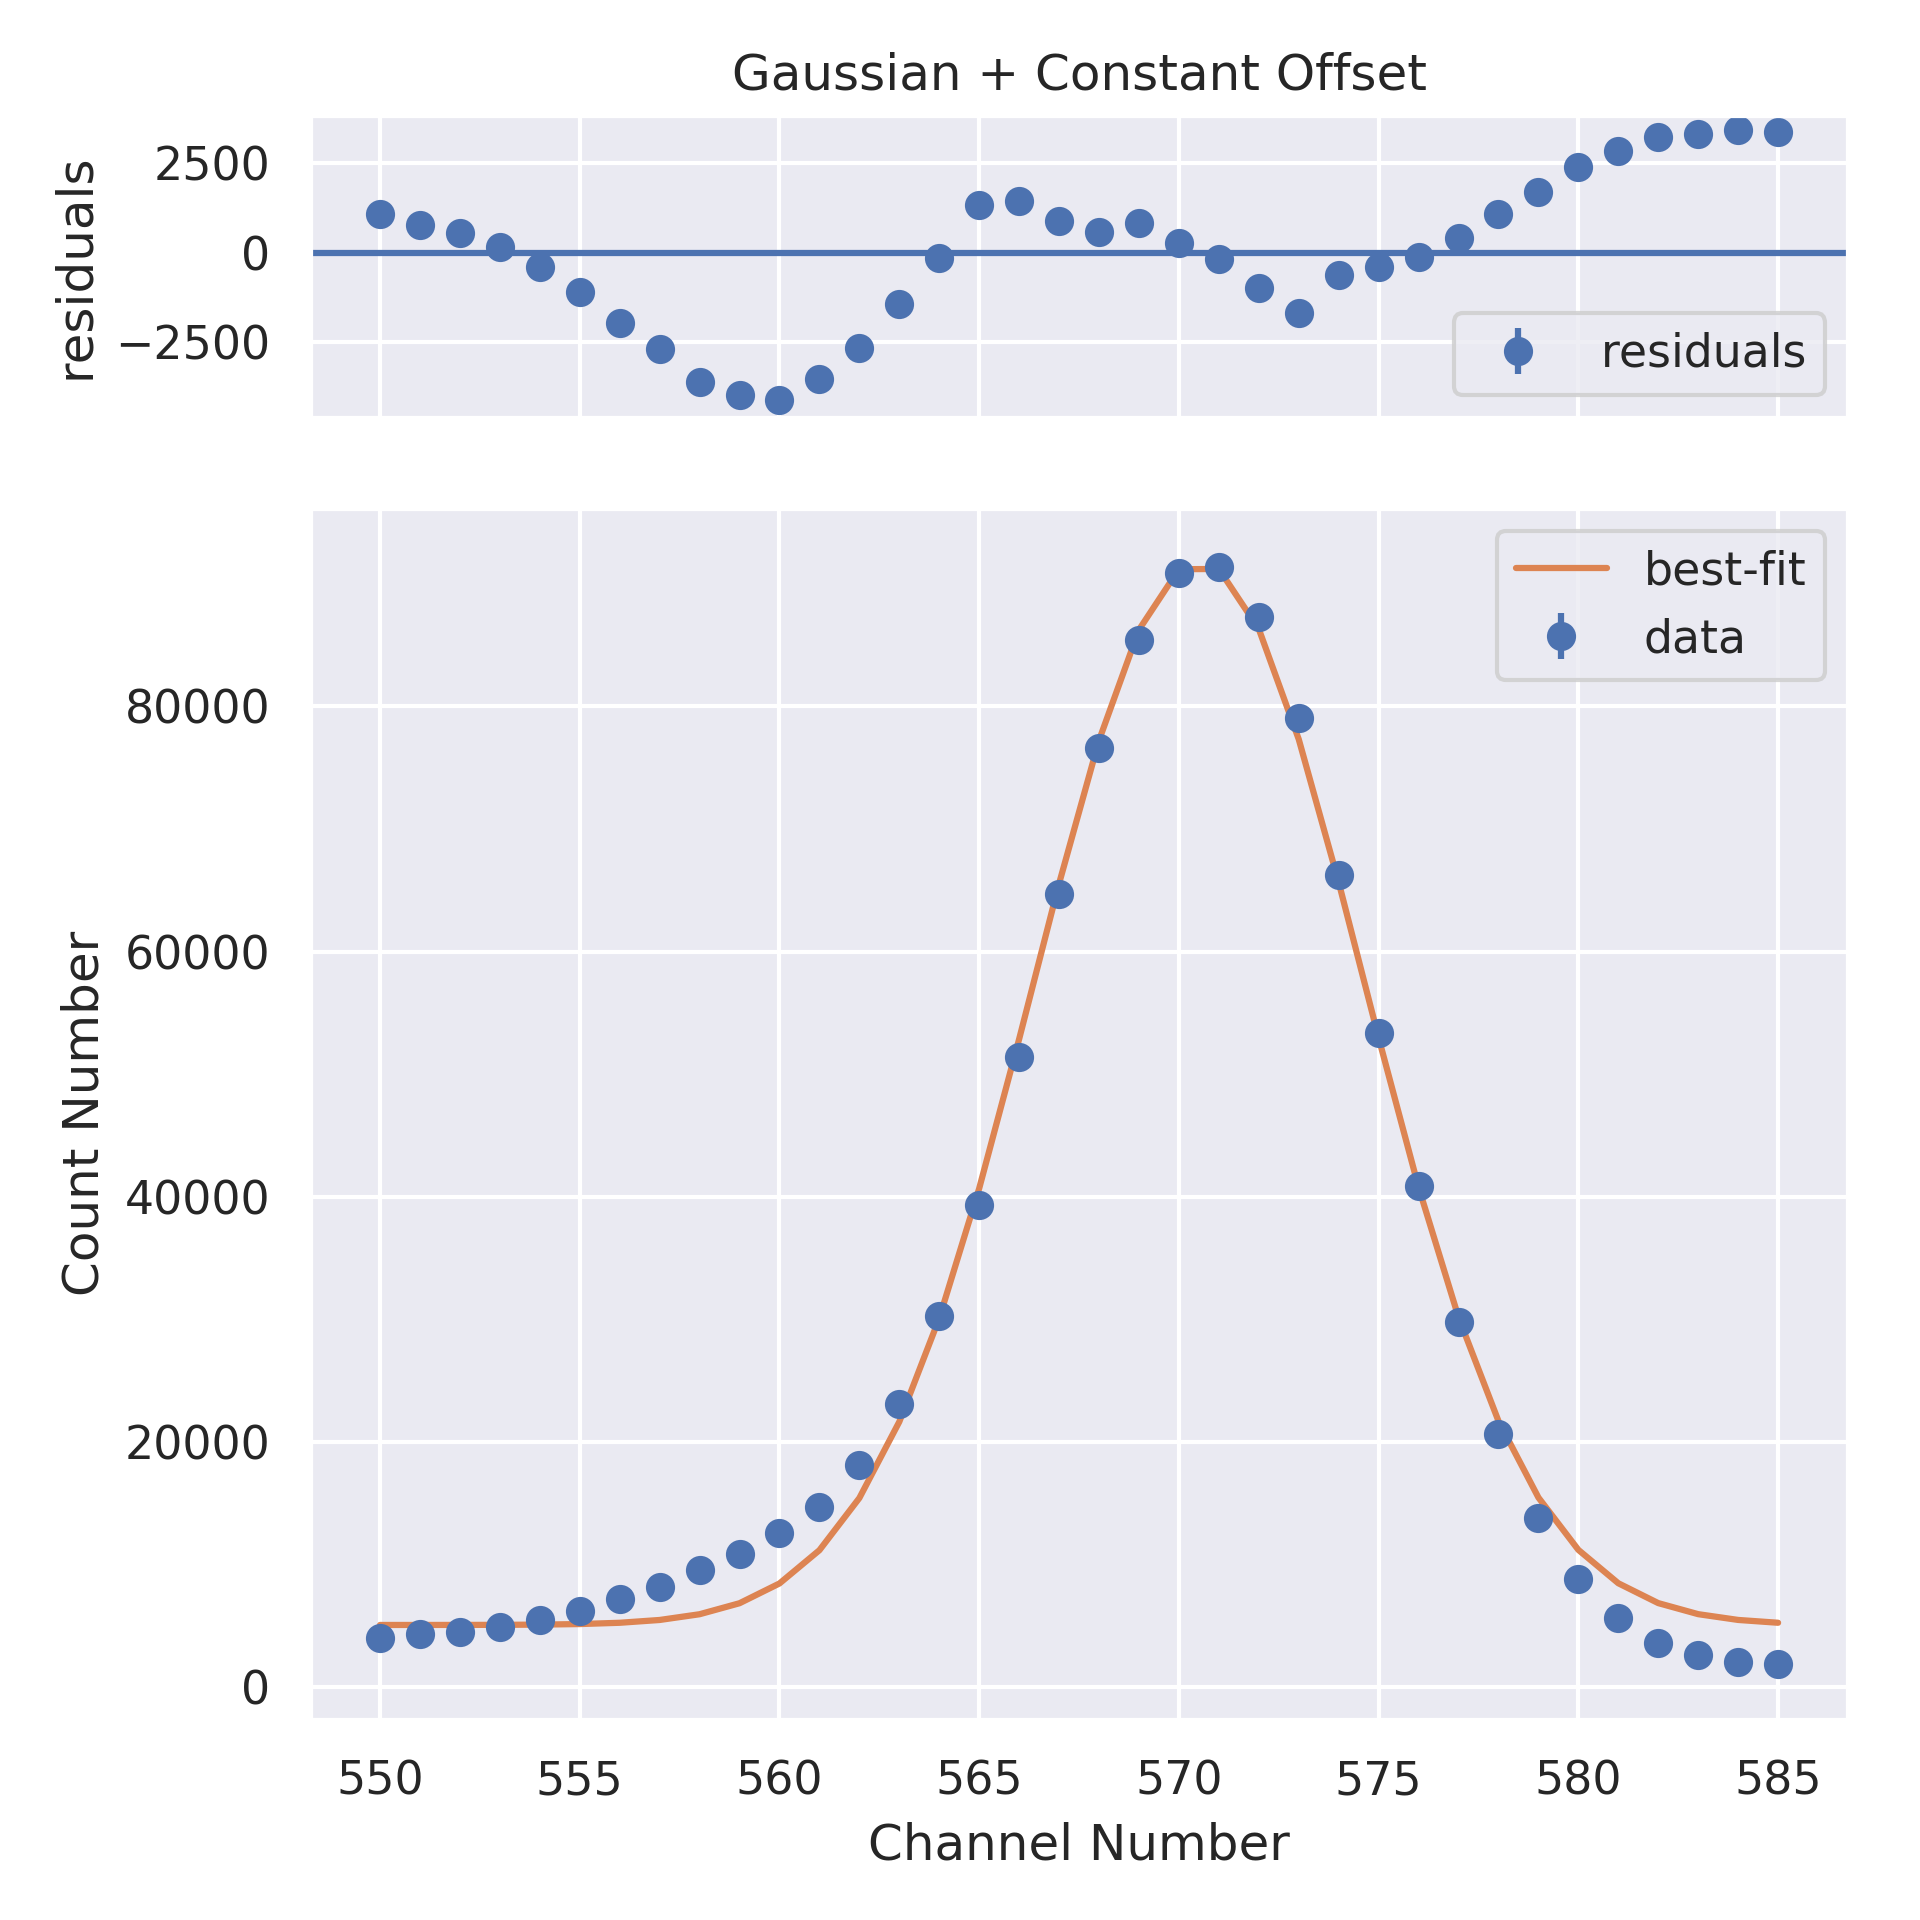
\includegraphics[width=\linewidth]{./Images/Barium133/Gauss/Gauss_1_Full.png}
    \caption{Full peak with fit. $\chi^2 = 29044$, $\chi^2_\nu = 854$, \\ Prob = 0\%, $\mu = 570.5$, $\sigma = 4.12$ }
    %\label{fig:sub1}
  \end{subfigure}%
  \begin{subfigure}{.5\linewidth}
    \centering
    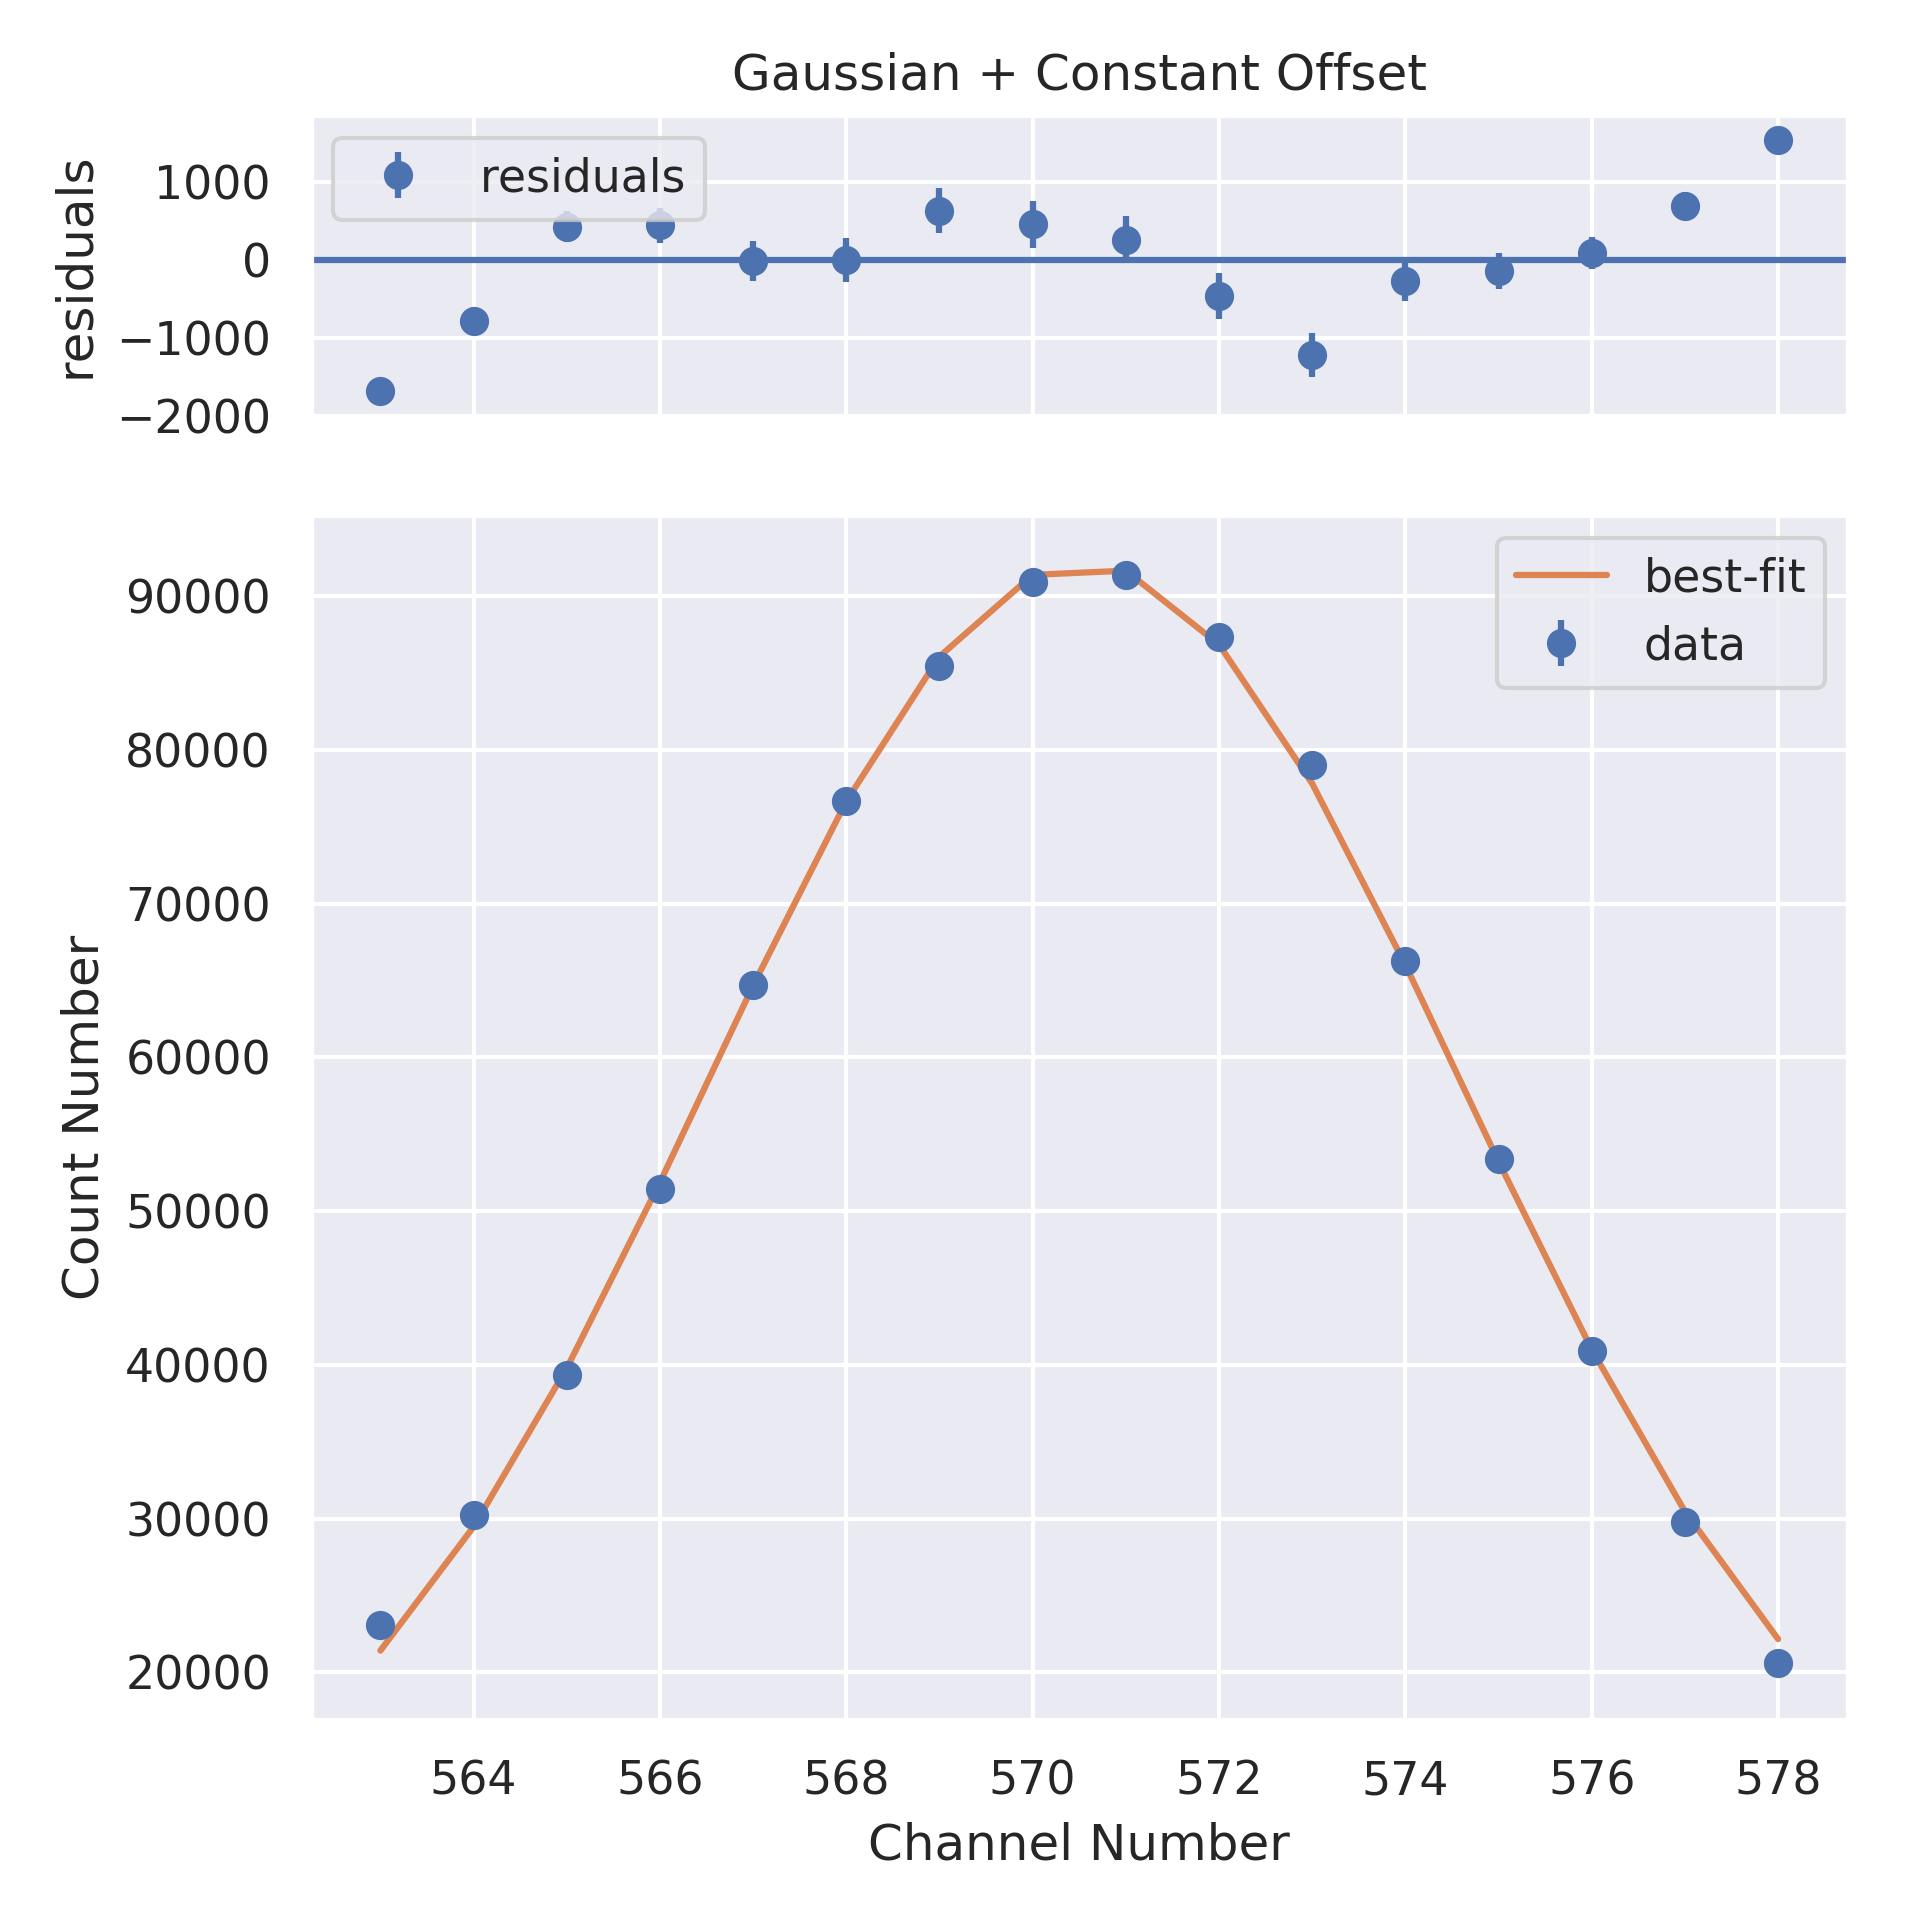
\includegraphics[width=\linewidth]{./Images/Barium133/Gauss/Gauss_1_Zoom.png}
    \caption{Zoomed in peak with fit. $\chi^2 = 310.6$, $\chi^2_\nu = 22.2$, \\ Prob = 0\%, $\mu = 570.6$, $\sigma = 4.00$}
    %\label{fig:sub2}
  \end{subfigure}
  \caption{Fit of full \& zoomed in peak of \element{Ba}{133} 81 keV peak}
  %\label{fig:test}
\end{figure}
\begin{figure}[H]
  \centering
  \begin{subfigure}{.5\linewidth}
    \centering
    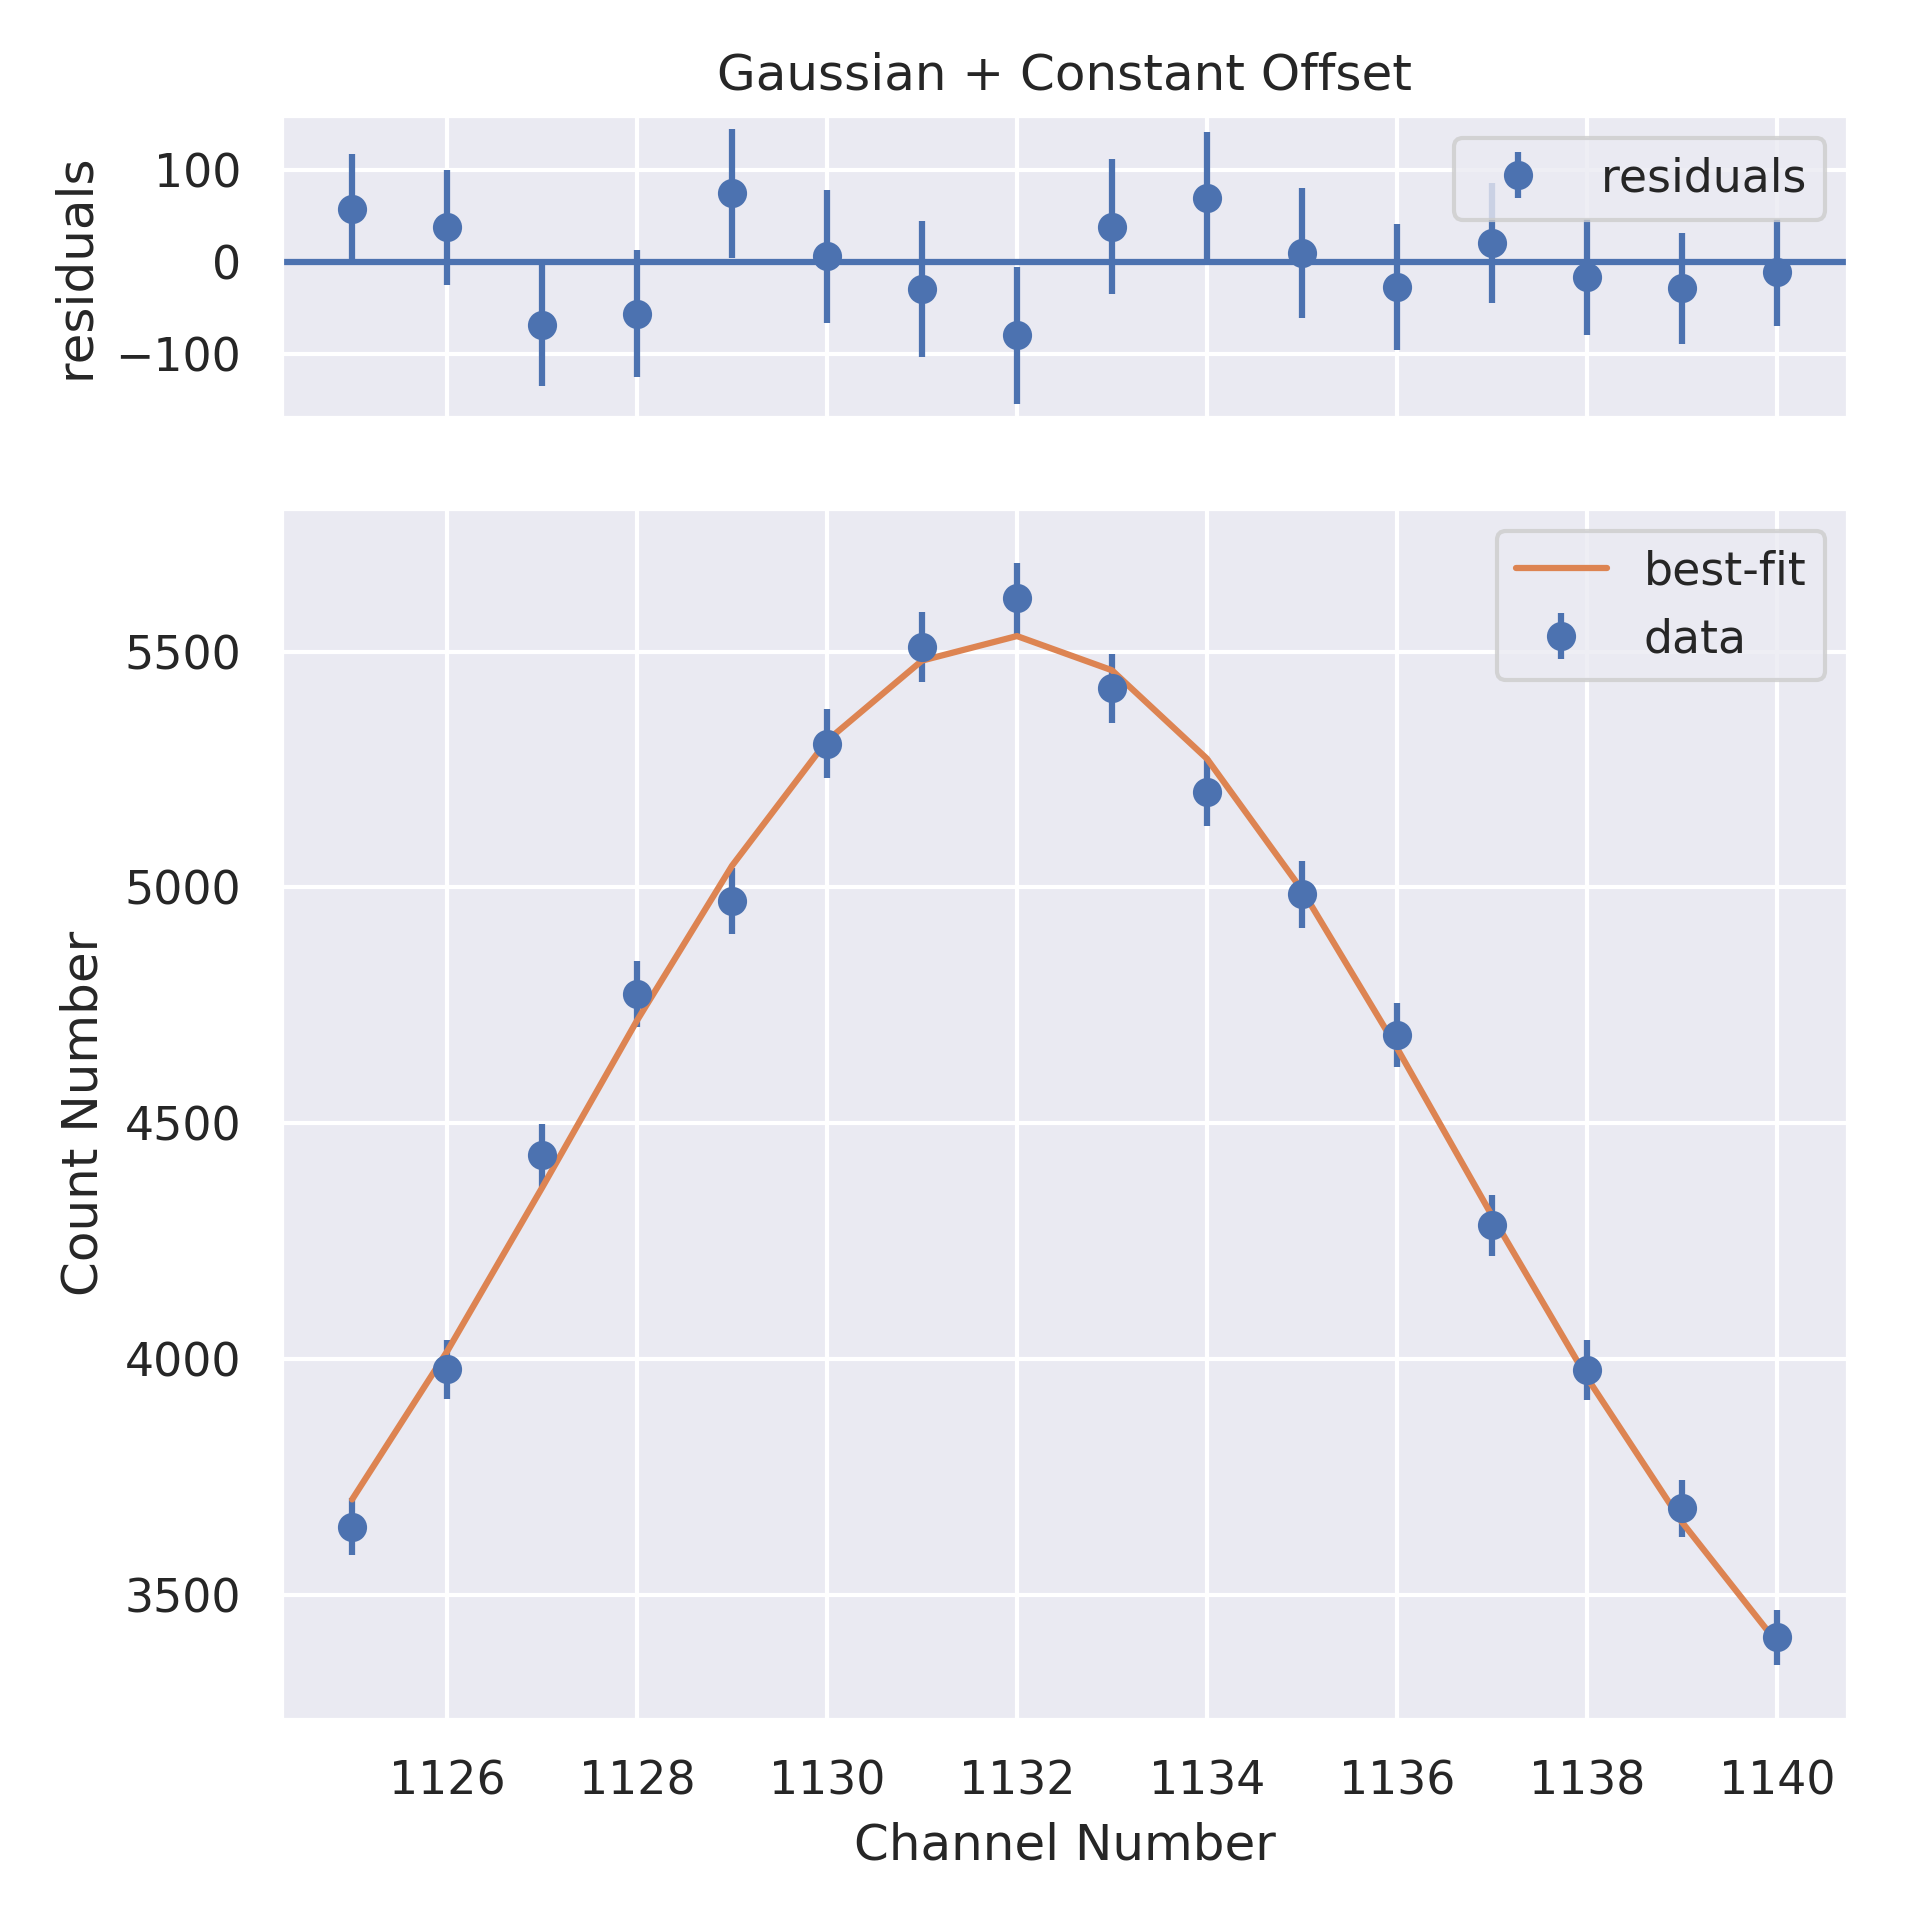
\includegraphics[width=\linewidth]{./Images/Barium133/Gauss/Gauss_2_Full.png}
    \caption{Full peak with fit. $\chi^2 = 7.26$, $\chi^2_\nu = 0.52$, \\ Prob = 92.4\%, $\mu = 1131.9$, $\sigma = 4.7$}
    %\label{fig:sub1}
  \end{subfigure}%
  \begin{subfigure}{.5\linewidth}
    \centering
    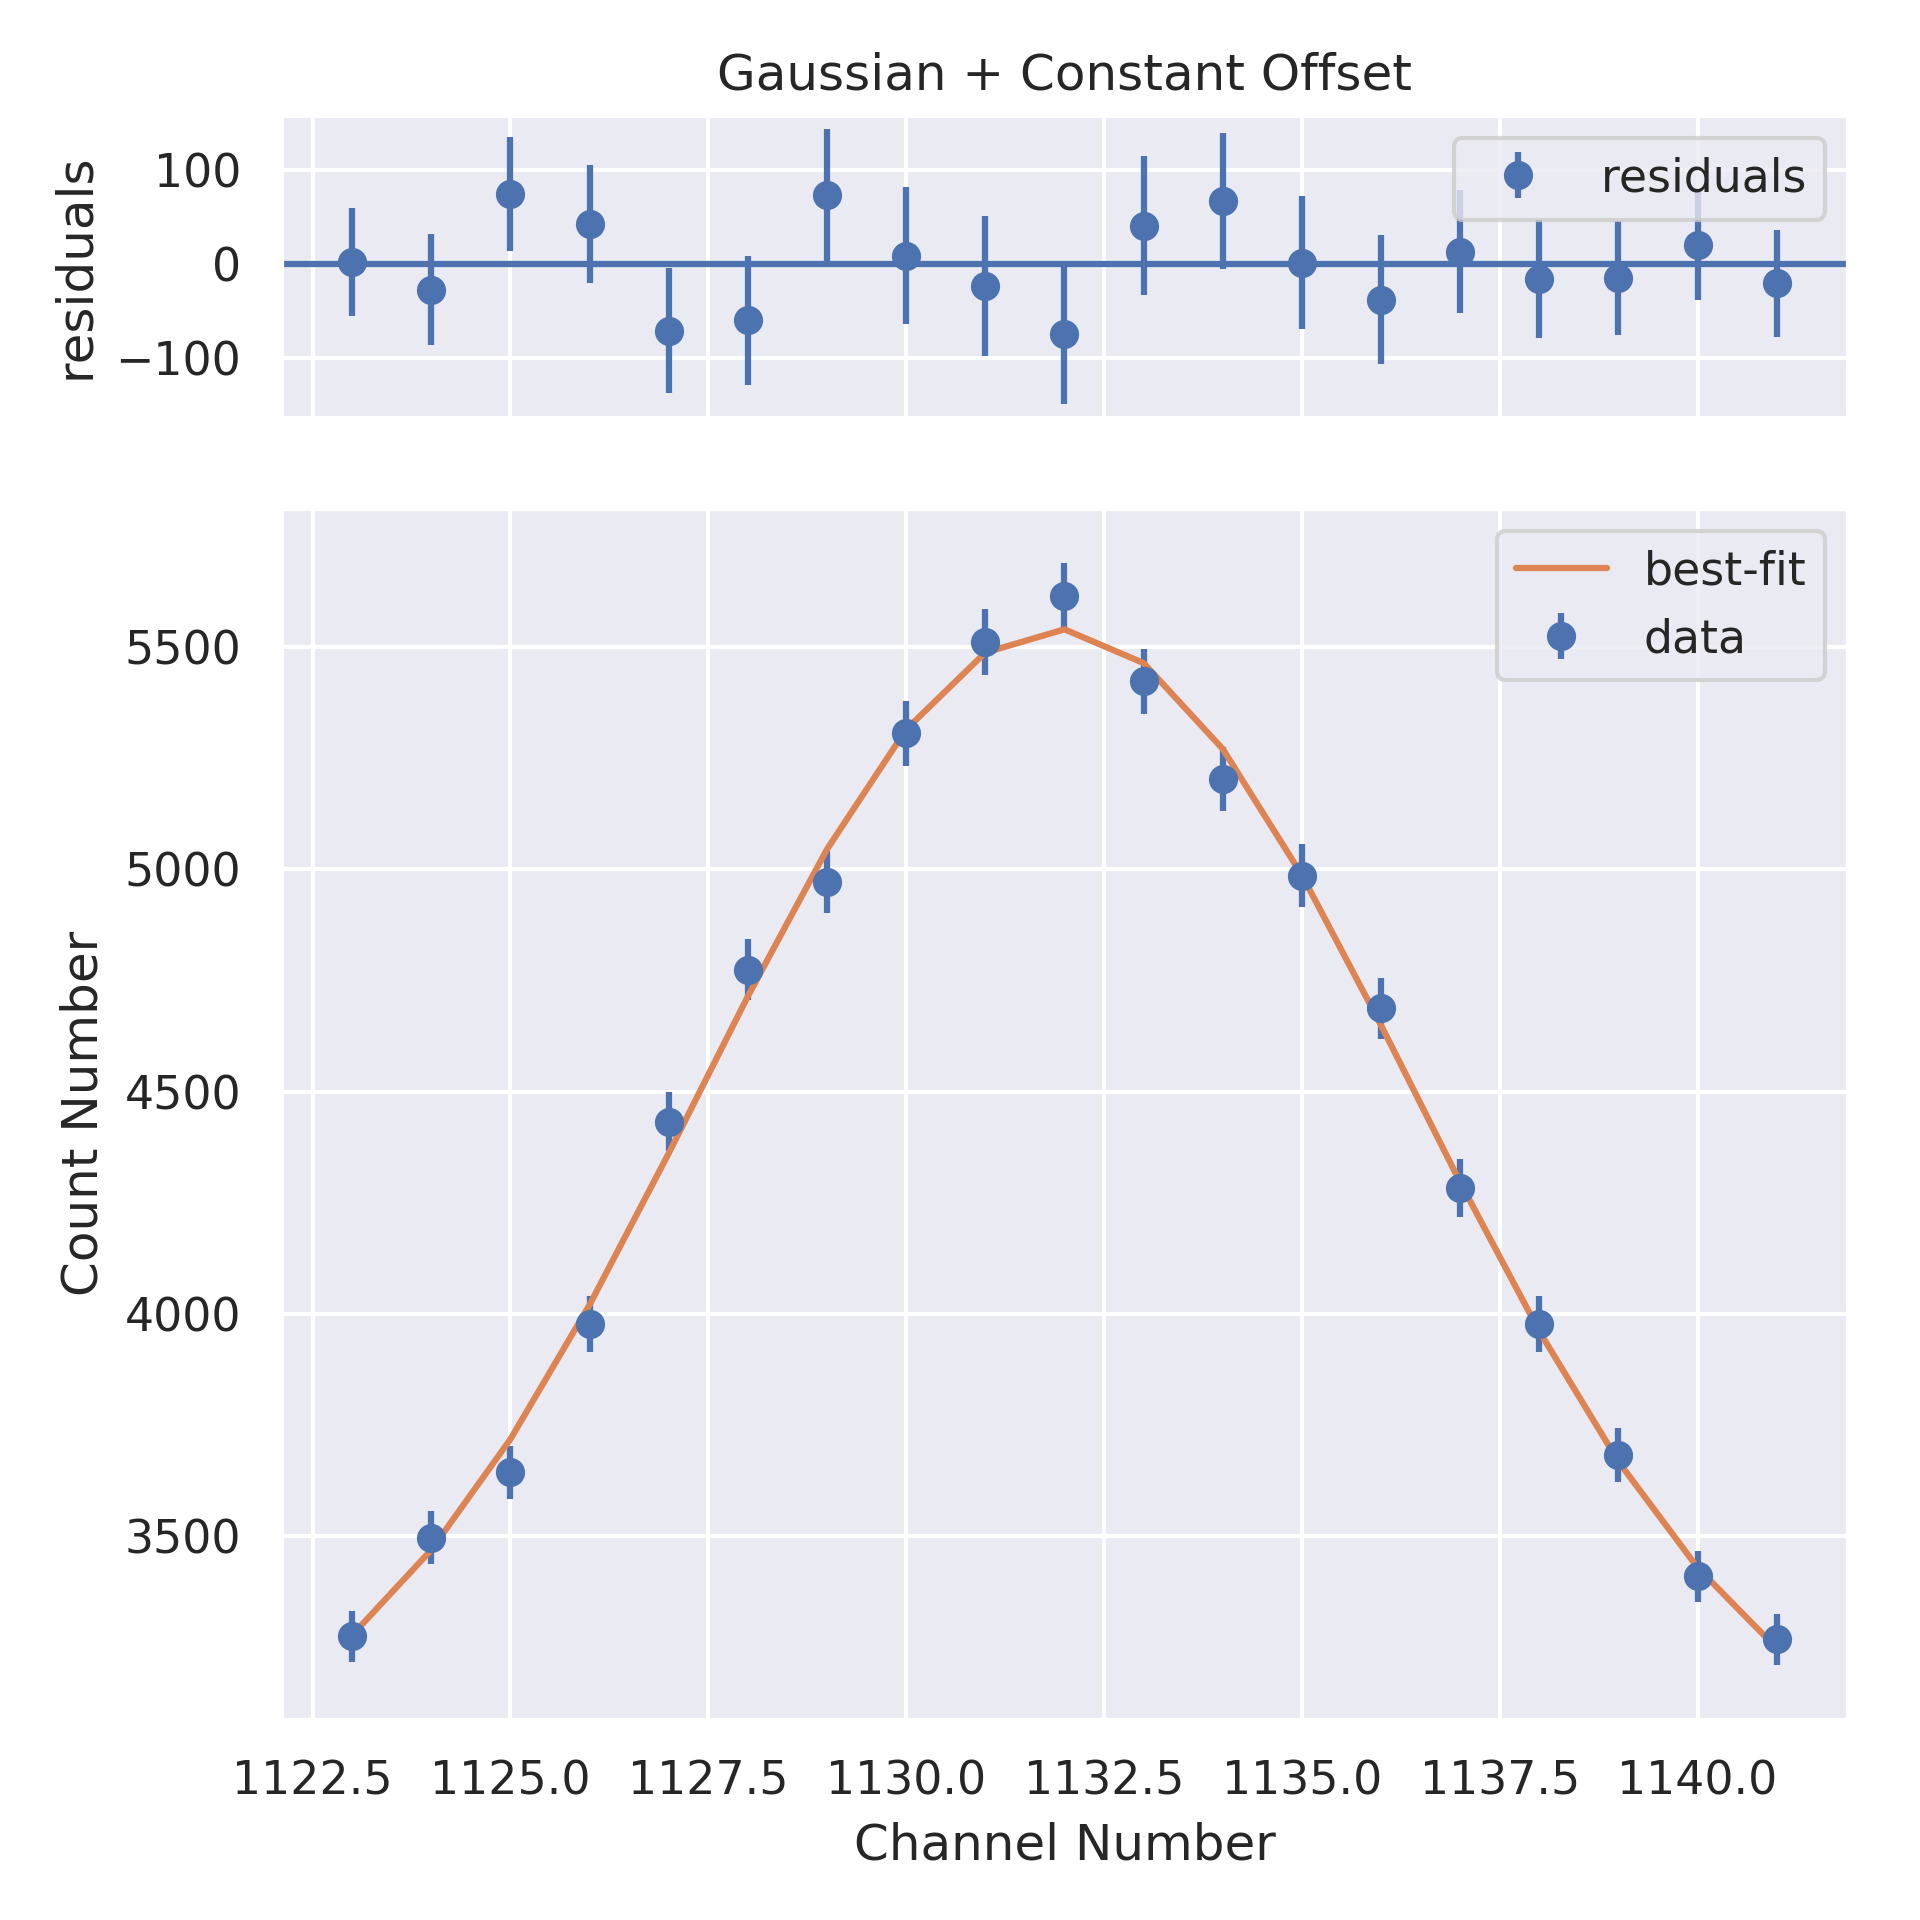
\includegraphics[width=\linewidth]{./Images/Barium133/Gauss/Gauss_2_Zoom.png}
    \caption{Zoomed in peak with fit. $\chi^2 = 8.16$, $\chi^2_\nu = 0.48$, \\ Prob = 96.3\%, $\mu = 1131.9$, $\sigma = 4.51$}
    %\label{fig:sub2}
  \end{subfigure}
  \caption{Fit of full \& zoomed in peak of \element{Ba}{133} 161 keV peak}
  %\label{fig:test}
\end{figure}
\begin{figure}[H]
  \centering
  \begin{subfigure}{.5\linewidth}
    \centering
    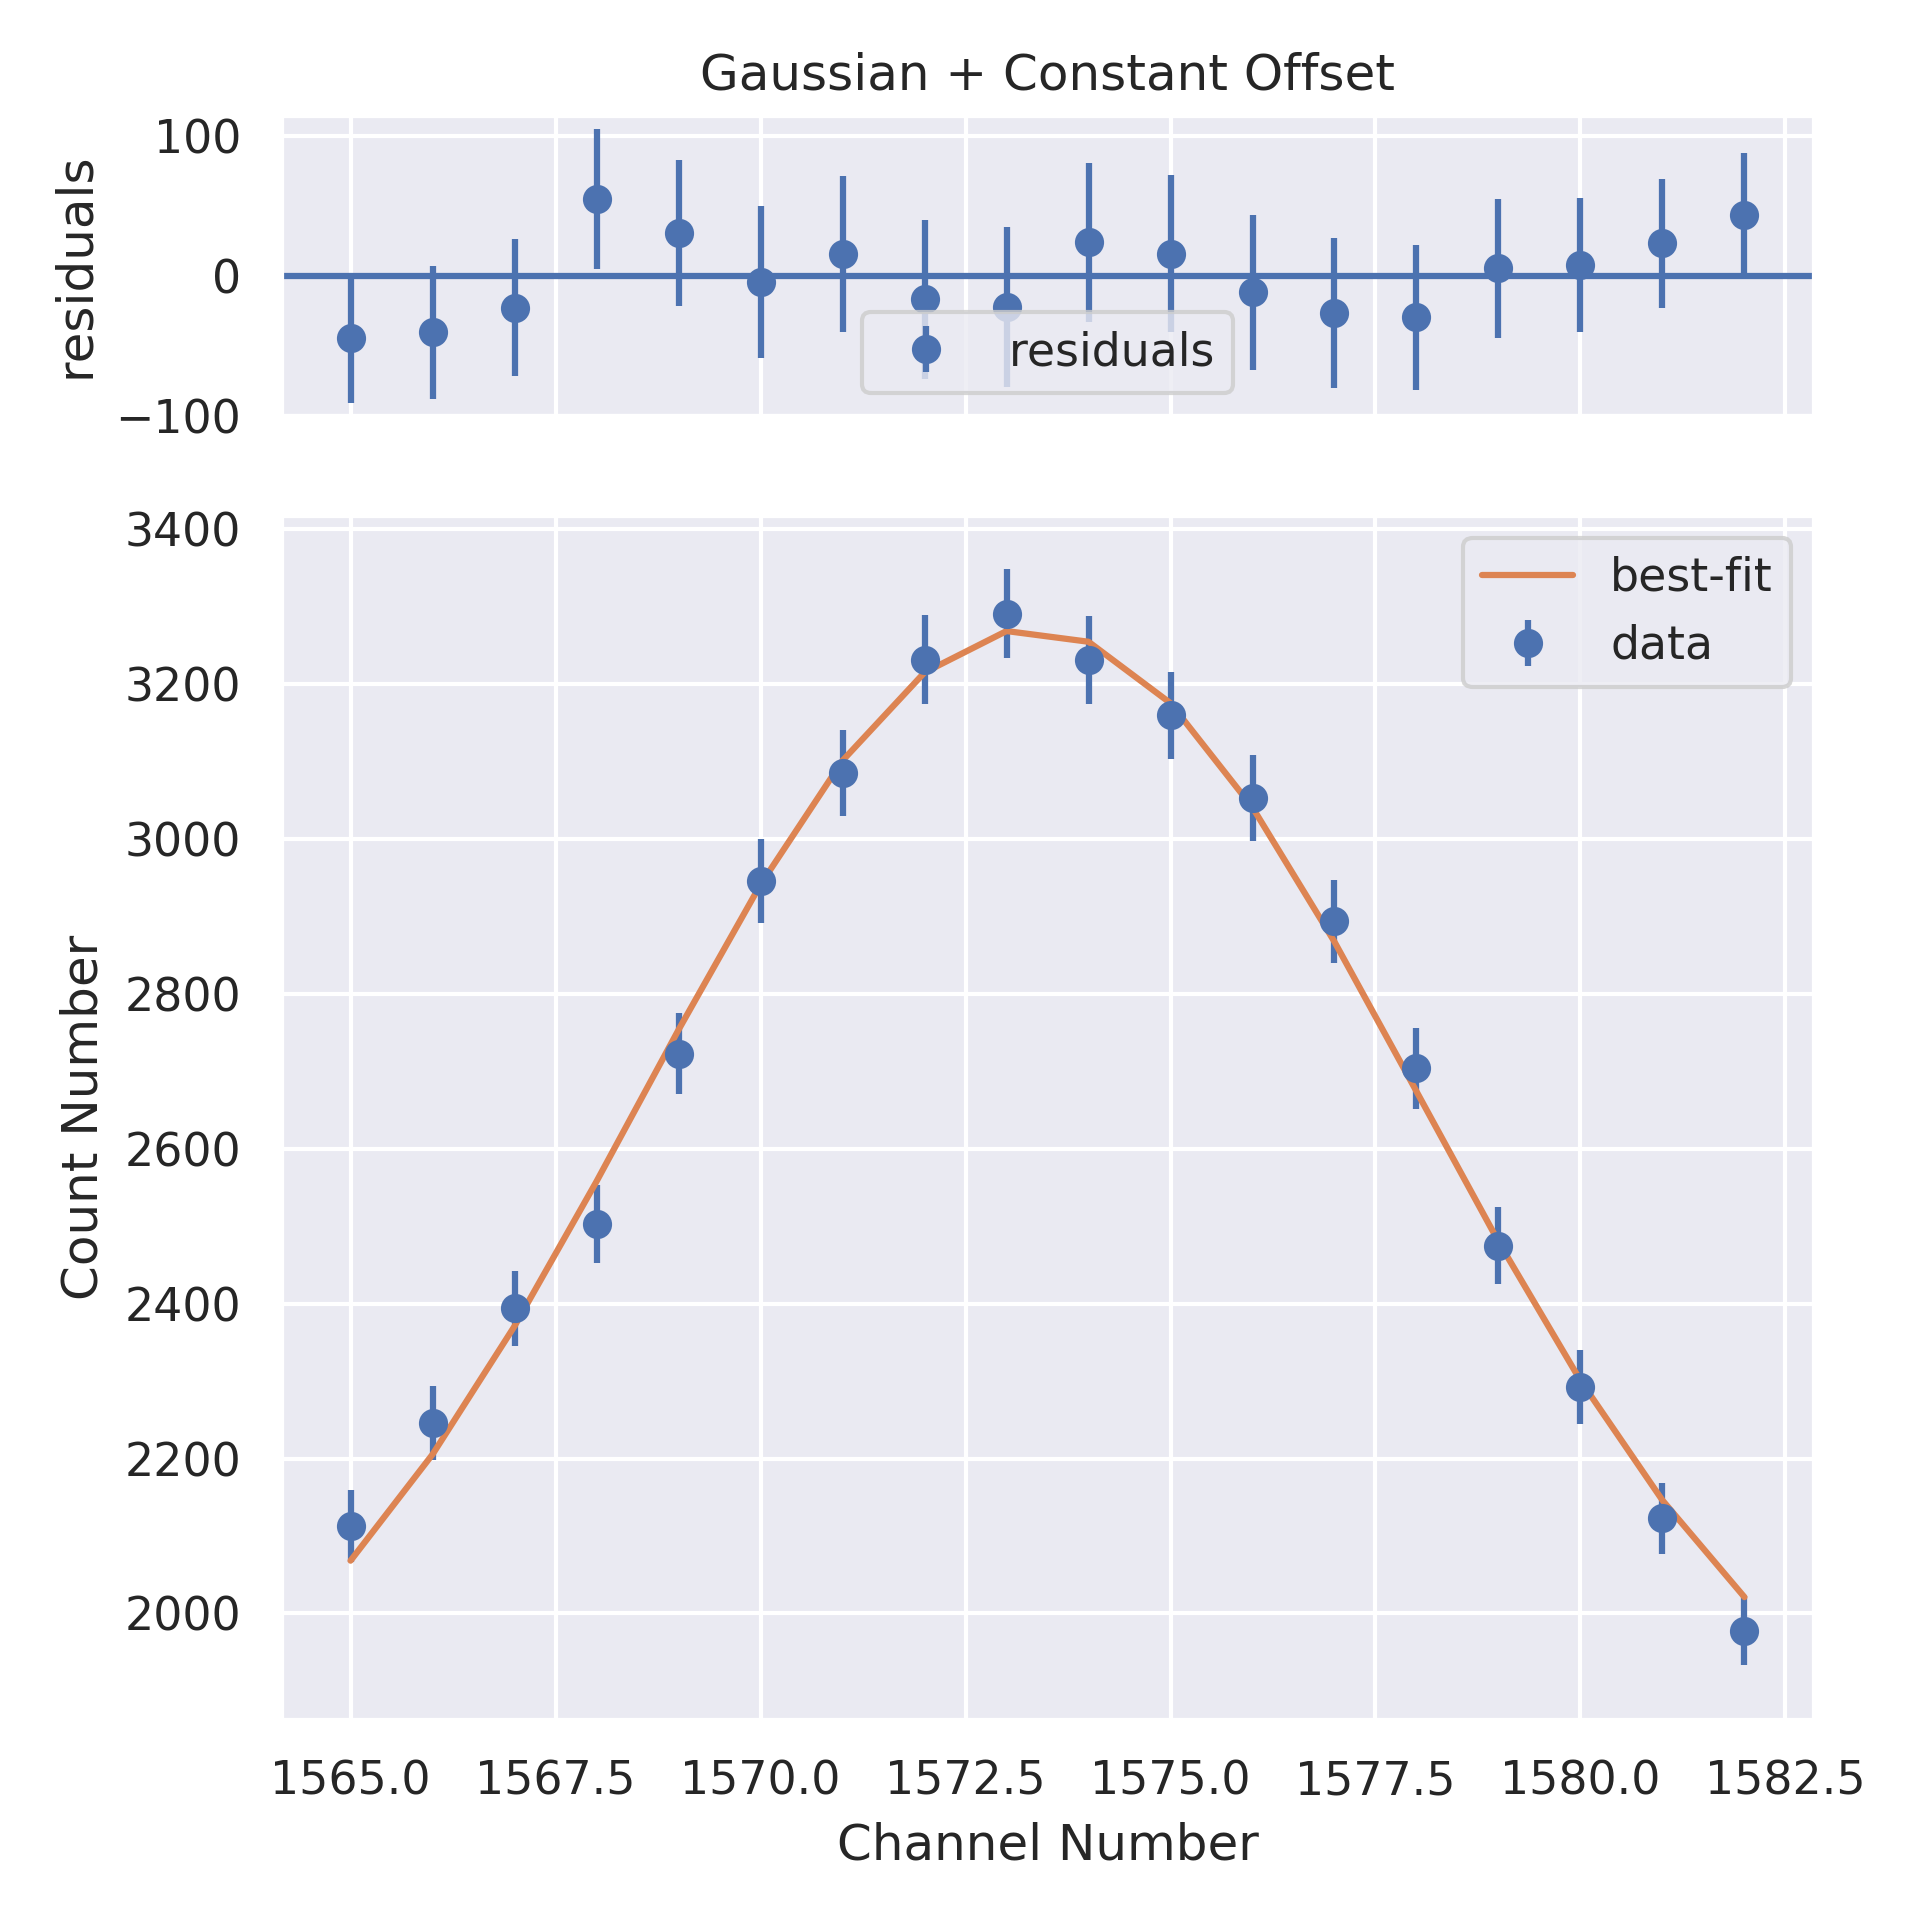
\includegraphics[width=\linewidth]{./Images/Barium133/Gauss/Gauss_3_Full.png}
    \caption{Full peak with fit. $\chi^2 = 5.88$, $\chi^2_\nu = 0.36$, \\ Prob = 98.93\%, $\mu = 1573.29$, $\sigma = 4.73$}
    %\label{fig:sub1}
  \end{subfigure}%
  \begin{subfigure}{.5\linewidth}
    \centering
    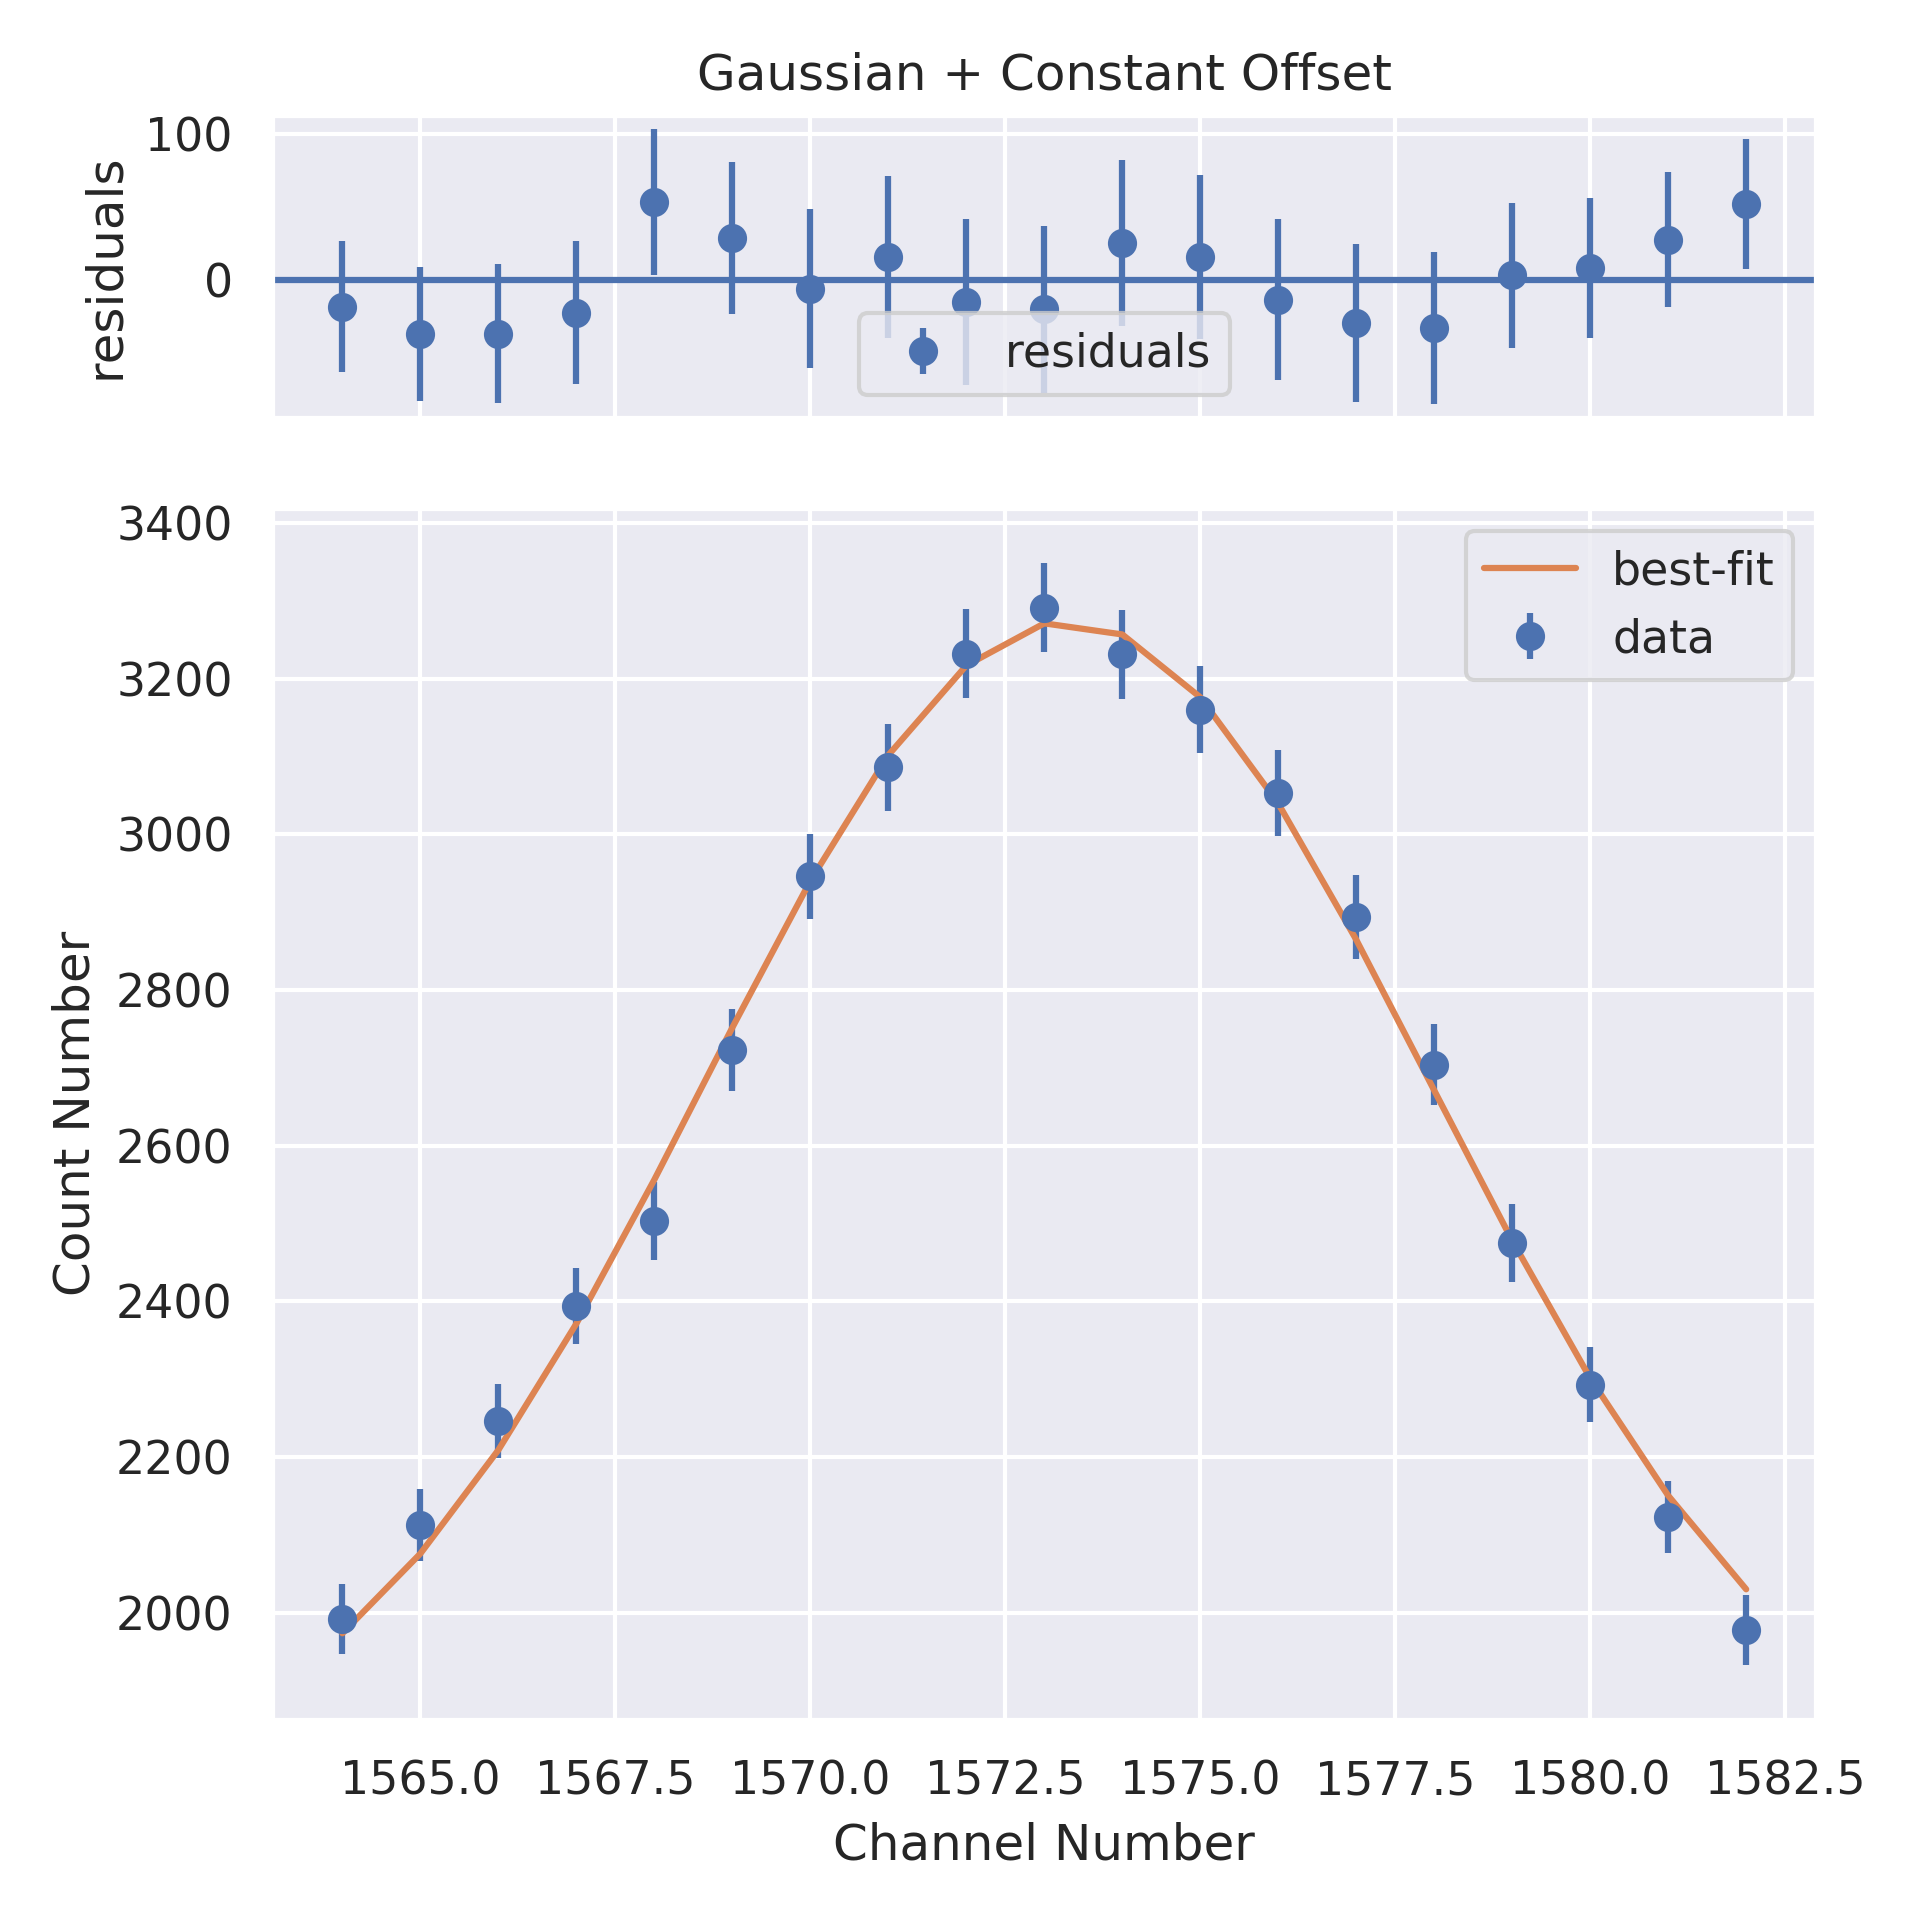
\includegraphics[width=\linewidth]{./Images/Barium133/Gauss/Gauss_3_Zoom.png}
    \caption{Zoomed in peak with fit. $\chi^2 = 6.18$, $\chi^2_\nu = 0.36$, \\ Prob = 99.19\%, $\mu = 1573.23$, $\sigma = 4.65$}
    %\label{fig:sub2}
  \end{subfigure}
  \caption{Fit of full \& zoomed in peak of \element{Ba}{133} 223 keV peak}
  %\label{fig:test}
\end{figure}
\begin{figure}[H]
  \centering
  \begin{subfigure}{.5\linewidth}
    \centering
    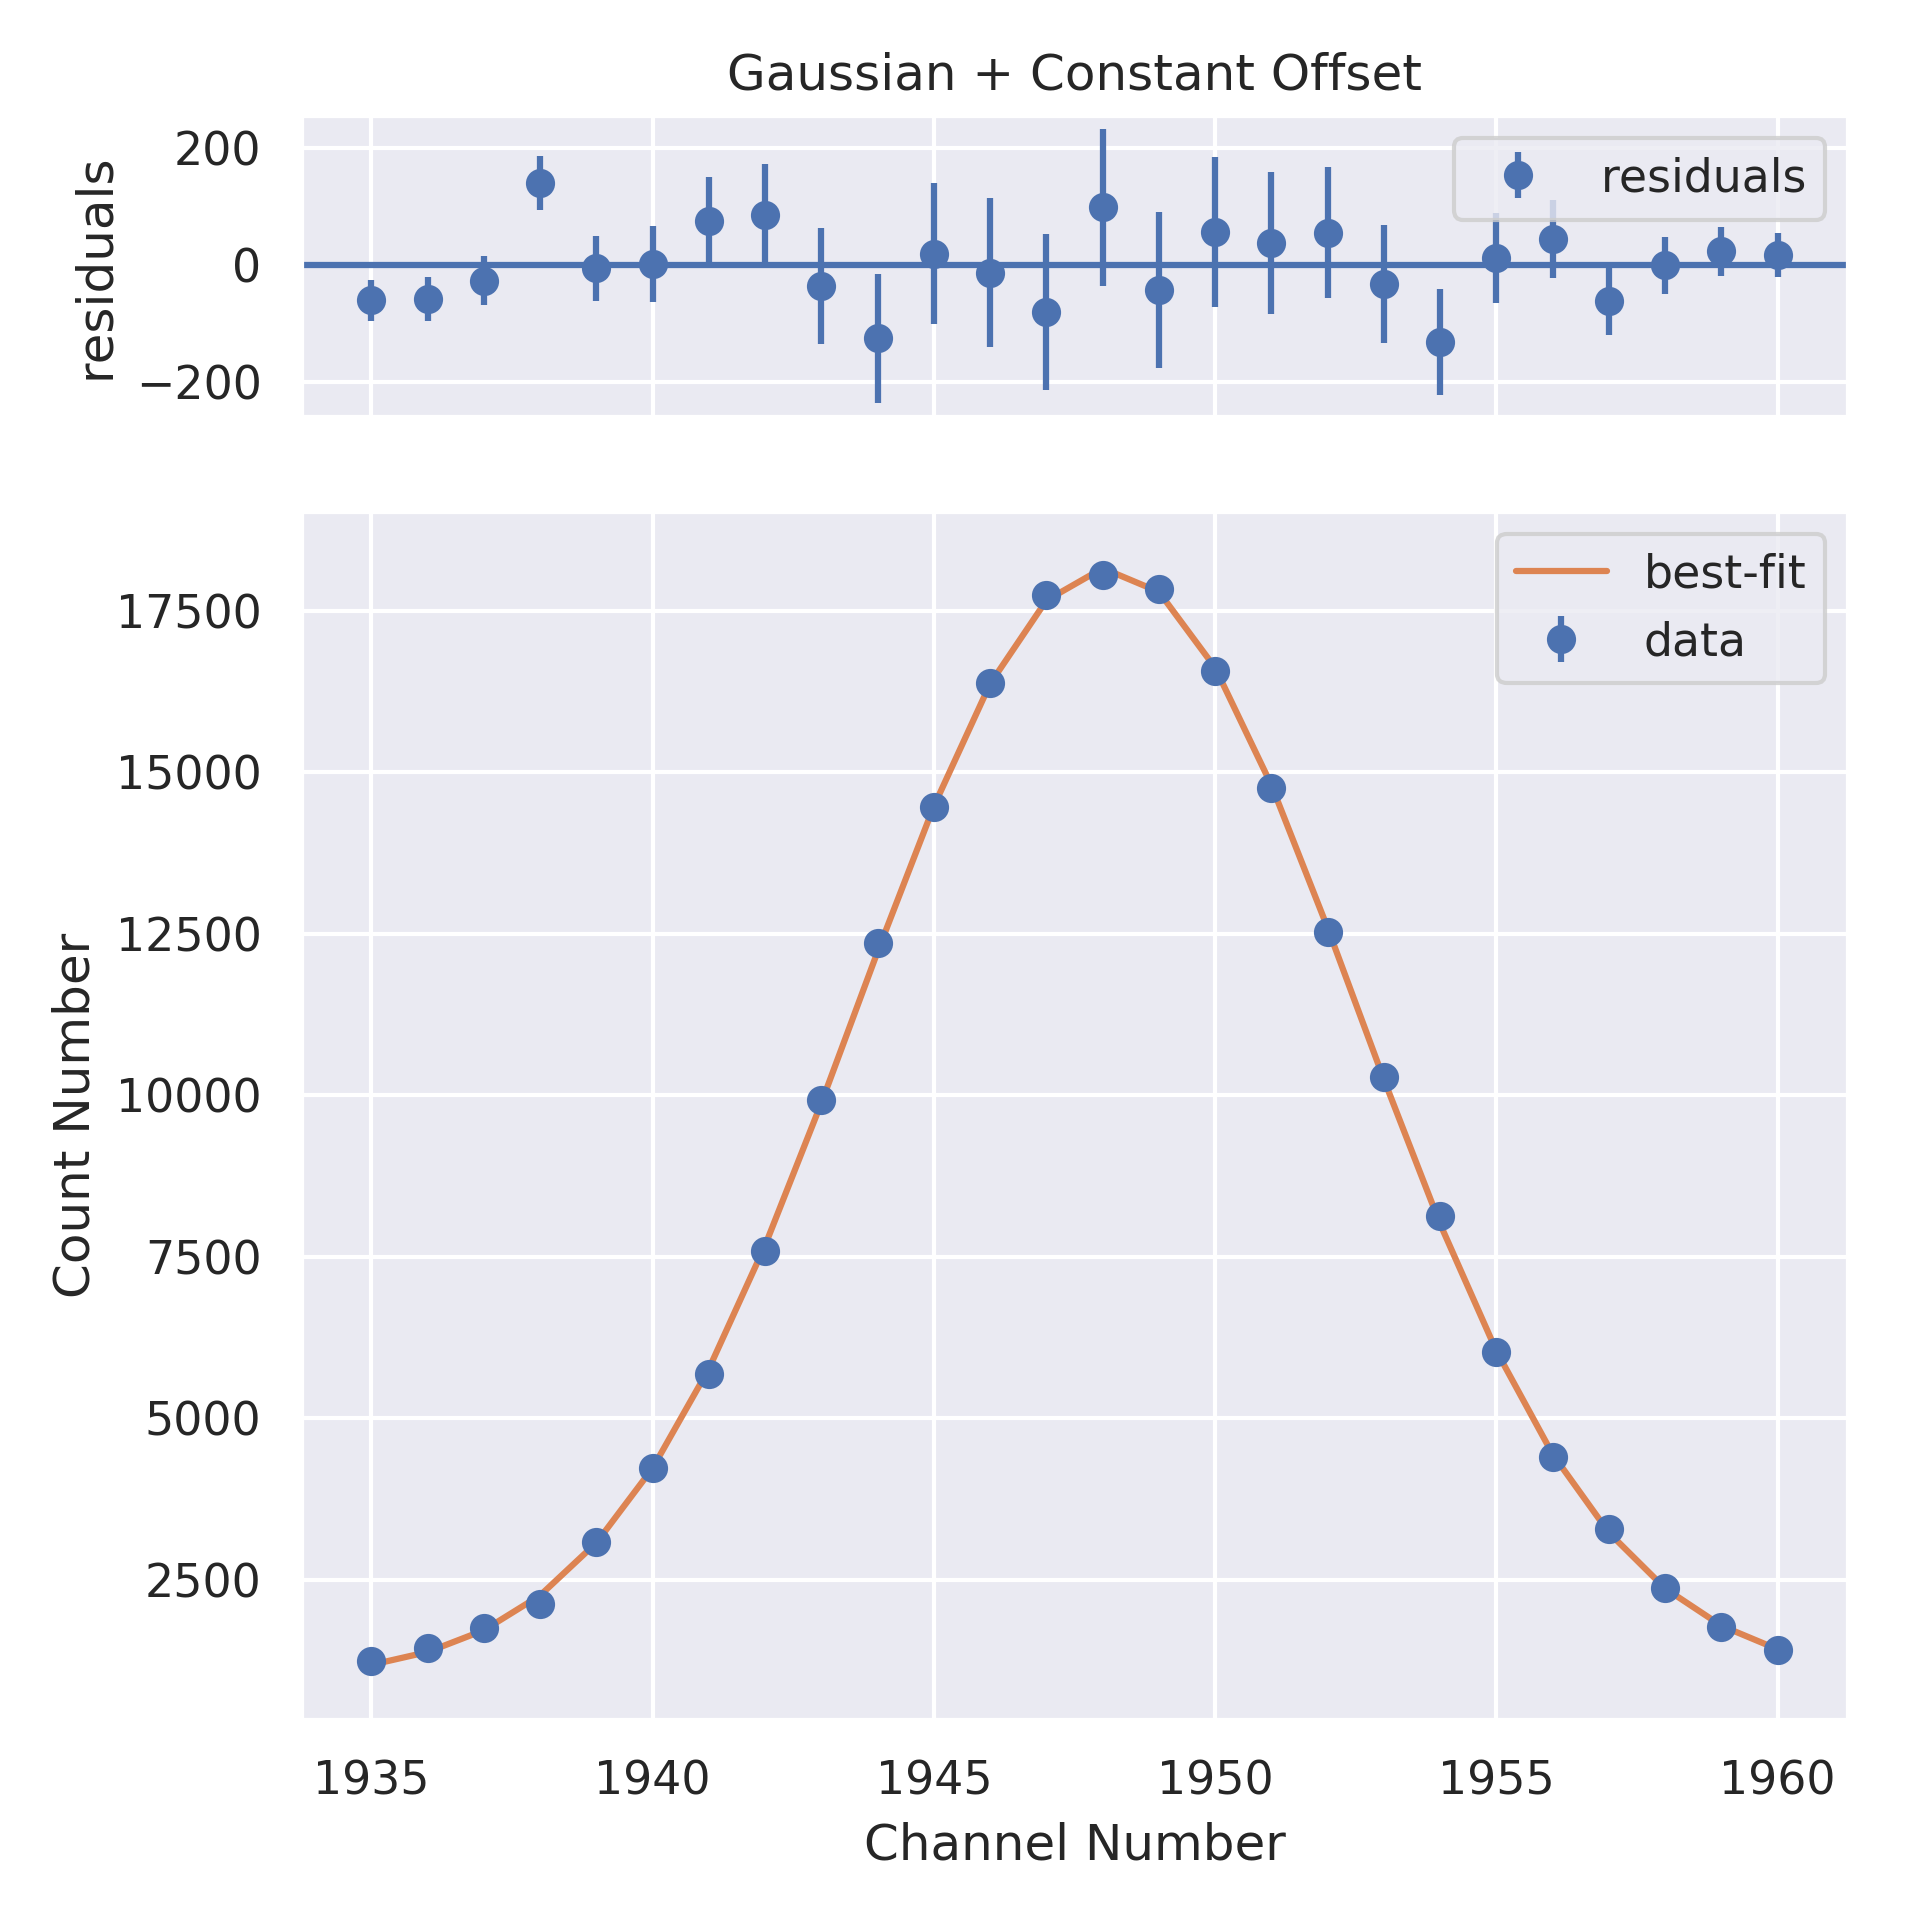
\includegraphics[width=\linewidth]{./Images/Barium133/Gauss/Gauss_4_Full.png}
    \caption{Full peak with fit. $\chi^2 = 24.2$, $\chi^2_\nu = 1.01$, \\ Prob = 44.9\%, $\mu = 1948.1$, $\sigma = 4.43$}
    %\label{fig:sub1}
  \end{subfigure}%
  \begin{subfigure}{.5\linewidth}
    \centering
    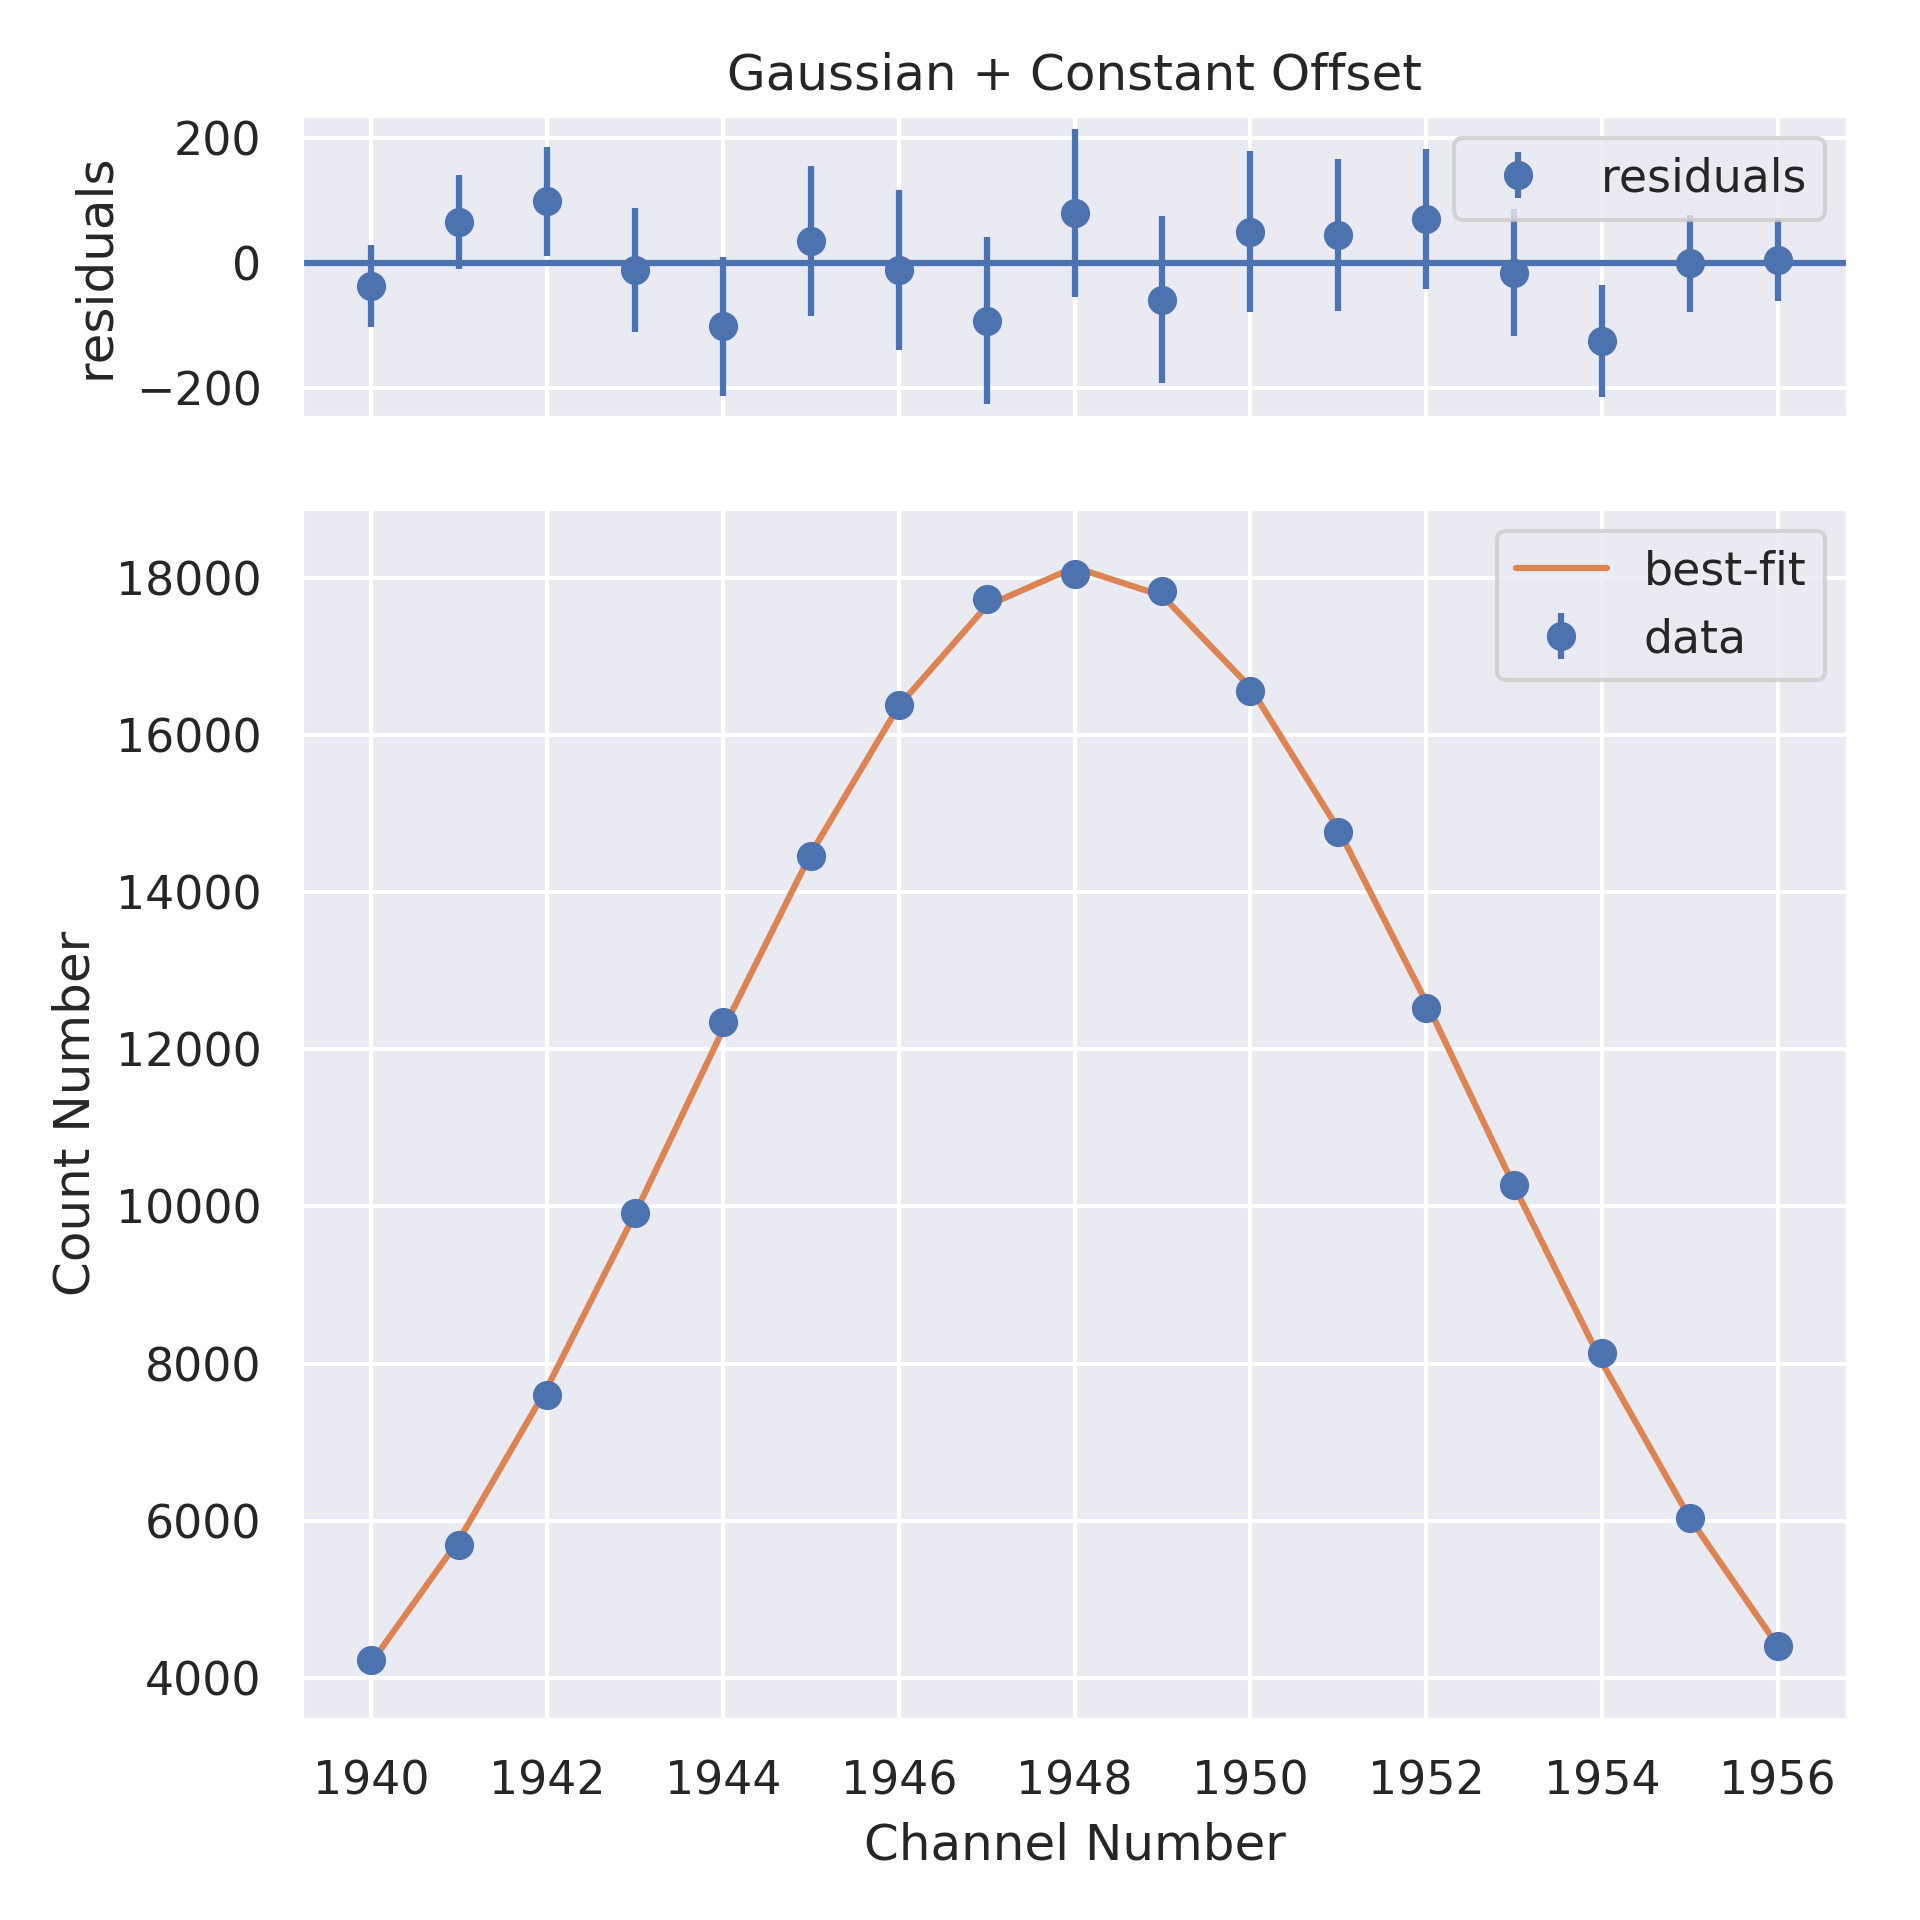
\includegraphics[width=\linewidth]{./Images/Barium133/Gauss/Gauss_4_Zoom.png}
    \caption{Zoomed in peak with fit. $\chi^2 = 6.92$, $\chi^2_\nu = 0.46$, \\ Prob = 96.0\%, $\mu = 1948.1$, $\sigma = 4.48$}
    %\label{fig:sub2}
  \end{subfigure}
  \caption{Fit of full \& zoomed in peak of \element{Ba}{133} 276 keV peak}
  %\label{fig:test}
\end{figure}
\begin{figure}[H]
  \centering
  \begin{subfigure}{.5\linewidth}
    \centering
    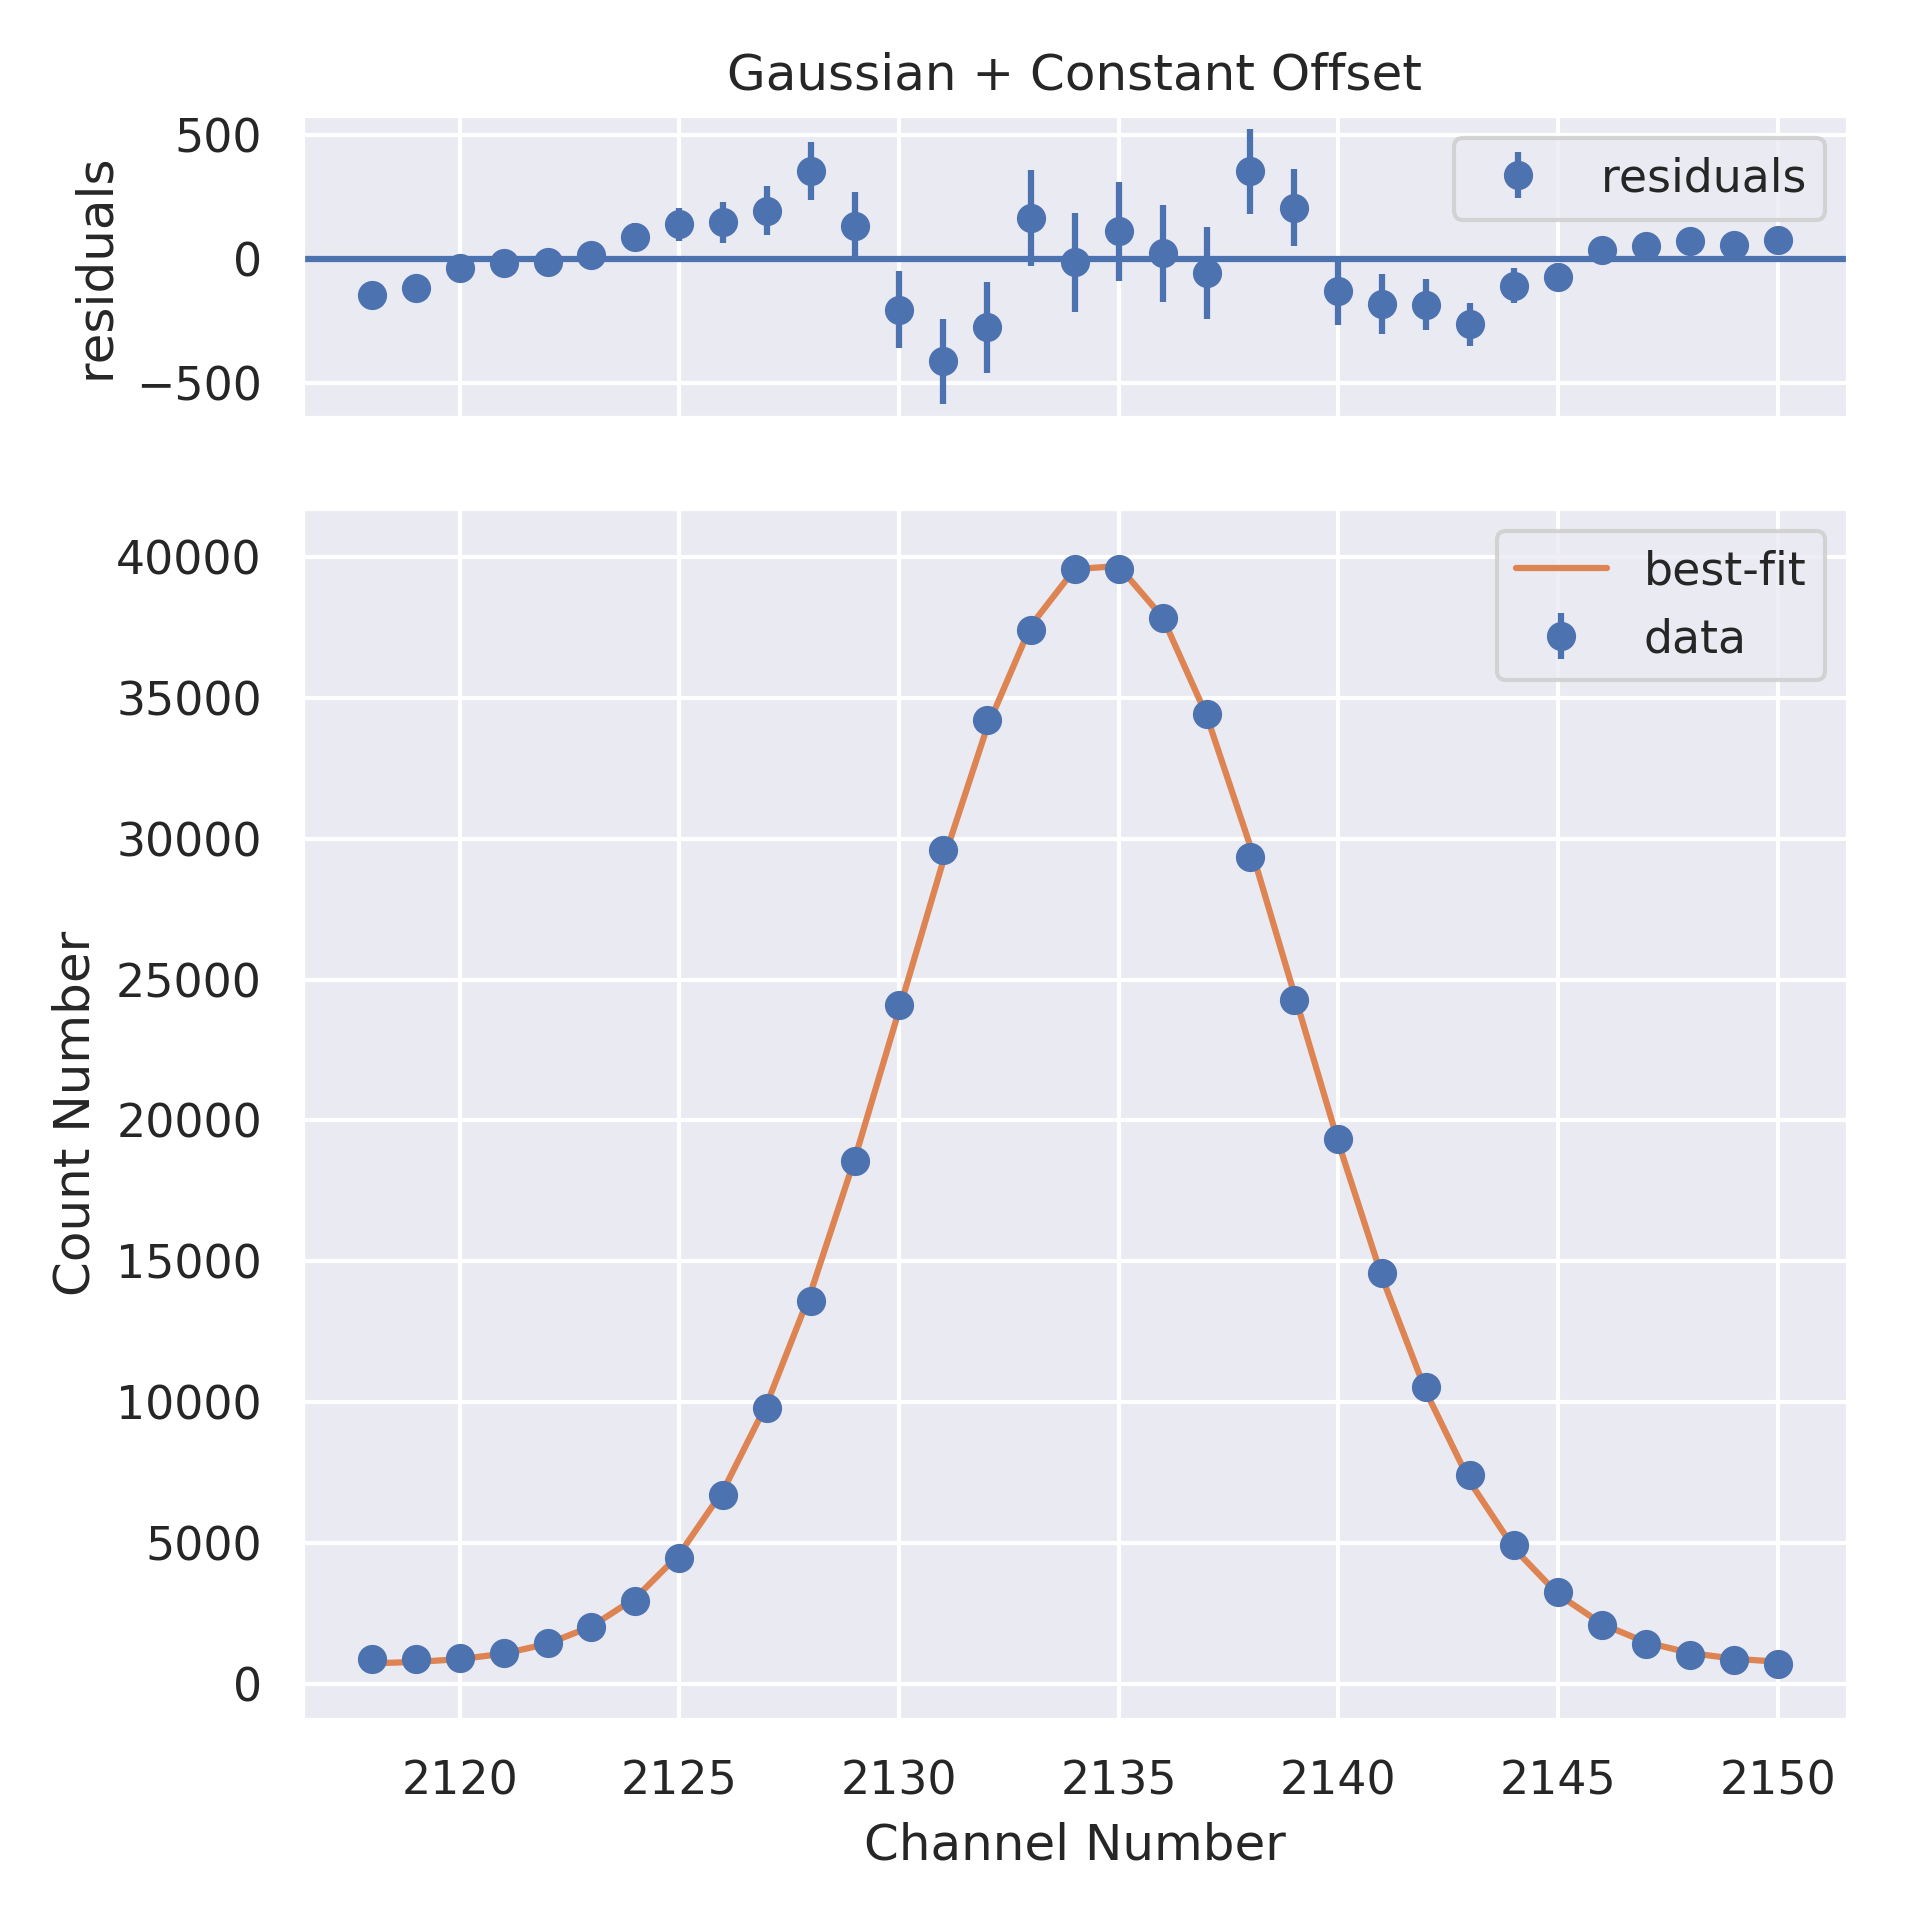
\includegraphics[width=\linewidth]{./Images/Barium133/Gauss/Gauss_5_Full.png}
    \caption{Full peak with fit. $\chi^2 = 121$, $\chi^2_\nu = 4$, \\ Prob = 0\%, $\mu = 2134.55$, $\sigma = 4.45$}
    %\label{fig:sub1}
  \end{subfigure}%
  \begin{subfigure}{.5\linewidth}
    \centering
    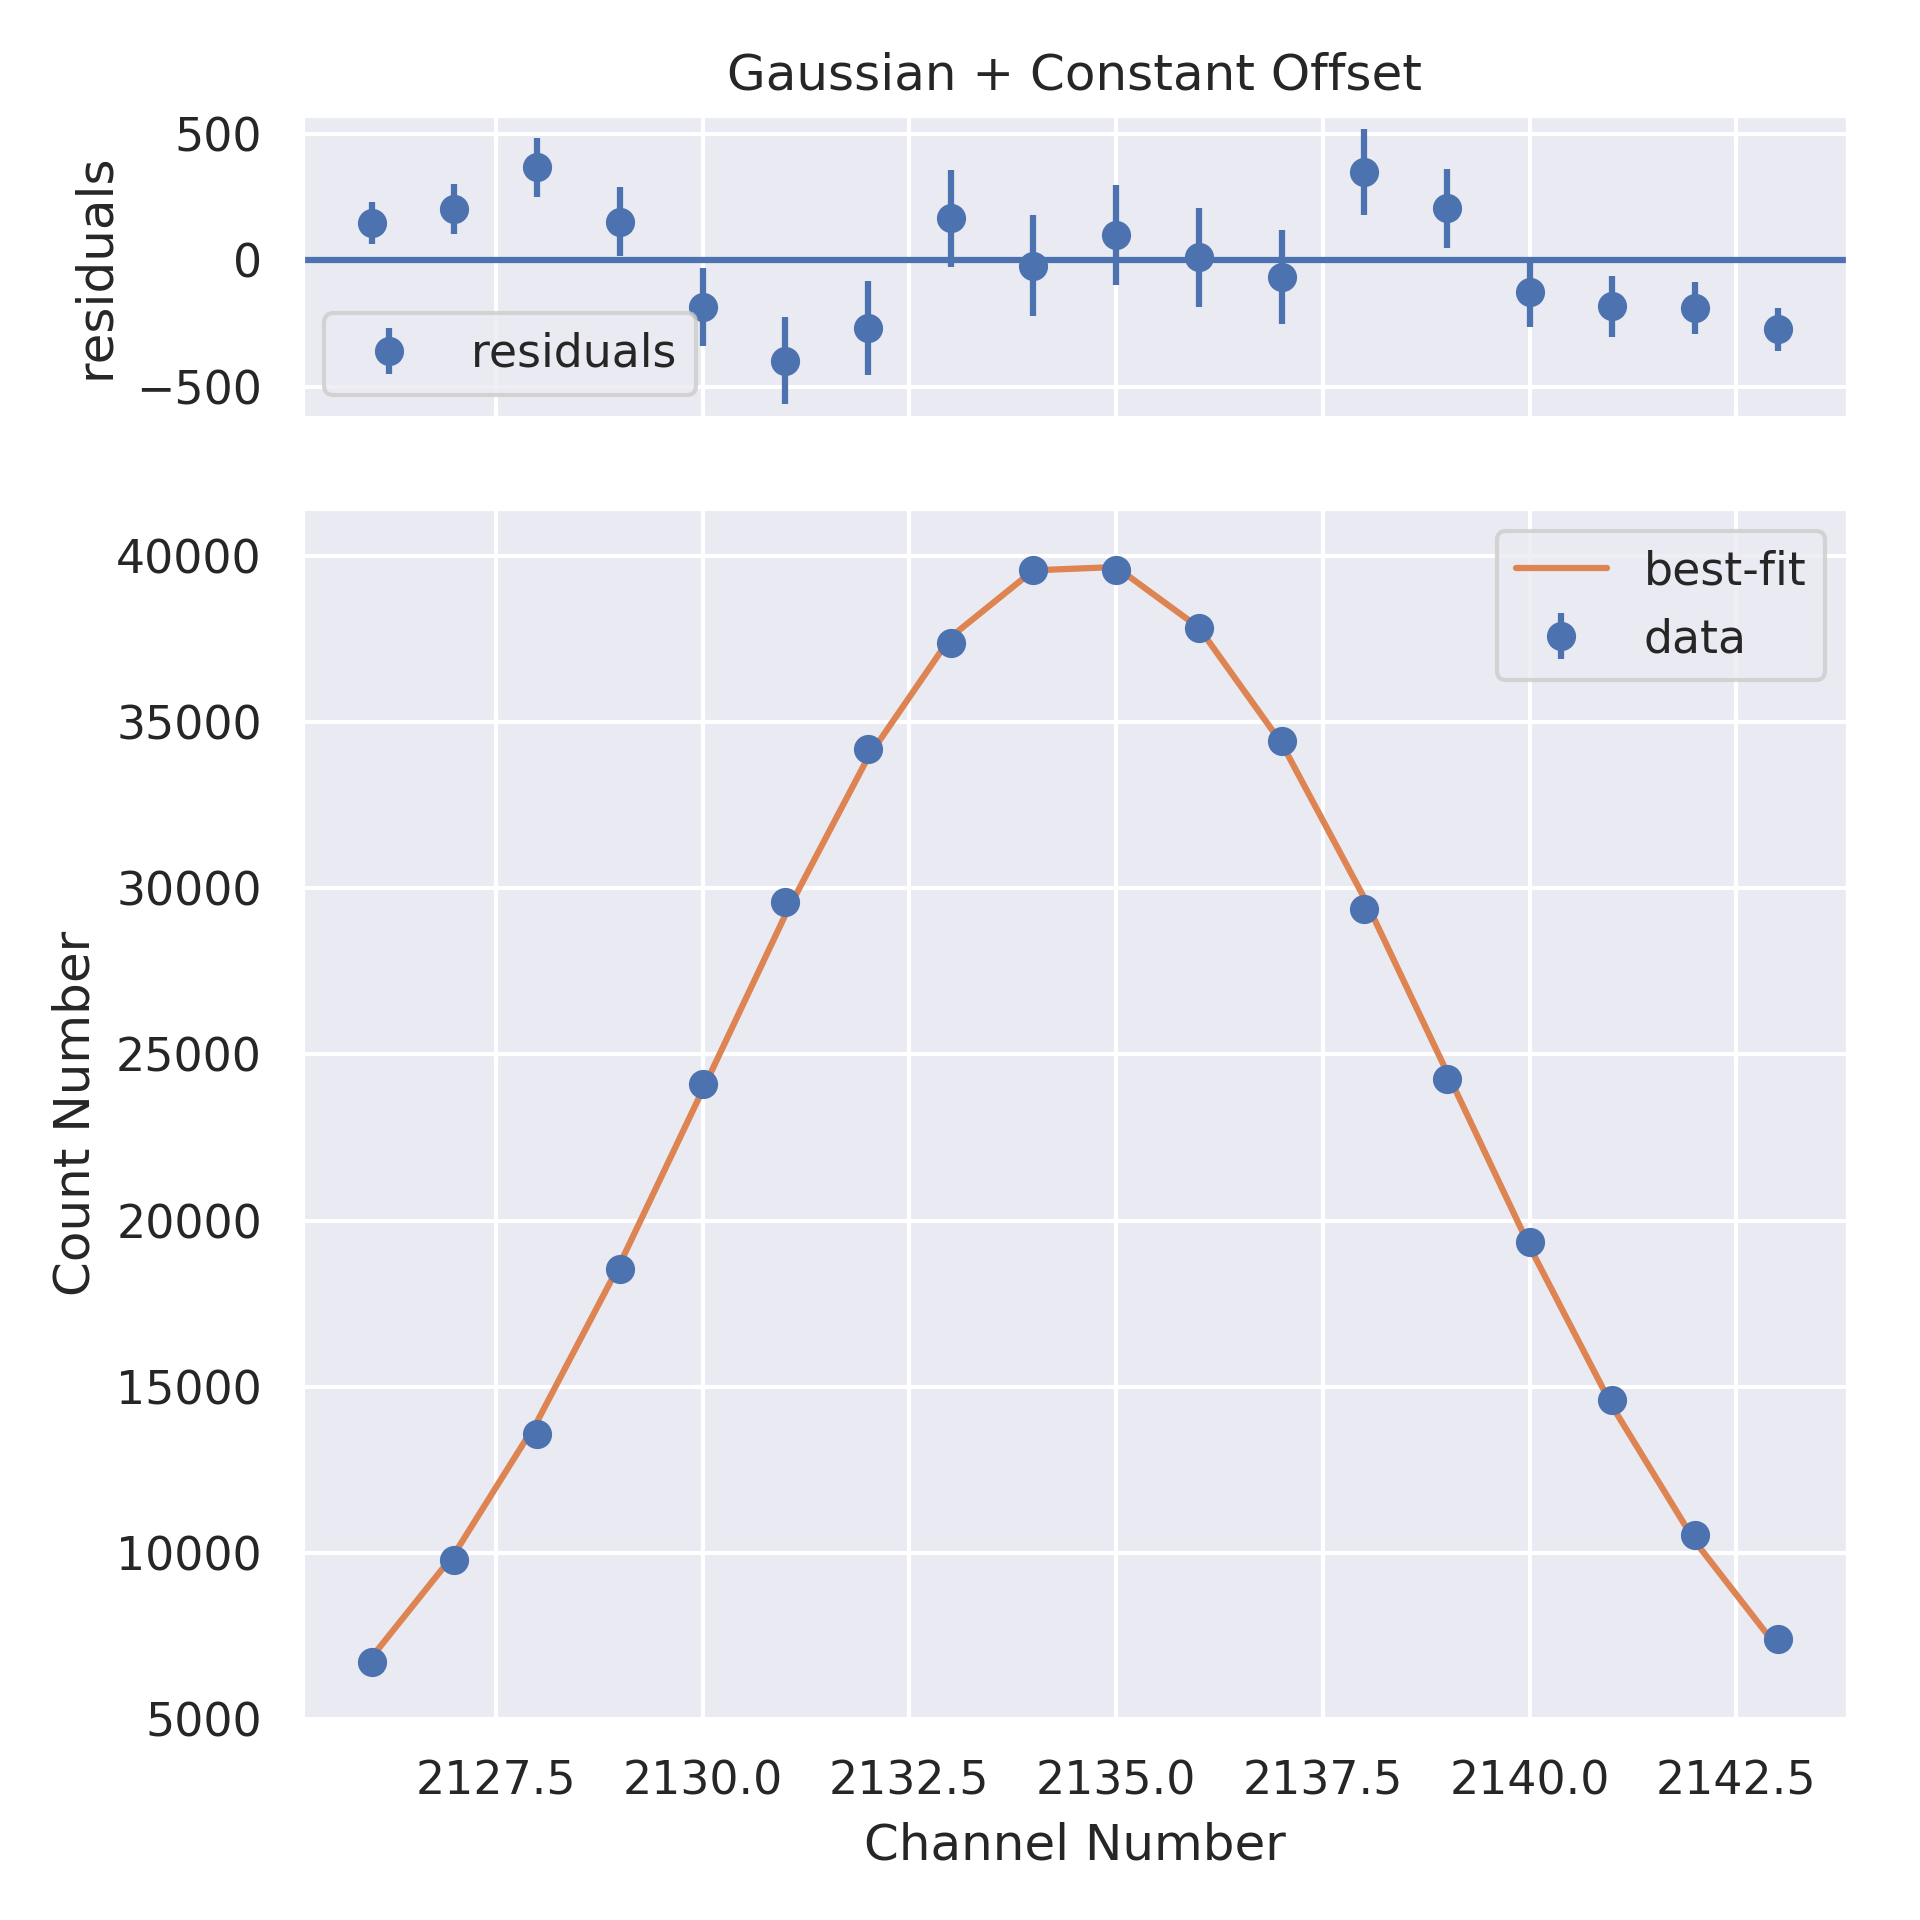
\includegraphics[width=\linewidth]{./Images/Barium133/Gauss/Gauss_5_Zoom.png}
    \caption{Zoomed in peak with fit. $\chi^2 = 51.0$, $\chi^2_\nu = 3.2$, \\ Prob = 0.02\%, $\mu = 2134.55$, $\sigma = 4.56$}
    %\label{fig:sub2}
  \end{subfigure}
  \caption{Fit of full \& zoomed in peak of \element{Ba}{133} 303 keV peak}
  %\label{fig:test}
\end{figure}
\begin{figure}[H]
  \centering
  \begin{subfigure}{.5\linewidth}
    \centering
    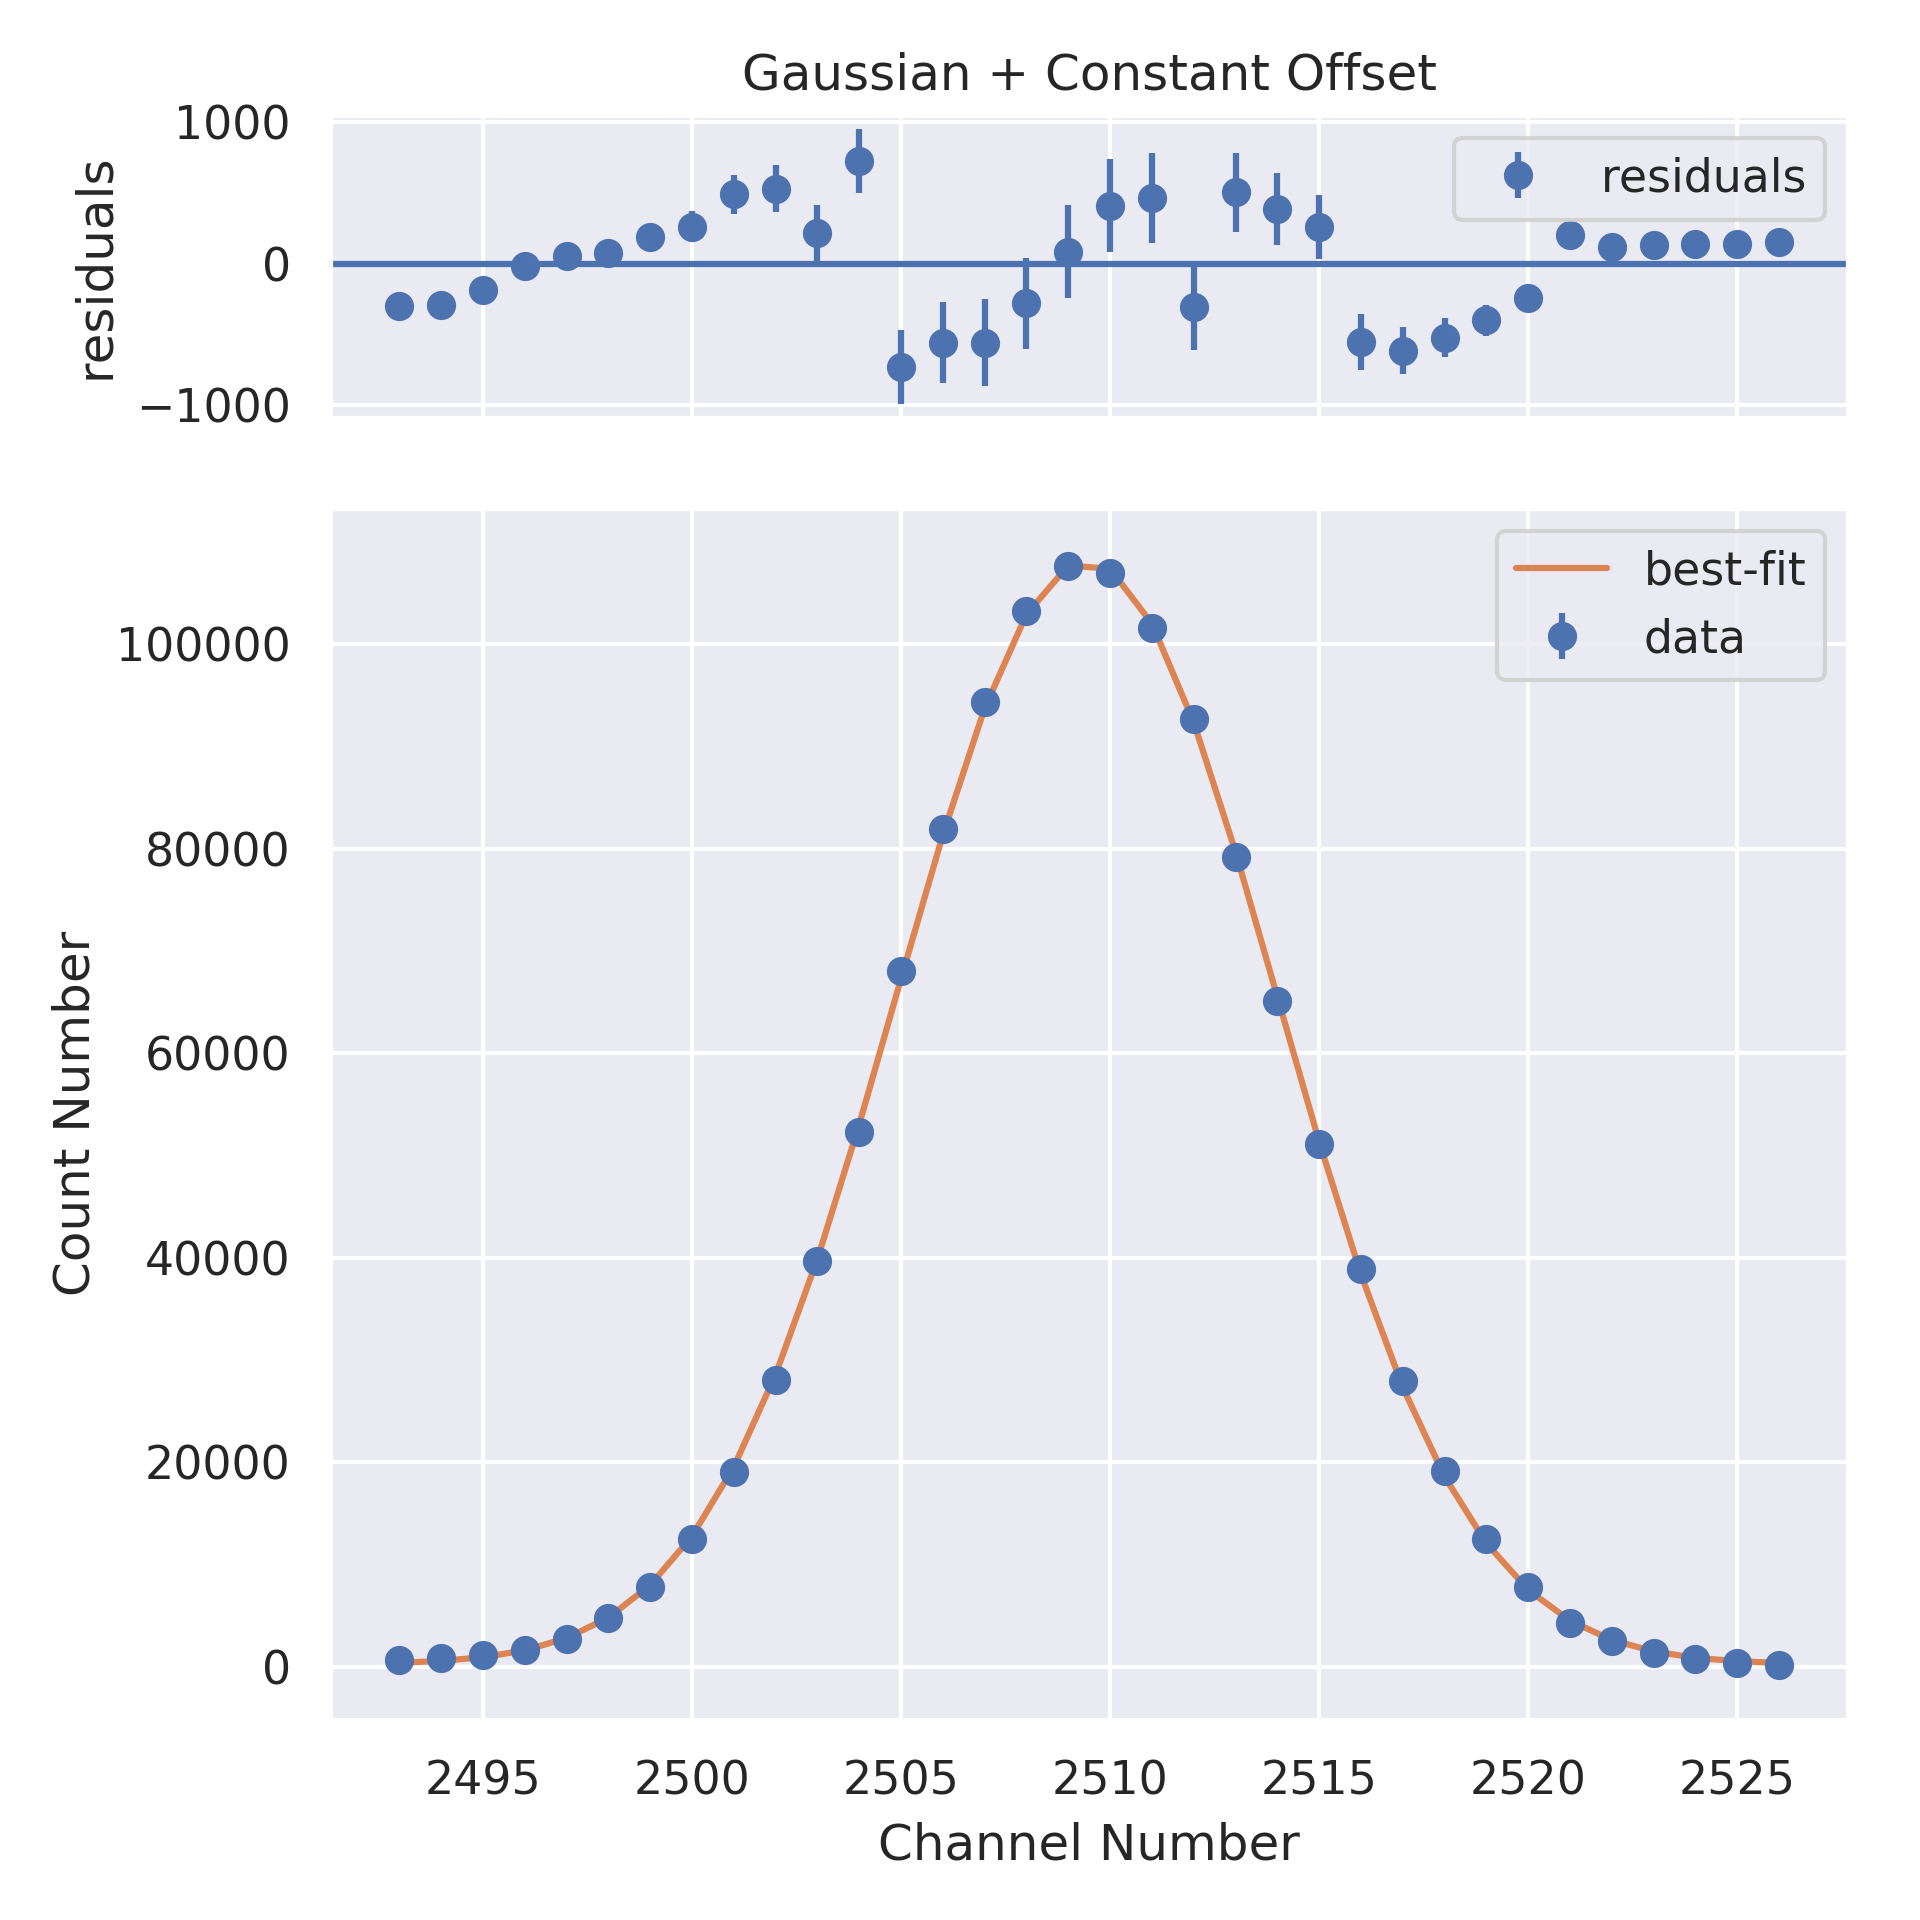
\includegraphics[width=\linewidth]{./Images/Barium133/Gauss/Gauss_6_Full.png}
    \caption{Full peak with fit. $\chi^2 = 608$, $\chi^2_\nu = 19$, \\ Prob = 0\%, $\mu = 2509.4$, $\sigma = 4.5$}
    %\label{fig:sub1}
  \end{subfigure}%
  \begin{subfigure}{.5\linewidth}
    \centering
    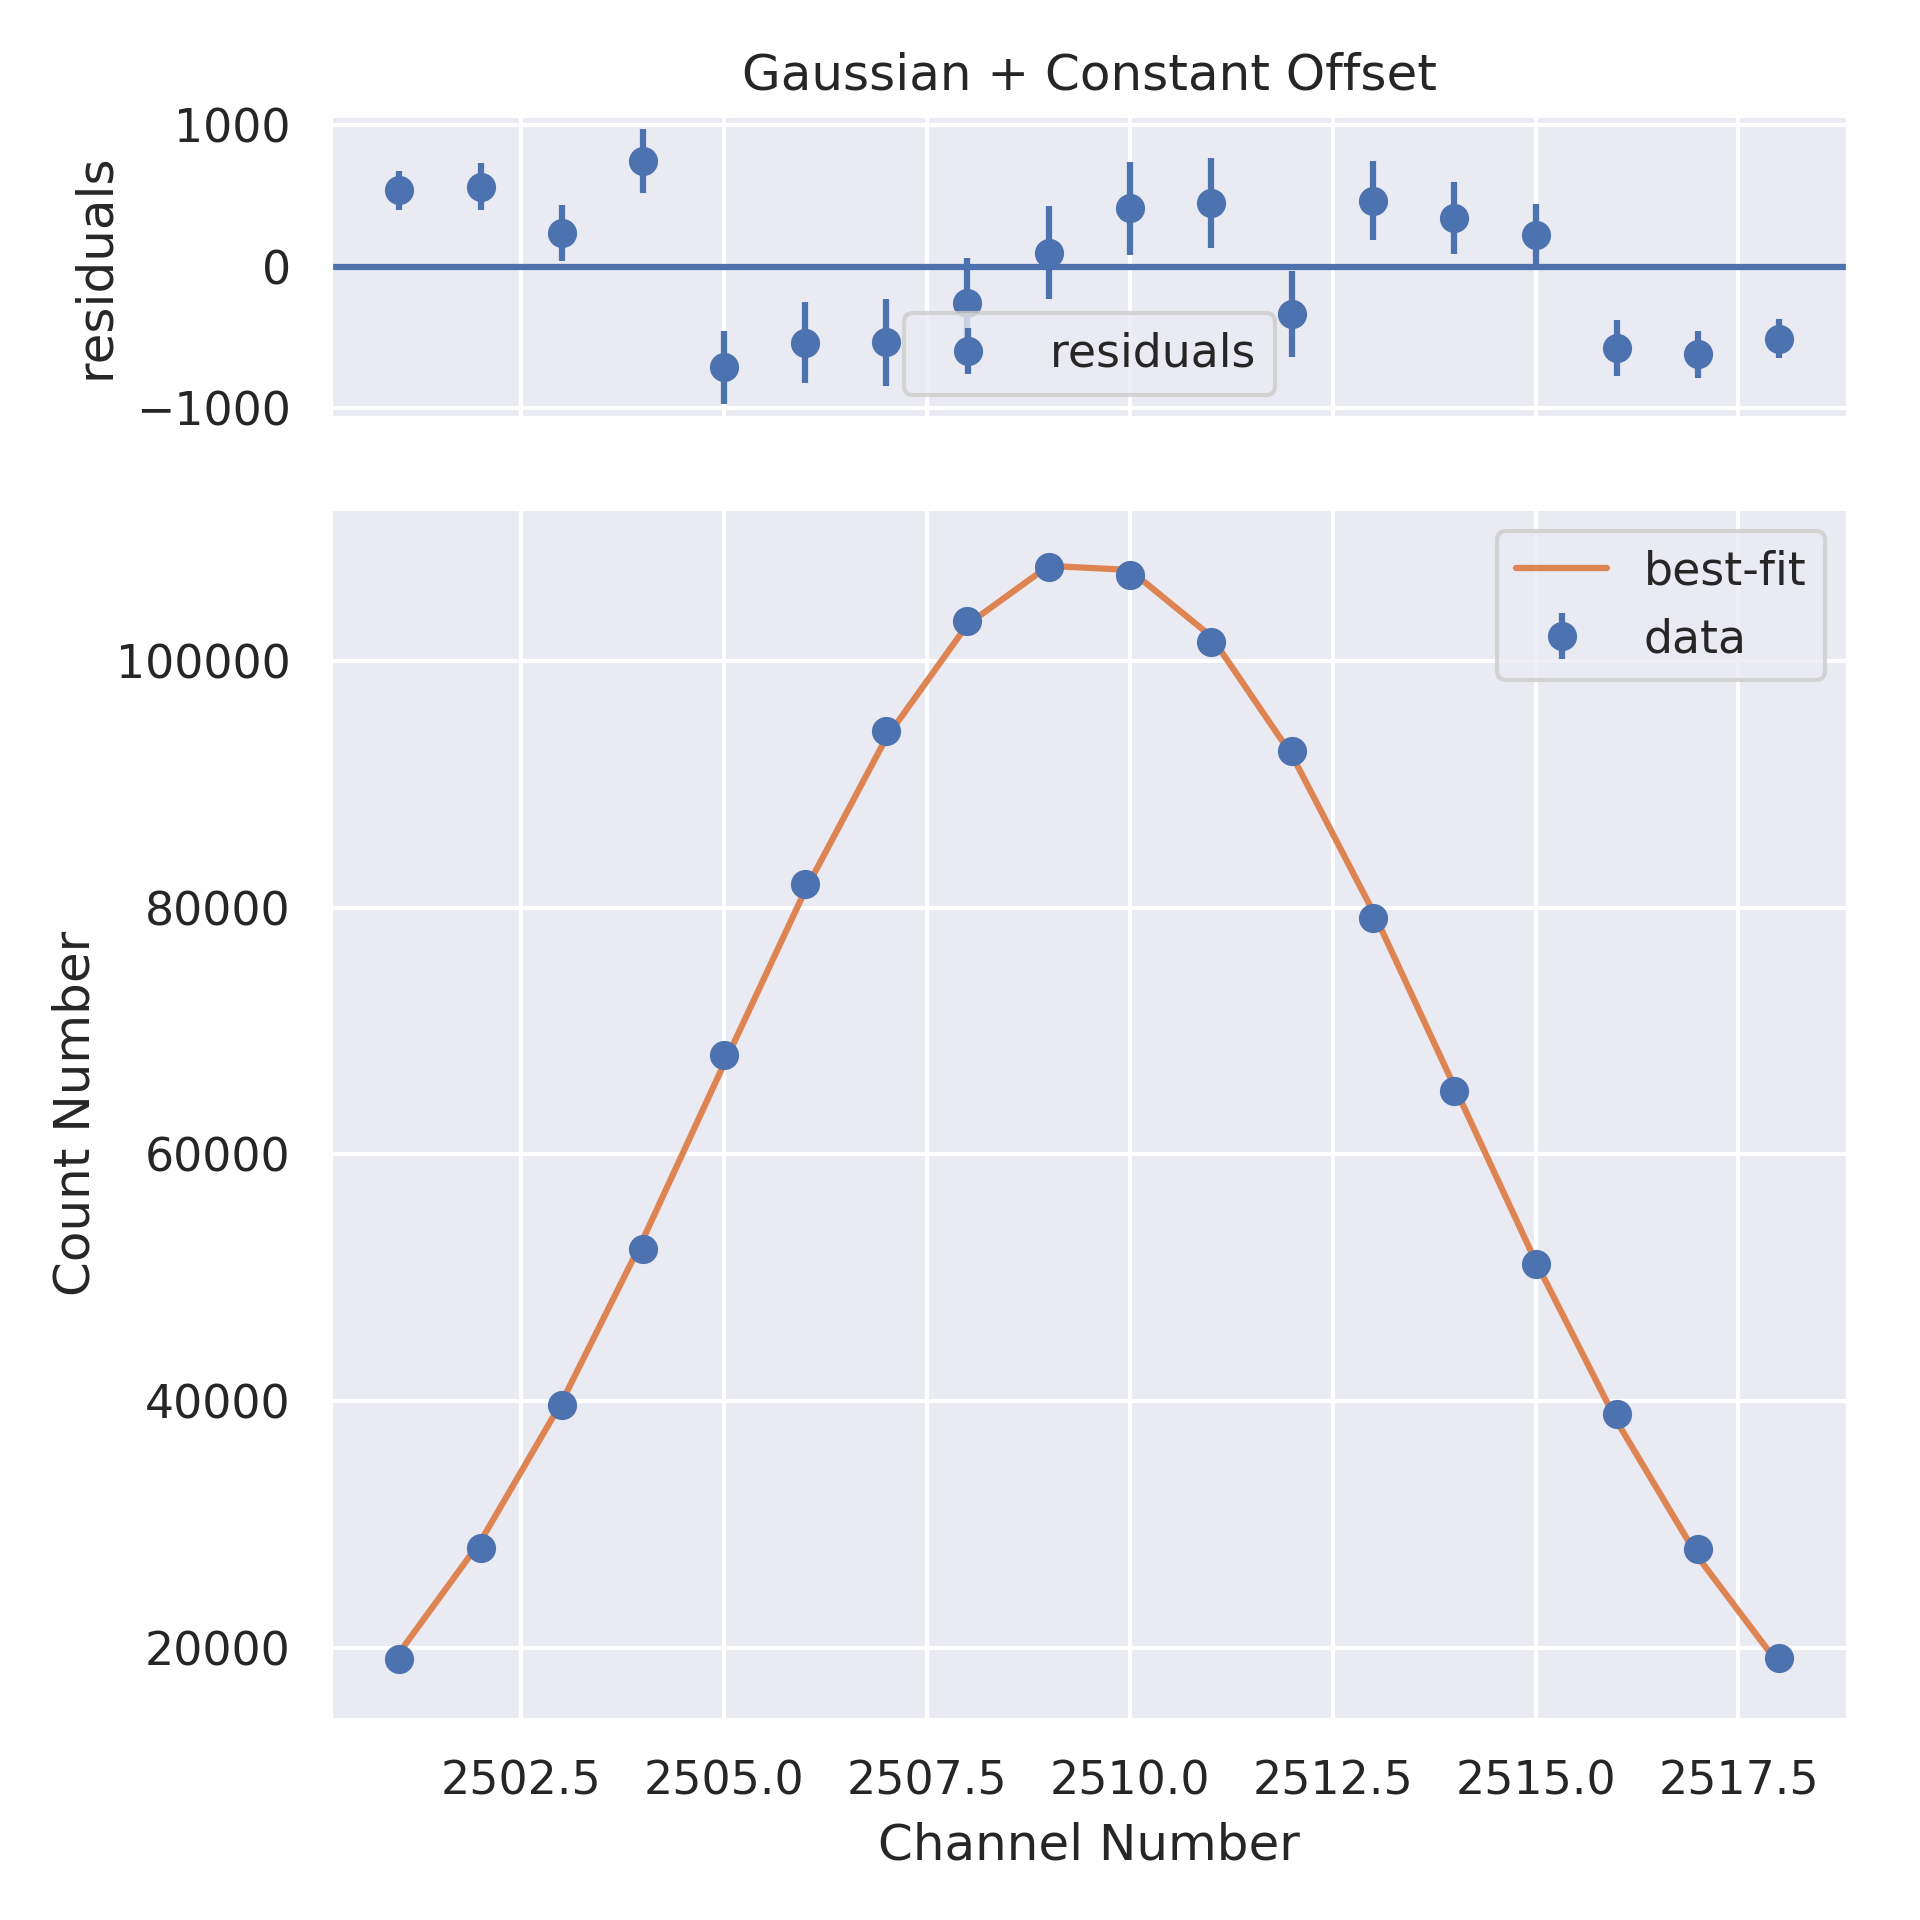
\includegraphics[width=\linewidth]{./Images/Barium133/Gauss/Gauss_6_Zoom.png}
    \caption{Zoomed in peak with fit. $\chi^2 = 100.1$, $\chi^2_\nu = 6.3$, \\ Prob = 0\%, $\mu = 2509.4$, $\sigma = 4.5$}
    %\label{fig:sub2}
  \end{subfigure}
  \caption{Fit of full \& zoomed in peak of \element{Ba}{133} 356 keV peak}
  %\label{fig:test}
\end{figure}
\begin{figure}[H]
  \centering
  \begin{subfigure}{.5\linewidth}
    \centering
    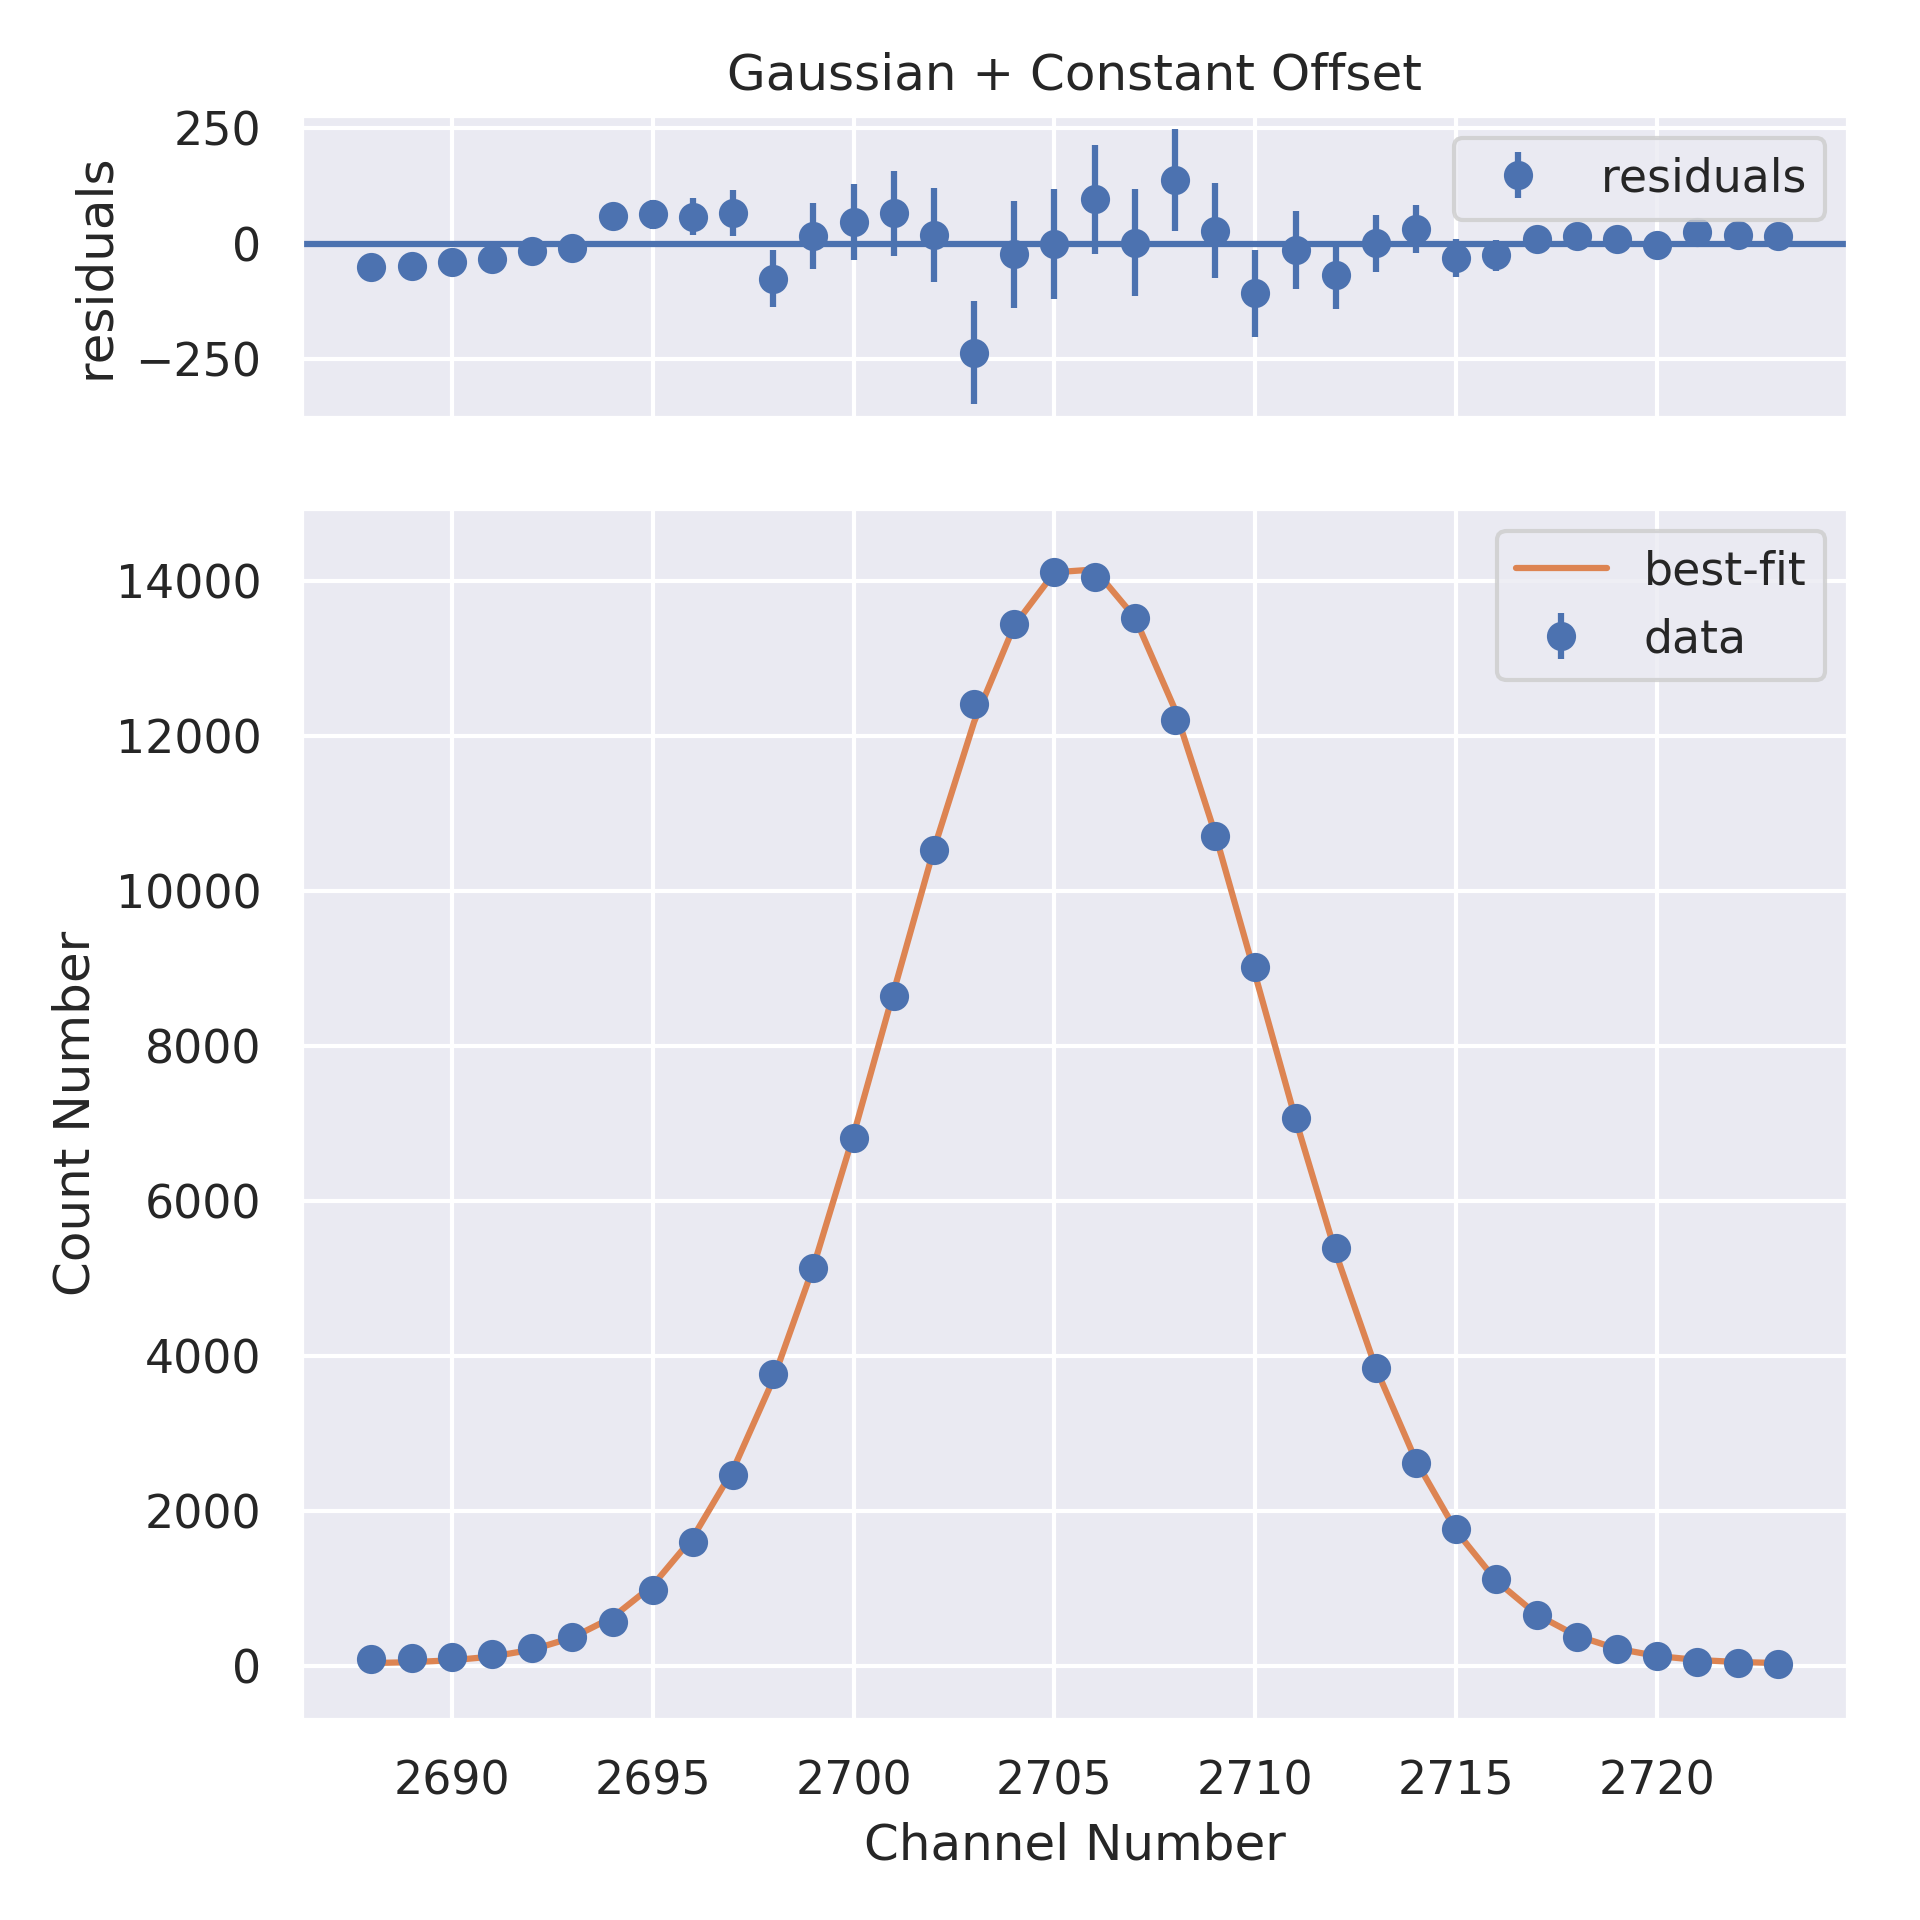
\includegraphics[width=\linewidth]{./Images/Barium133/Gauss/Gauss_7_Full.png}
    \caption{Full peak with fit. $\chi^2 = 127$, $\chi^2_\nu = 4$, \\ Prob = 0\%, $\mu = 2705.56$, $\sigma = 4.59$}
    %\label{fig:sub1}
  \end{subfigure}%
  \begin{subfigure}{.5\linewidth}
    \centering
    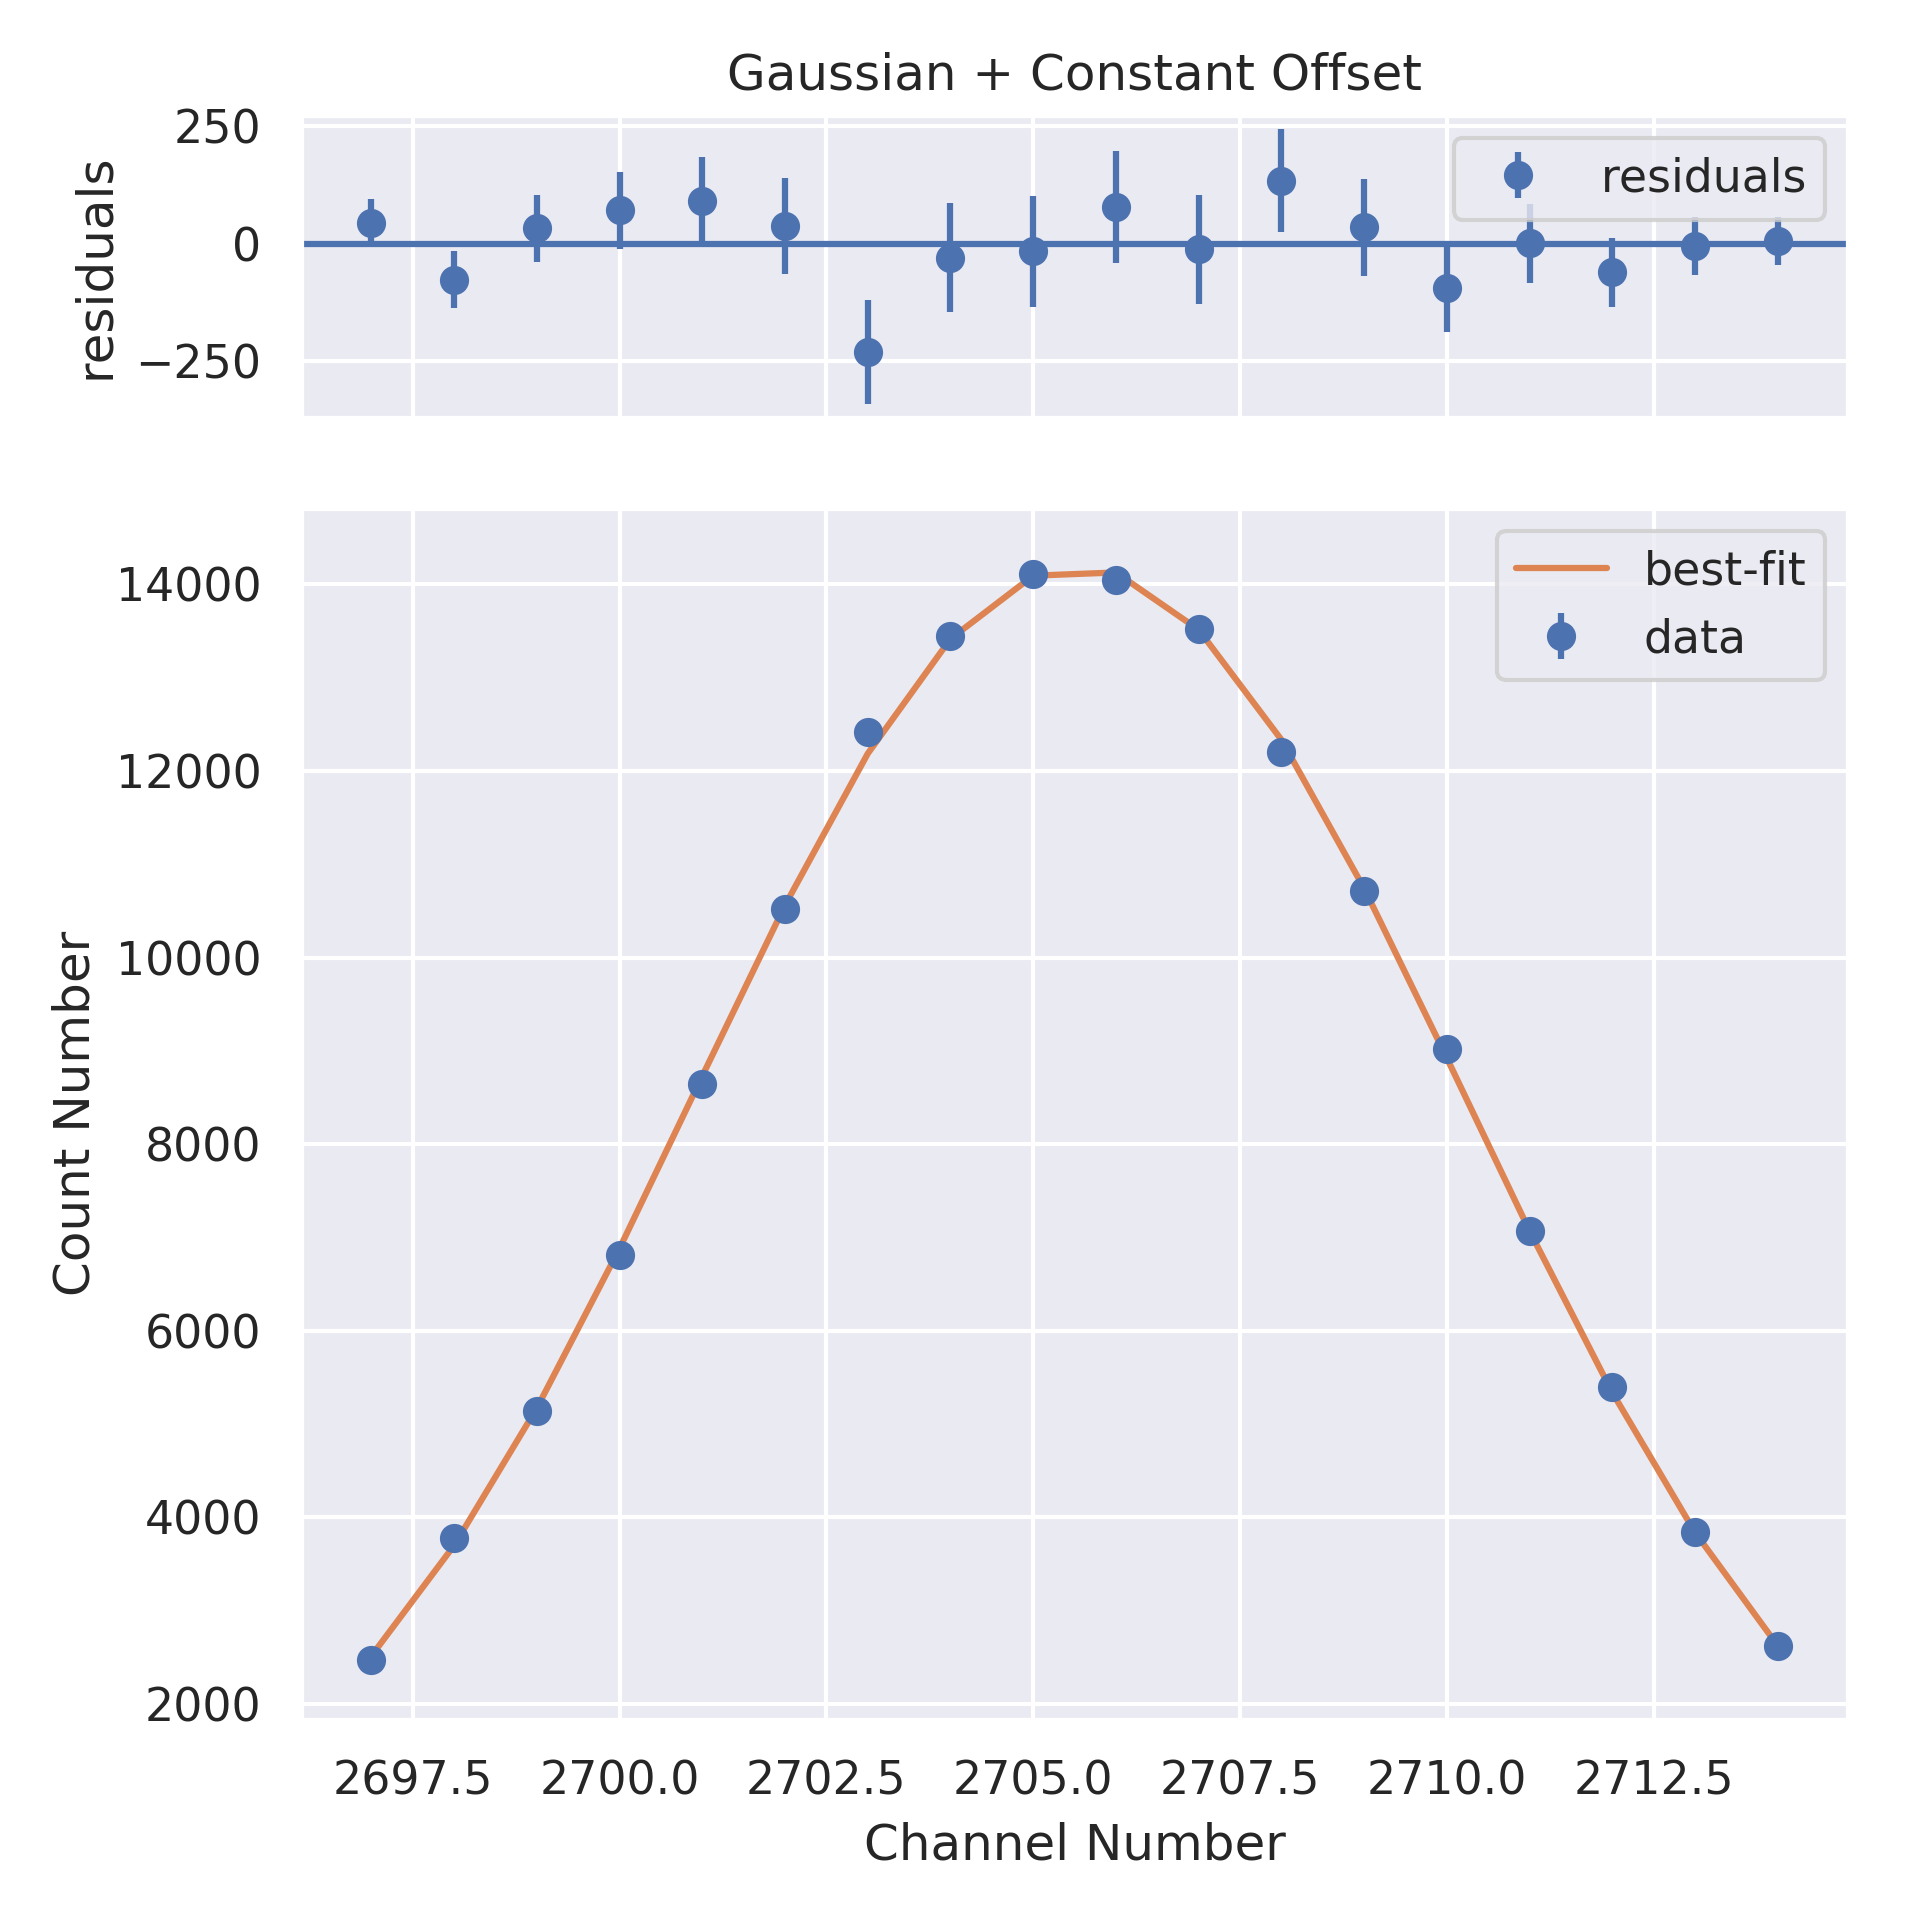
\includegraphics[width=\linewidth]{./Images/Barium133/Gauss/Gauss_7_Zoom.png}
    \caption{Zoomed in peak with fit. $\chi^2 = 12.5$, $\chi^2_\nu = 0.8$, \\ Prob = 70.9\%, $\mu = 2705.55$, $\sigma = 4.64$}
    %\label{fig:sub2}
  \end{subfigure}
  \caption{Fit of full \& zoomed in peak of \element{Ba}{133} 384 keV peak}
  %\label{fig:test}
\end{figure}
\clearpage
\subsubsection{Gaussian + Linear Fit}
\begin{figure}[H]
  \centering
  \begin{subfigure}{.5\linewidth}
    \centering
    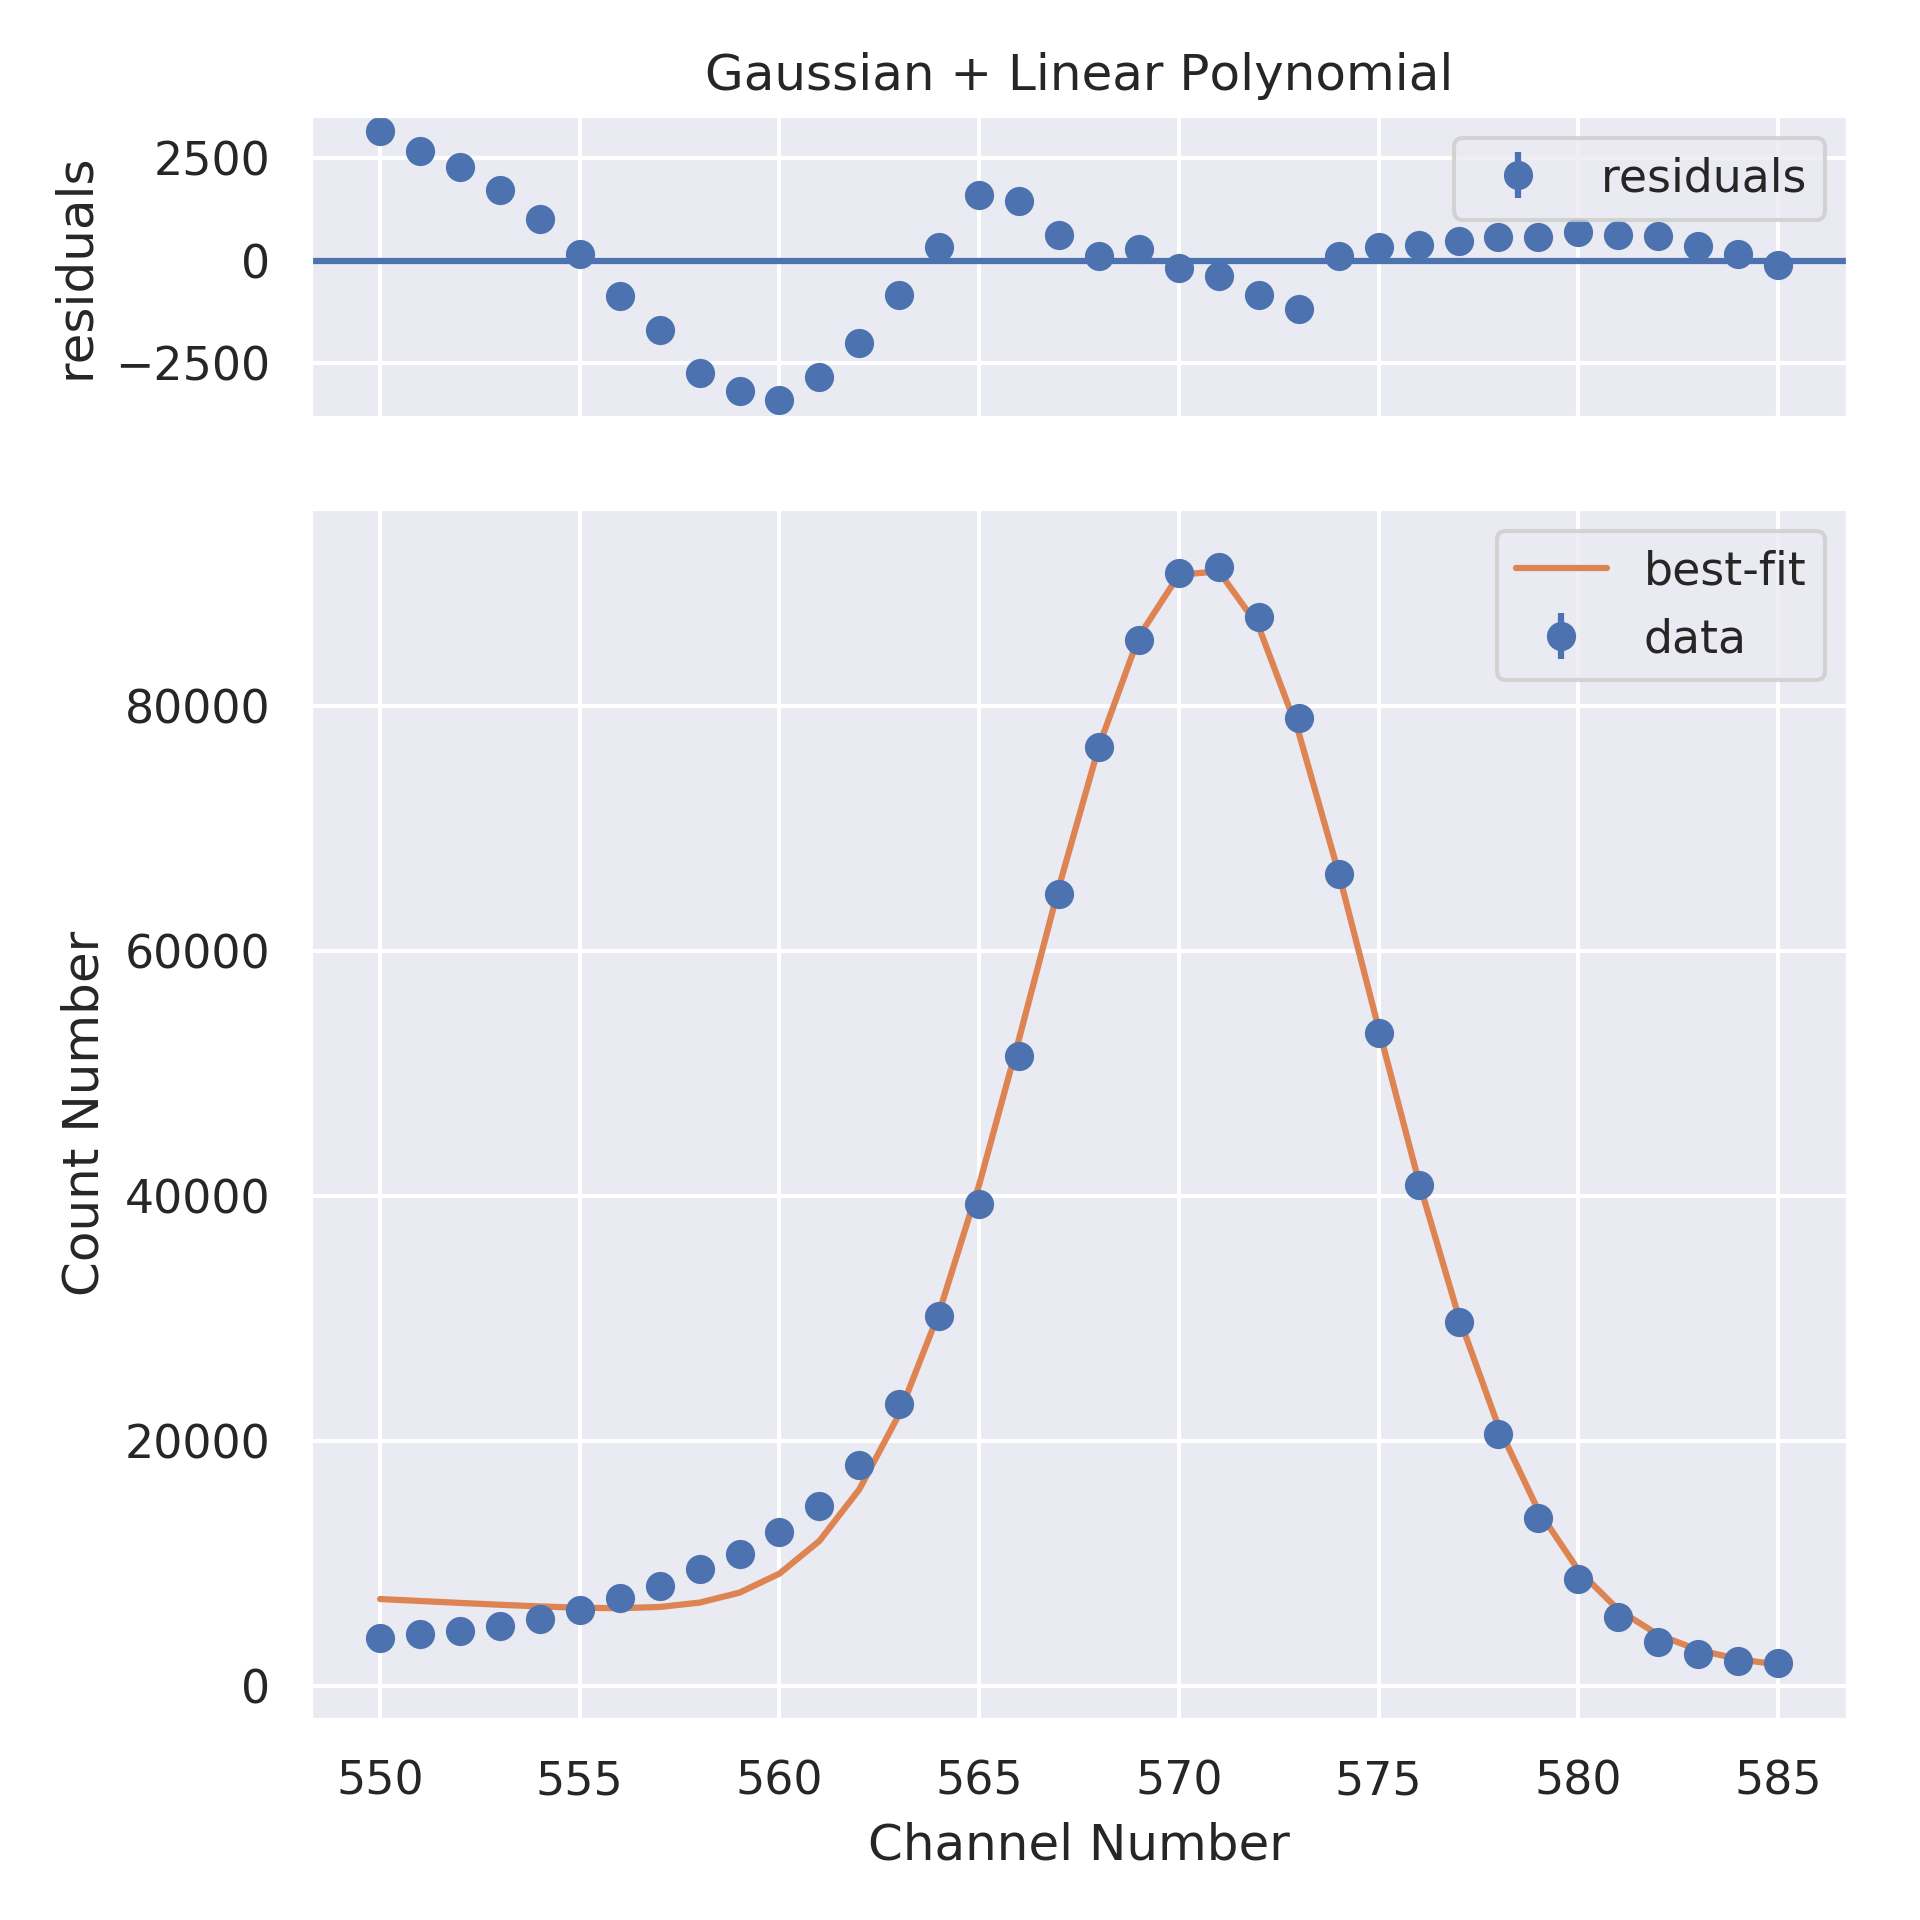
\includegraphics[width=\linewidth]{./Images/Barium133/Linear/Linear_1_Full.png}
    \caption{Full peak with fit. $\chi^2 = 10435$, $\chi^2_\nu = 307$, \\ Prob = 0\%, $\mu = 570.59$, $\sigma = 4.20$}
    %\label{fig:sub1}
  \end{subfigure}%
  \begin{subfigure}{.5\linewidth}
    \centering
    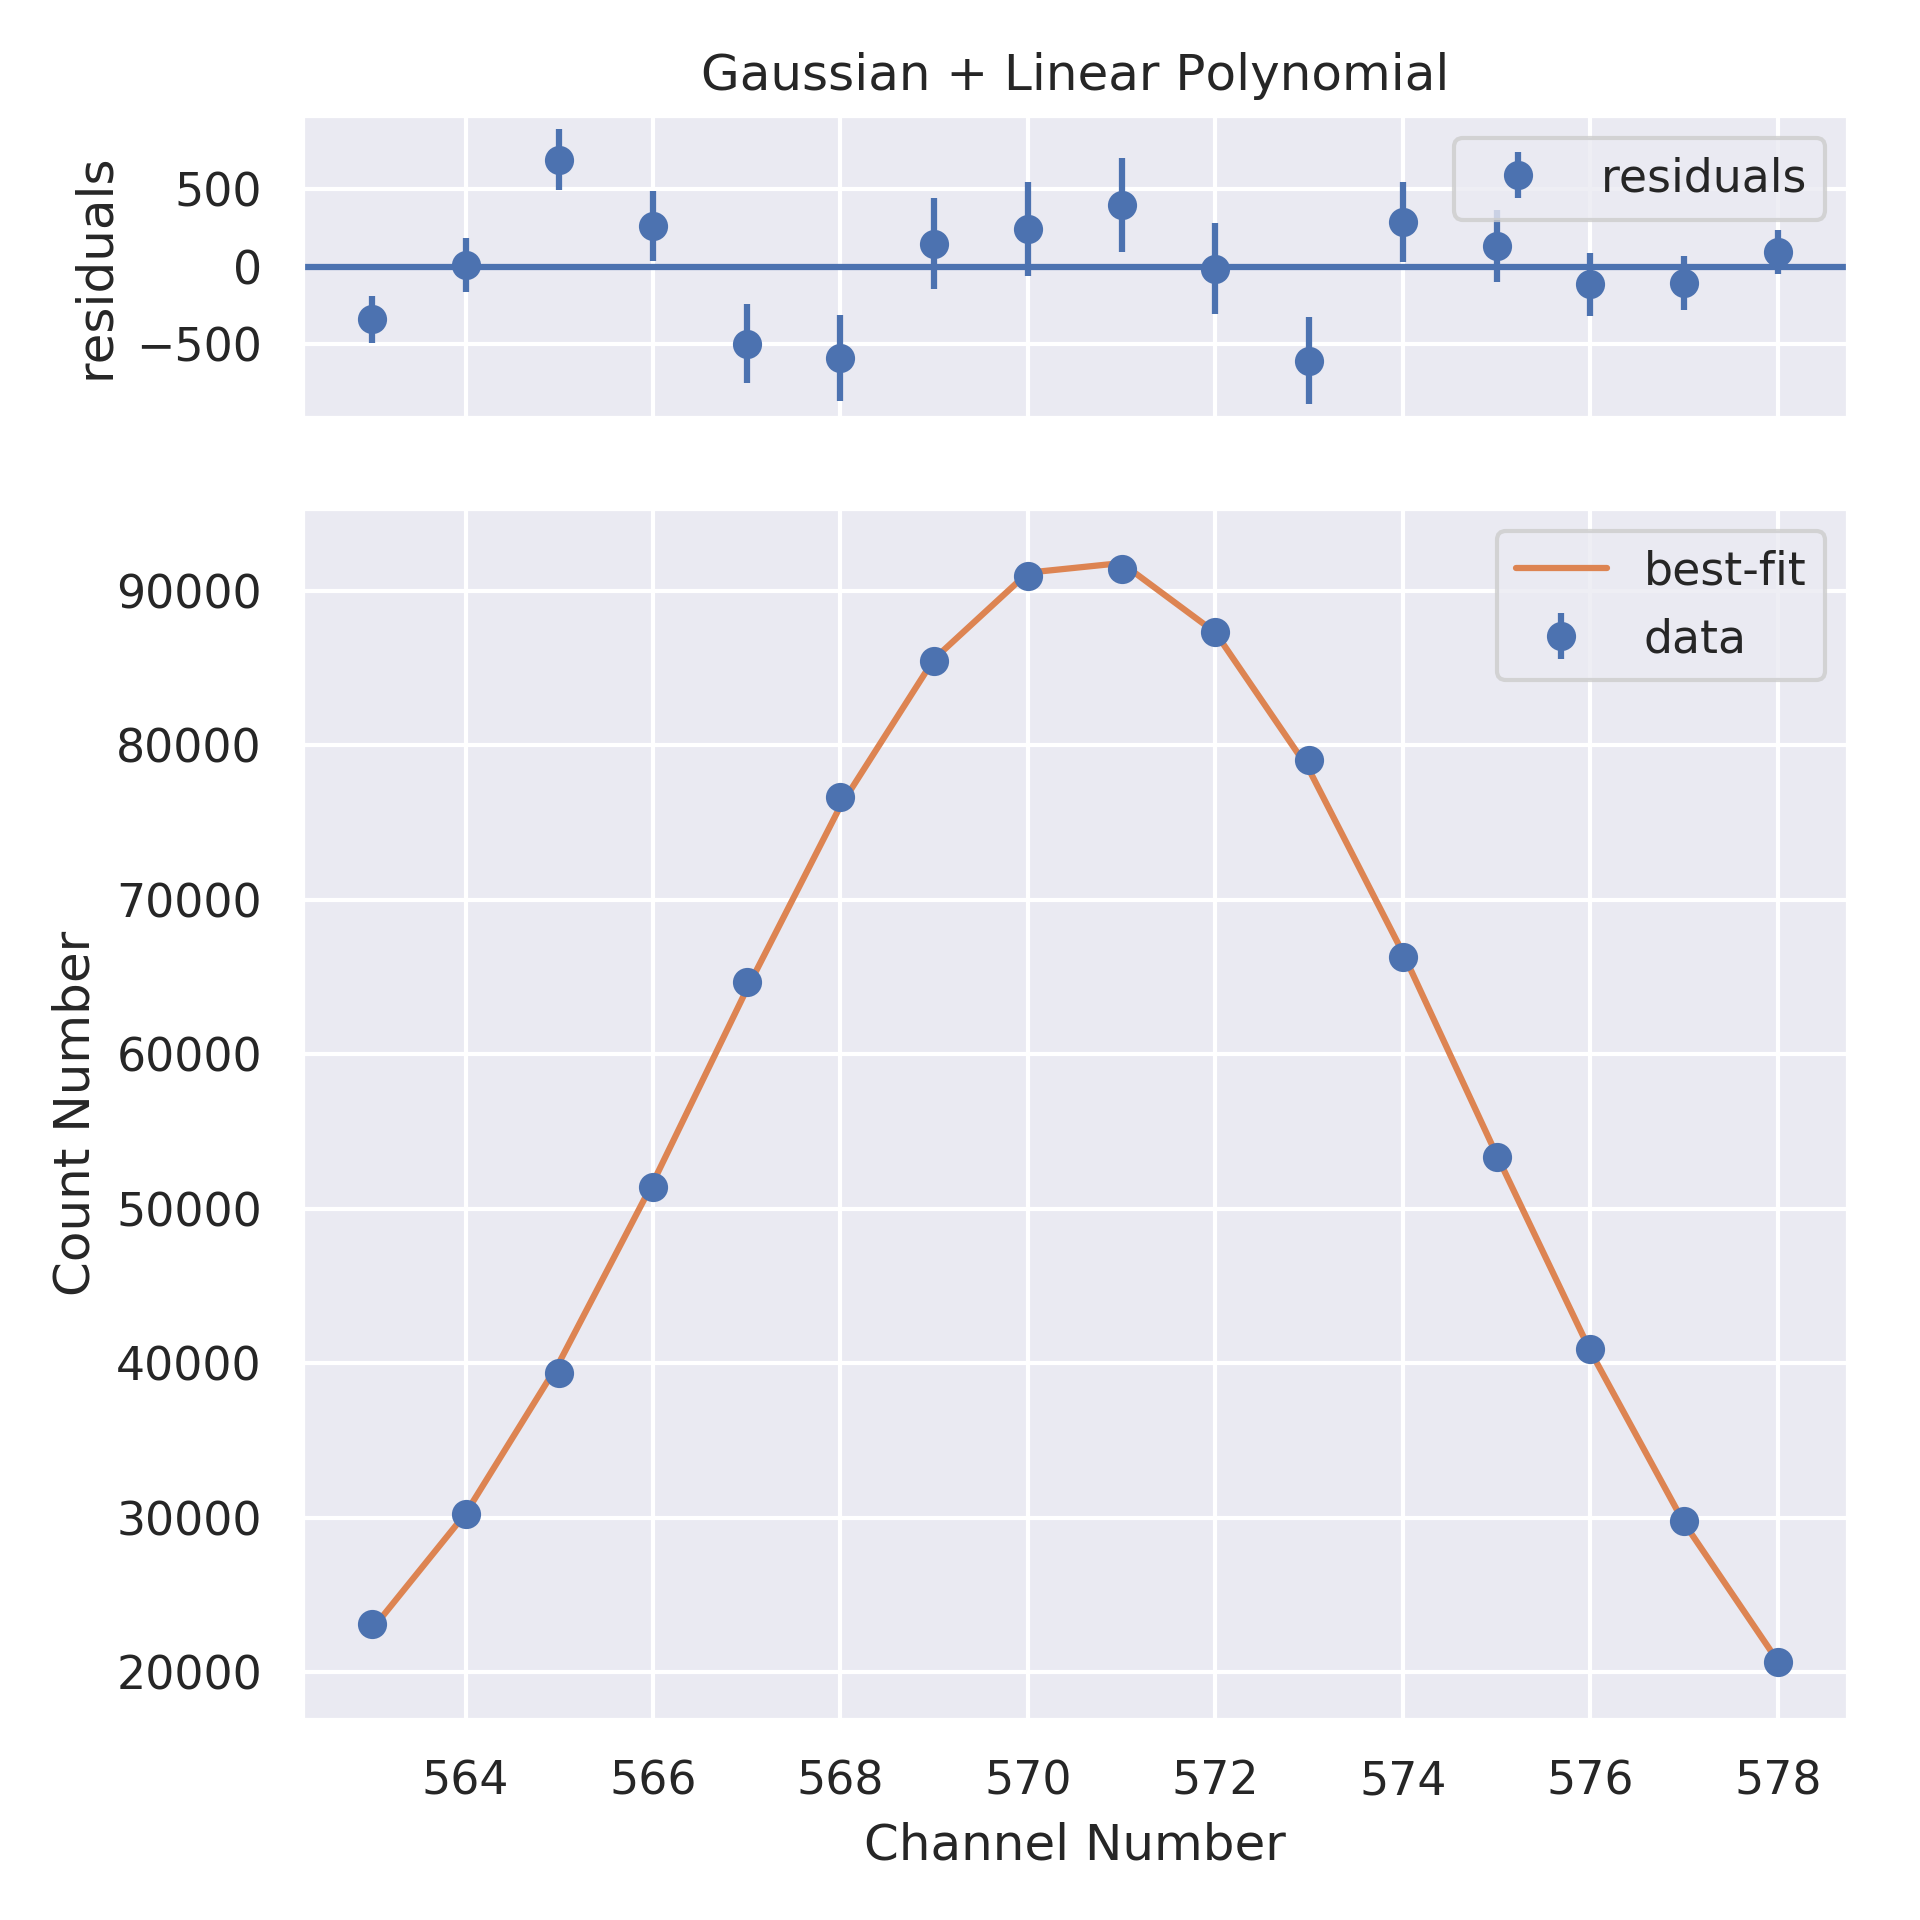
\includegraphics[width=\linewidth]{./Images/Barium133/Linear/Linear_1_Zoom.png}
    \caption{Zoomed in peak with fit. $\chi^2 = 36.6$, $\chi^2_\nu = 2.6$, \\ Prob = 0.08\%, $\mu = 570.68$, $\sigma = 4.05$}
    %\label{fig:sub2}
  \end{subfigure}
  \caption{Fit of full \& zoomed in peak of \element{Ba}{133} 81 keV peak}
  %\label{fig:test}
\end{figure}
\begin{figure}[H]
  \centering
  \begin{subfigure}{.5\linewidth}
    \centering
    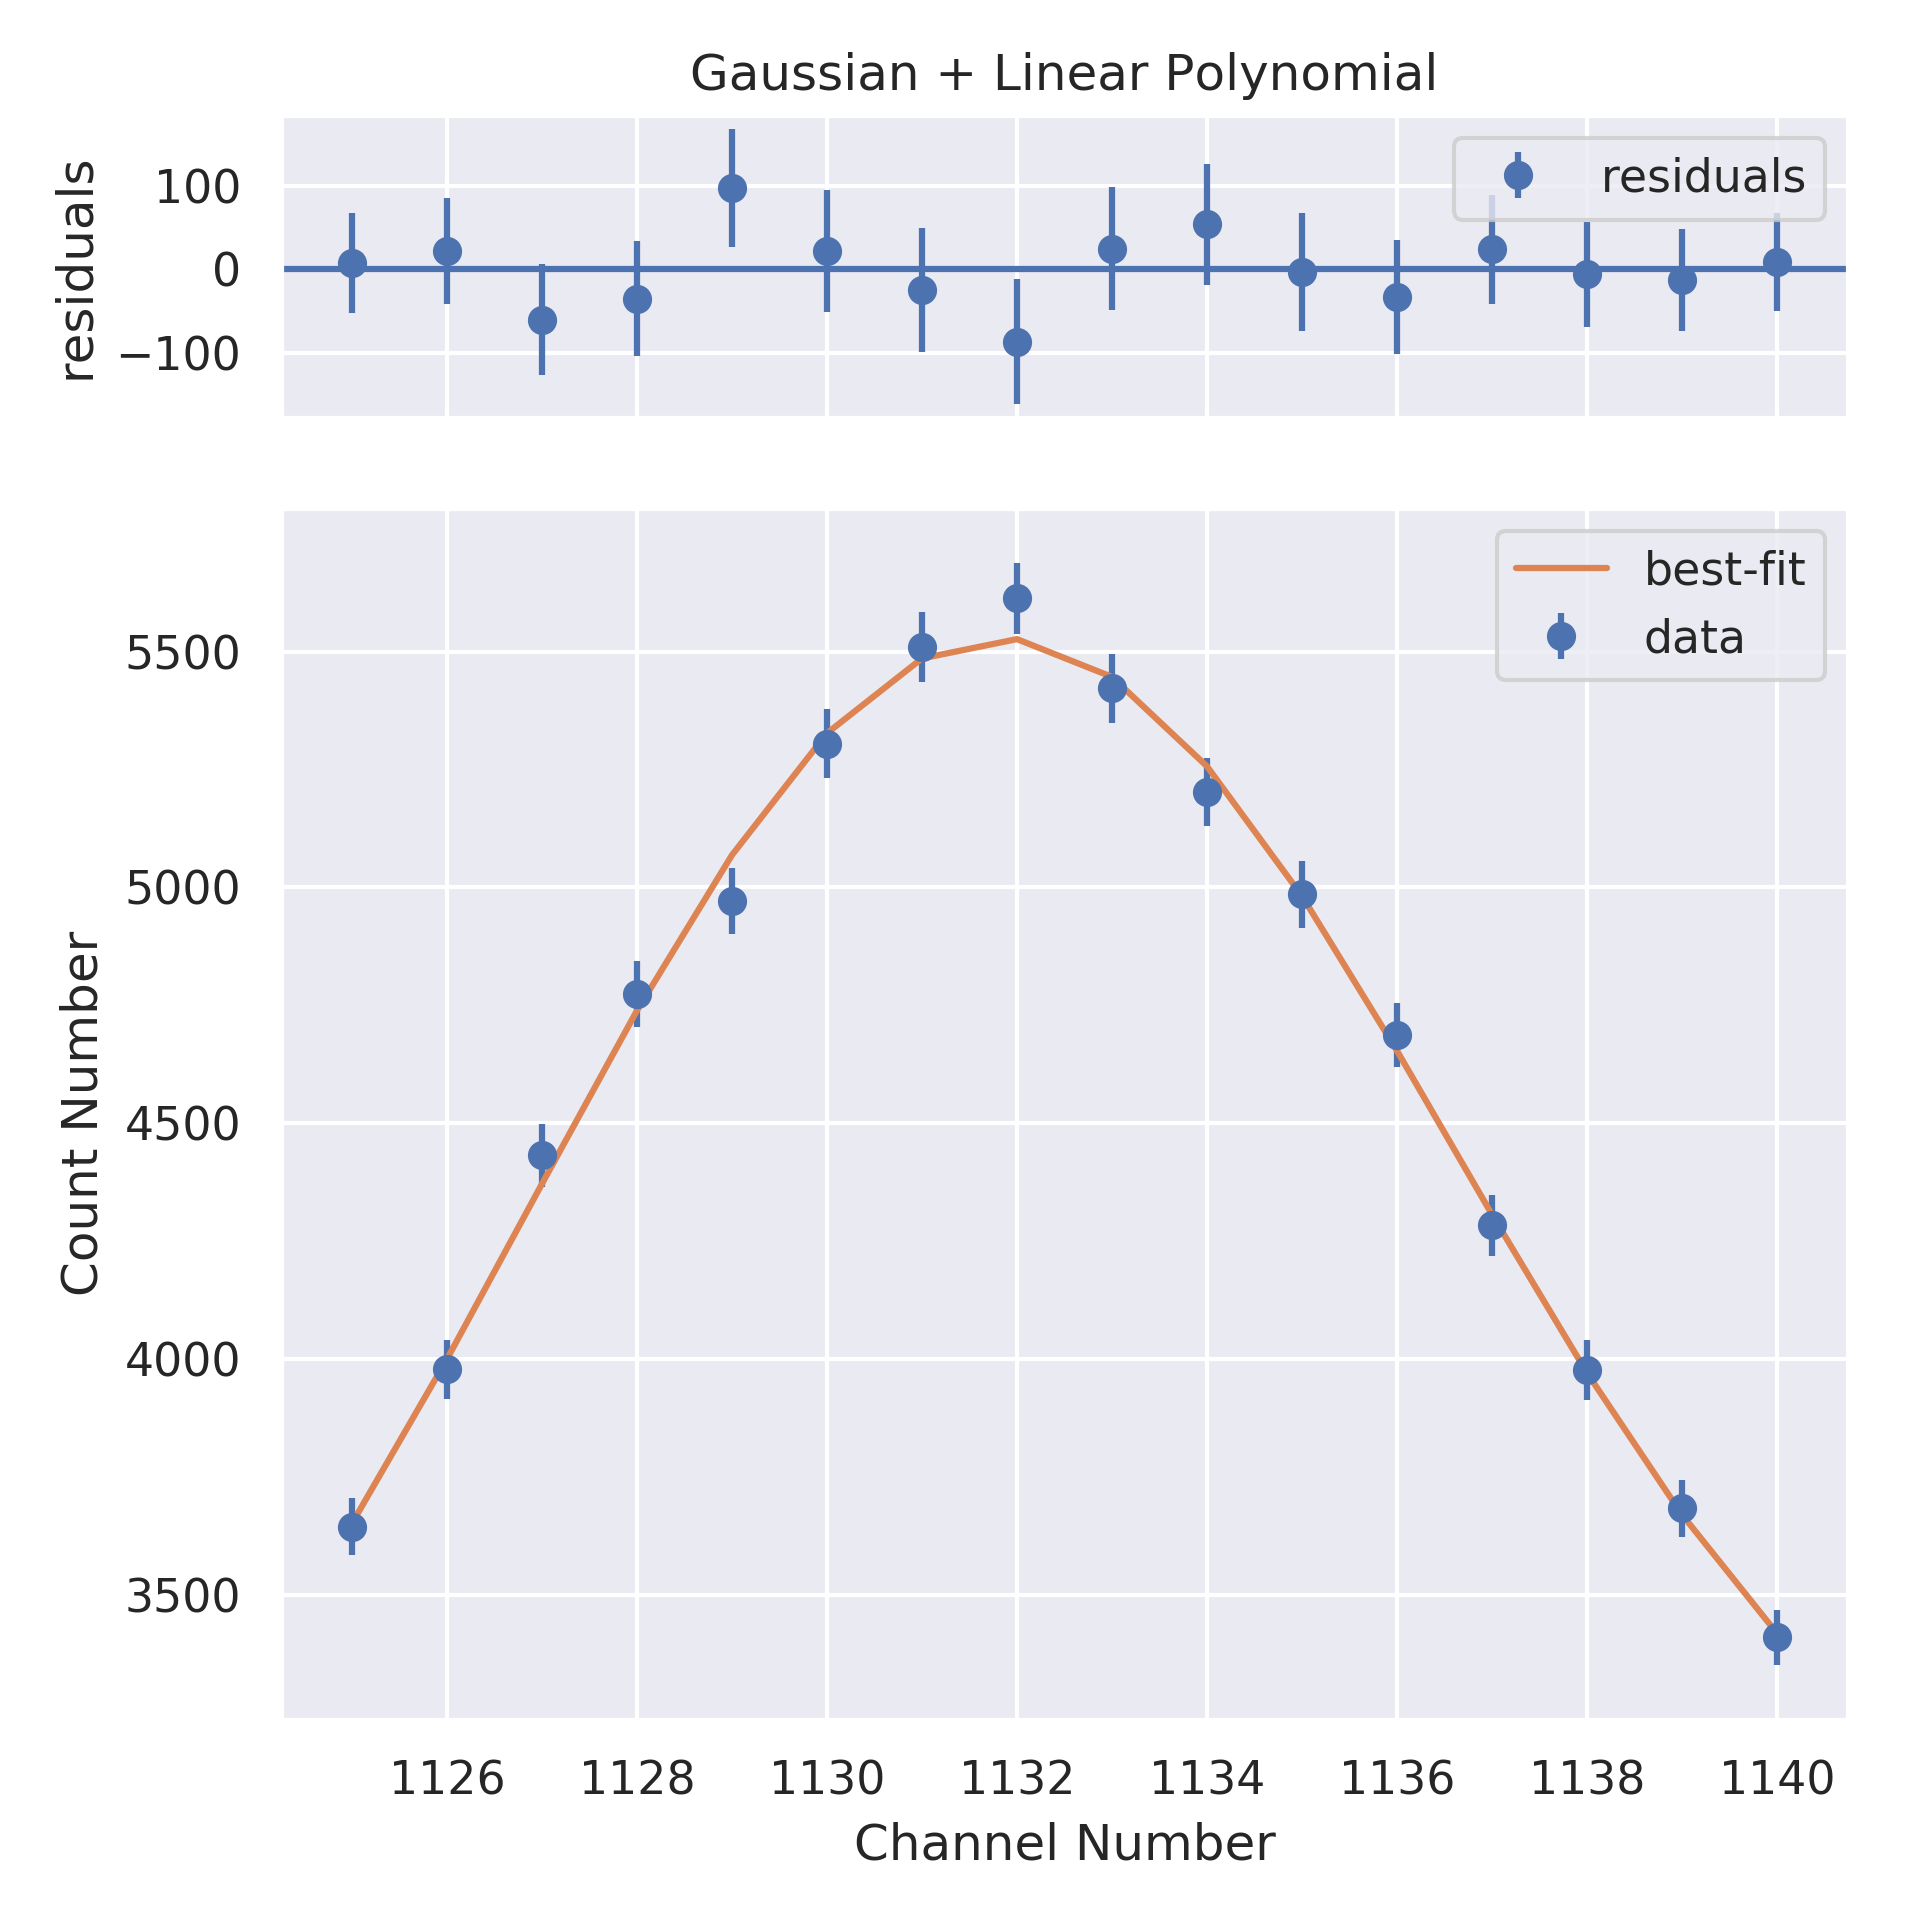
\includegraphics[width=\linewidth]{./Images/Barium133/Linear/Linear_2_Full.png}
    \caption{Full peak with fit. $\chi^2 = 5.78$, $\chi^2_\nu = 0.41$, \\ Prob = 97.18\%, $\mu = 1131.73$, $\sigma = 4.85$}
    %\label{fig:sub1}
  \end{subfigure}%
  \begin{subfigure}{.5\linewidth}
    \centering
    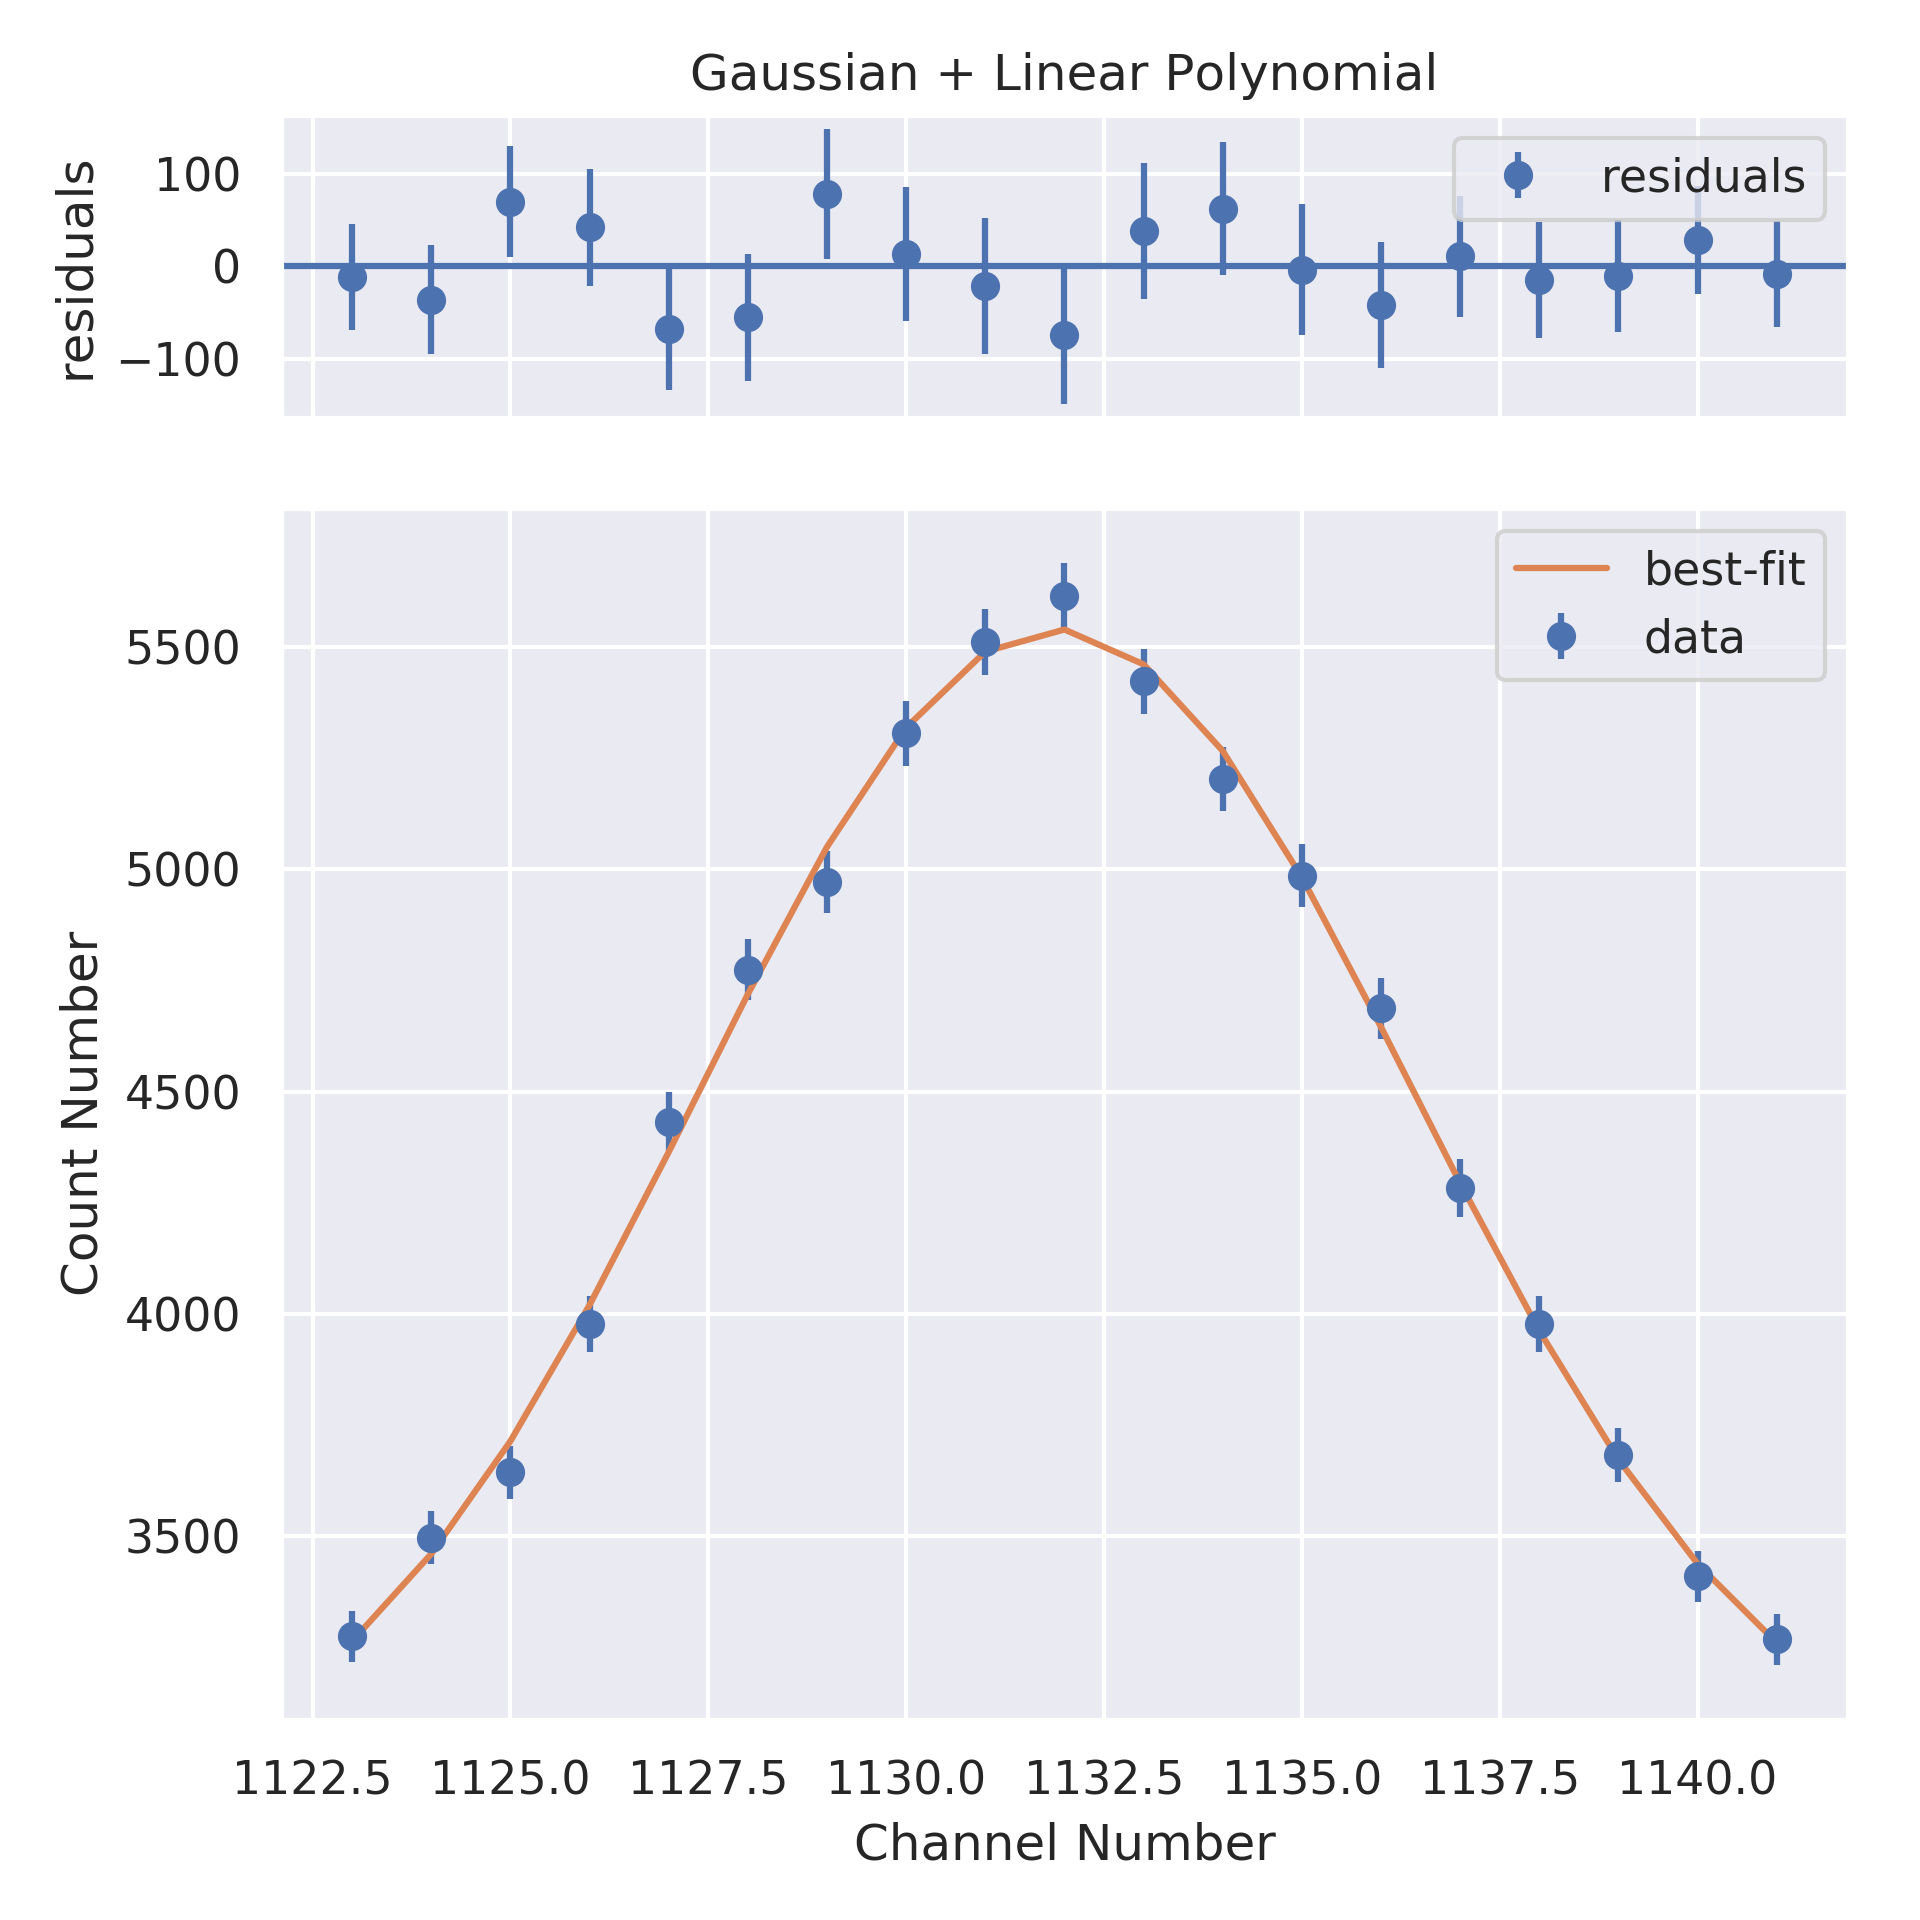
\includegraphics[width=\linewidth]{./Images/Barium133/Linear/Linear_2_Zoom.png}
    \caption{Zoomed in peak with fit. $\chi^2 = 8.02$, $\chi^2_\nu = 0.47$, \\ Prob = 96.61\%, $\mu = 1131.87$, $\sigma = 4.51$}
    %\label{fig:sub2}
  \end{subfigure}
  \caption{Fit of full \& zoomed in peak of \element{Ba}{133} 161 keV peak}
  %\label{fig:test}
\end{figure}
\begin{figure}[H]
  \centering
  \begin{subfigure}{.5\linewidth}
    \centering
    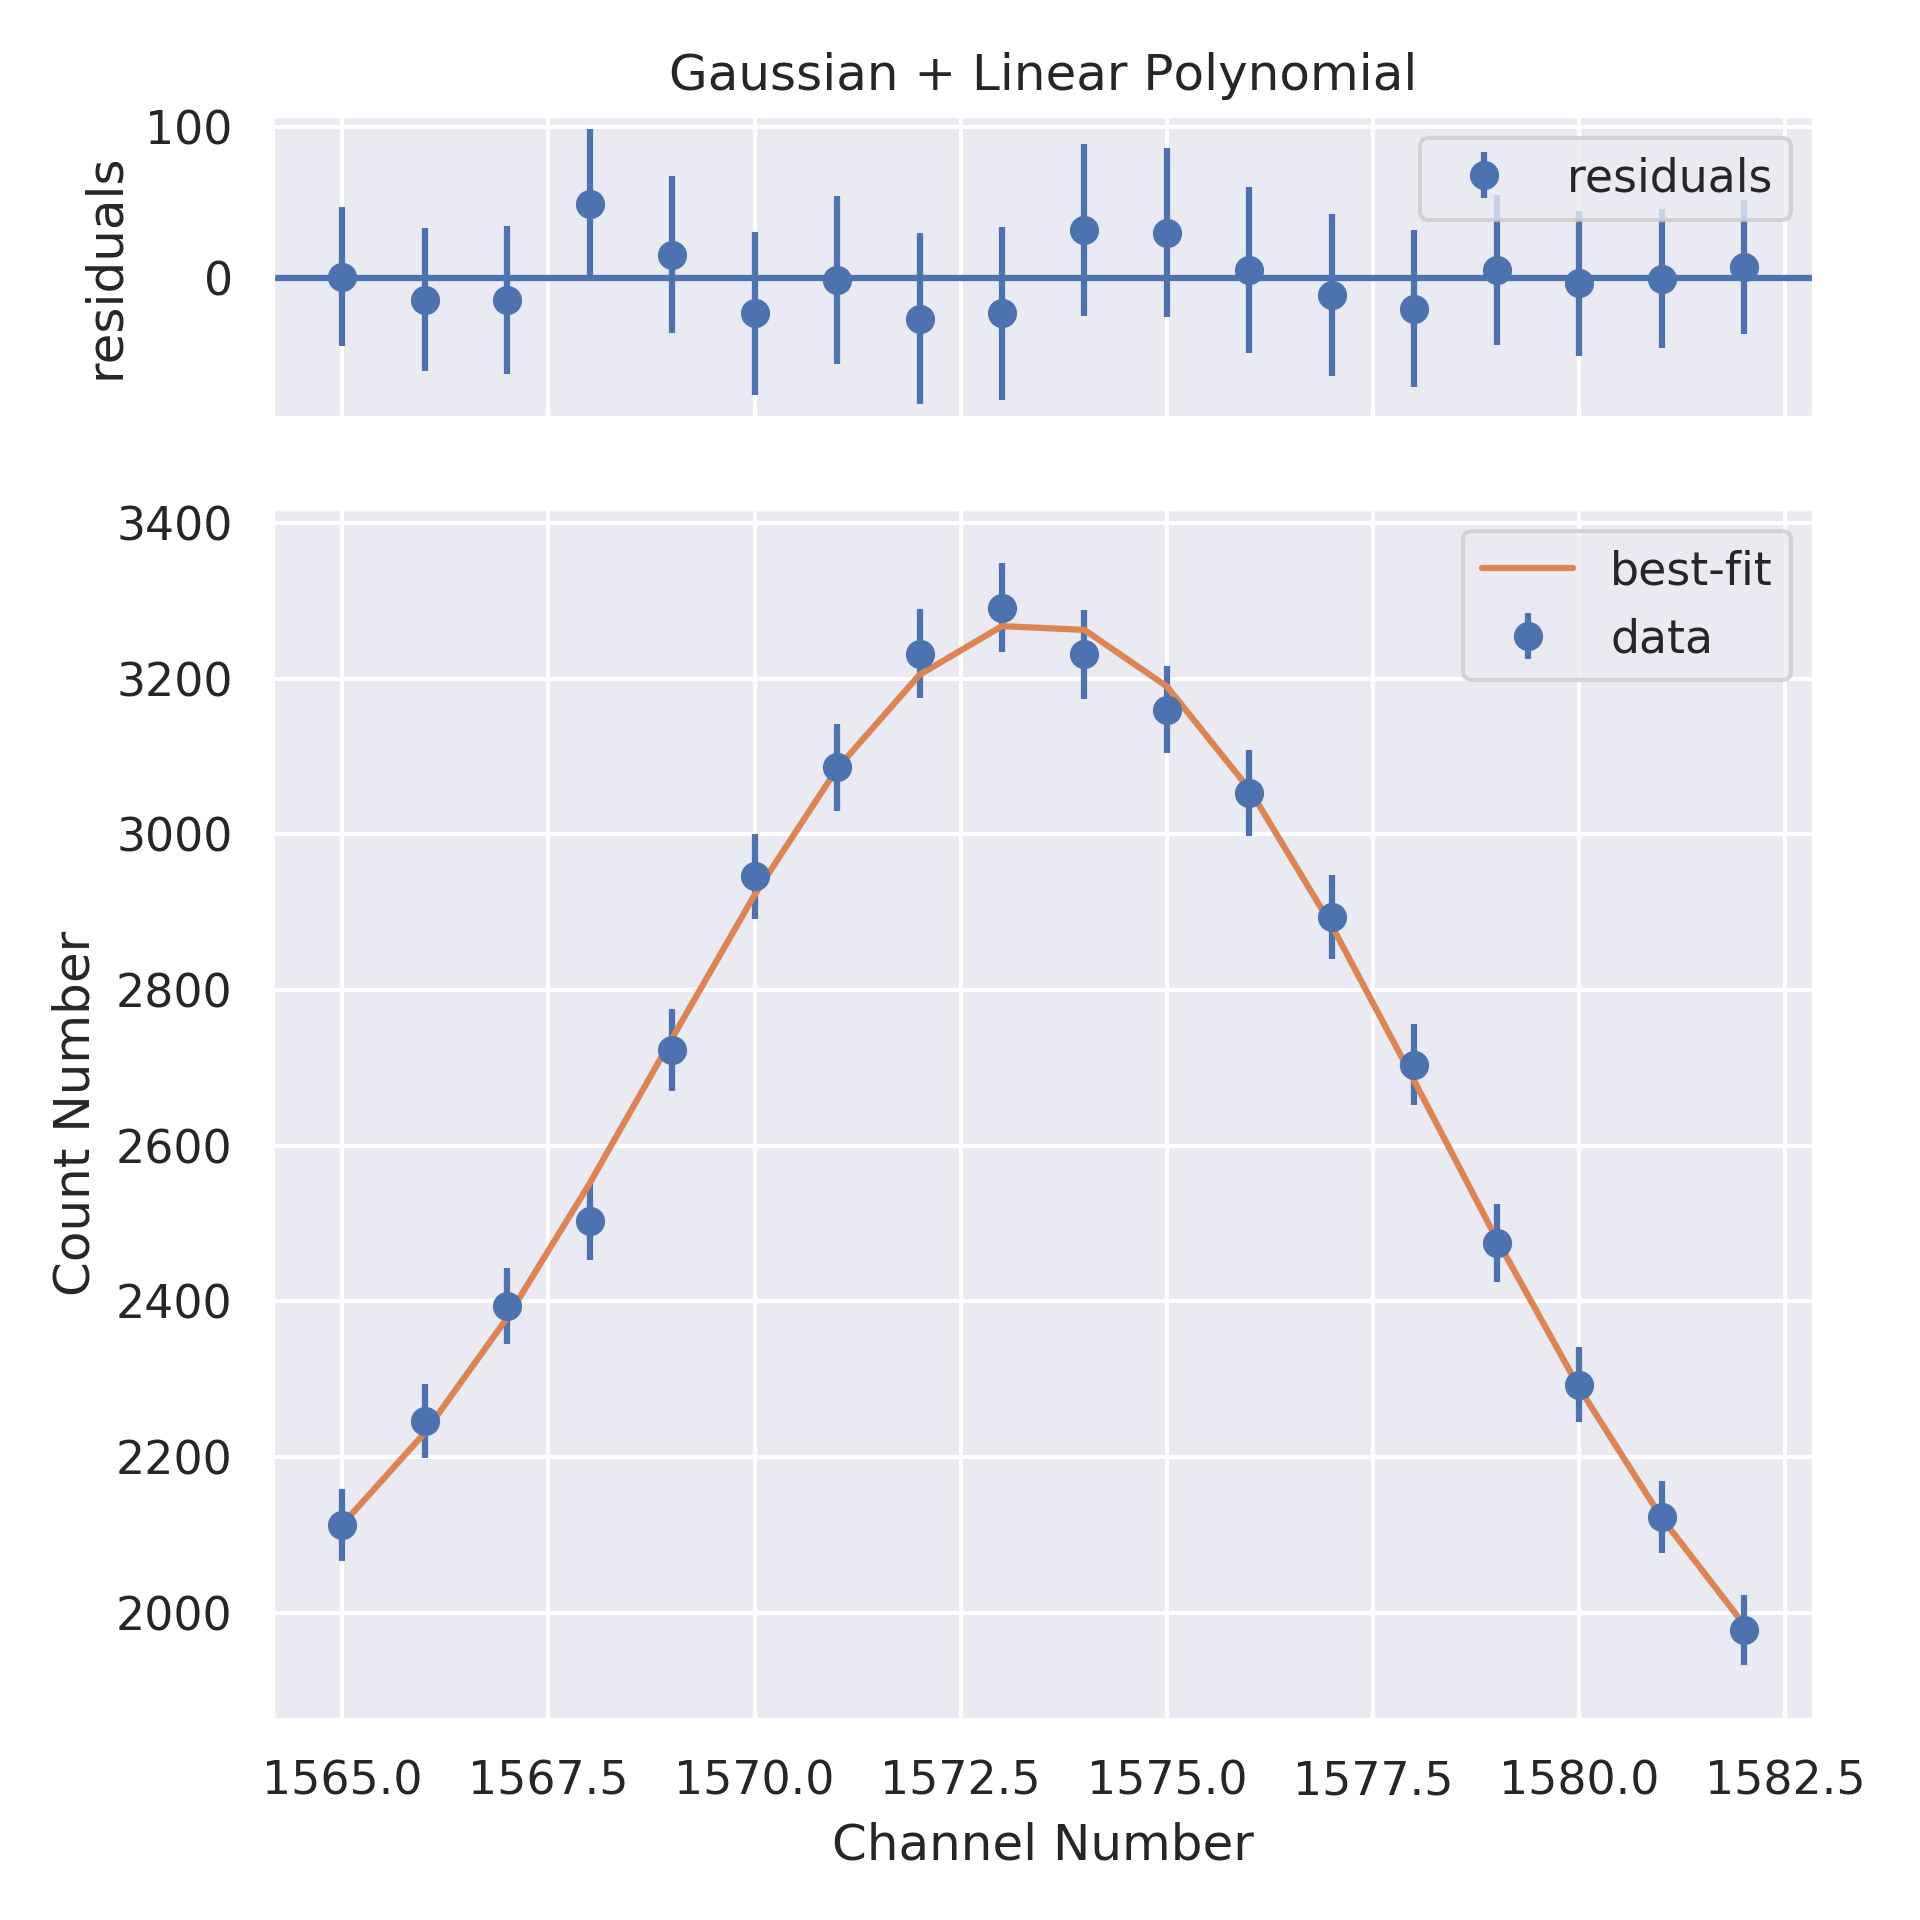
\includegraphics[width=\linewidth]{./Images/Barium133/Linear/Linear_3_Full.png}
    \caption{Full peak with fit. $\chi^2 = 2.65$, $\chi^2_\nu = 0.17$, \\ Prob = 99.99\%, $\mu = 1573.55$, $\sigma = 4.66$}
    %\label{fig:sub1}
  \end{subfigure}%
  \begin{subfigure}{.5\linewidth}
    \centering
    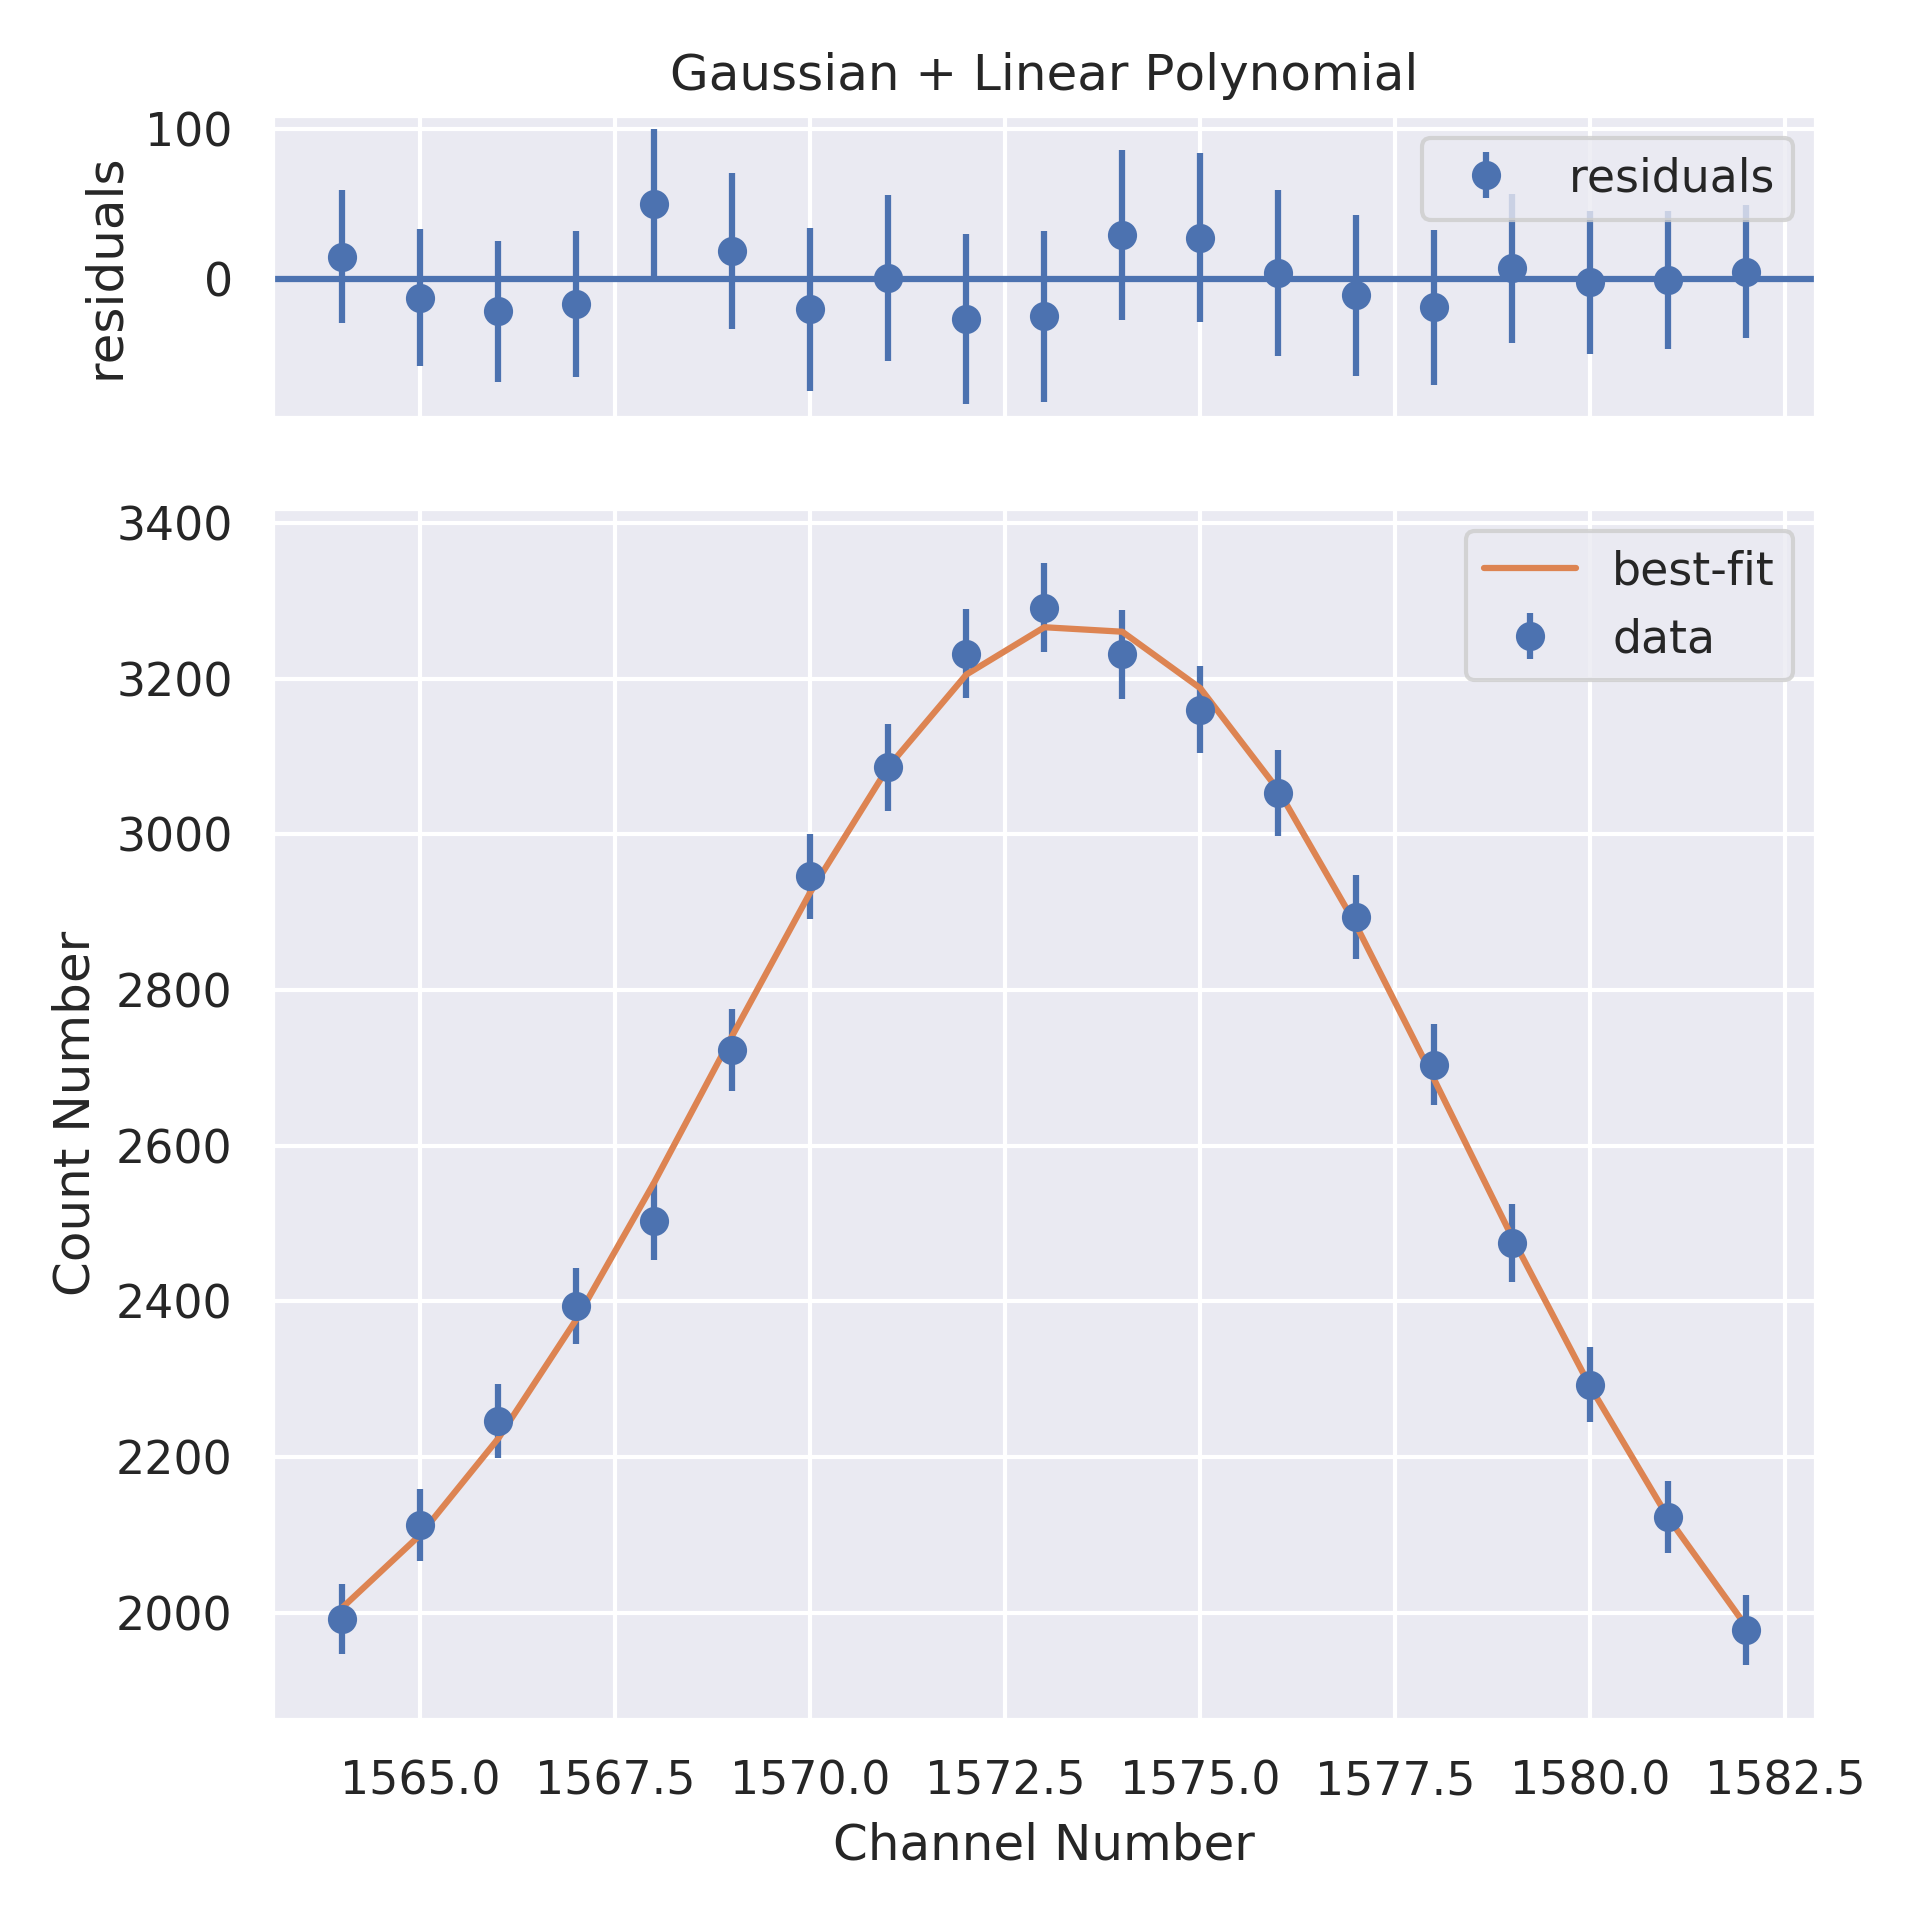
\includegraphics[width=\linewidth]{./Images/Barium133/Linear/Linear_3_Zoom.png}
    \caption{Zoomed in peak with fit. $\chi^2 = 2.93$, $\chi^2_\nu = 0.17$, \\ Prob = 99.99\%, $\mu = 1573.52$, $\sigma = 4.74$}
    %\label{fig:sub2}
  \end{subfigure}
  \caption{Fit of full \& zoomed in peak of \element{Ba}{133} 223 keV peak}
  %\label{fig:test}
\end{figure}
\begin{figure}[H]
  \centering
  \begin{subfigure}{.5\linewidth}
    \centering
    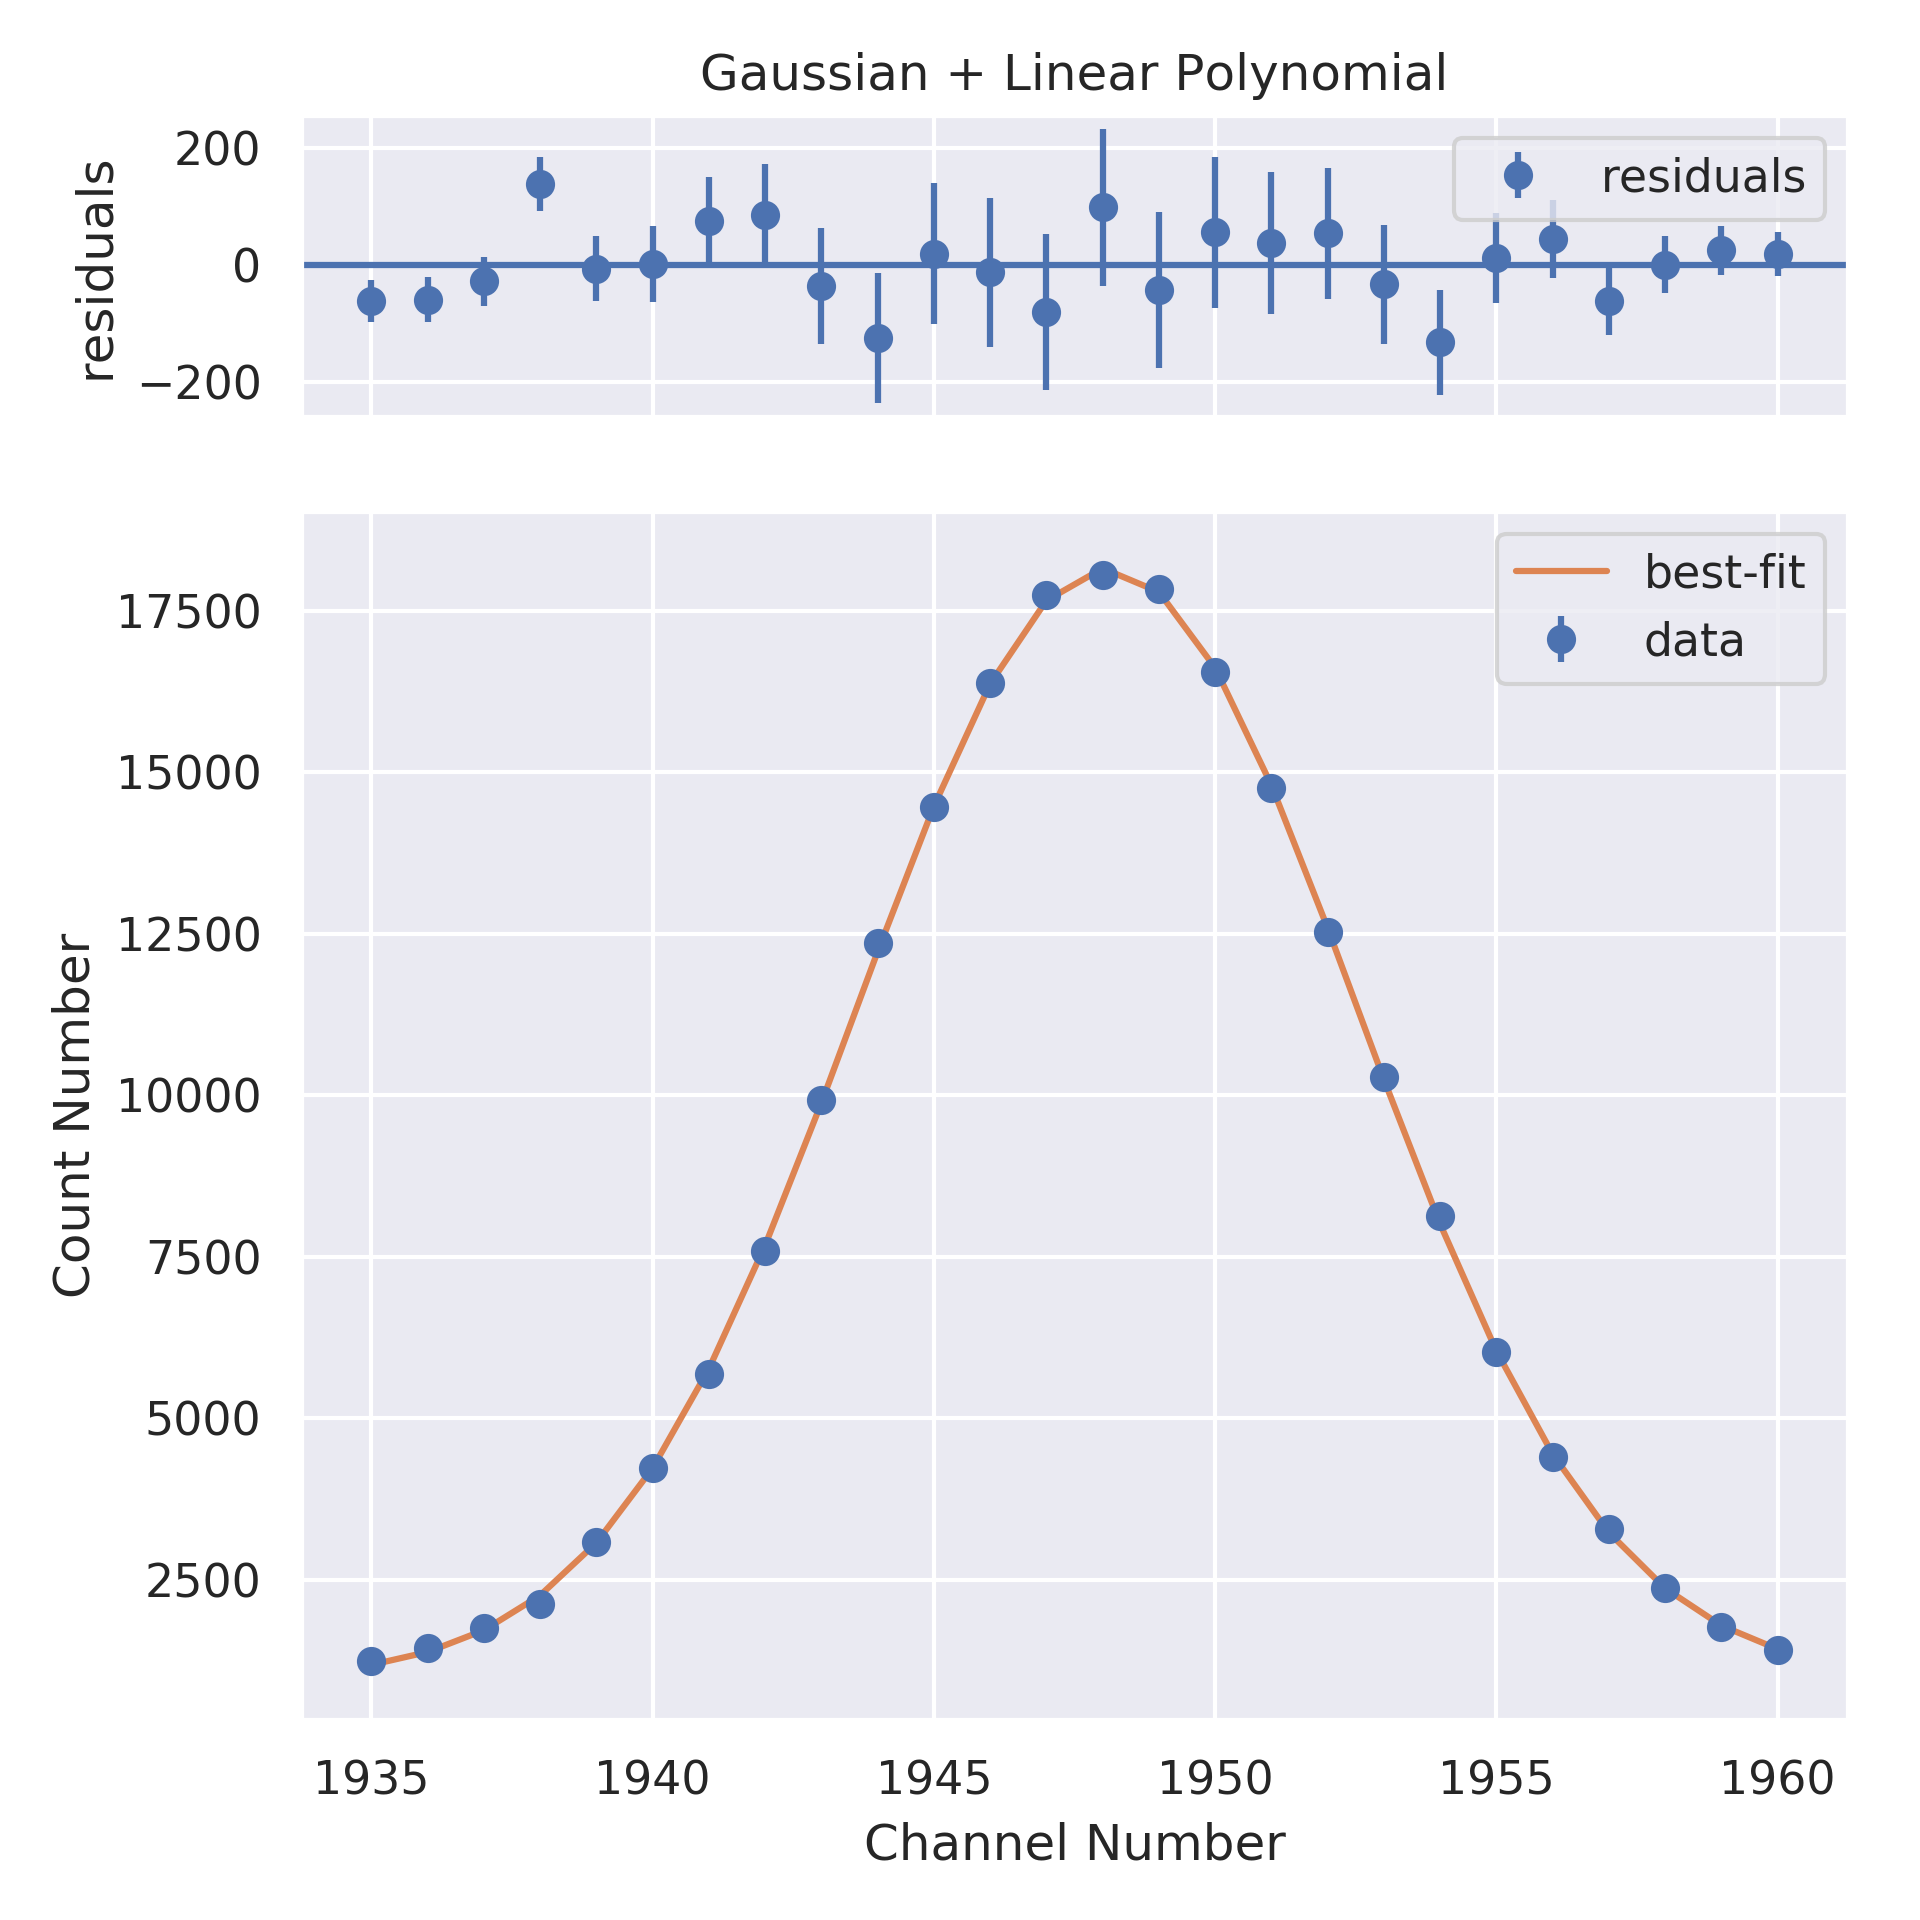
\includegraphics[width=\linewidth]{./Images/Barium133/Linear/Linear_4_Full.png}
    \caption{Full peak with fit. $\chi^2 = 24.39$, $\chi^2_\nu = 1.02$, \\ Prob = 43.93\%, $\mu = 1948.08$, $\sigma = 4.43$}
    %\label{fig:sub1}
  \end{subfigure}%
  \begin{subfigure}{.5\linewidth}
    \centering
    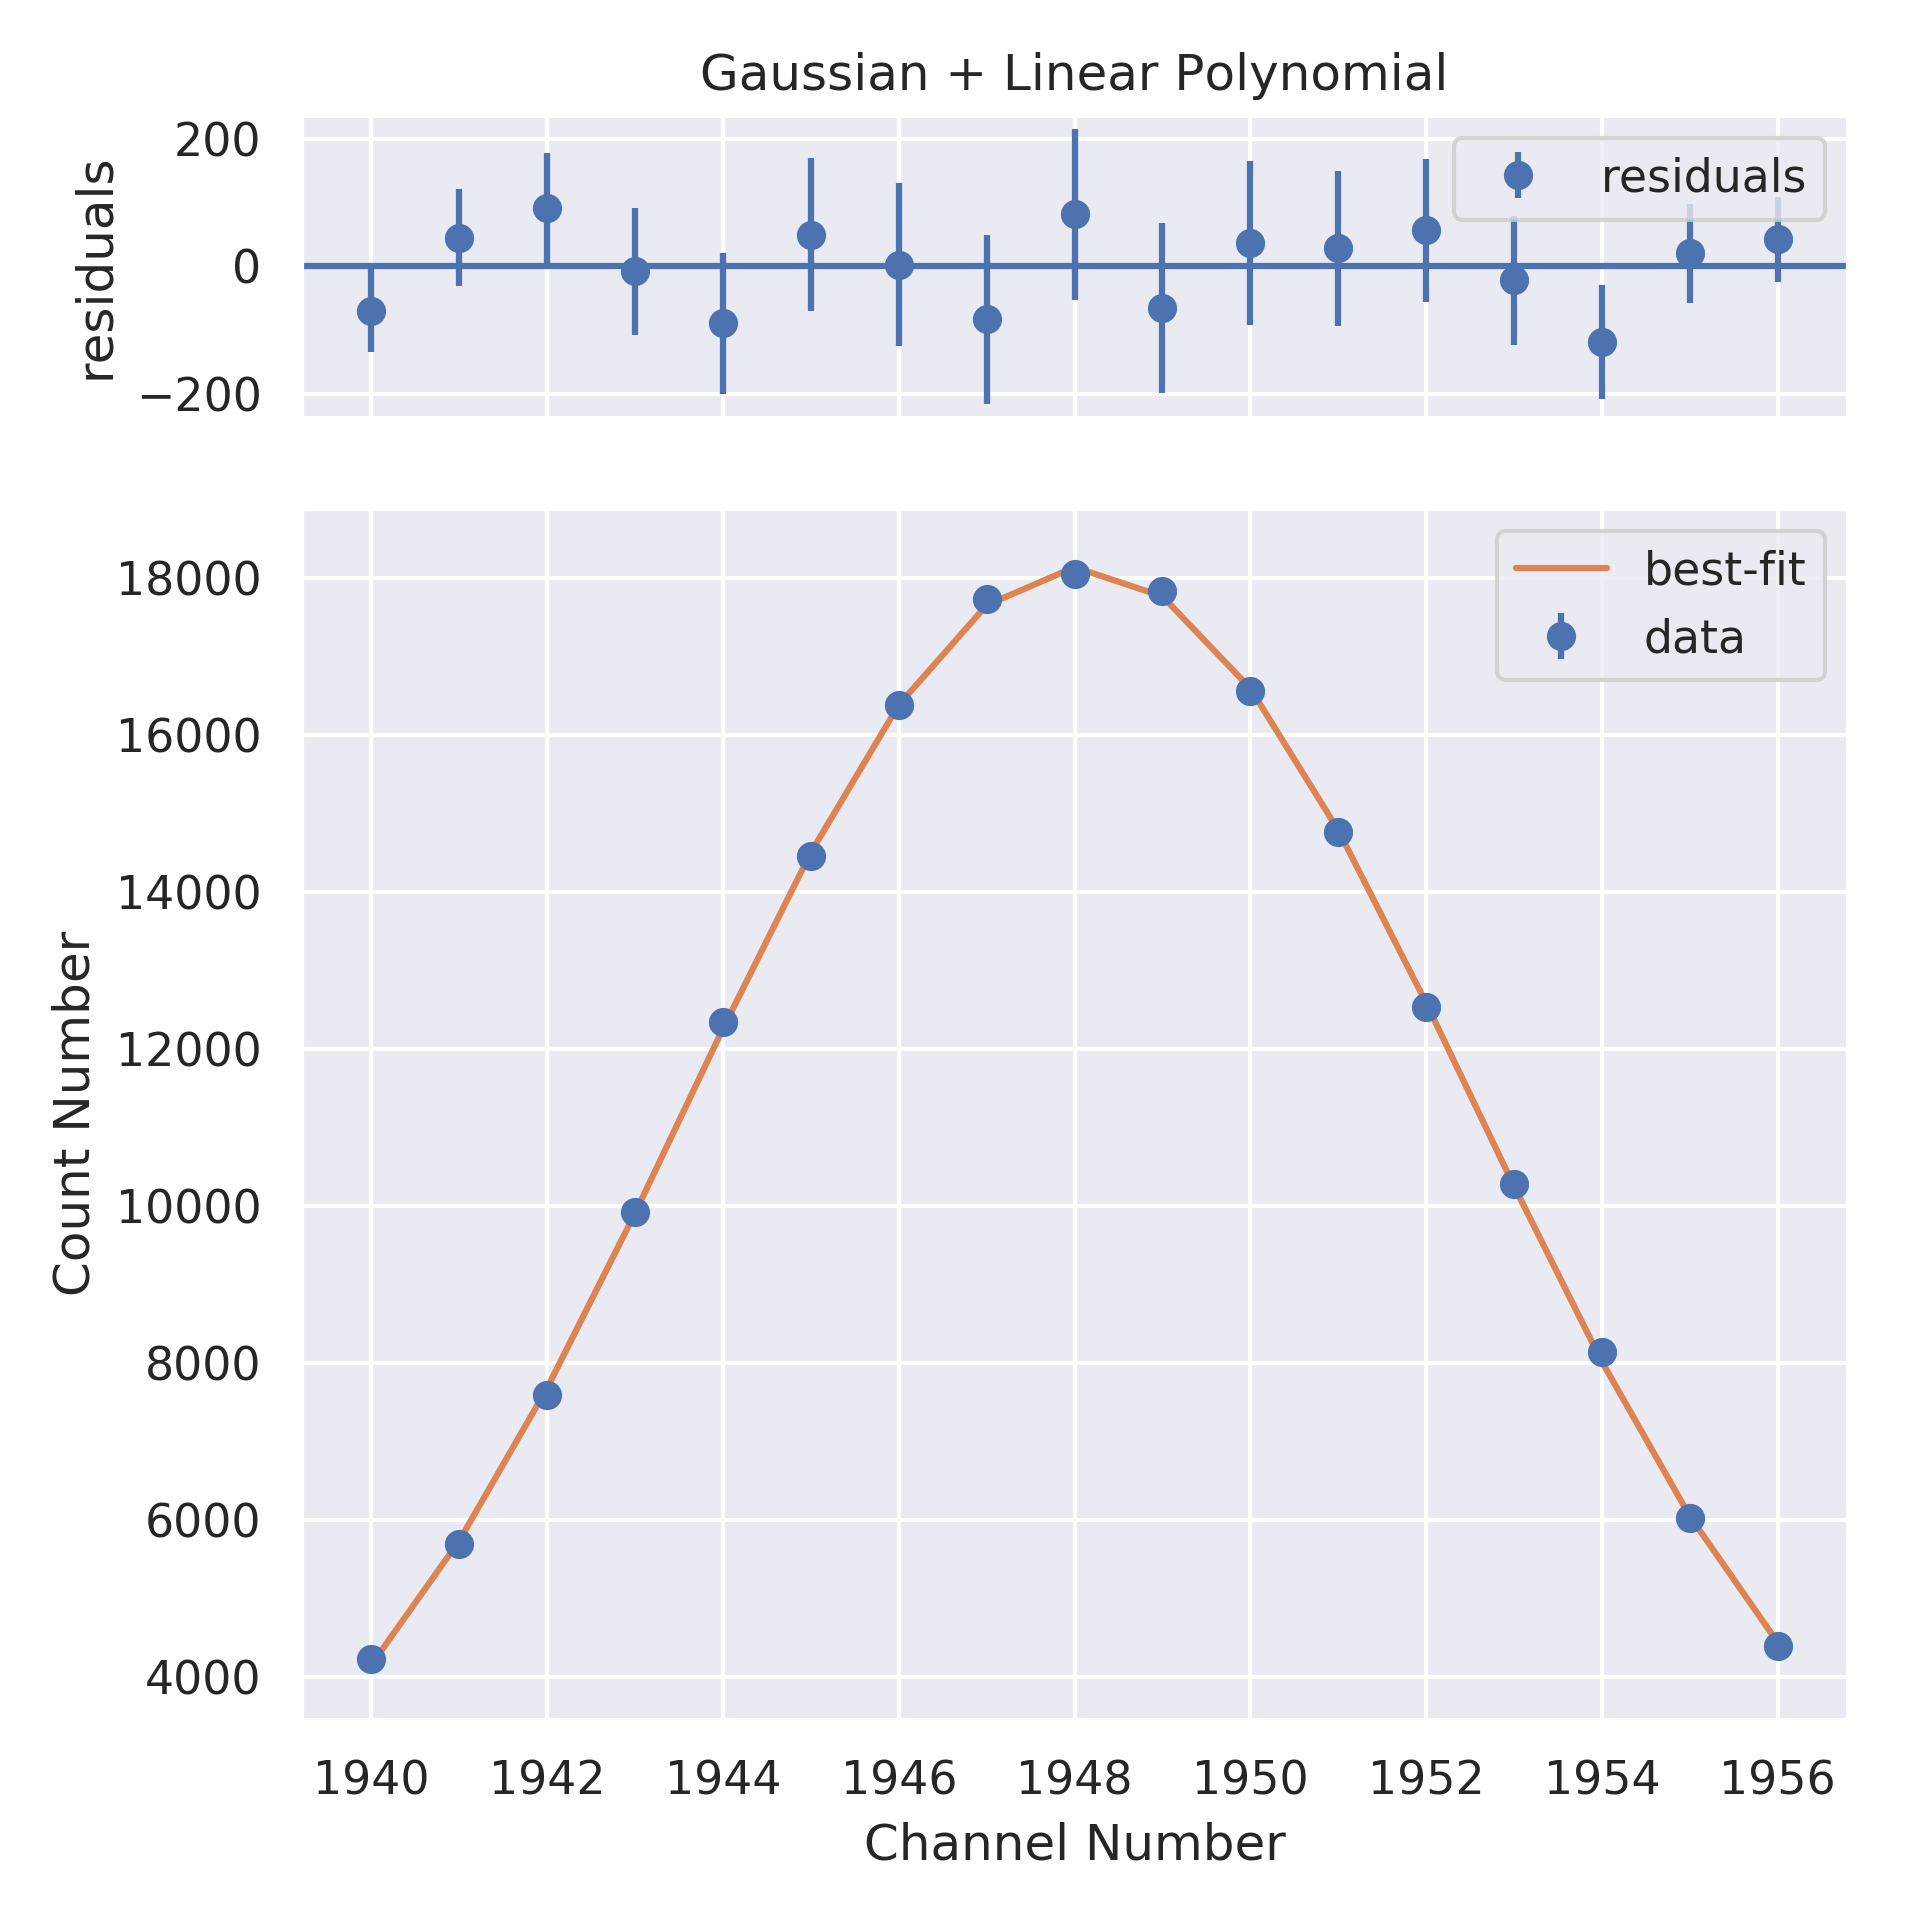
\includegraphics[width=\linewidth]{./Images/Barium133/Linear/Linear_4_Zoom.png}
    \caption{Zoomed in peak with fit. $\chi^2 = 7.08$, $\chi^2_\nu = 0.47$, \\ Prob = 95.54\%, $\mu = 1948.06$, $\sigma = 4.47$}
    %\label{fig:sub2}
  \end{subfigure}
  \caption{Fit of full \& zoomed in peak of \element{Ba}{133} 276 keV peak}
  %\label{fig:test}
\end{figure}
\begin{figure}[H]
  \centering
  \begin{subfigure}{.5\linewidth}
    \centering
    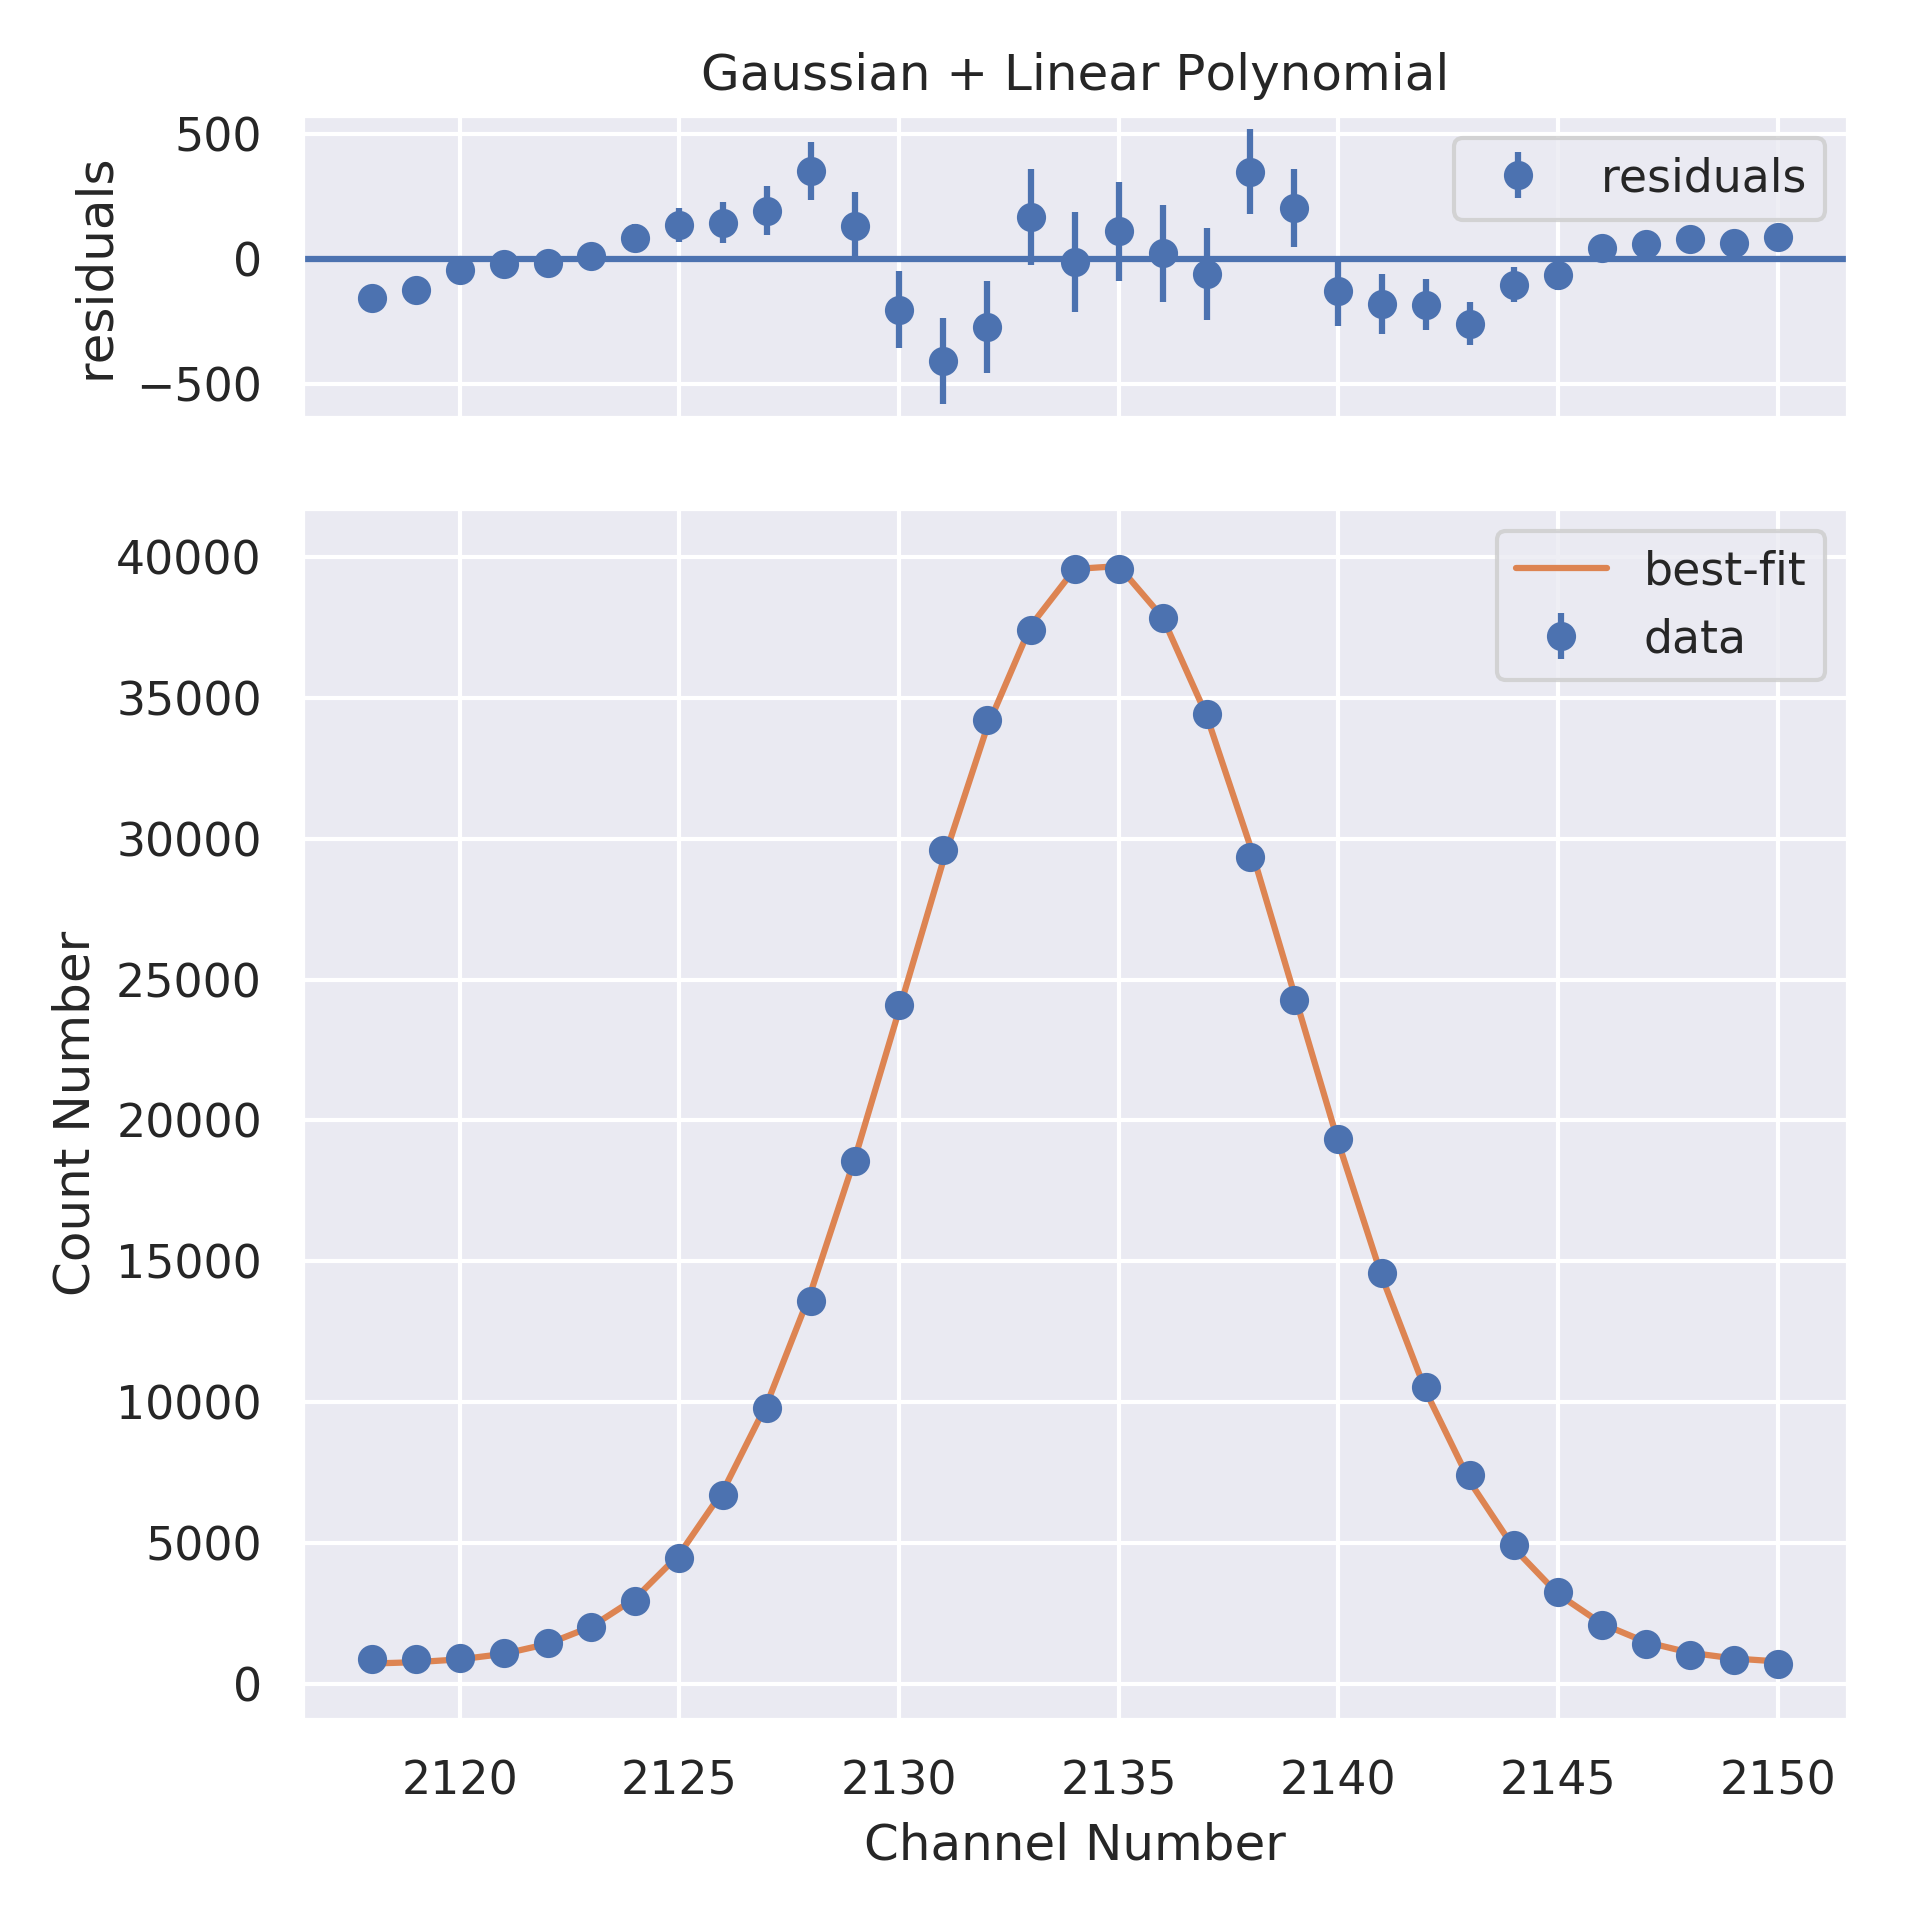
\includegraphics[width=\linewidth]{./Images/Barium133/Linear/Linear_5_Full.png}
    \caption{Full peak with fit. $\chi^2 = 131.45$, $\chi^2_\nu = 4.24$, \\ Prob = 0\%, $\mu = 2134.55$, $\sigma = 4.45$}
    %\label{fig:sub1}
  \end{subfigure}%
  \begin{subfigure}{.5\linewidth}
    \centering
    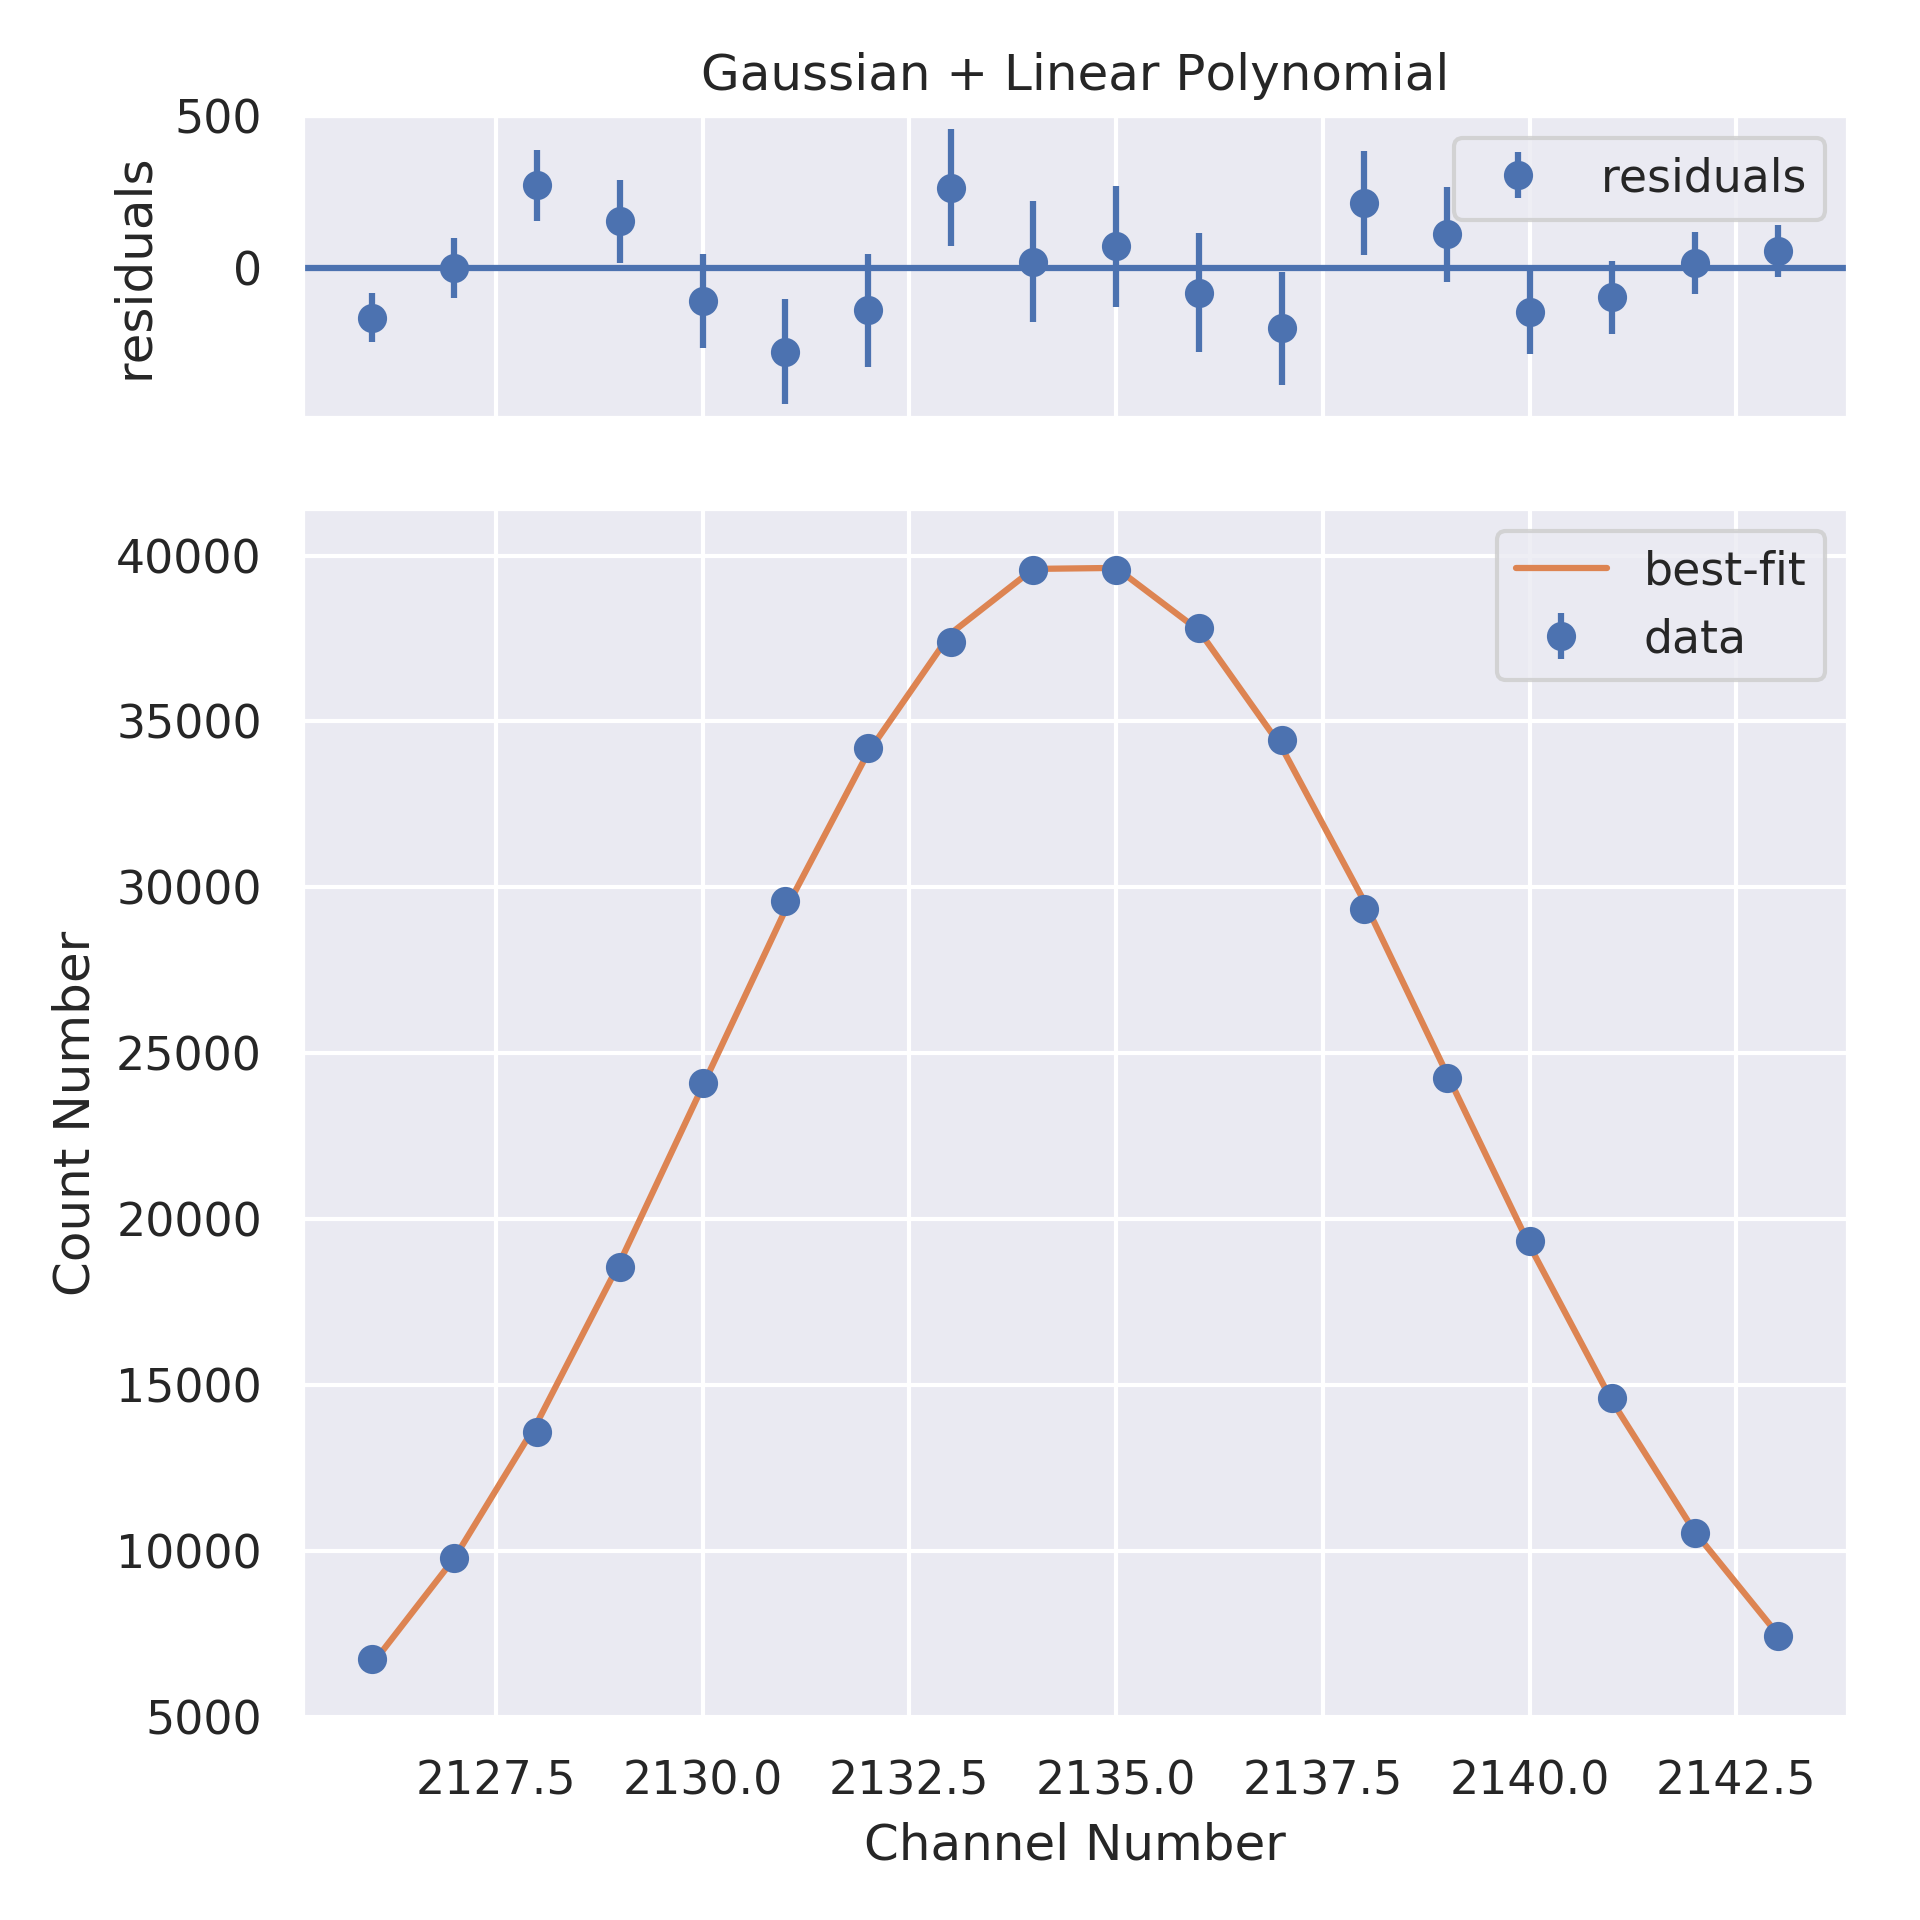
\includegraphics[width=\linewidth]{./Images/Barium133/Linear/Linear_5_Zoom.png}
    \caption{Zoomed in peak with fit. $\chi^2 = 21.84$, $\chi^2_\nu = 1.36$, \\ Prob = 14.85\%, $\mu = 2134.49$, $\sigma = 4.45$}
    %\label{fig:sub2}
  \end{subfigure}
  \caption{Fit of full \& zoomed in peak of \element{Ba}{133} 303 keV peak}
  %\label{fig:test}
\end{figure}
\begin{figure}[H]
  \centering
  \begin{subfigure}{.5\linewidth}
    \centering
    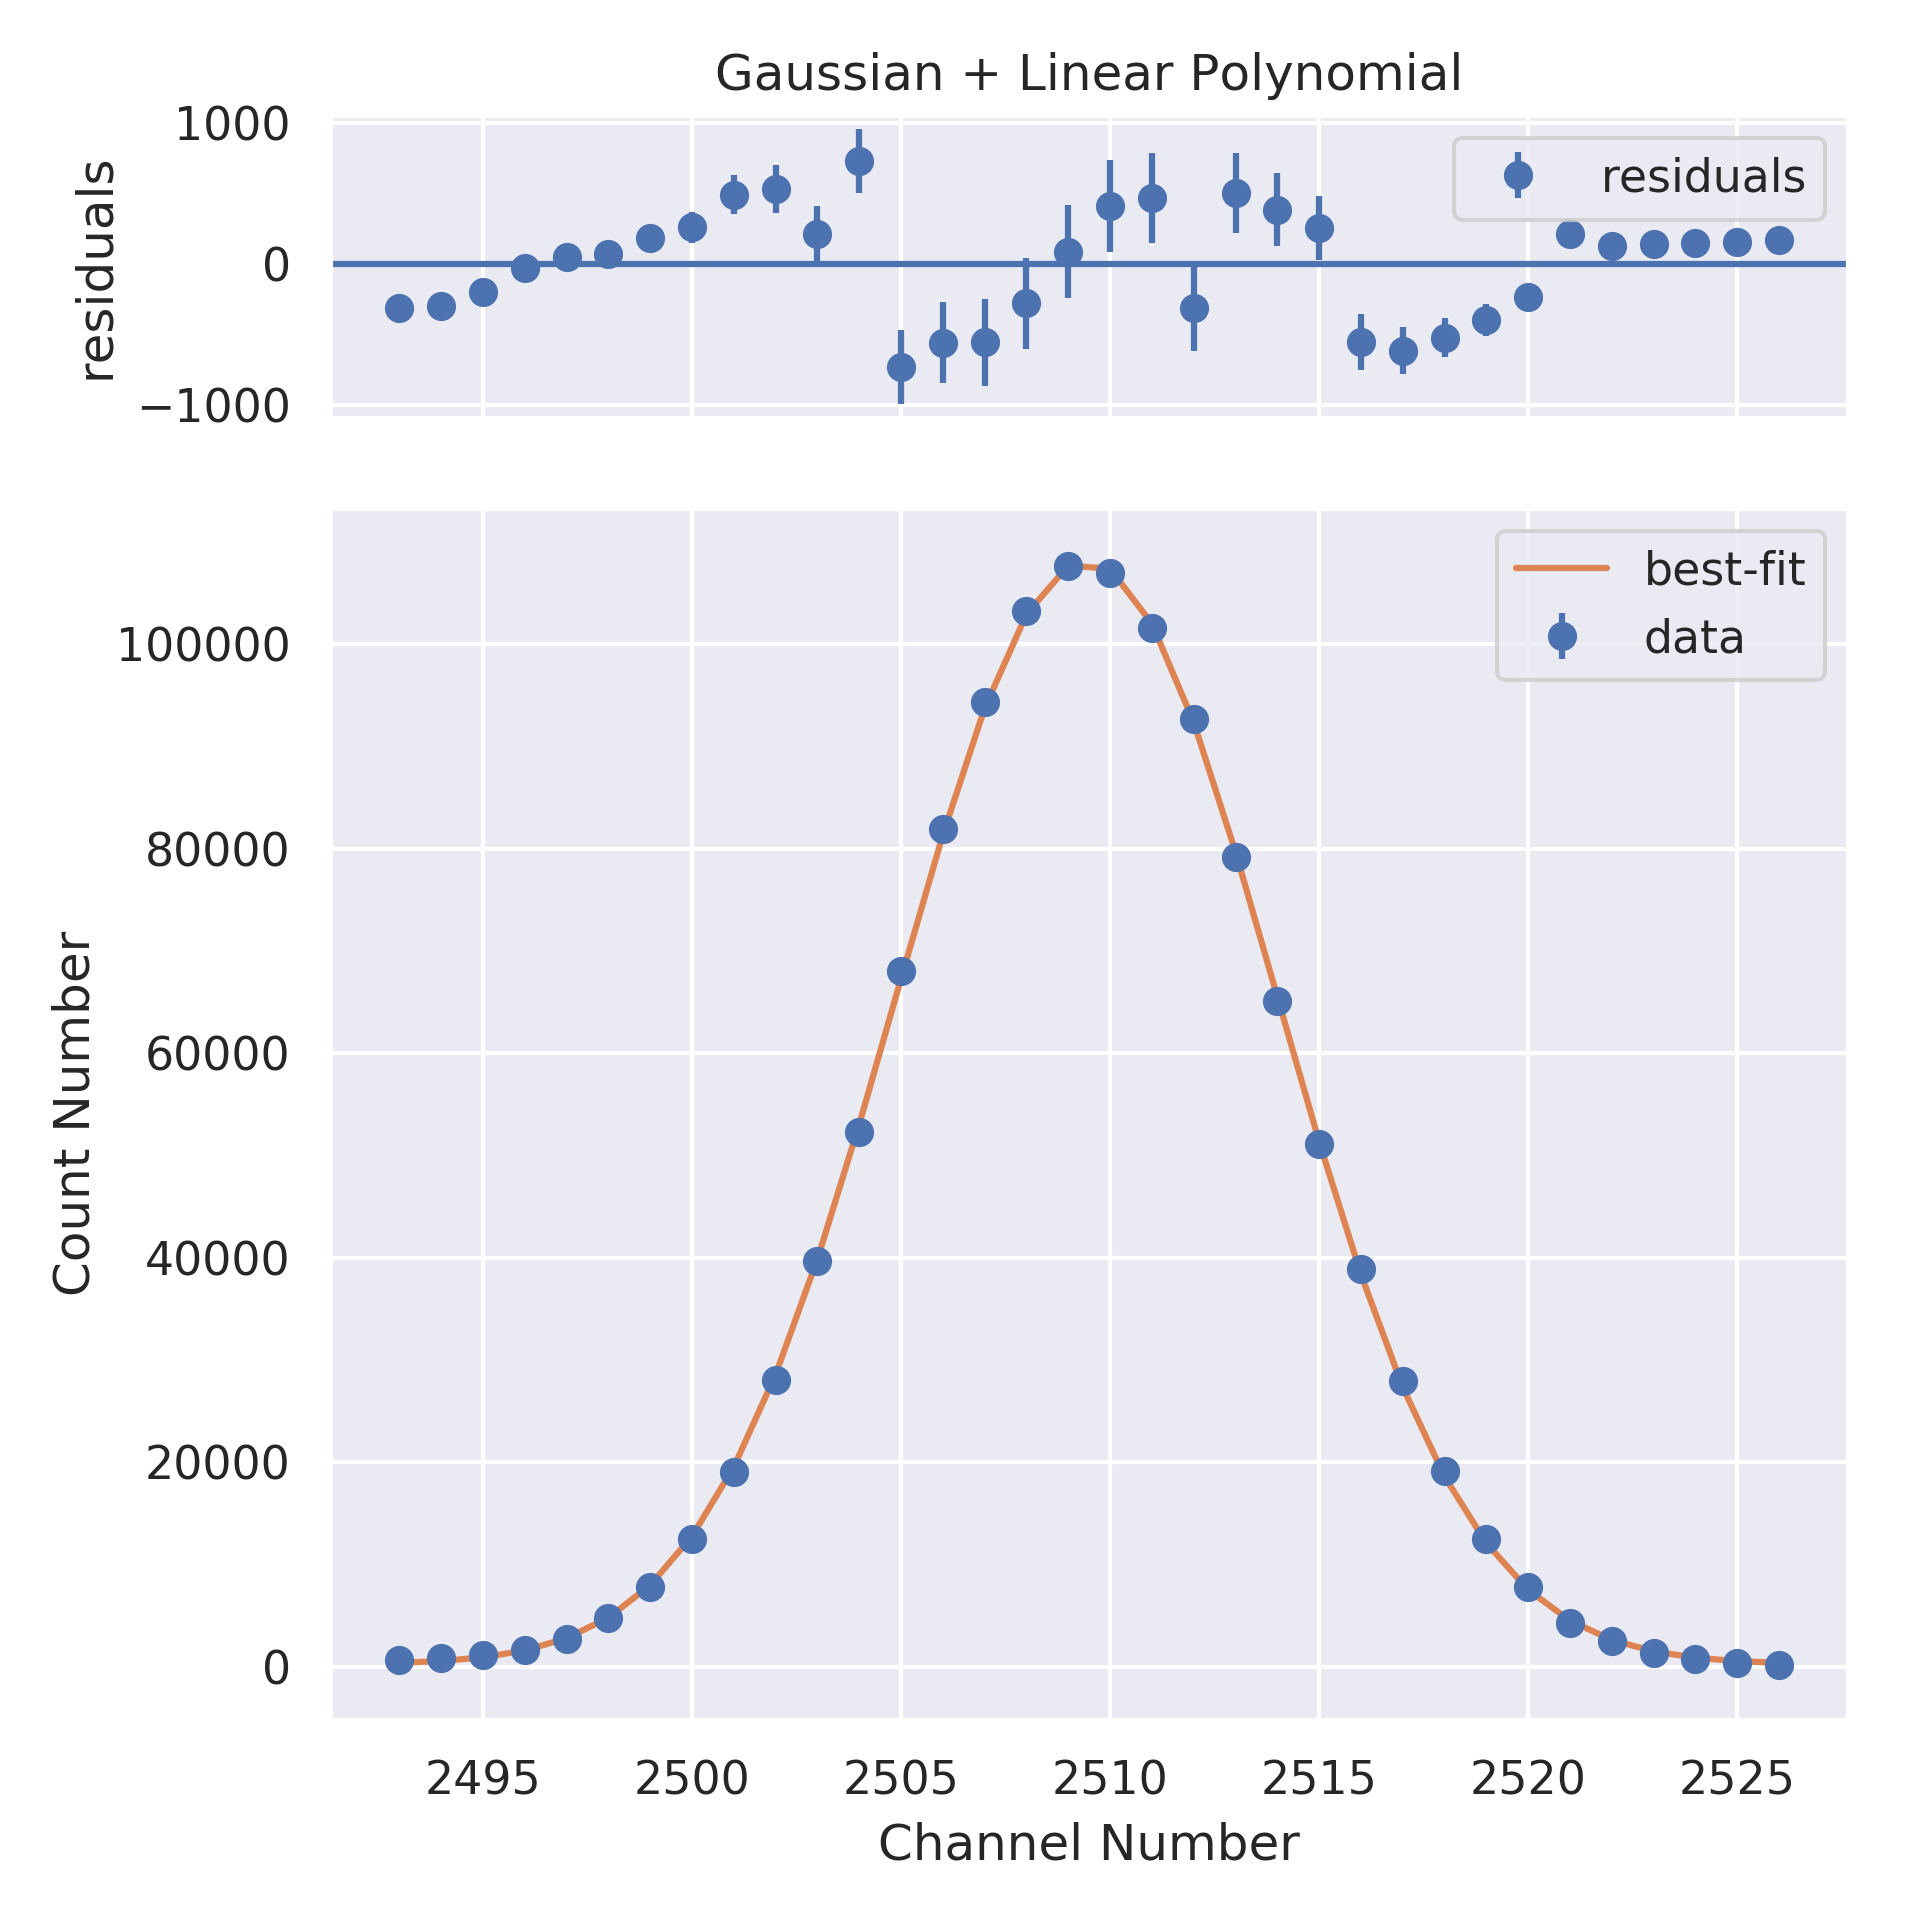
\includegraphics[width=\linewidth]{./Images/Barium133/Linear/Linear_6_Full.png}
    \caption{Full peak with fit. $\chi^2 = 658.02$, $\chi^2_\nu = 20.56$, \\ Prob = 0\%, $\mu = 2509.44$, $\sigma = 4.55$}
    %\label{fig:sub1}
  \end{subfigure}%
  \begin{subfigure}{.5\linewidth}
    \centering
    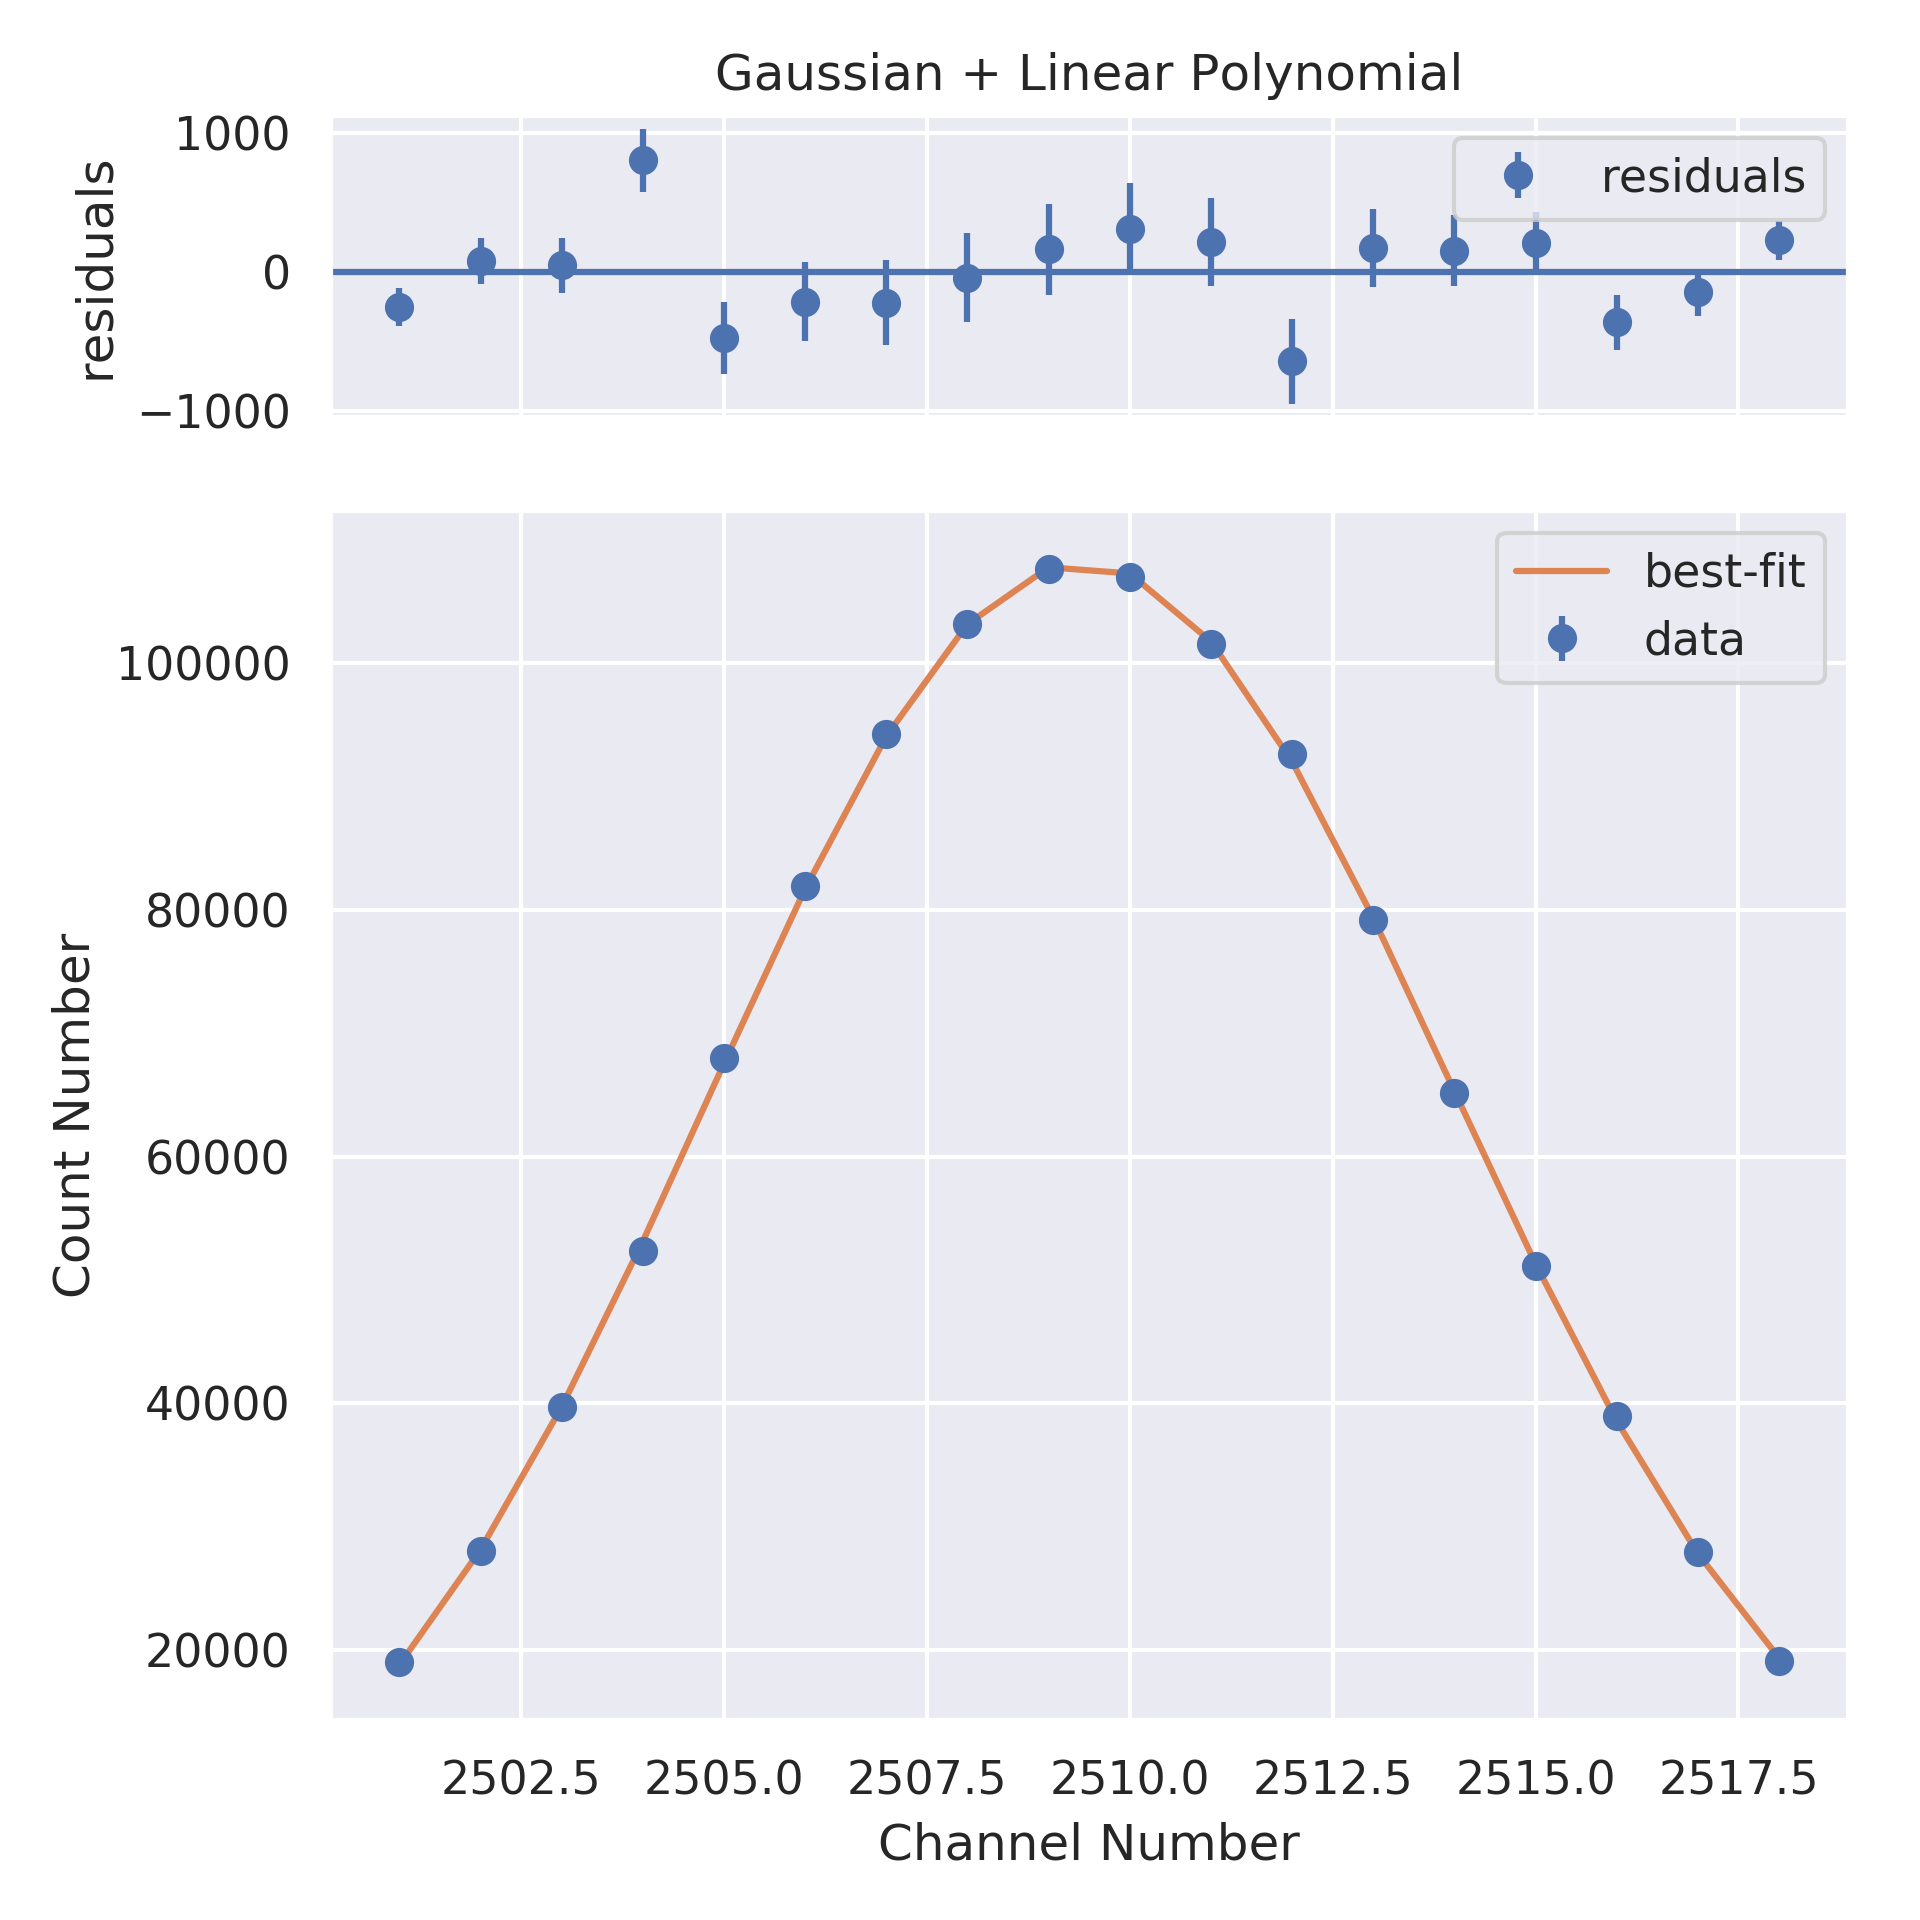
\includegraphics[width=\linewidth]{./Images/Barium133/Linear/Linear_6_Zoom.png}
    \caption{Zoomed in peak with fit. $\chi^2 = 34.92$, $\chi^2_\nu = 2.18$, \\ Prob = 0.41\%, $\mu = 2509.38$, $\sigma = 4.55$}
    %\label{fig:sub2}
  \end{subfigure}
  \caption{Fit of full \& zoomed in peak of \element{Ba}{133} 356 keV peak}
  %\label{fig:test}
\end{figure}
\begin{figure}[H]
  \centering
  \begin{subfigure}{.5\linewidth}
    \centering
    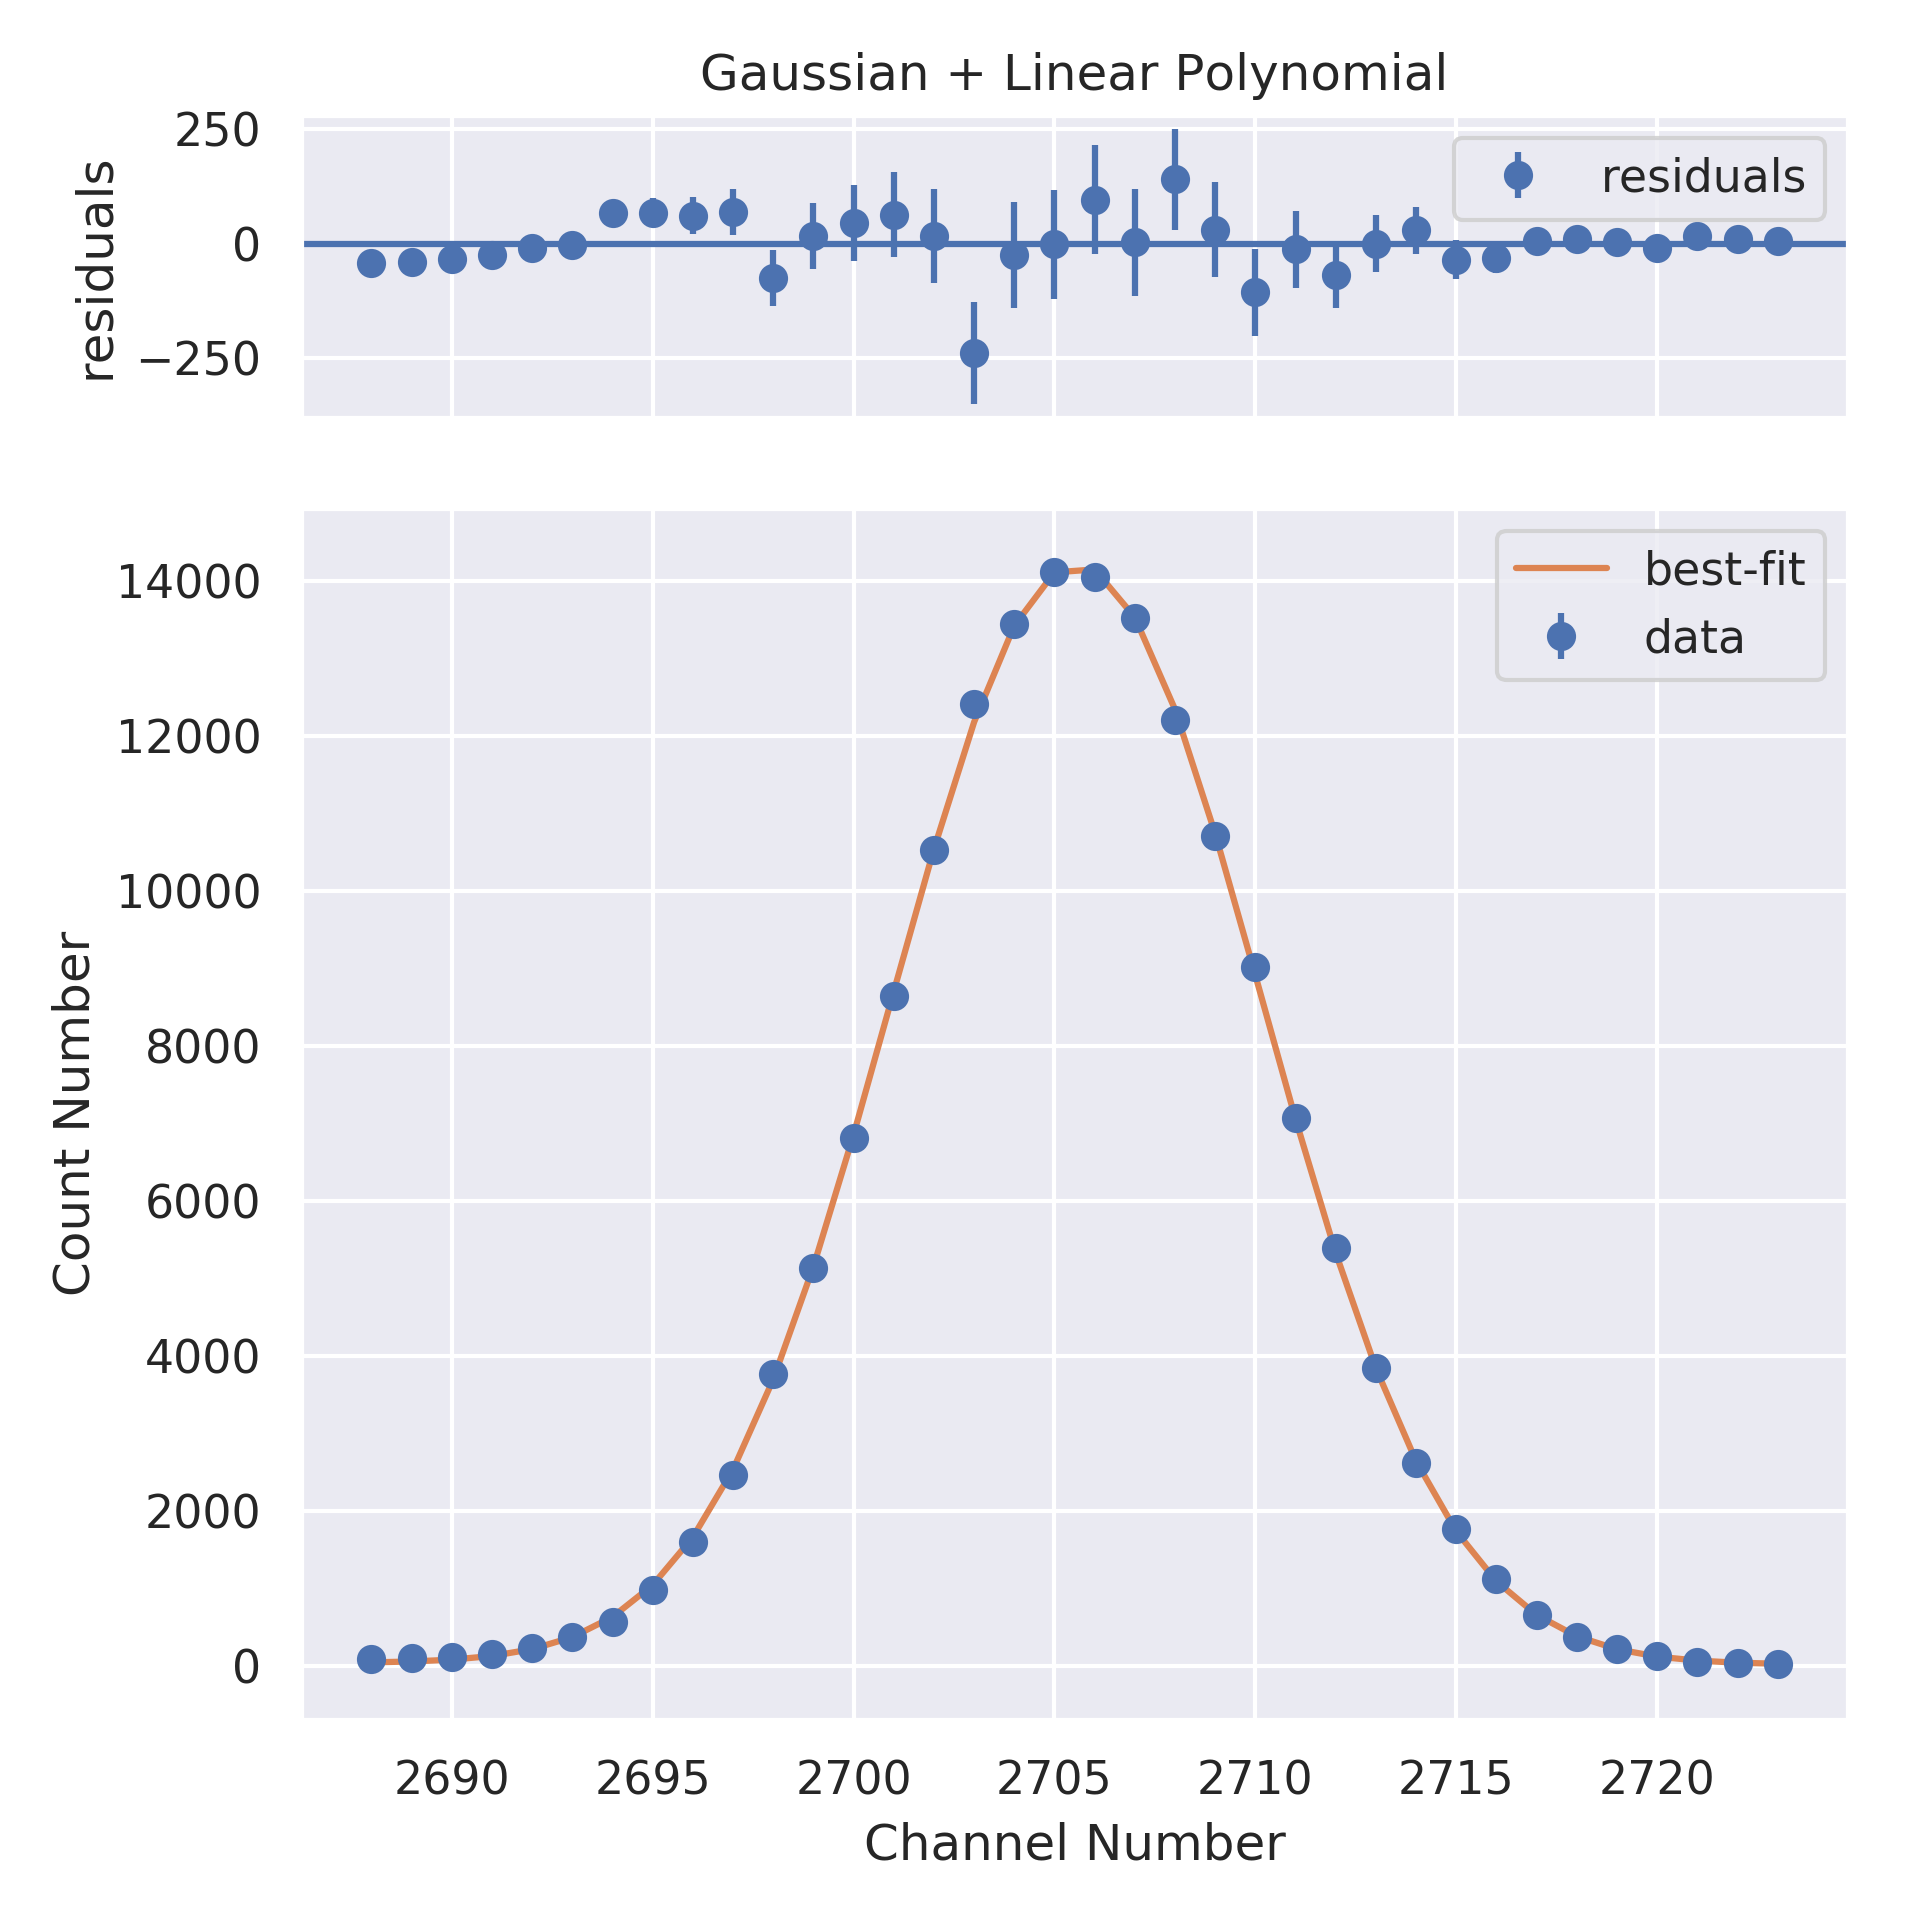
\includegraphics[width=\linewidth]{./Images/Barium133/Linear/Linear_7_Full.png}
    \caption{Full peak with fit. $\chi^2 = 85.03$, $\chi^2_\nu = 2.50$, \\ Prob = 0\%, $\mu = 2705.06$, $\sigma = 4.59$}
    %\label{fig:sub1}
  \end{subfigure}%
  \begin{subfigure}{.5\linewidth}
    \centering
    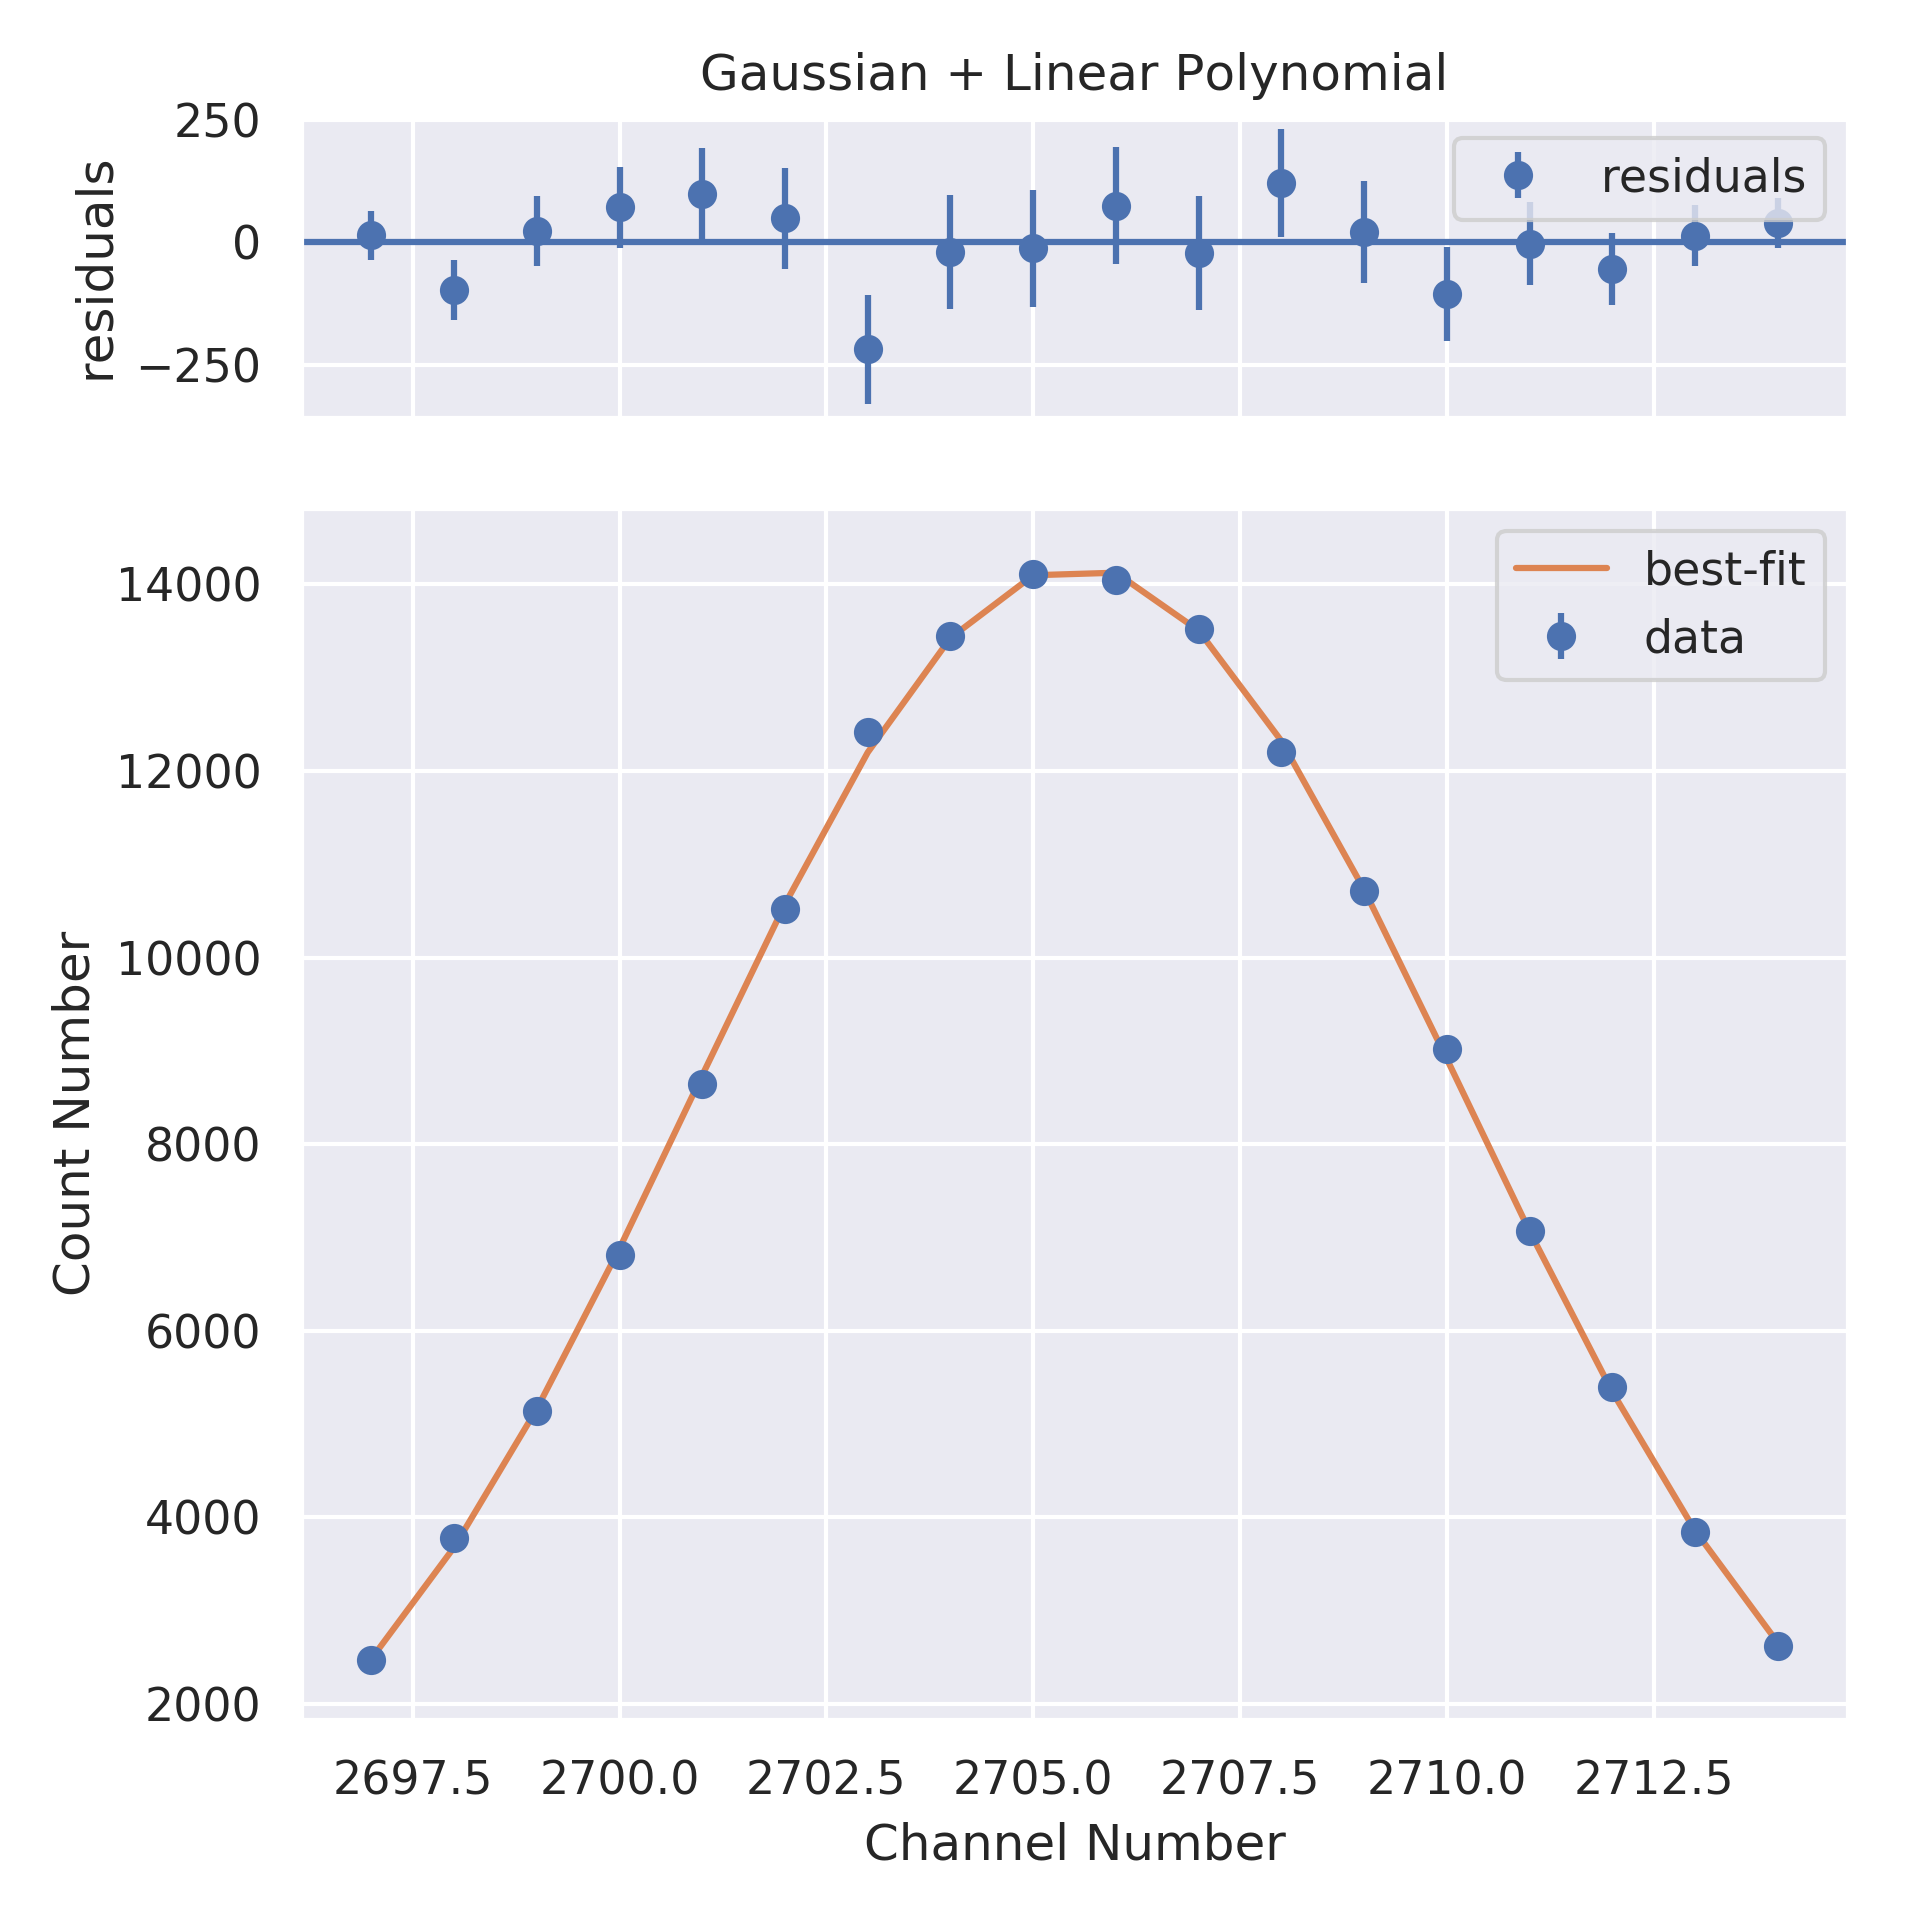
\includegraphics[width=\linewidth]{./Images/Barium133/Linear/Linear_7_Zoom.png}
    \caption{Zoomed in peak with fit. $\chi^2 = 12.68$, $\chi^2_\nu = 0.79$, \\ Prob = 69.69\%, $\mu = 2705.53$, $\sigma = 4.63$}
    %\label{fig:sub2}
  \end{subfigure}
  \caption{Fit of full \& zoomed in peak of \element{Ba}{133} 384 keV peak}
  %\label{fig:test}
\end{figure}
\clearpage
\subsubsection{Gaussian + Quadratic Fit}
\begin{figure}[H]
  \centering
  \begin{subfigure}{.5\linewidth}
    \centering
    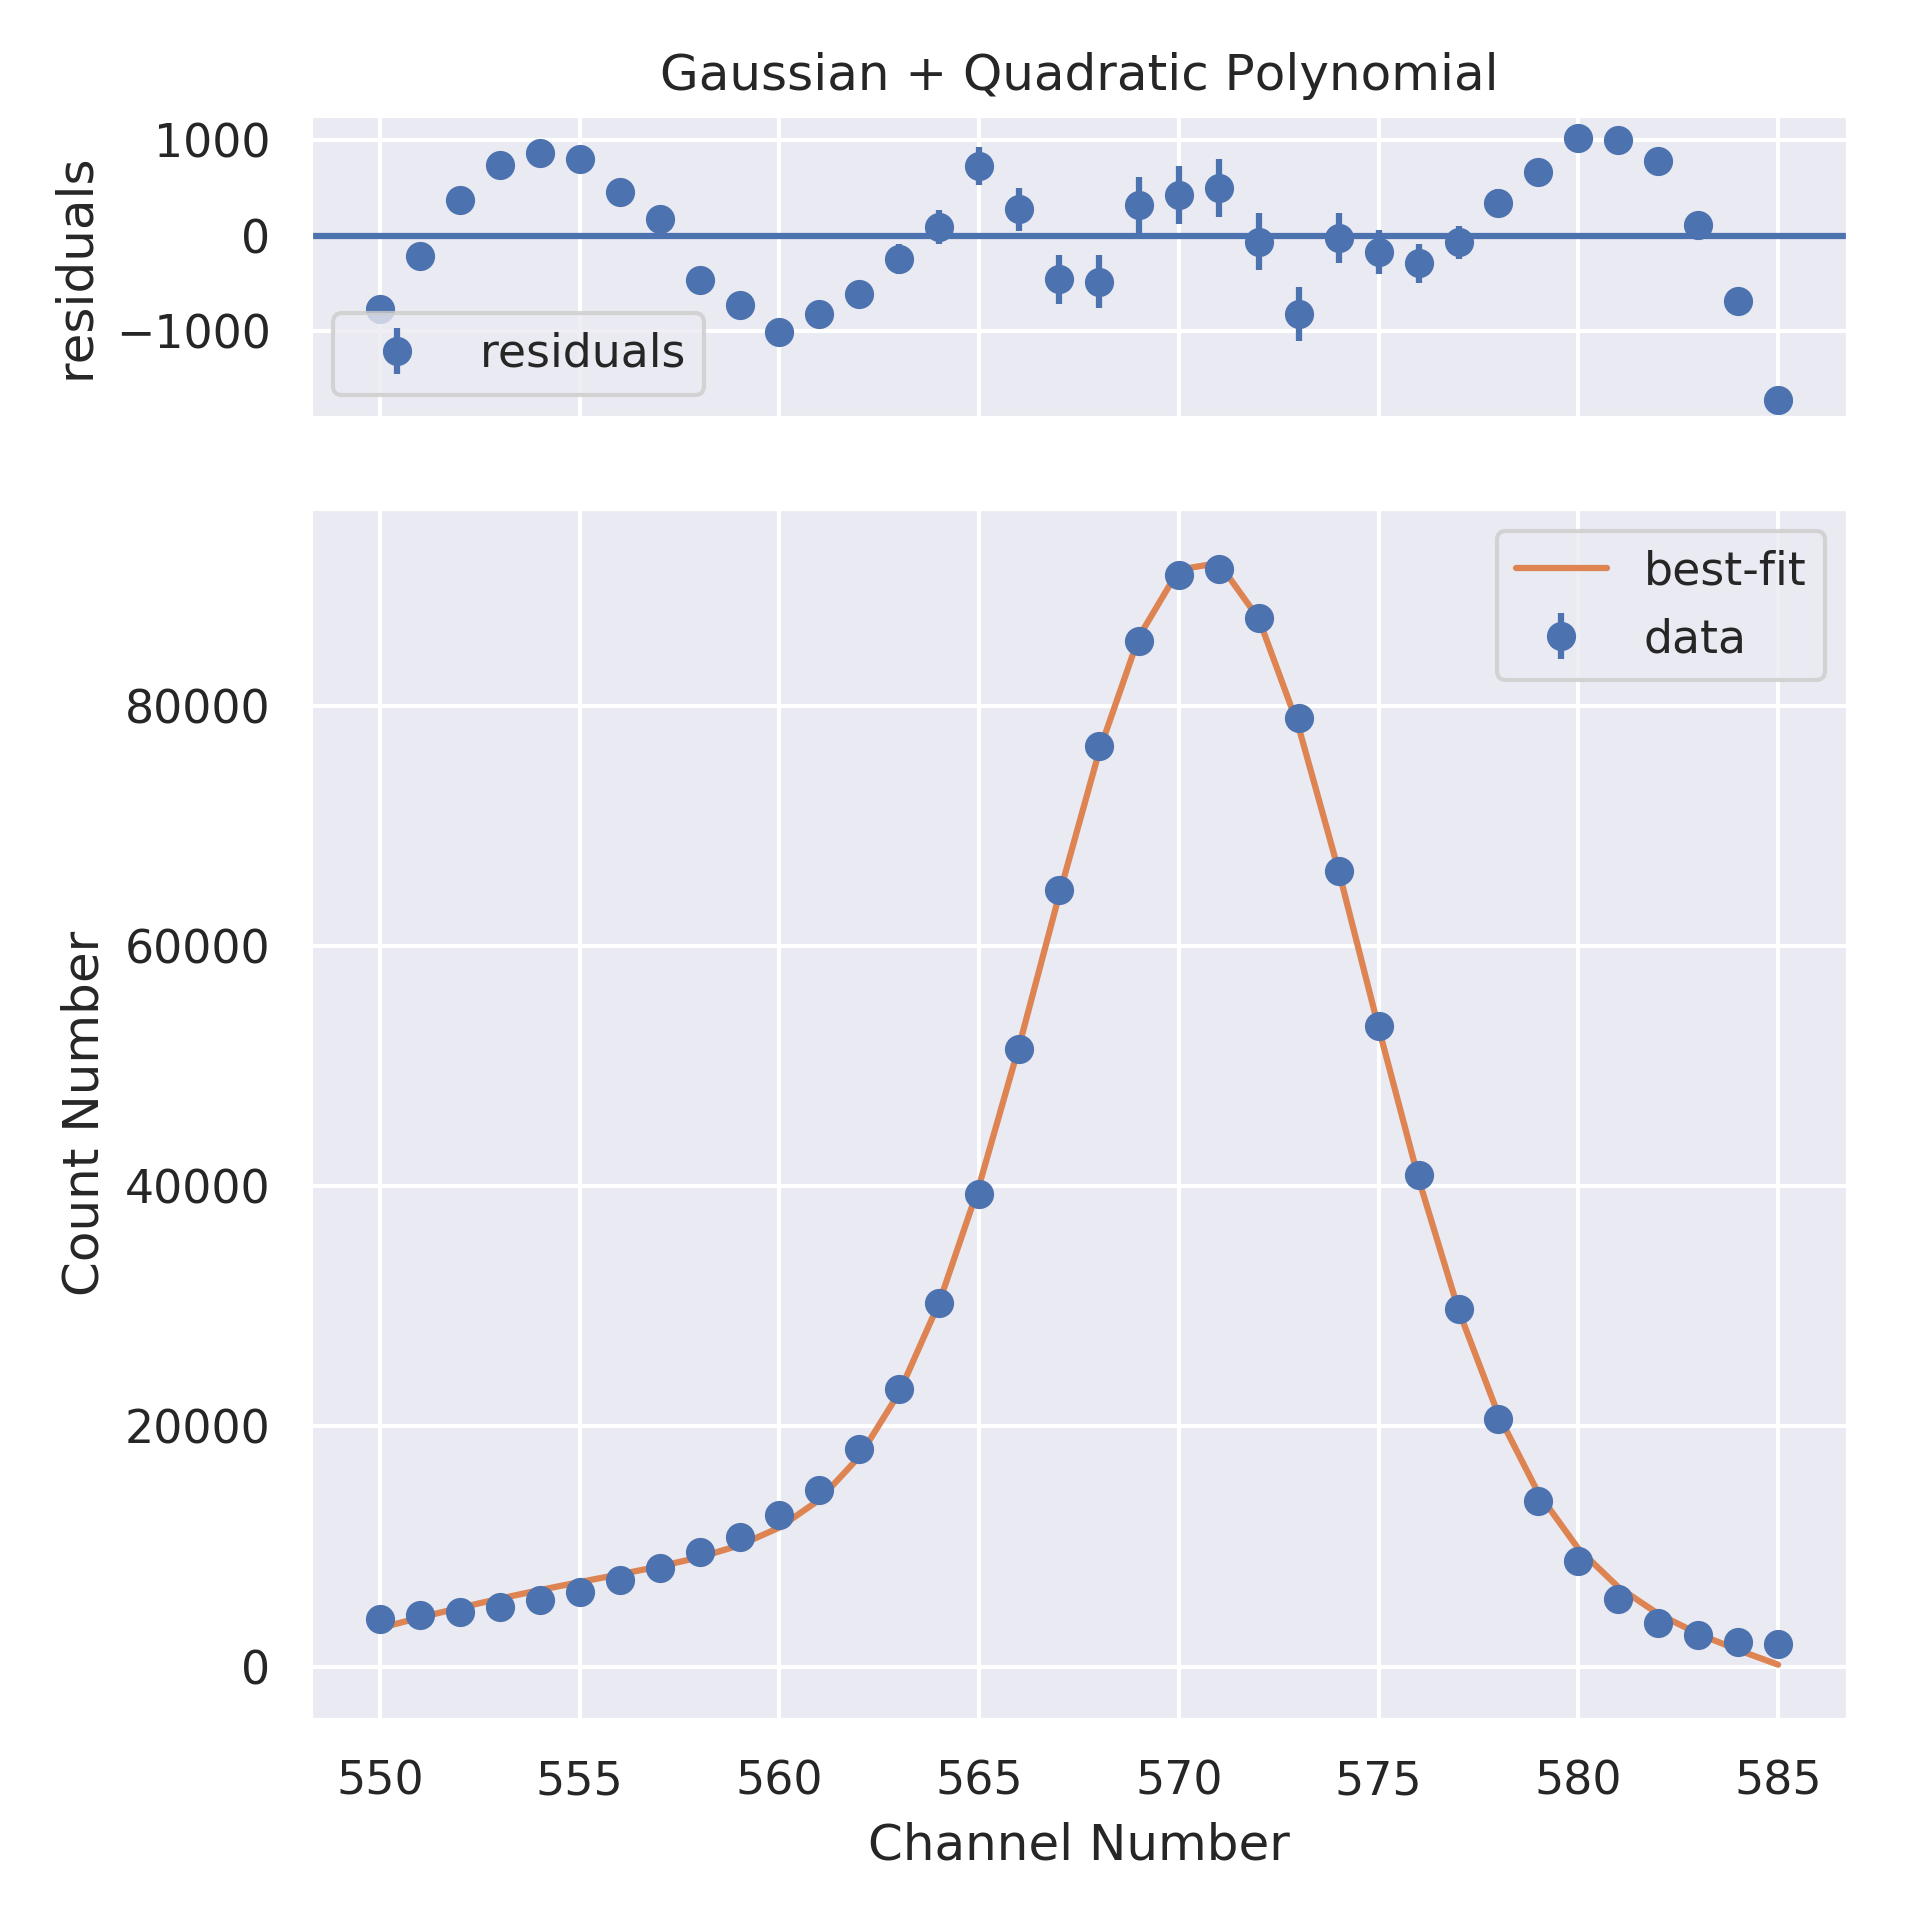
\includegraphics[width=\linewidth]{./Images/Barium133/Quad/Quad_1_Full.png}
    \caption{Full peak with fit. $\chi^2 = 3108.72$, $\chi^2_\nu = 91.43$, \\ Prob = 0\%, $\mu = 570.65$, $\sigma = 3.96$}
    %\label{fig:sub1}
  \end{subfigure}%
  \begin{subfigure}{.5\linewidth}
    \centering
    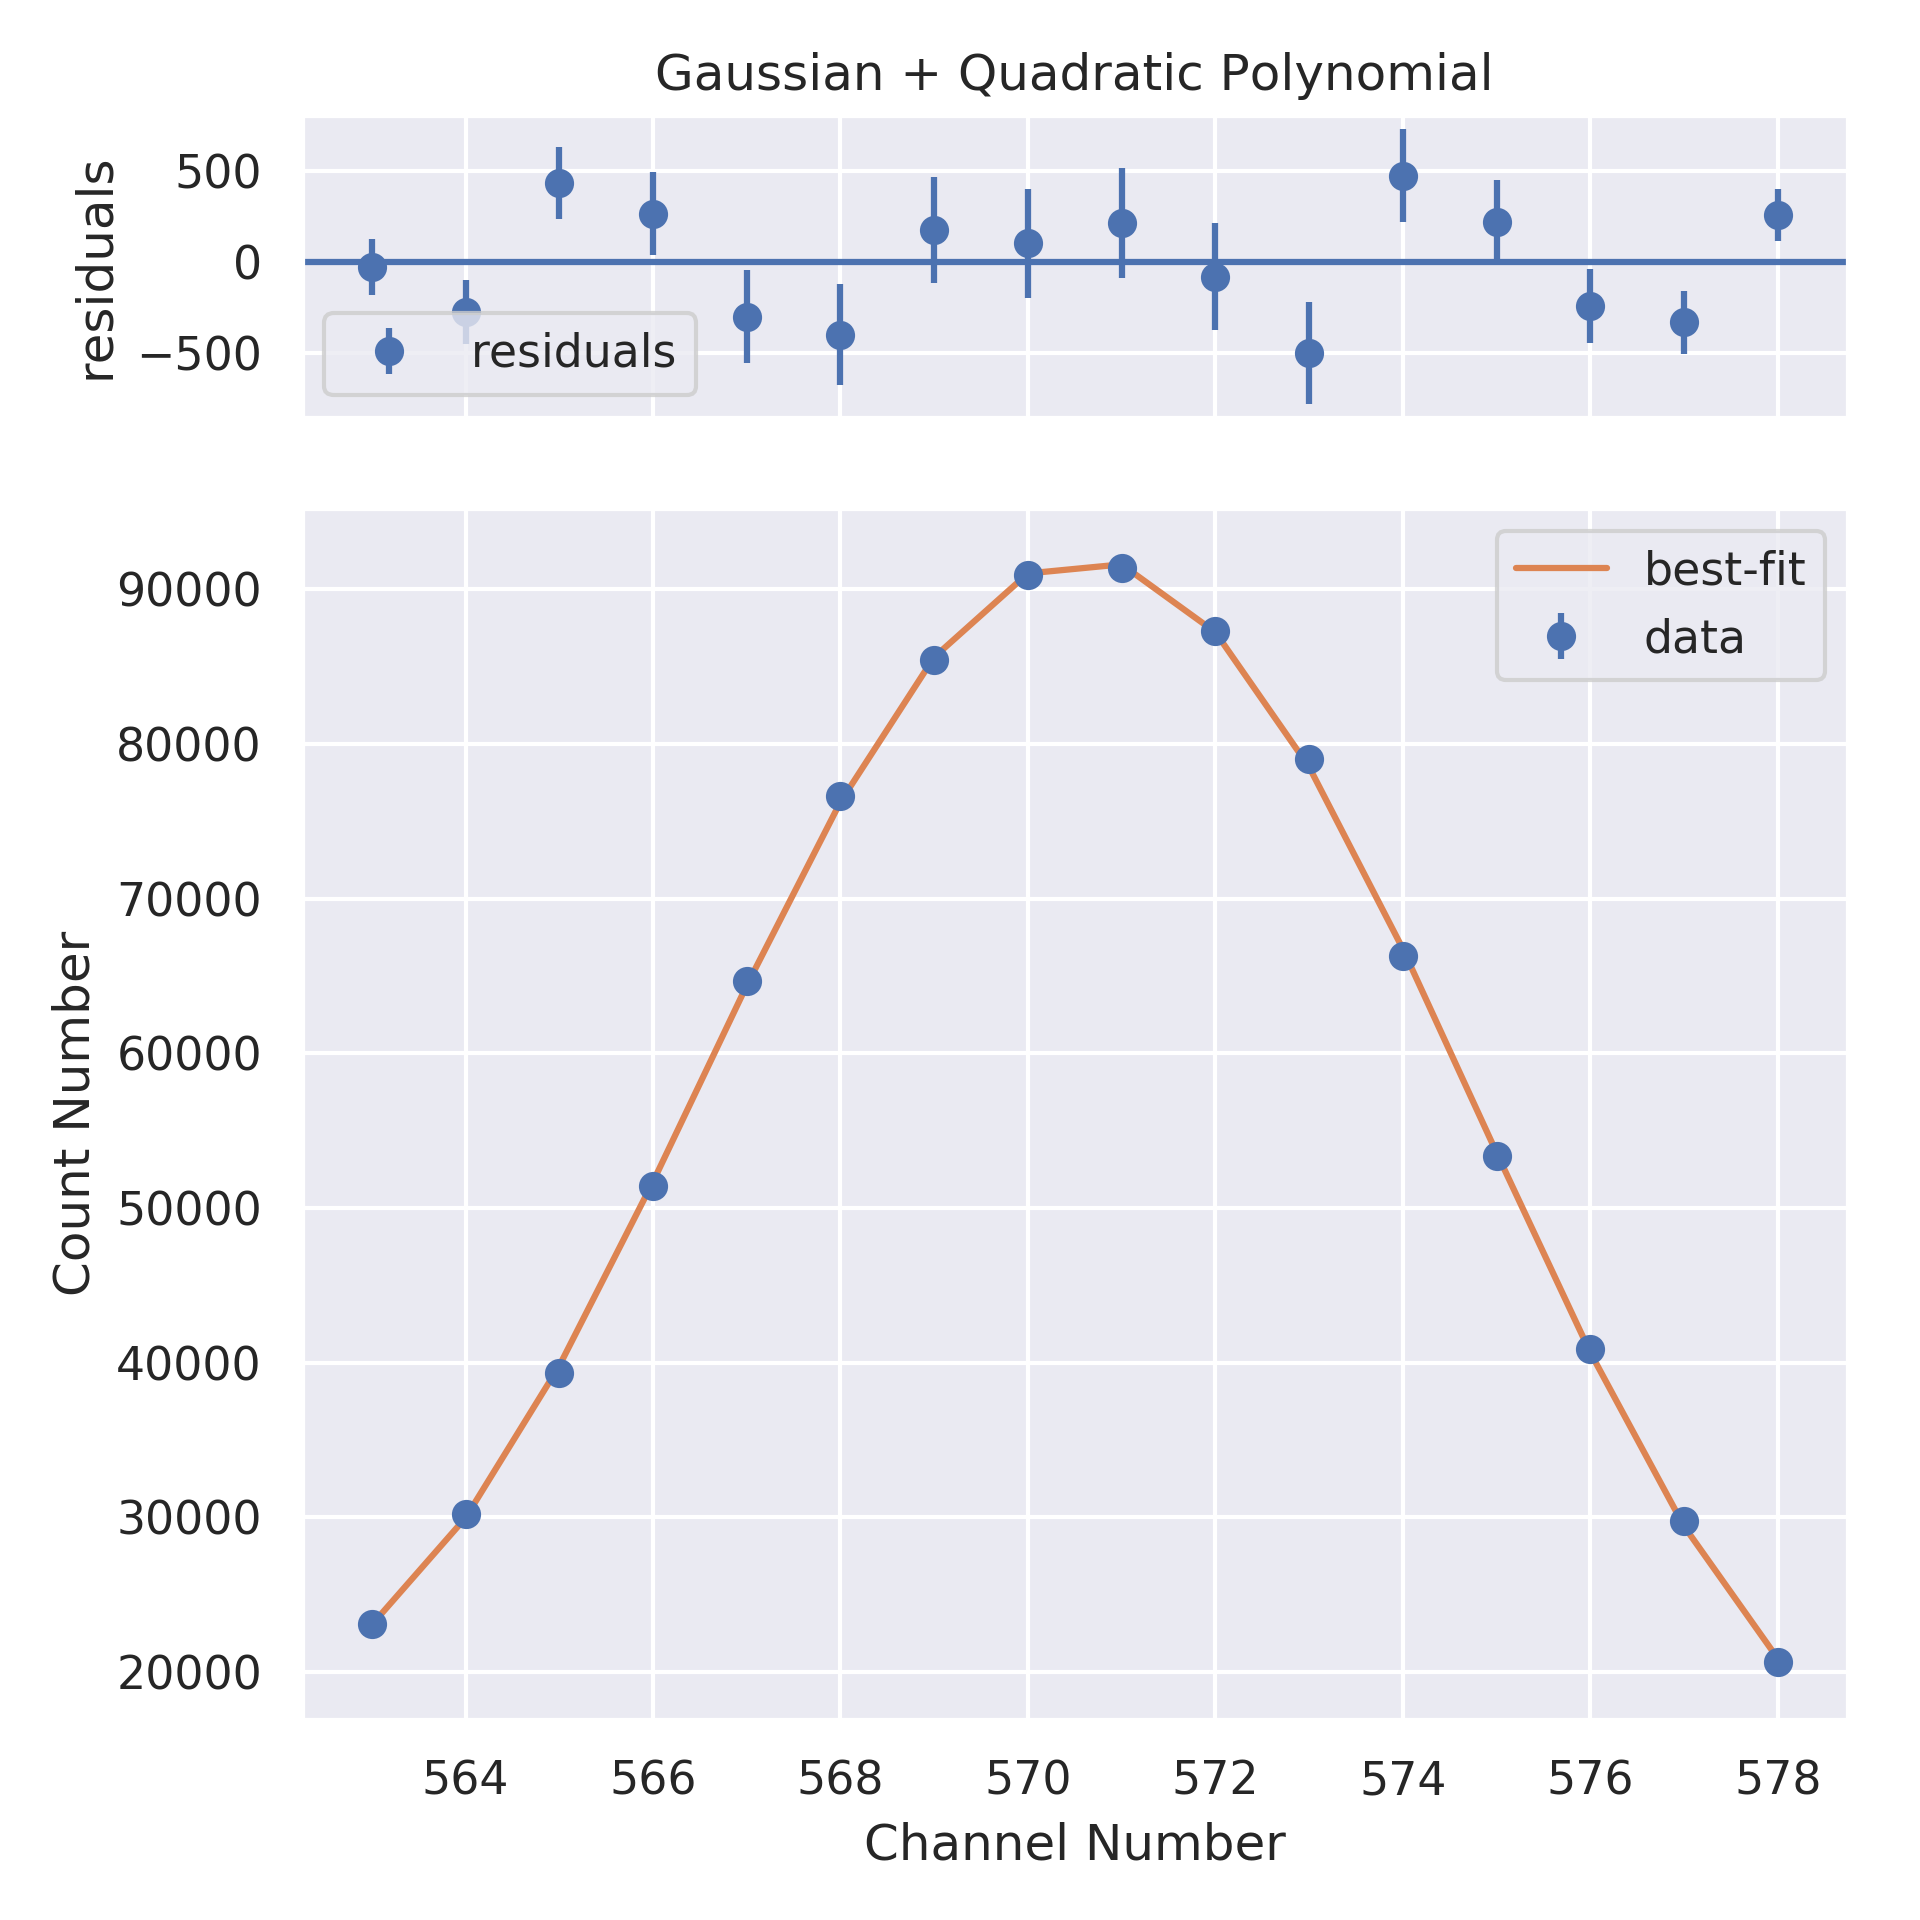
\includegraphics[width=\linewidth]{./Images/Barium133/Quad/Quad_1_Zoom.png}
    \caption{Zoomed in peak with fit. $\chi^2 = 29.06$, $\chi^2_\nu = 2.08$, \\ Prob = 1.03\%, $\mu = 570.67$, $\sigma = 4.61$}
    %\label{fig:sub2}
  \end{subfigure}
  \caption{Fit of full \& zoomed in peak of \element{Ba}{133} 81 keV peak}
  %\label{fig:test}
\end{figure}
\begin{figure}[H]
  \centering
  \begin{subfigure}{.5\linewidth}
    \centering
    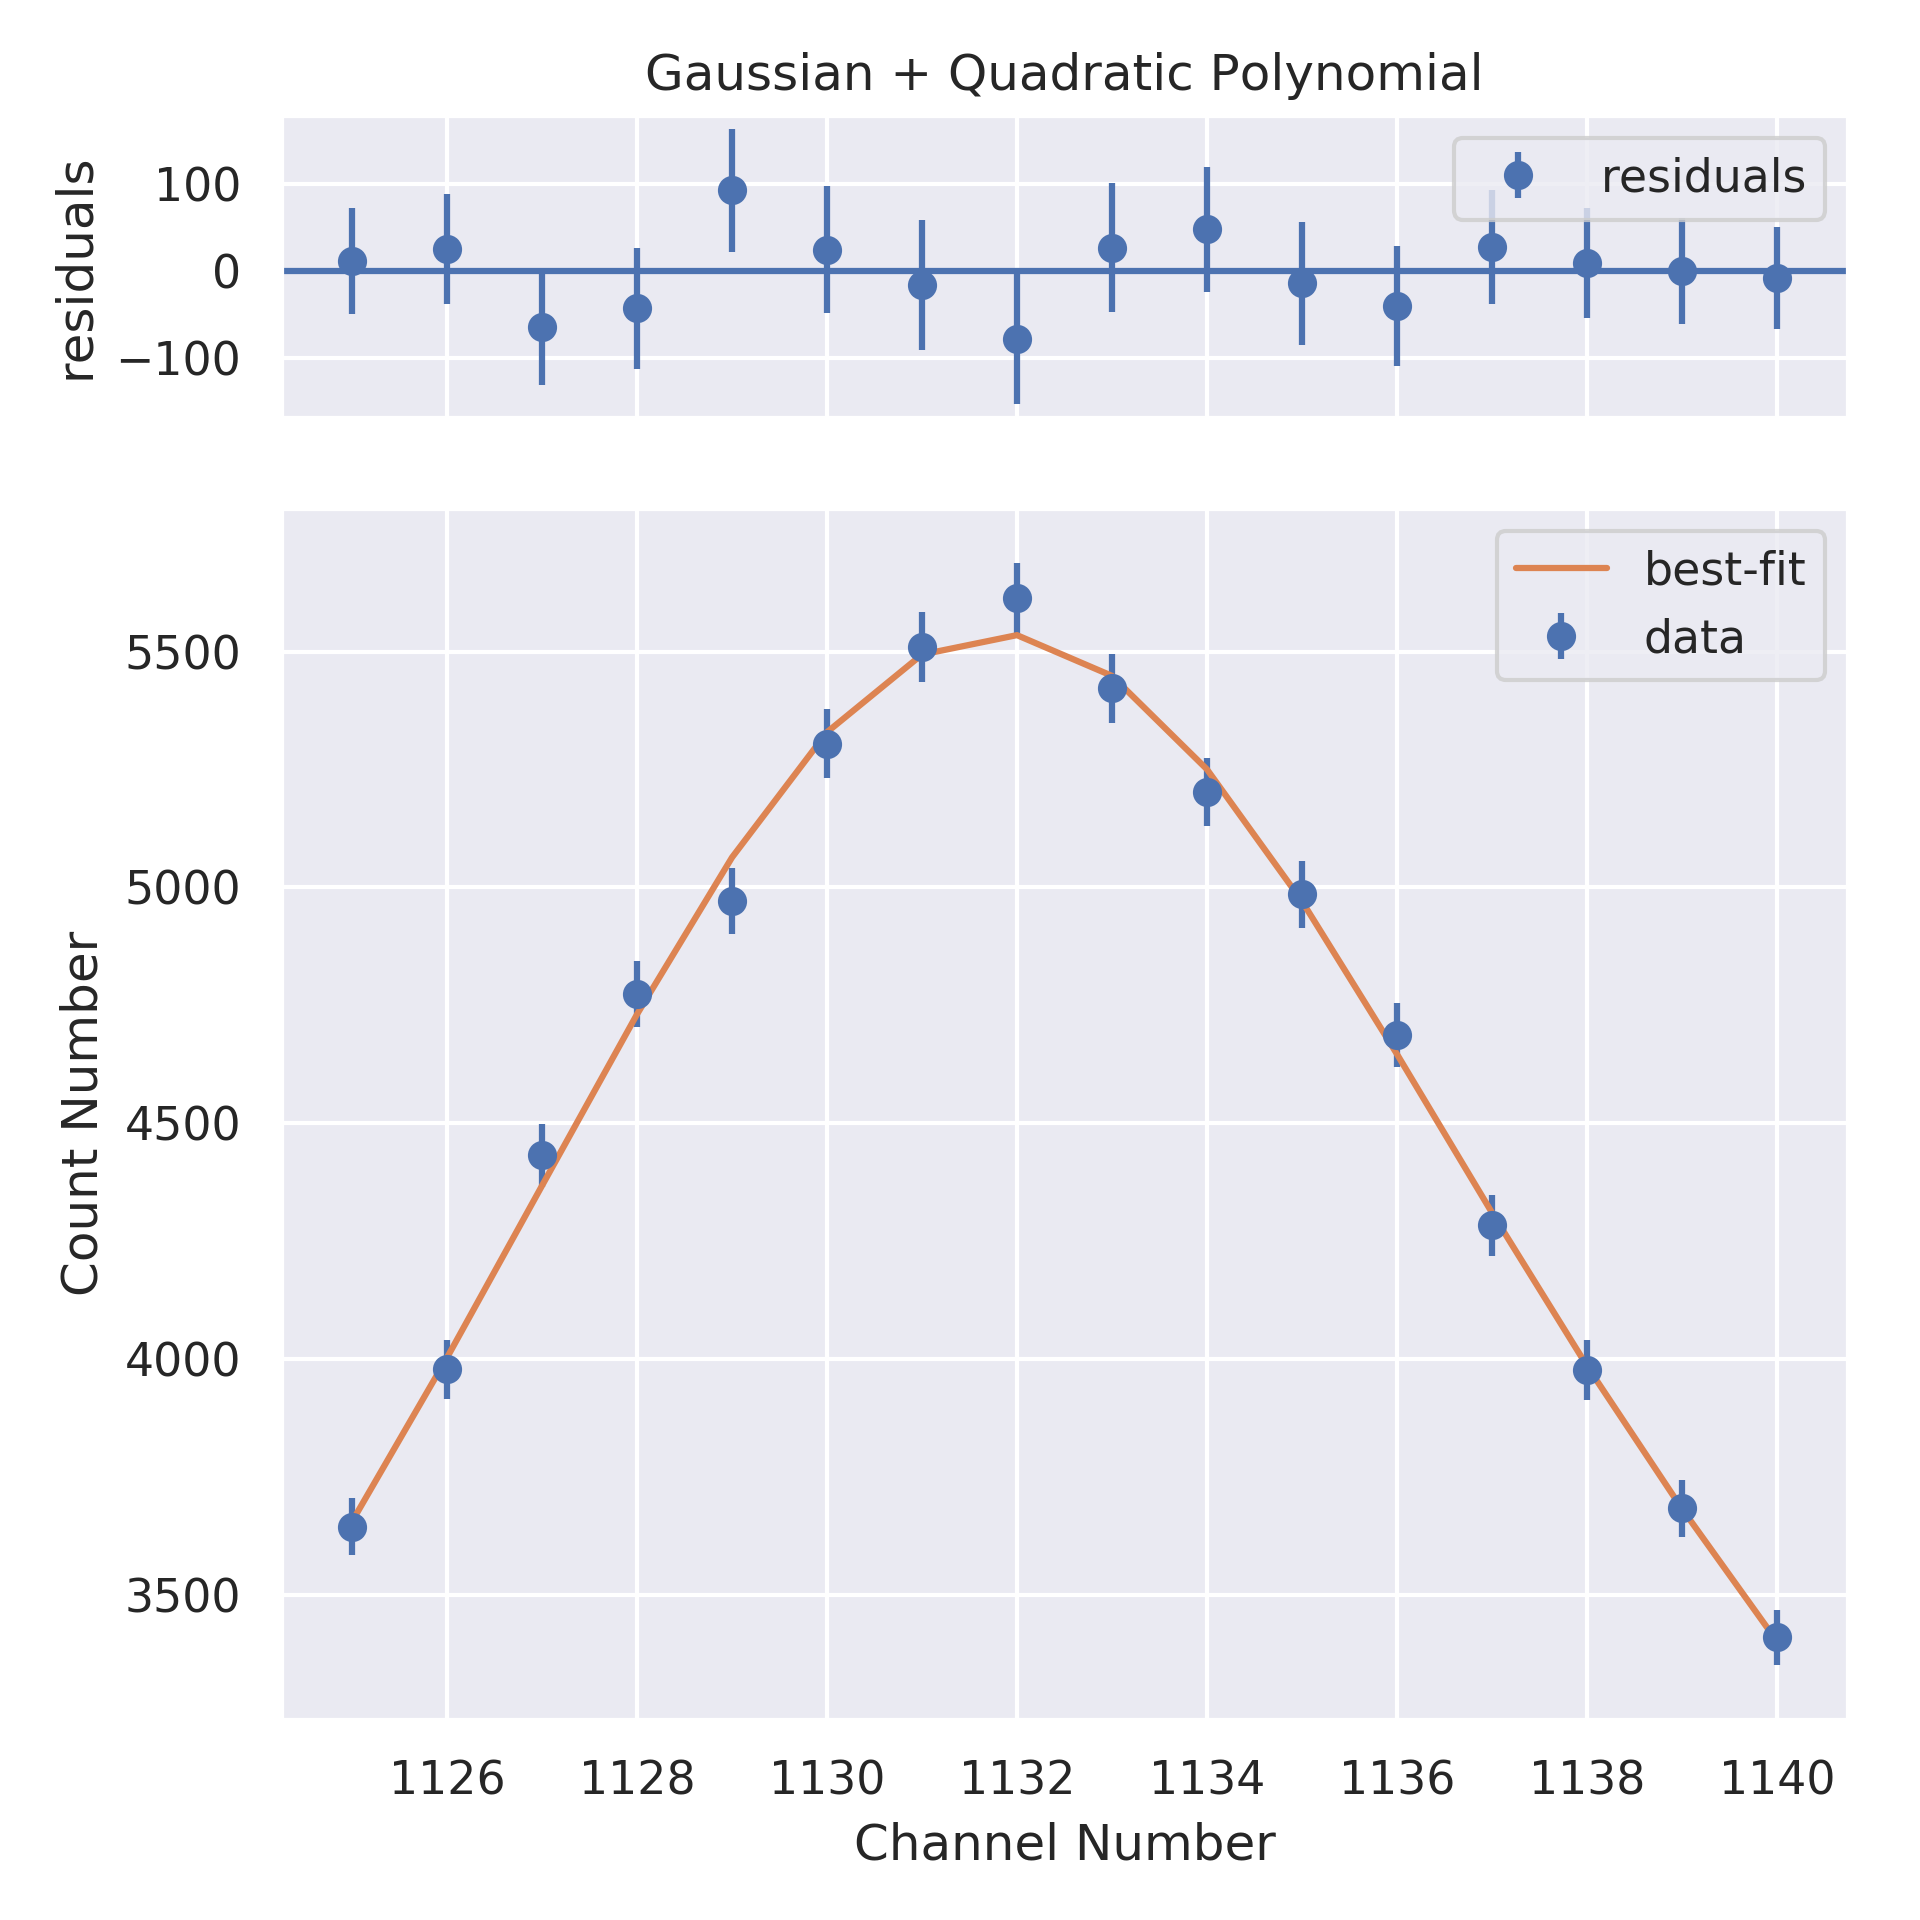
\includegraphics[width=\linewidth]{./Images/Barium133/Quad/Quad_2_Full.png}
    \caption{Full peak with fit. $\chi^2 = 5.65$, $\chi^2_\nu = 0.40$, \\ Prob = 97.45\%, $\mu = 1131.70$, $\sigma = 3.89$}
    %\label{fig:sub1}
  \end{subfigure}%
  \begin{subfigure}{.5\linewidth}
    \centering
    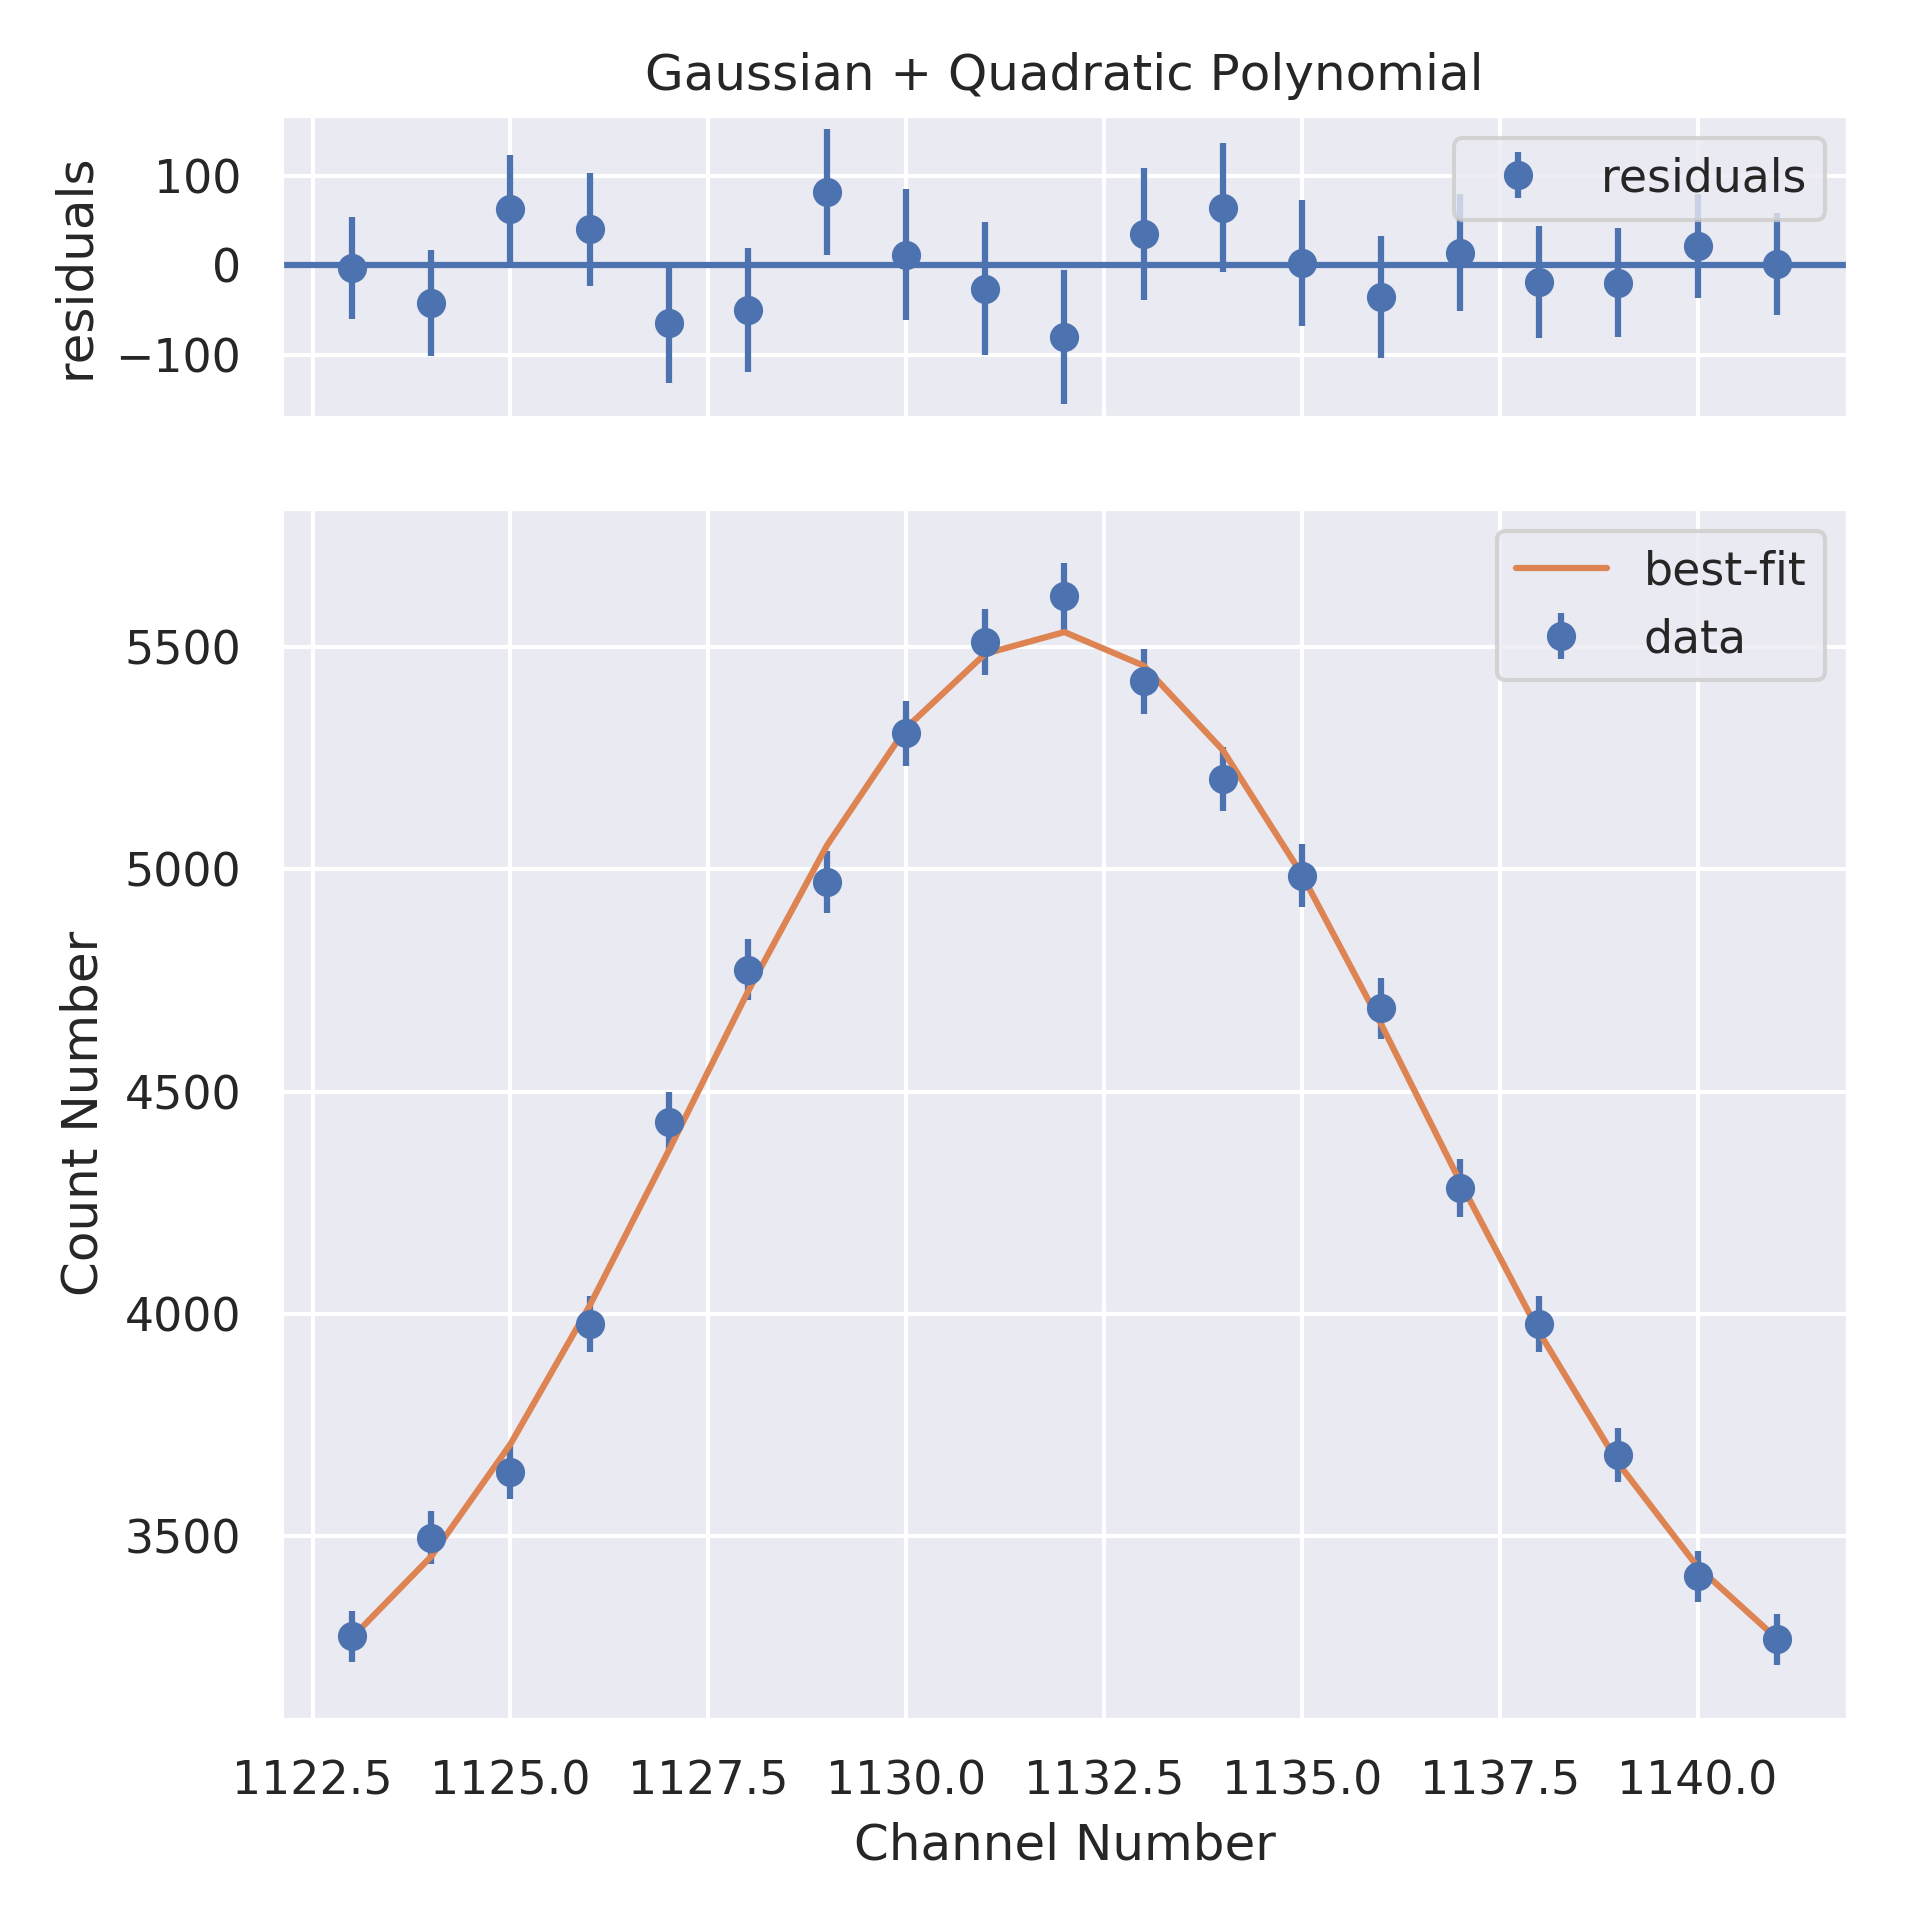
\includegraphics[width=\linewidth]{./Images/Barium133/Quad/Quad_2_Zoom.png}
    \caption{Zoomed in peak with fit. $\chi^2 = 7.80$, $\chi^2_\nu = 0.46$, \\ Prob = 97.07\%, $\mu = 1131.88$, $\sigma = 4.69$}
    %\label{fig:sub2}
  \end{subfigure}
  \caption{Fit of full \& zoomed in peak of \element{Ba}{133} 161 keV peak}
  %\label{fig:test}
\end{figure}
\begin{figure}[H]
  \centering
  \begin{subfigure}{.5\linewidth}
    \centering
    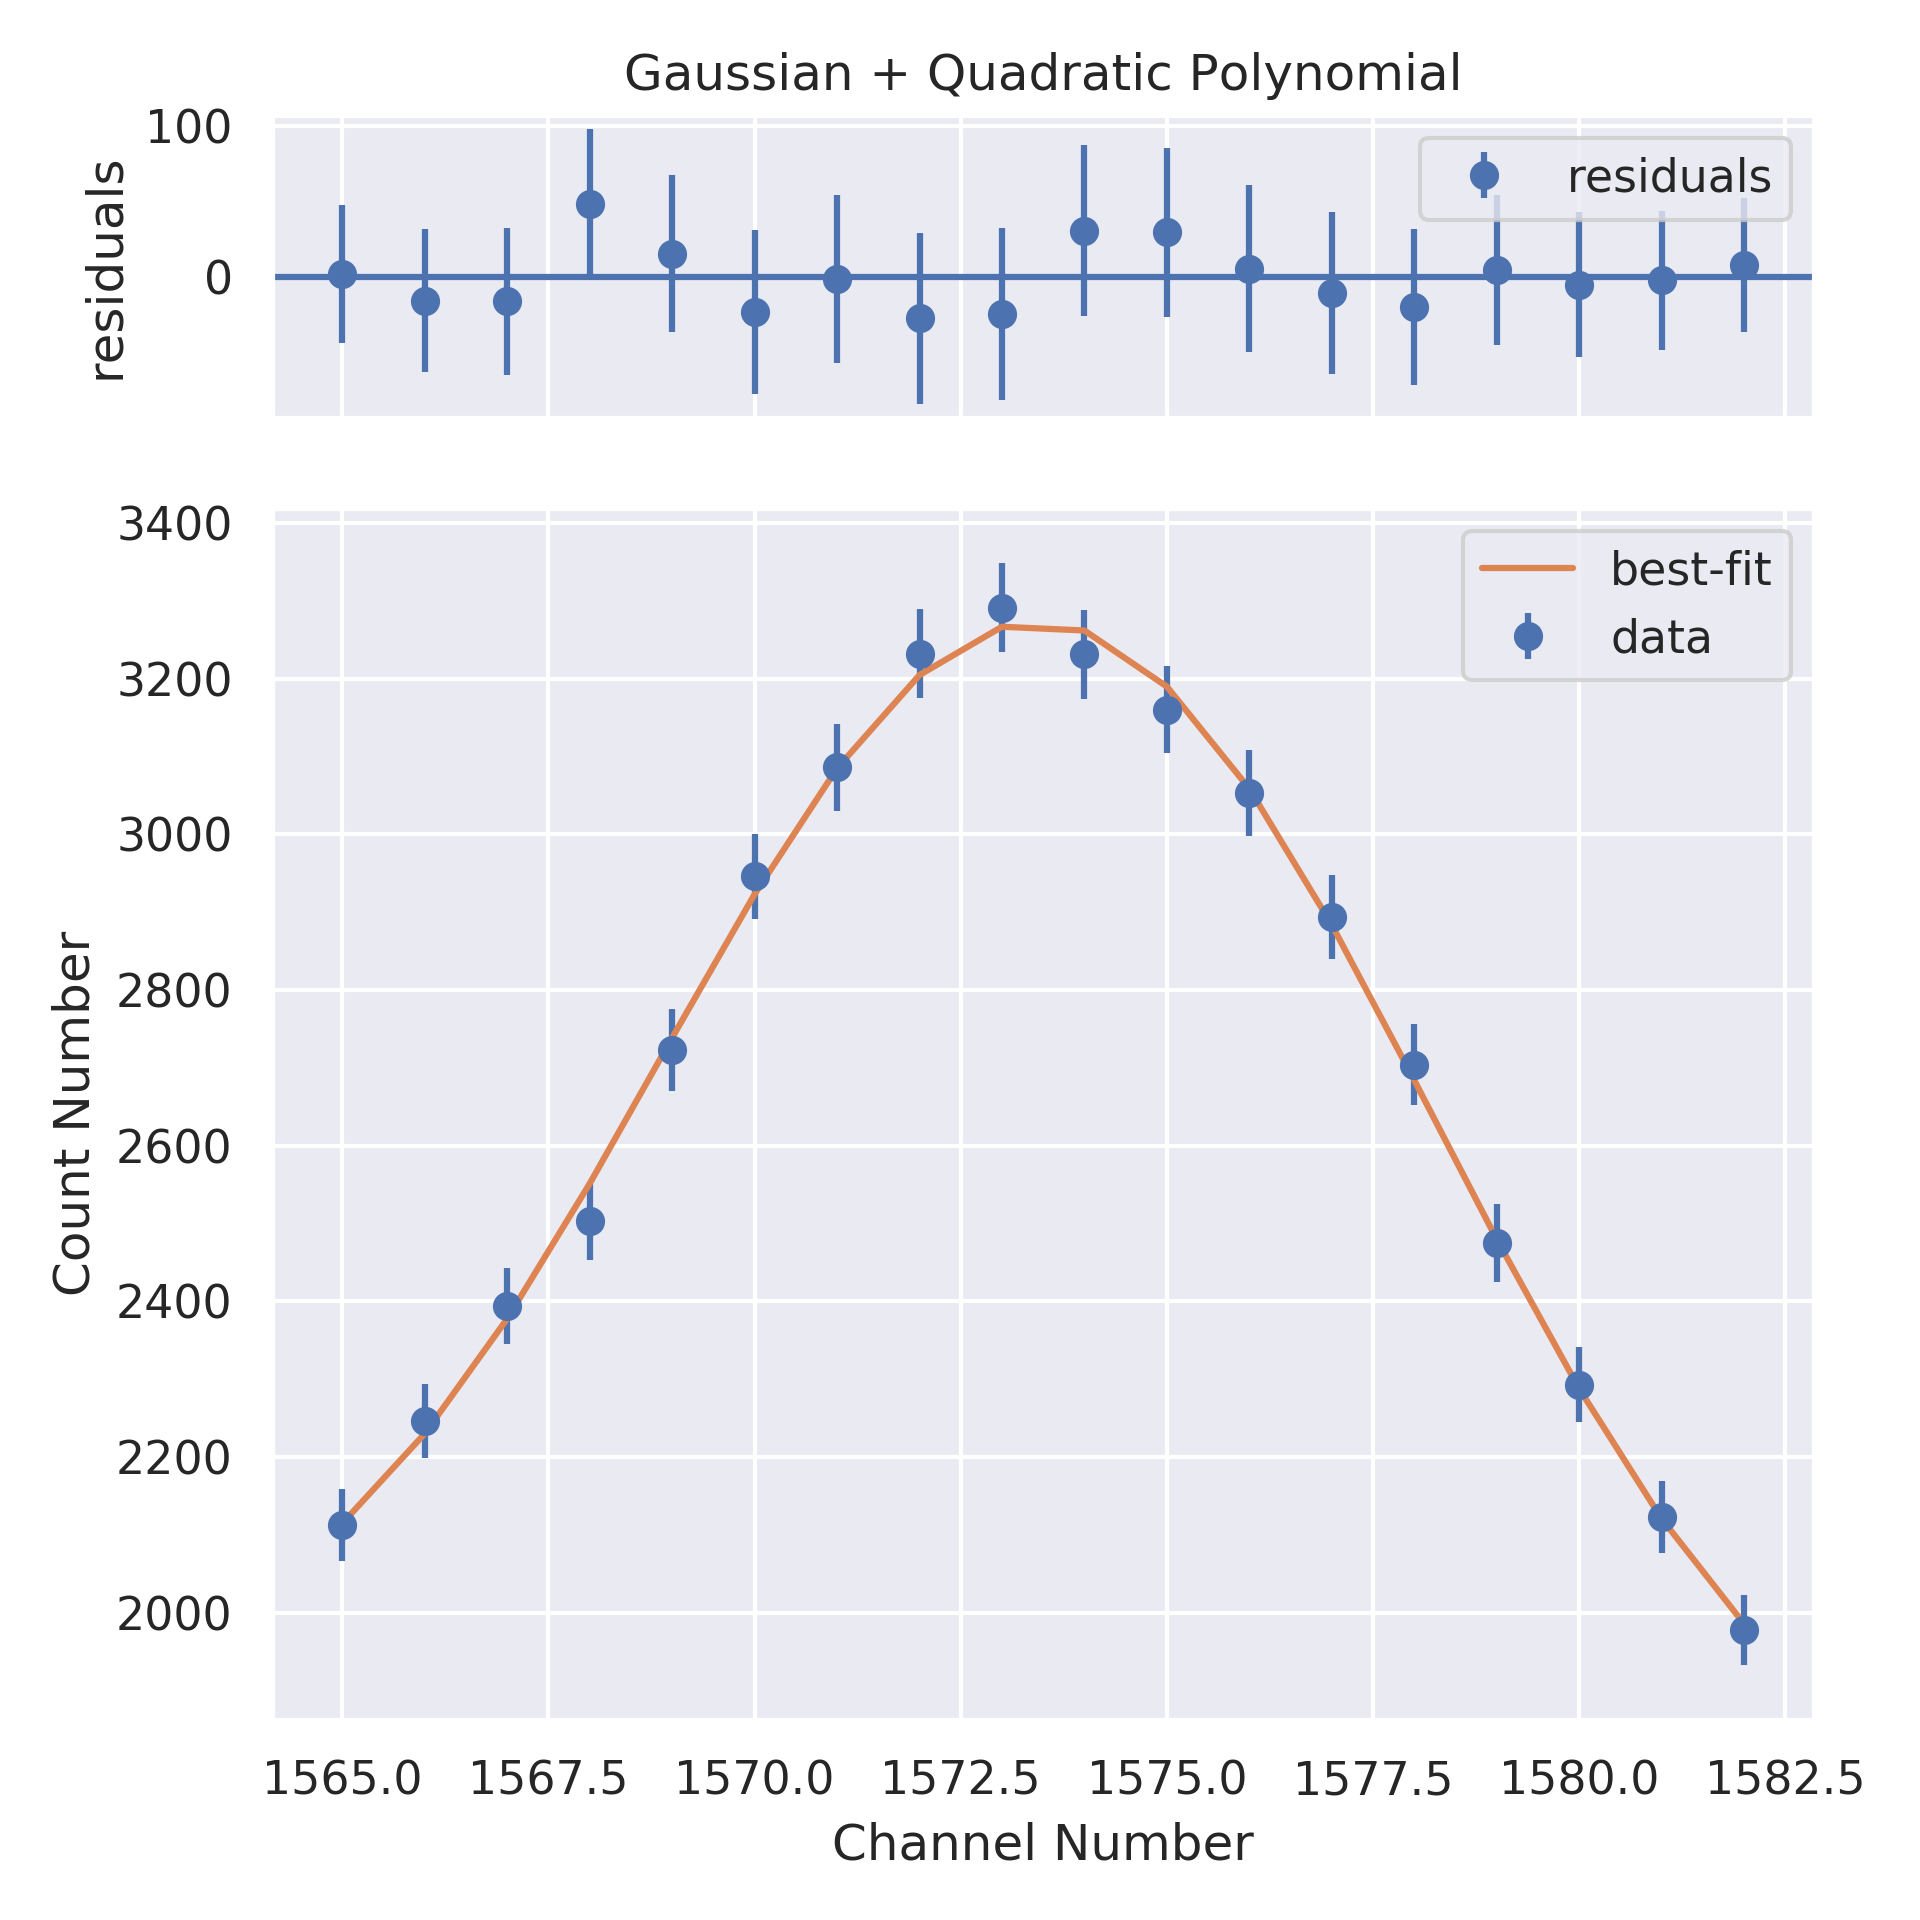
\includegraphics[width=\linewidth]{./Images/Barium133/Quad/Quad_3_Full.png}
    \caption{Full peak with fit. $\chi^2 = 2.66$, $\chi^2_\nu = 0.17$, \\ Prob = 99.99\%, $\mu = 1573.55$, $\sigma = 4.82$}
    %\label{fig:sub1}
  \end{subfigure}%
  \begin{subfigure}{.5\linewidth}
    \centering
    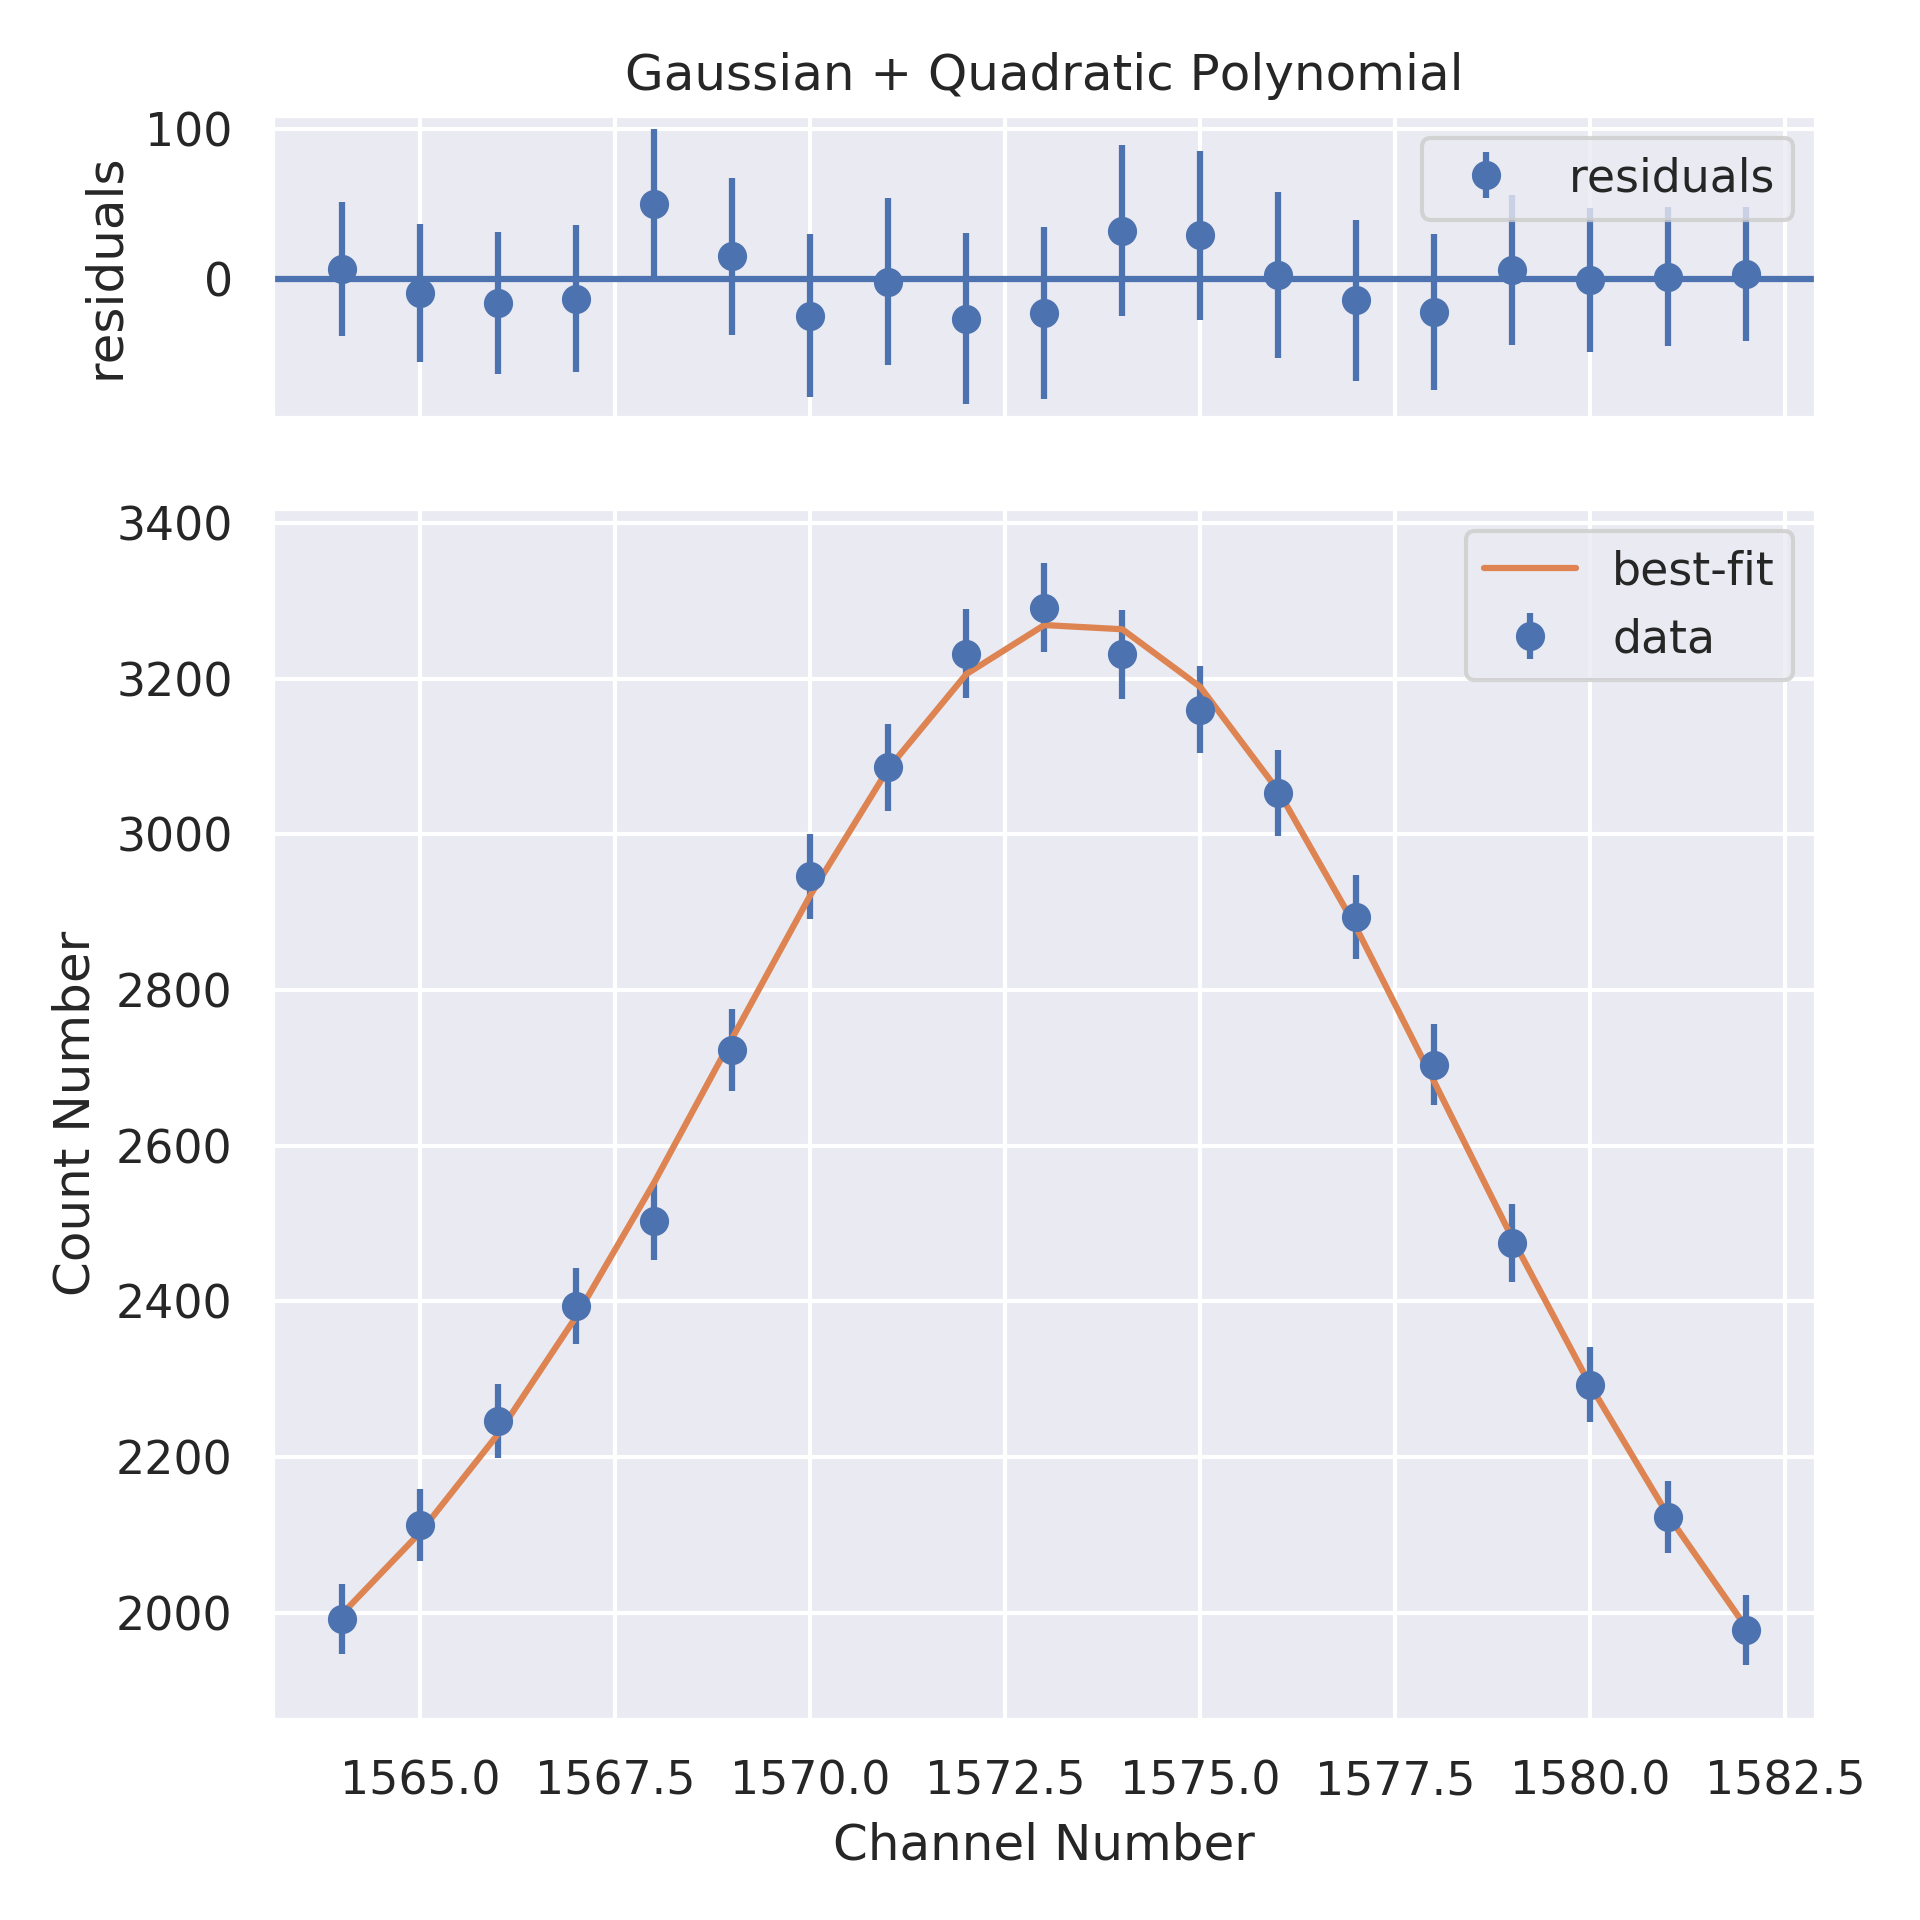
\includegraphics[width=\linewidth]{./Images/Barium133/Quad/Quad_3_Zoom.png}
    \caption{Zoomed in peak with fit. $\chi^2 = 2.77$, $\chi^2_\nu = 0.16$, \\ Prob = 100\%, $\mu = 1573.53$, $\sigma = 4.34$}
    %\label{fig:sub2}
  \end{subfigure}
  \caption{Fit of full \& zoomed in peak of \element{Ba}{133} 223 keV peak}
  %\label{fig:test}
\end{figure}
\begin{figure}[H]
  \centering
  \begin{subfigure}{.5\linewidth}
    \centering
    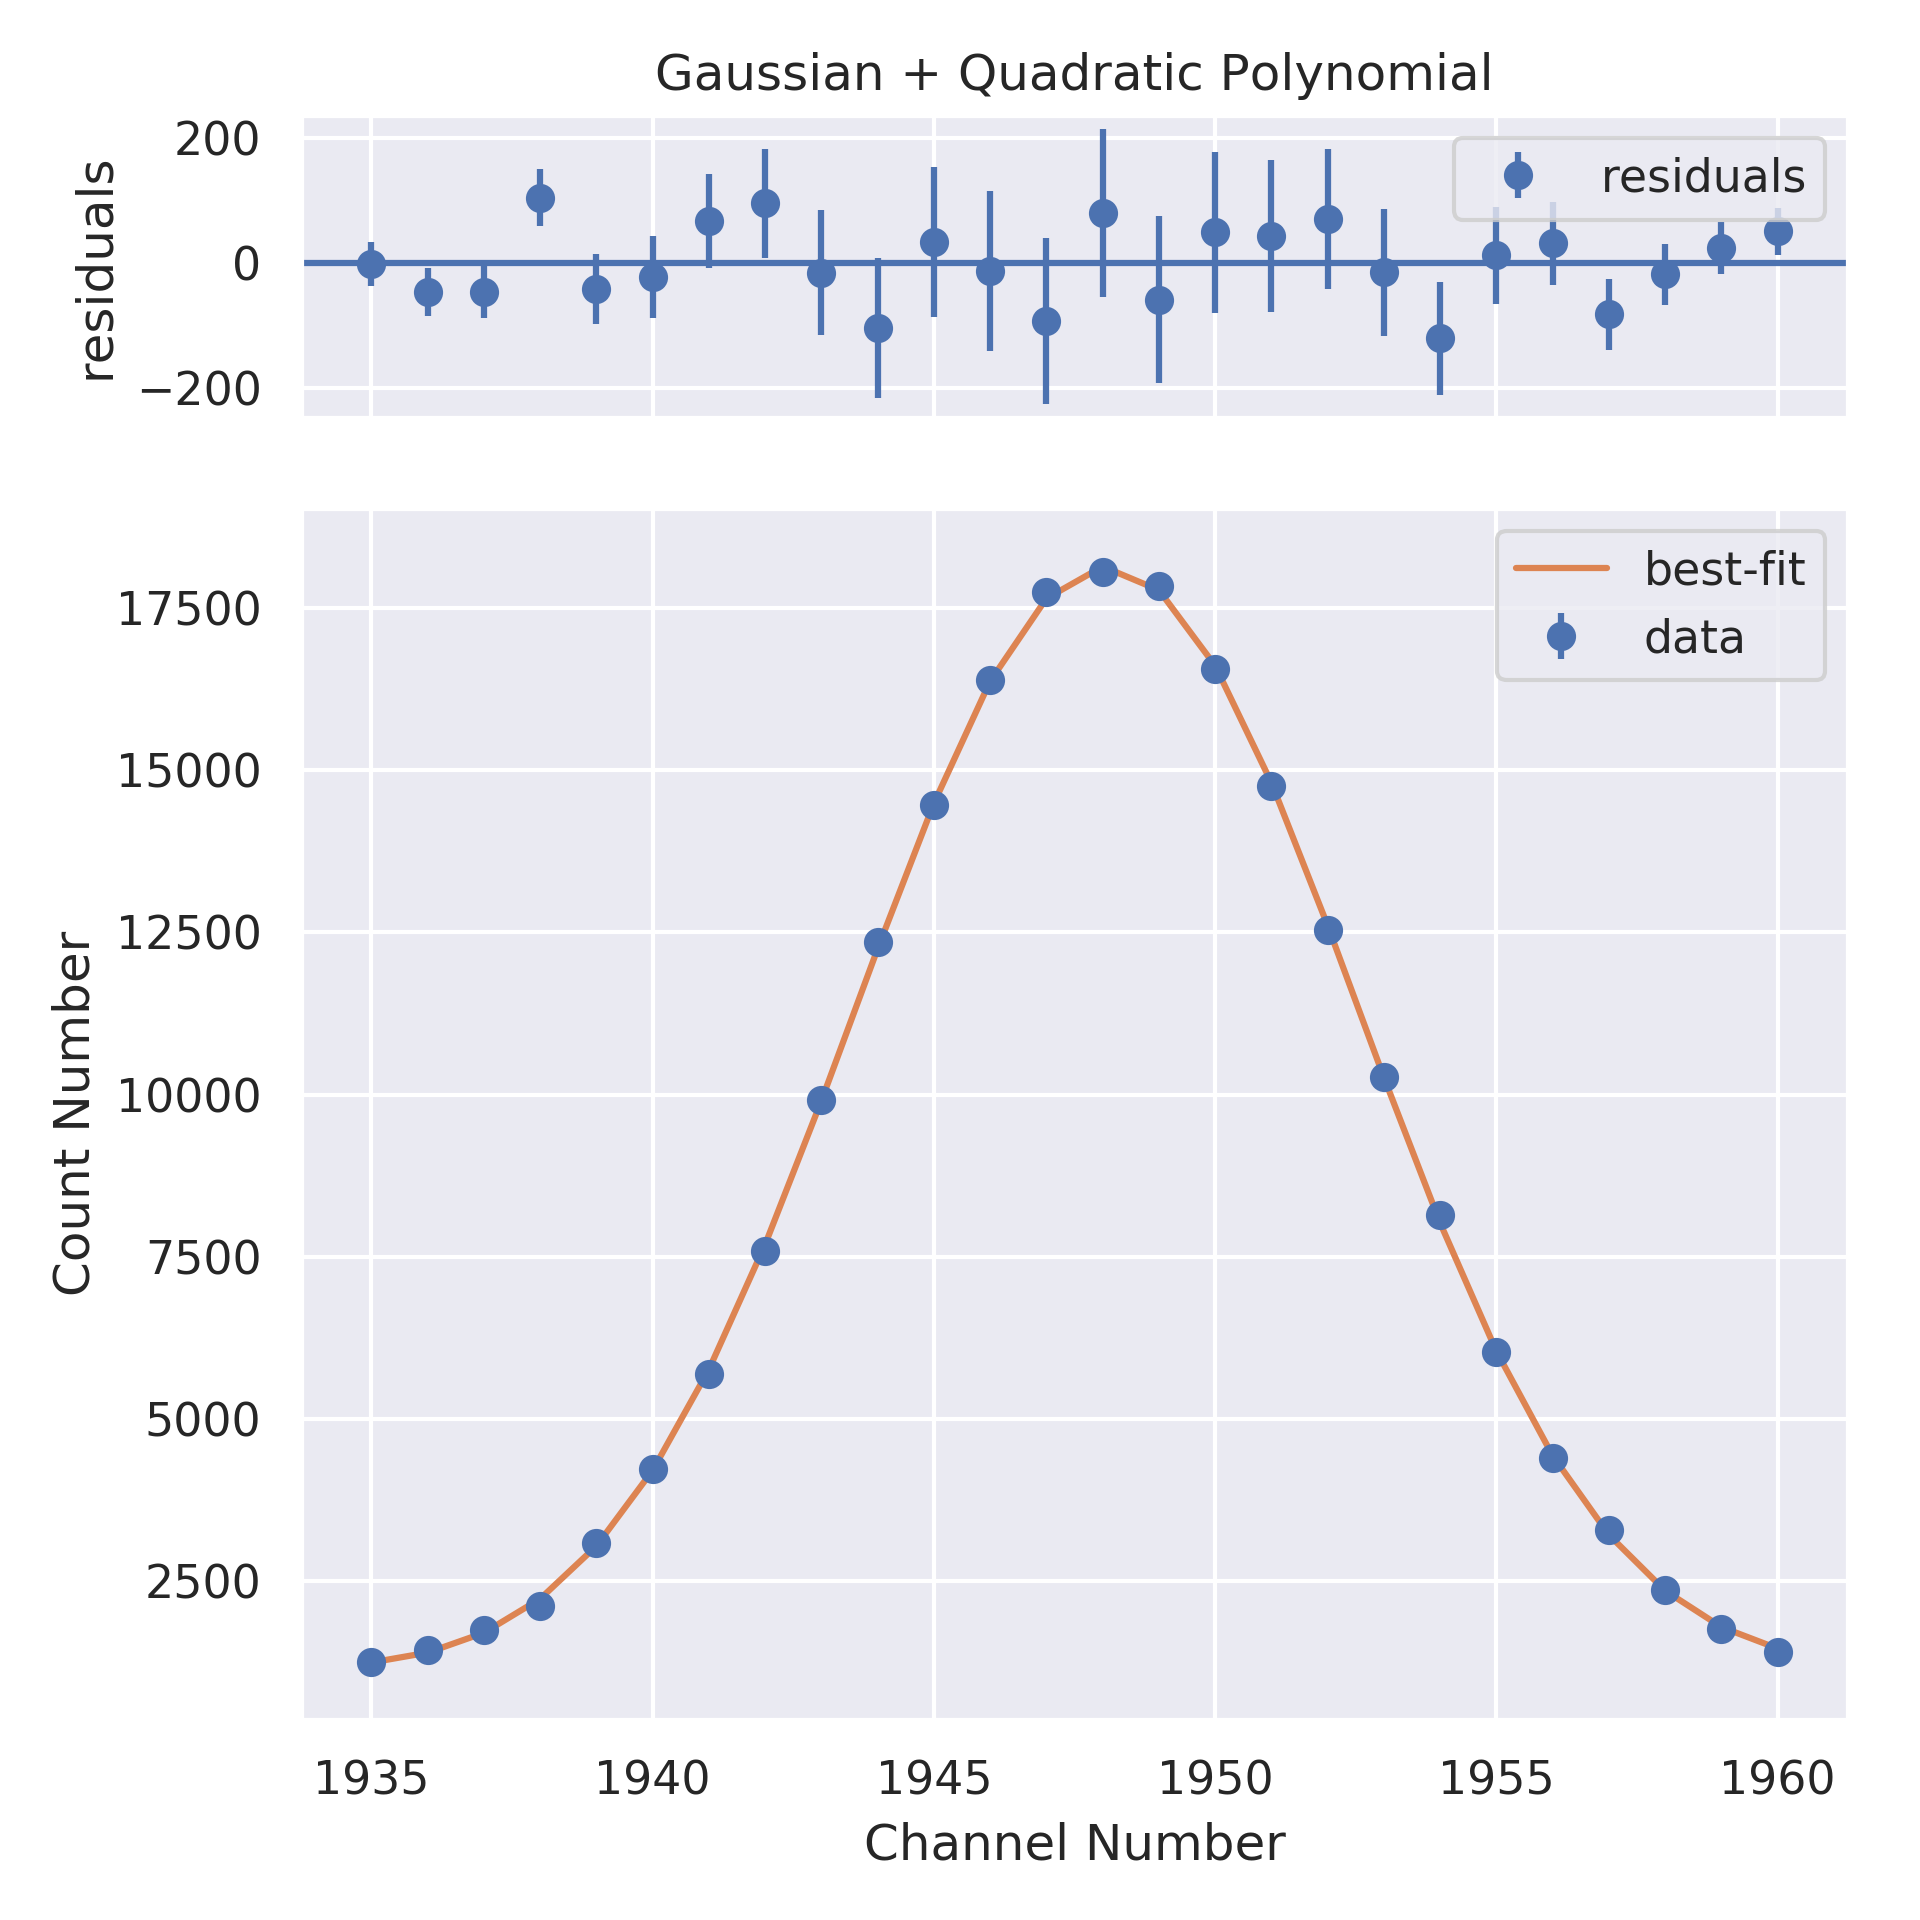
\includegraphics[width=\linewidth]{./Images/Barium133/Quad/Quad_4_Full.png}
    \caption{Full peak with fit. $\chi^2 = 19.63$, $\chi^2_\nu = 0.82$, \\ Prob = 71.76\%, $\mu = 1948.07$, $\sigma = 4.49$}
    %\label{fig:sub1}
  \end{subfigure}%
  \begin{subfigure}{.5\linewidth}
    \centering
    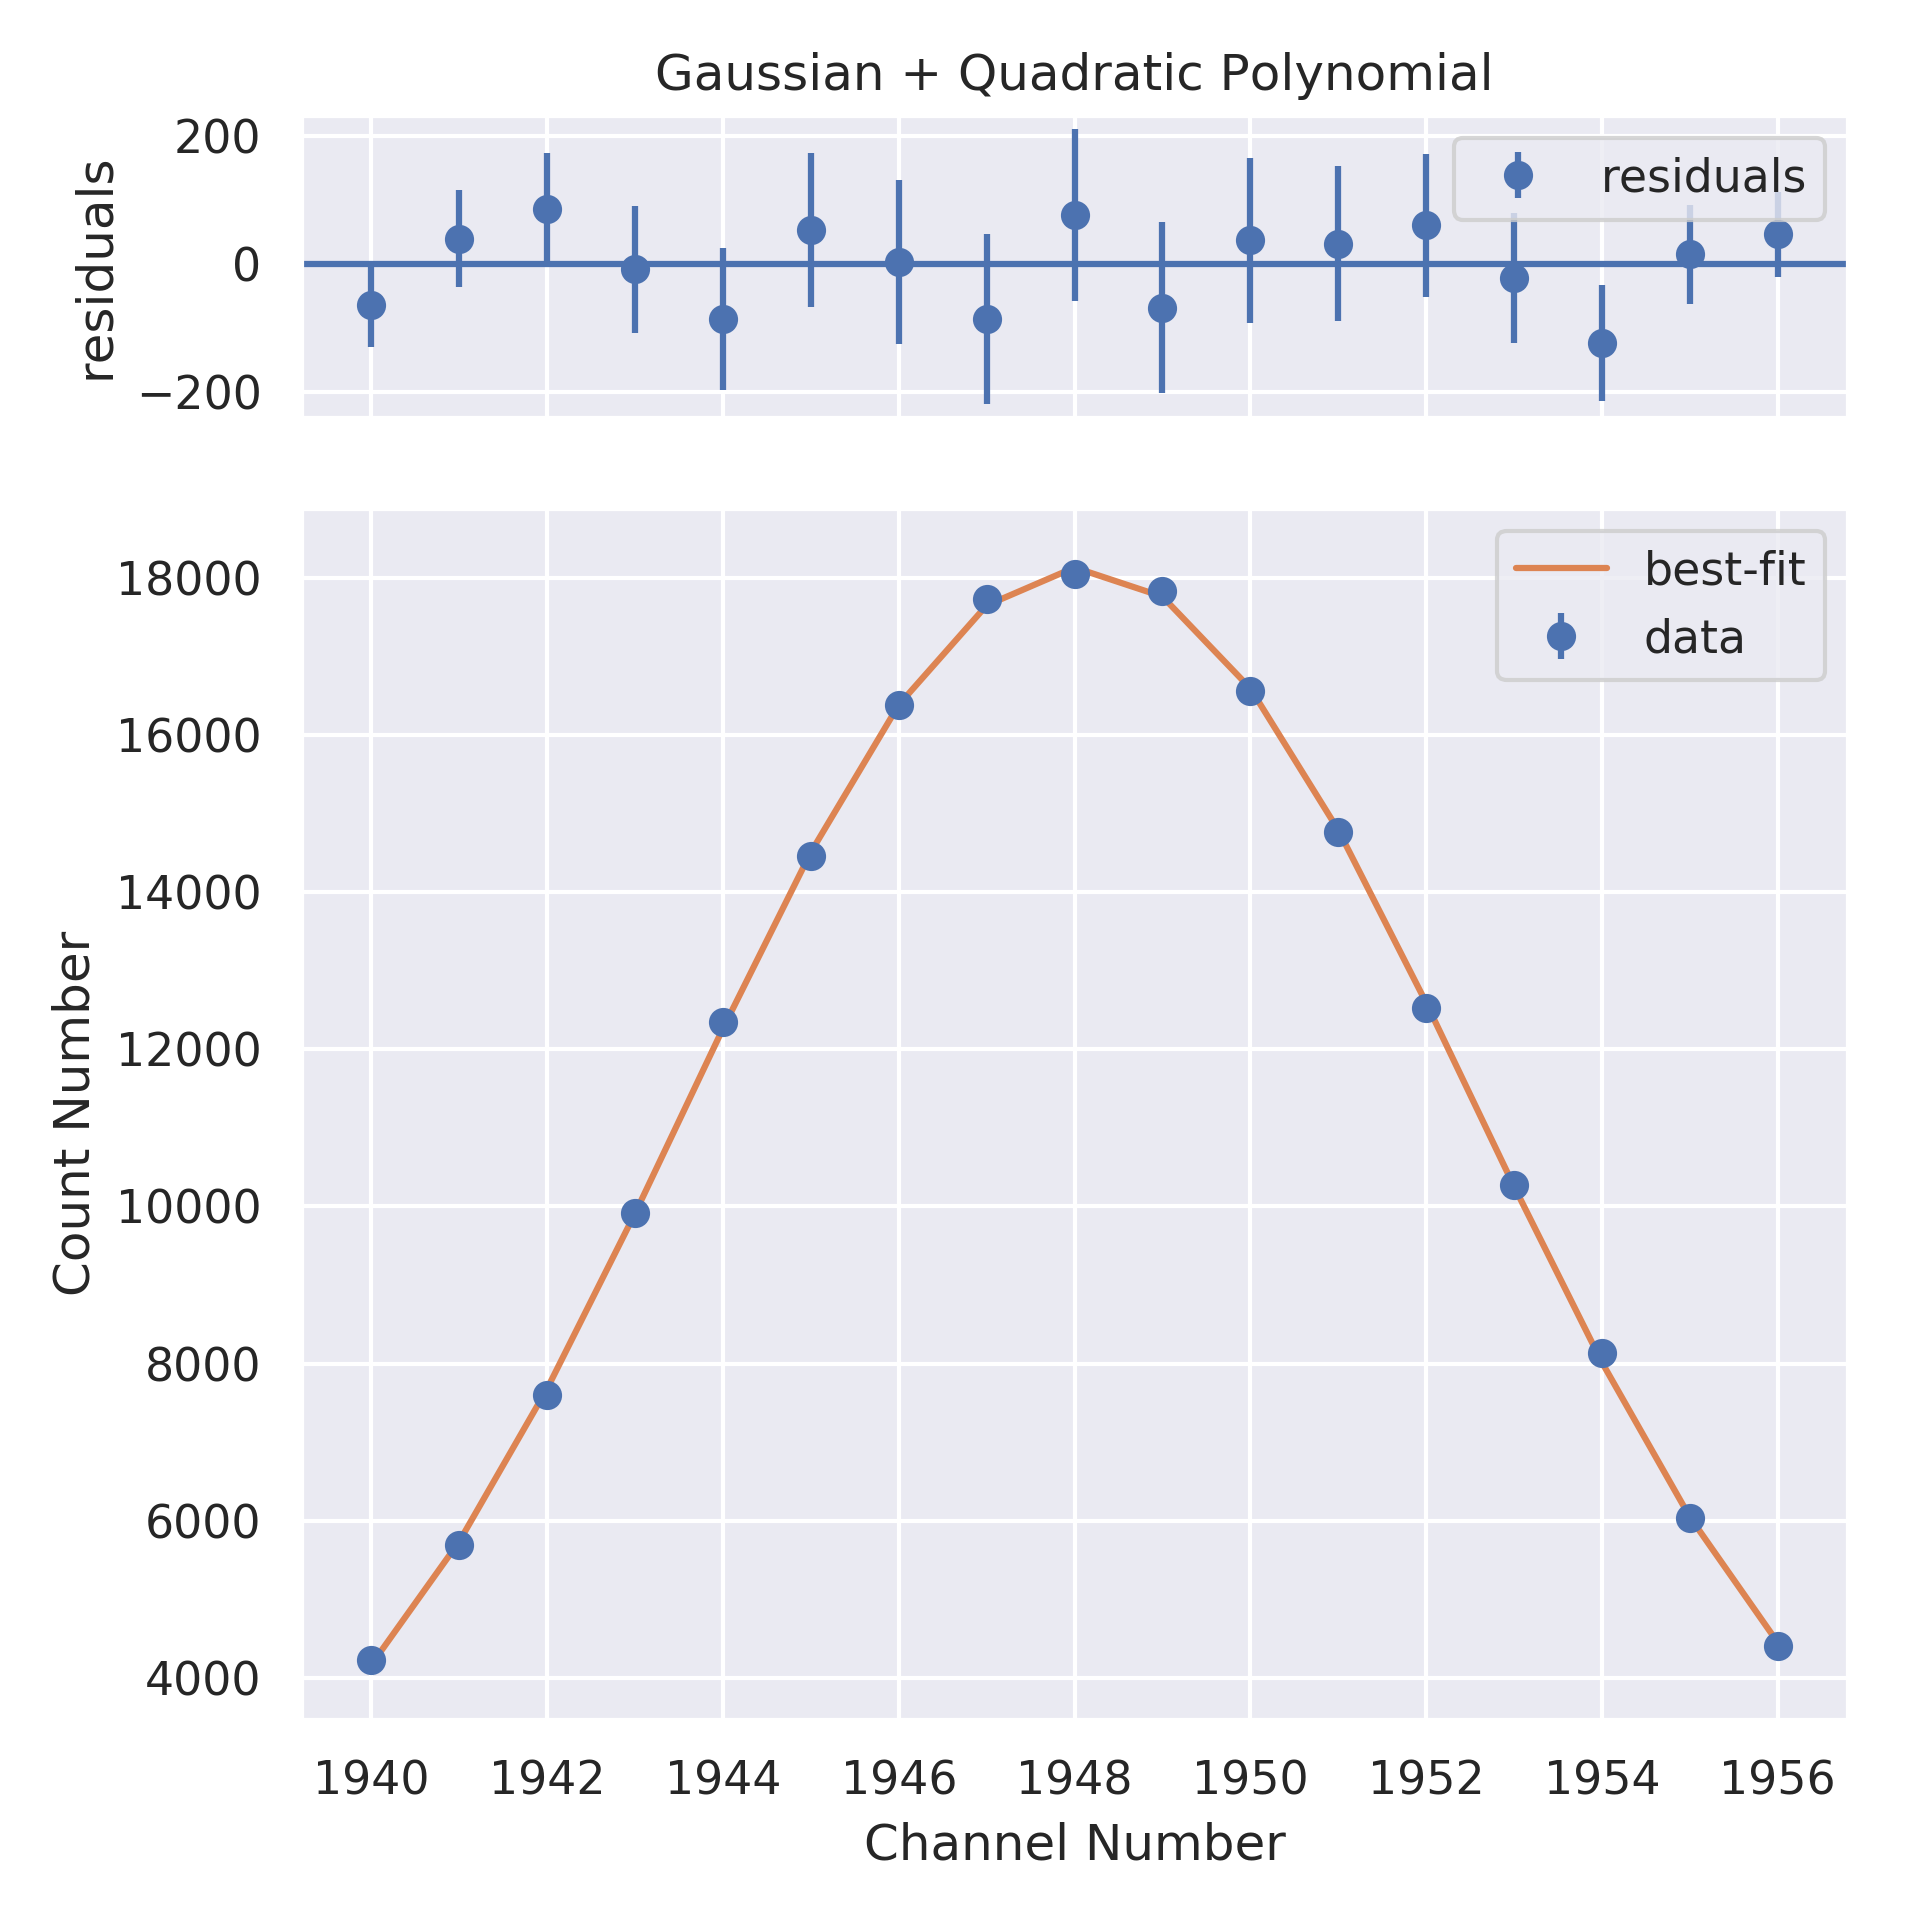
\includegraphics[width=\linewidth]{./Images/Barium133/Quad/Quad_4_Zoom.png}
    \caption{Zoomed in peak with fit. $\chi^2 = 6.91$, $\chi^2_\nu = 0.46$, \\ Prob = 96.00\%, $\mu = 1948.06$, $\sigma = 4.54$}
    %\label{fig:sub2}
  \end{subfigure}
  \caption{Fit of full \& zoomed in peak of \element{Ba}{133} 276 keV peak}
  %\label{fig:test}
\end{figure}
\begin{figure}[H]
  \centering
  \begin{subfigure}{.5\linewidth}
    \centering
    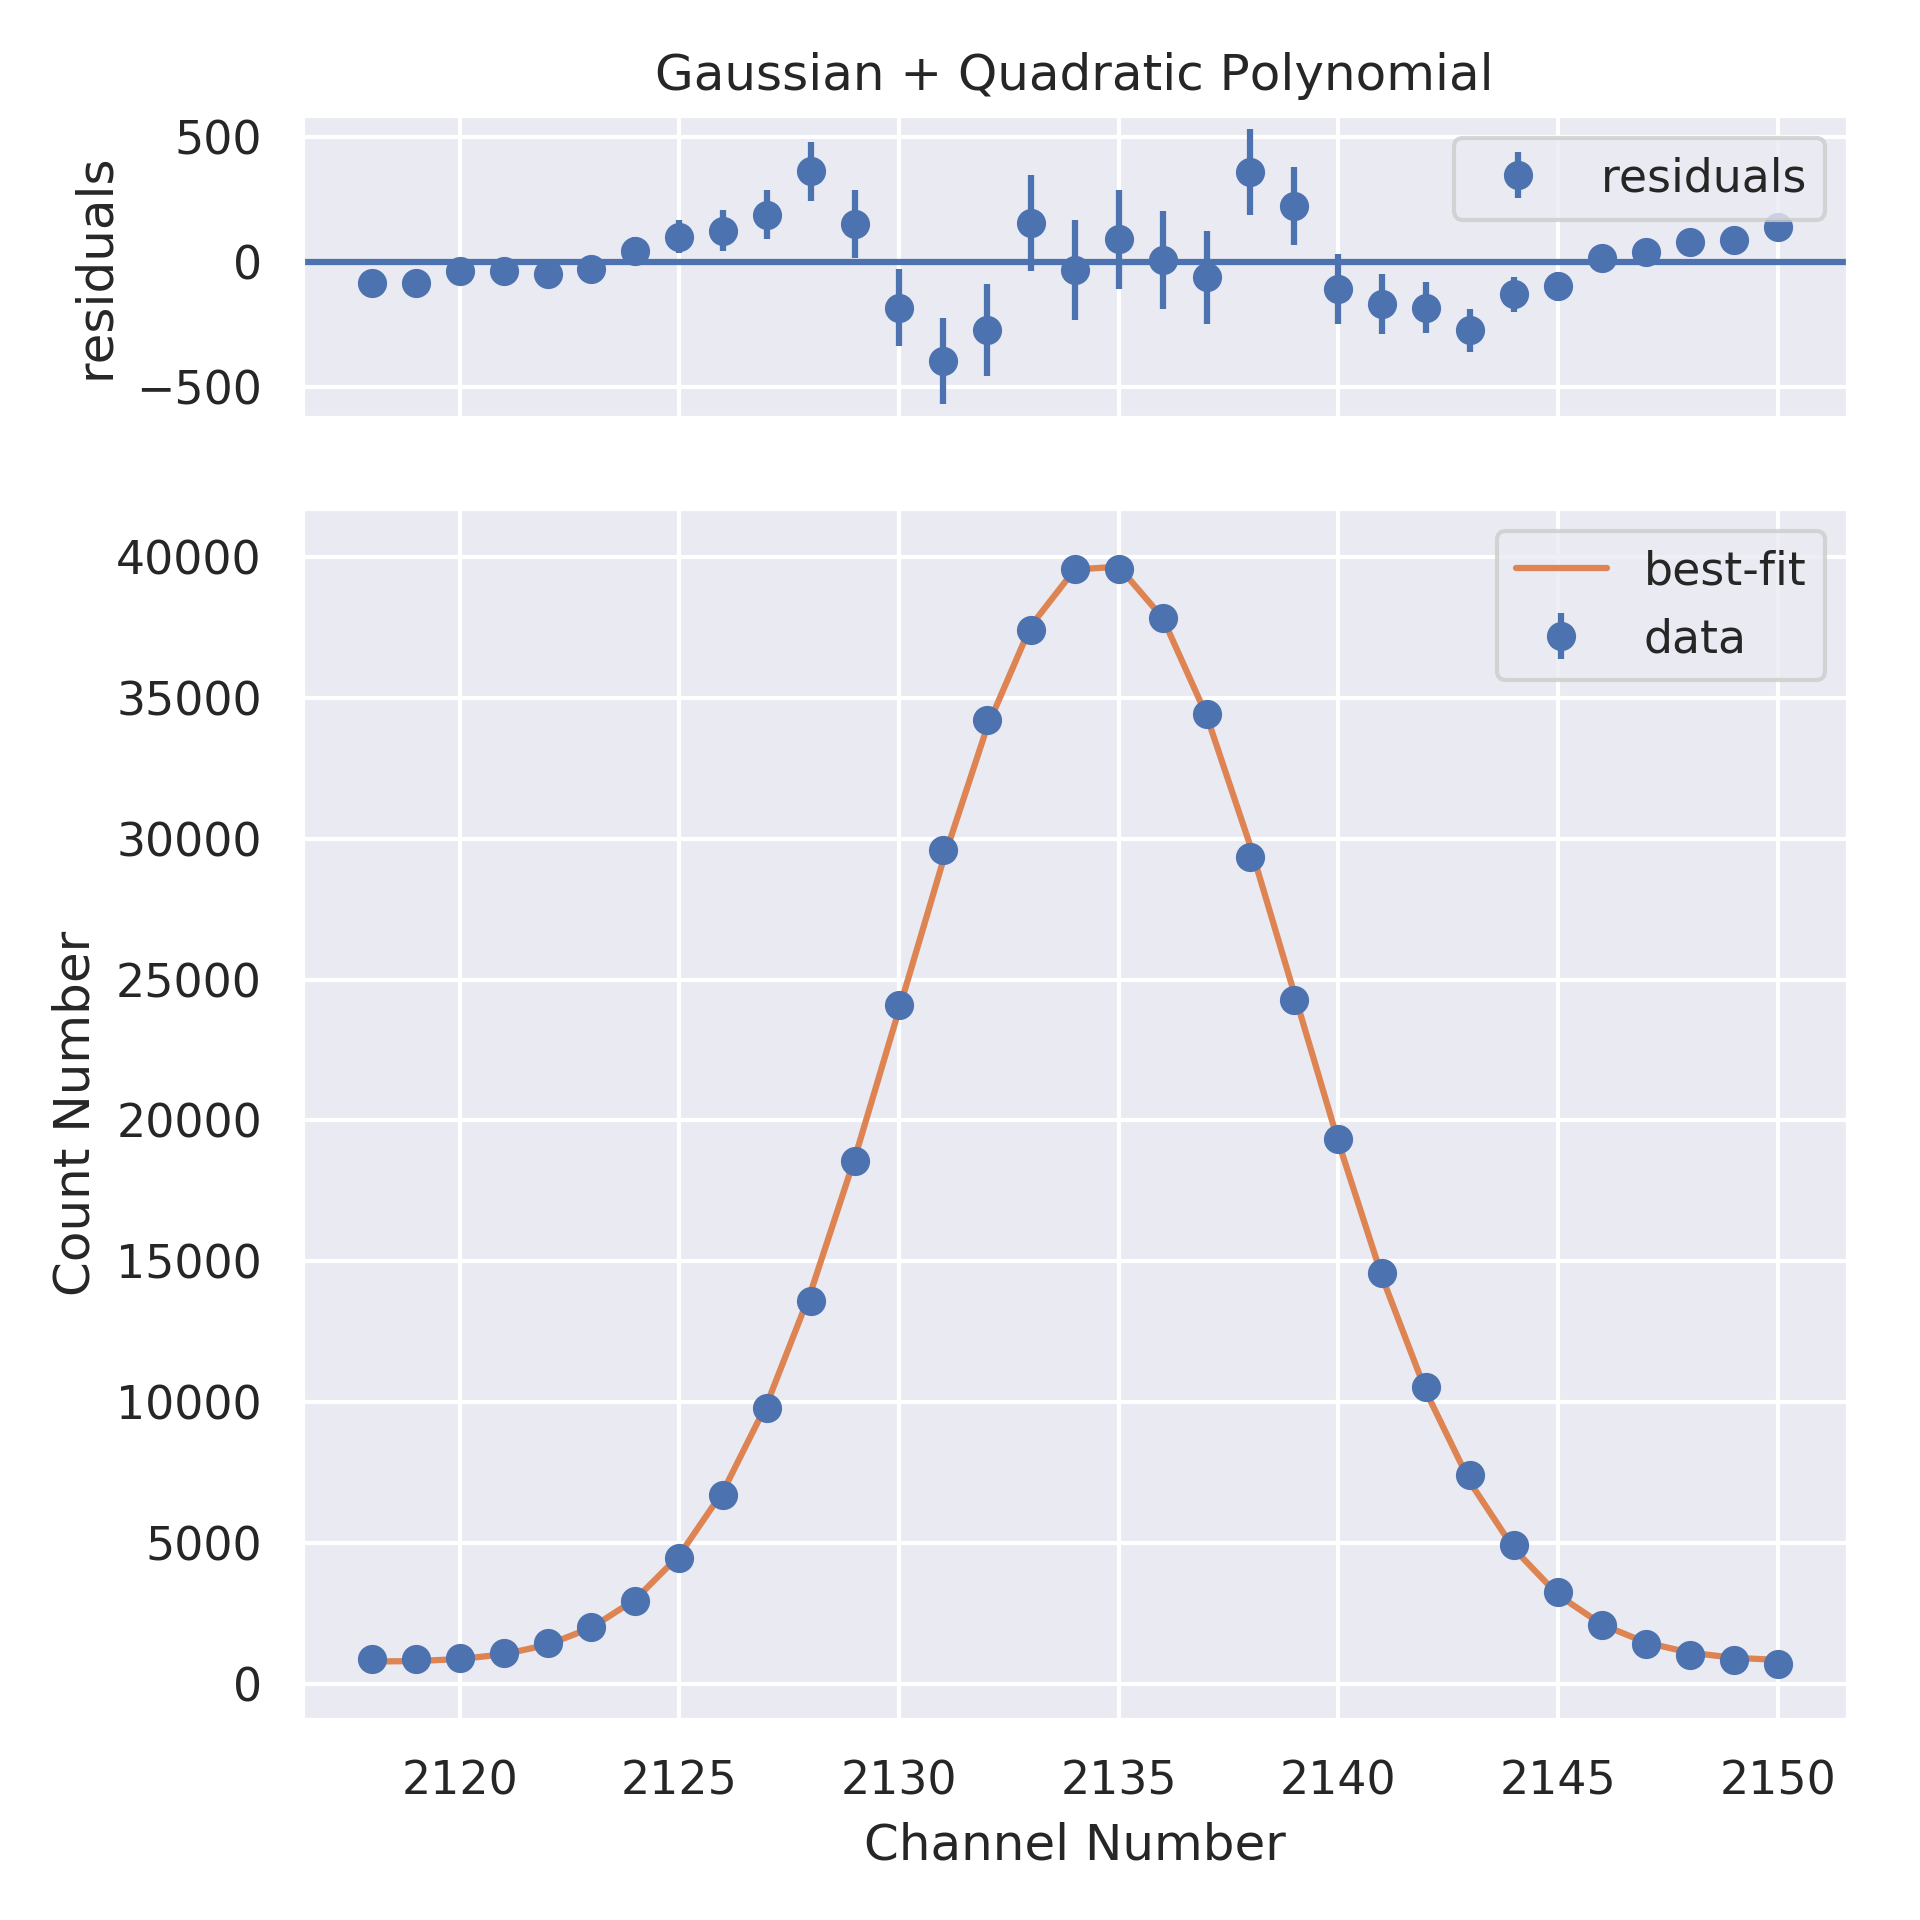
\includegraphics[width=\linewidth]{./Images/Barium133/Quad/Quad_5_Full.png}
    \caption{Full peak with fit $\chi^2 = 123.06$, $\chi^2_\nu = 3.97$, \\ Prob = 0.00\%, $\mu = 2134.55$, $\sigma = 4.47$}
    %\label{fig:sub1}
  \end{subfigure}%
  \begin{subfigure}{.5\linewidth}
    \centering
    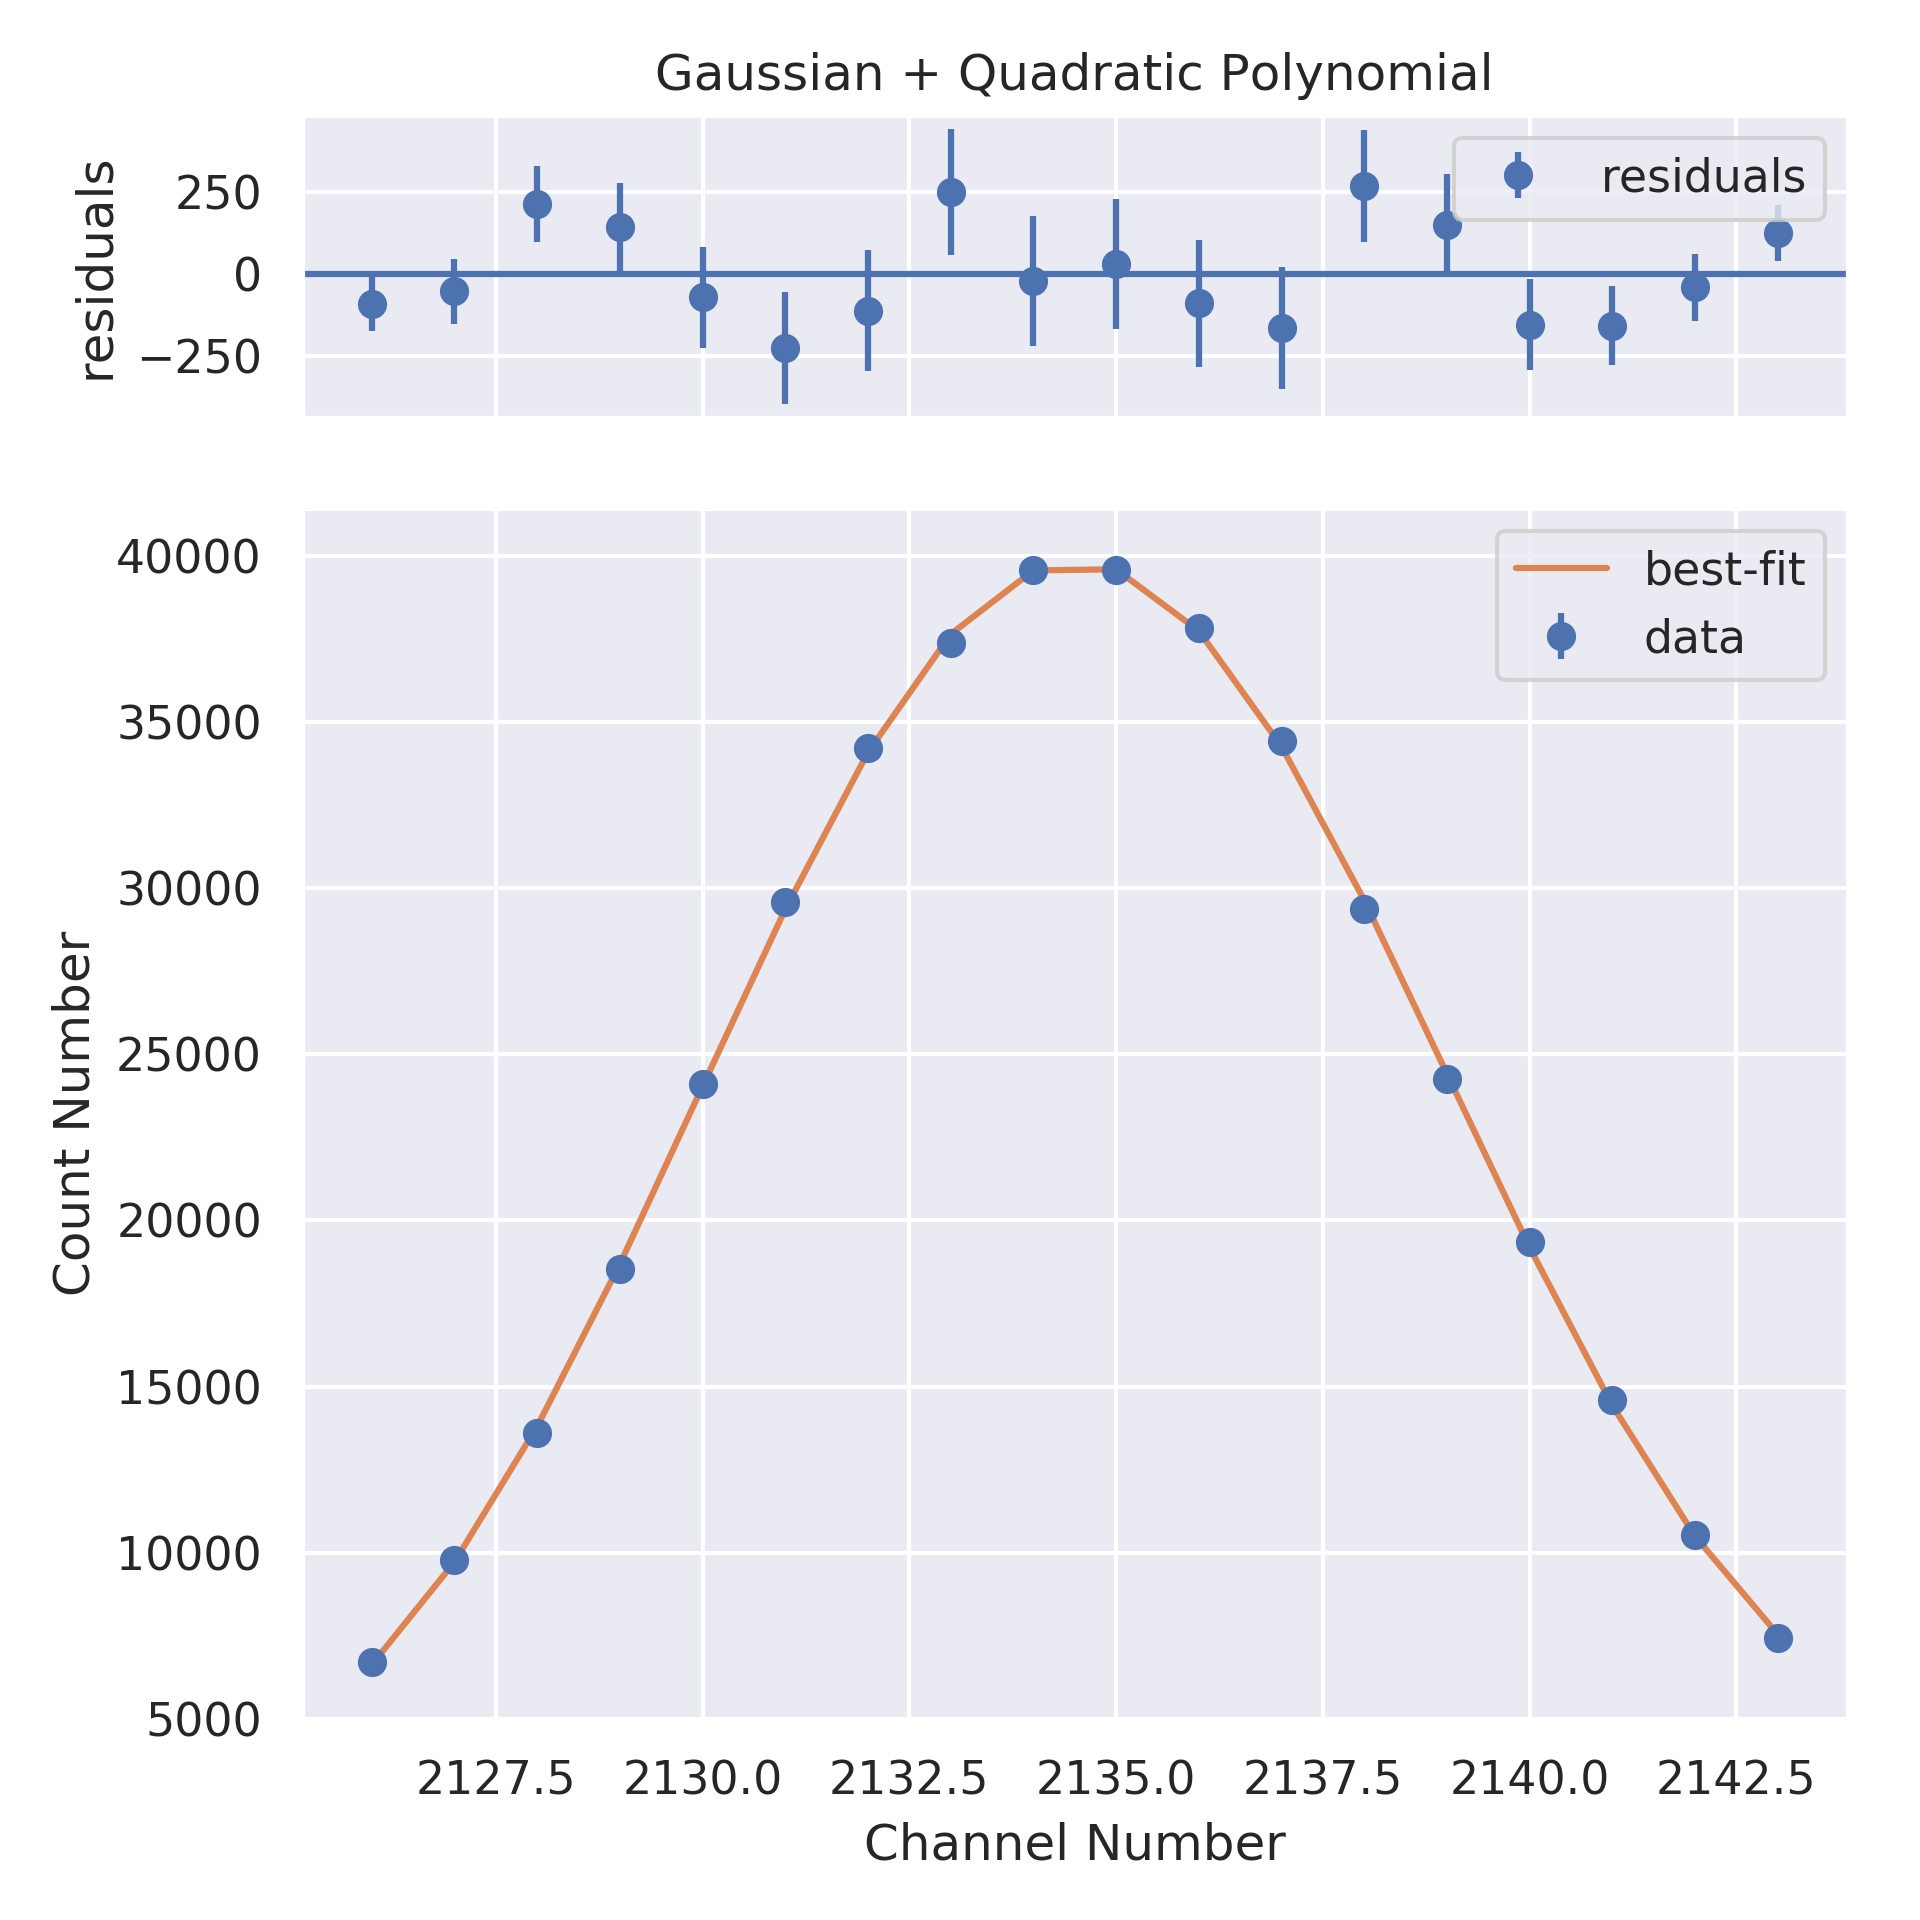
\includegraphics[width=\linewidth]{./Images/Barium133/Quad/Quad_5_Zoom.png}
    \caption{Zoomed in peak with fit. $\chi^2 = 19.63$, $\chi^2_\nu = 1.23$, \\ Prob = 23.74\%, $\mu = 2134.49$, $\sigma = 4.73$}
    %\label{fig:sub2}
  \end{subfigure}
  \caption{Fit of full \& zoomed in peak of \element{Ba}{133} 303 keV peak}
  %\label{fig:test}
\end{figure}
\begin{figure}[H]
  \centering
  \begin{subfigure}{.5\linewidth}
    \centering
    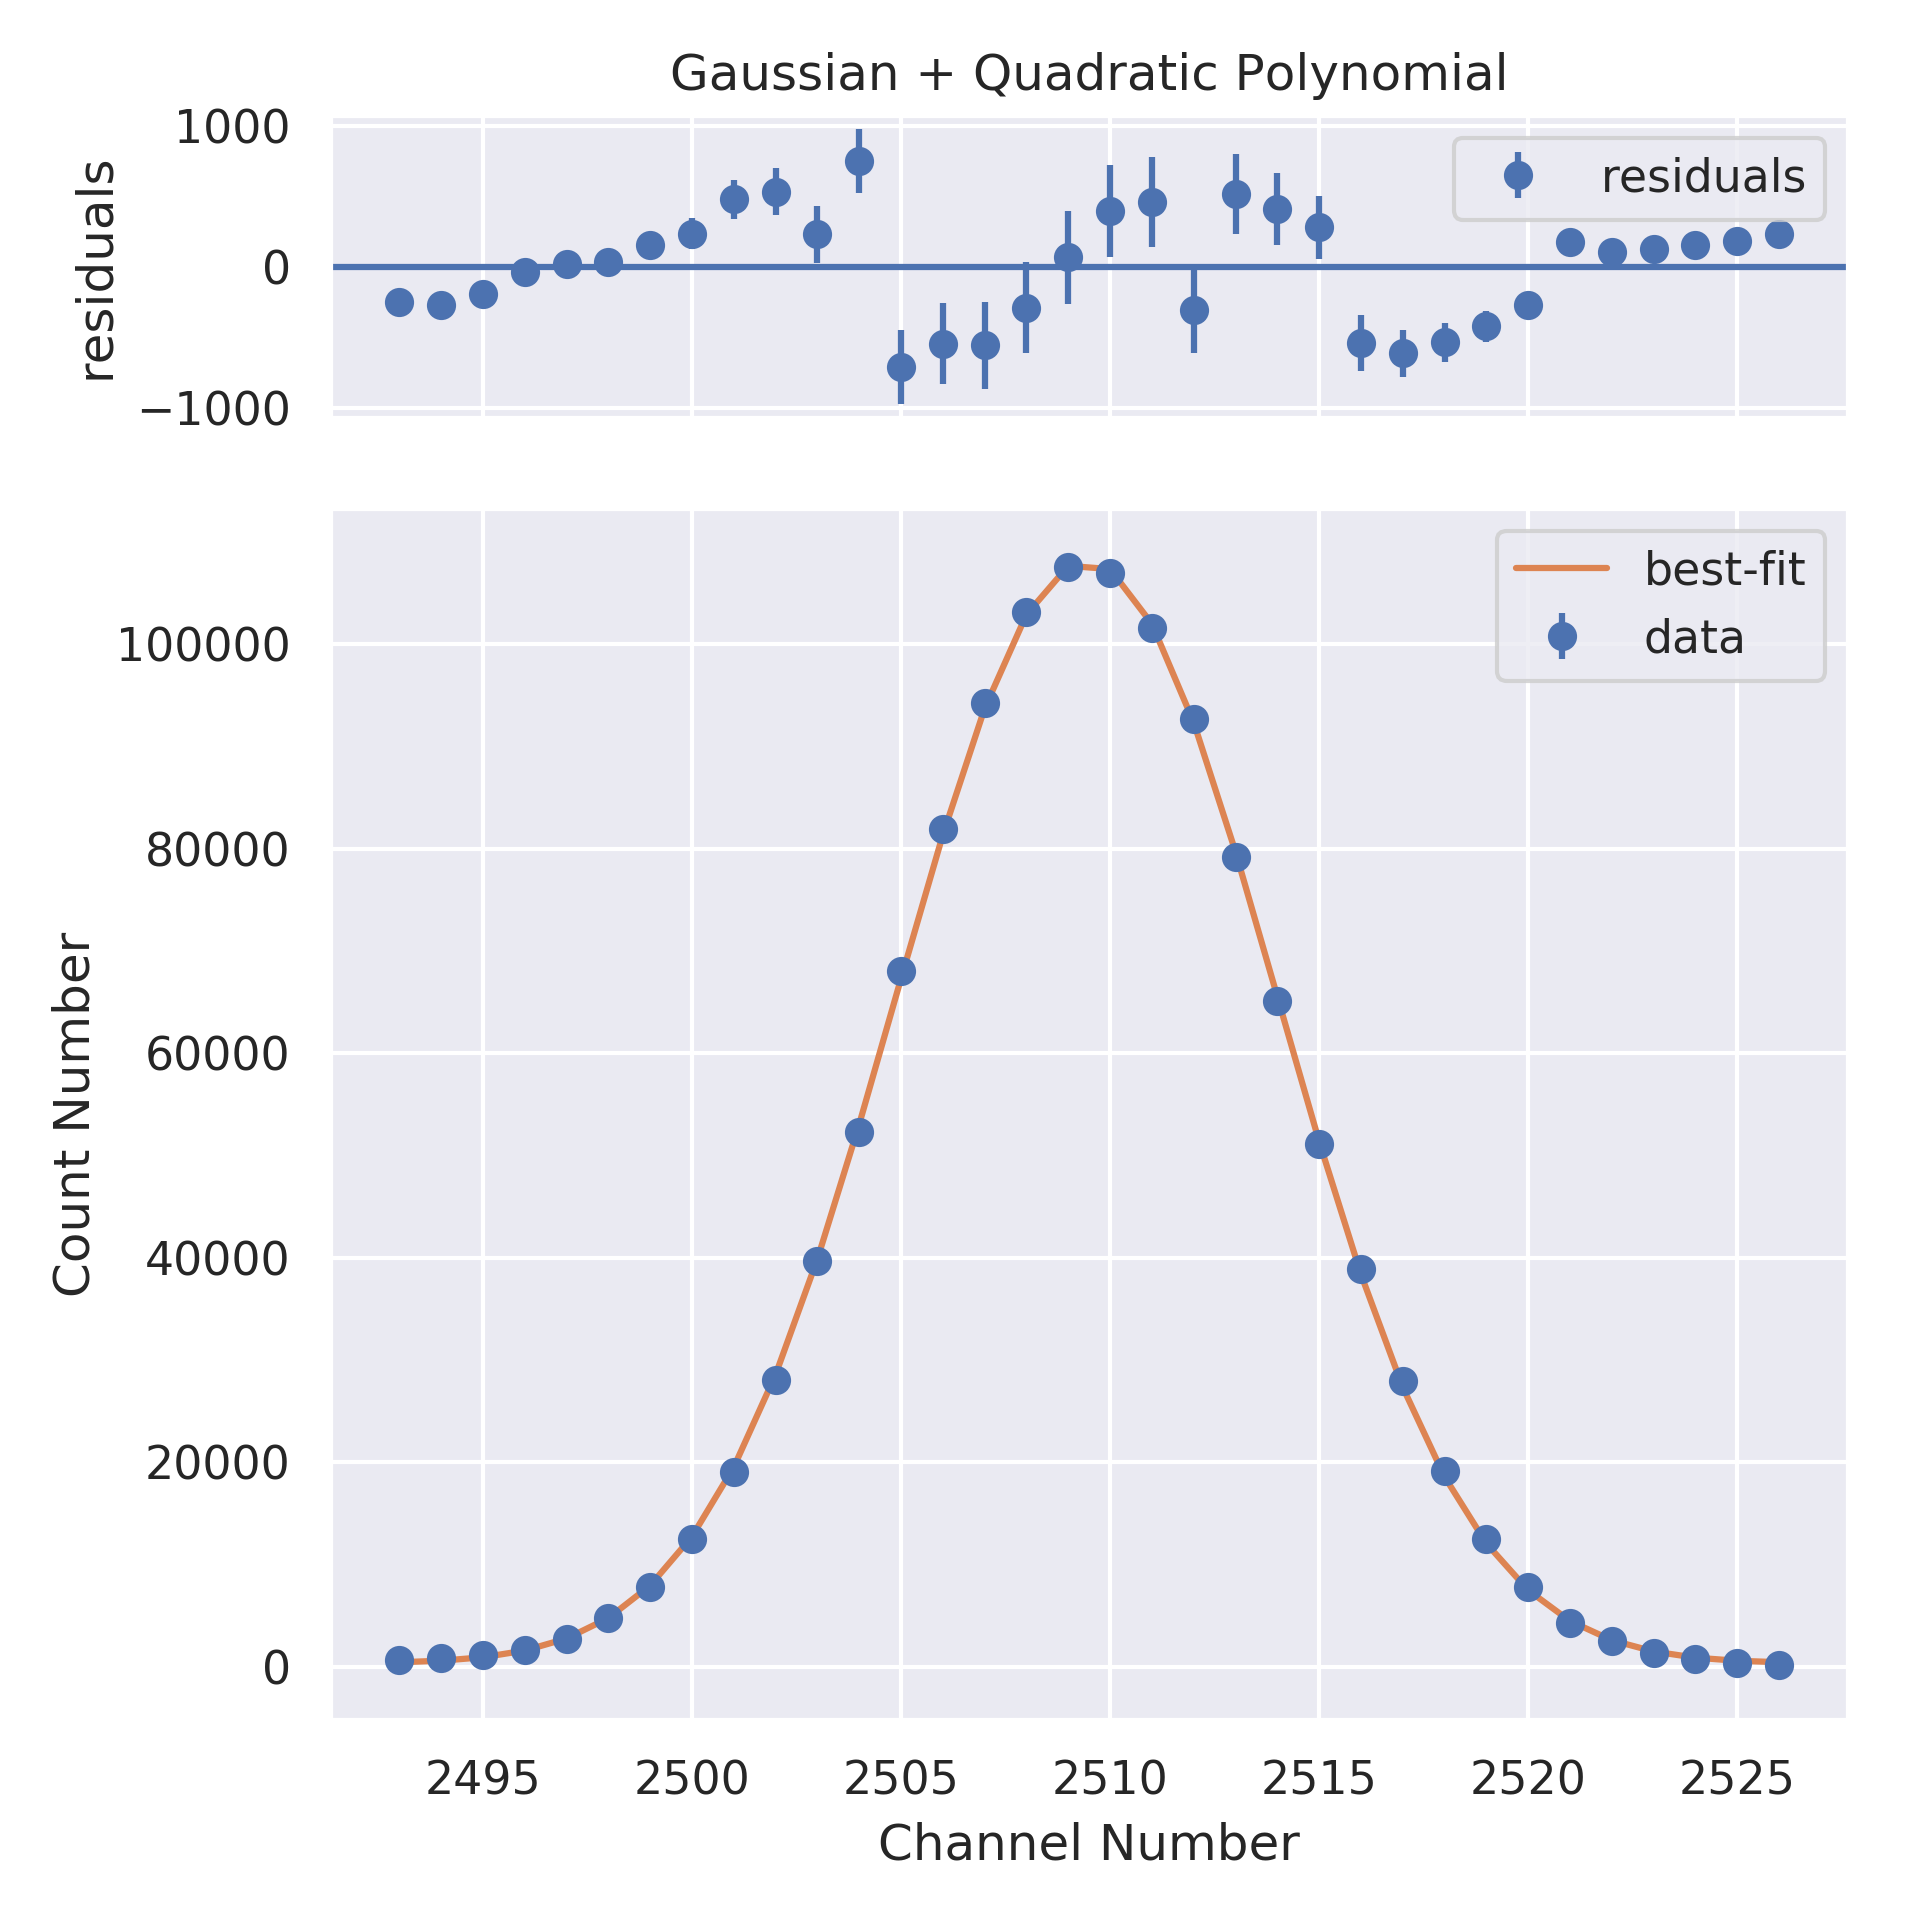
\includegraphics[width=\linewidth]{./Images/Barium133/Quad/Quad_6_Full.png}
    \caption{Full peak with fit. $\chi^2 = 722.64$, $\chi^2_\nu = 22.58$, \\ Prob = 0.00\%, $\mu = 2509.44$, $\sigma = 4.56$}
    %\label{fig:sub1}
  \end{subfigure}%
  \begin{subfigure}{.5\linewidth}
    \centering
    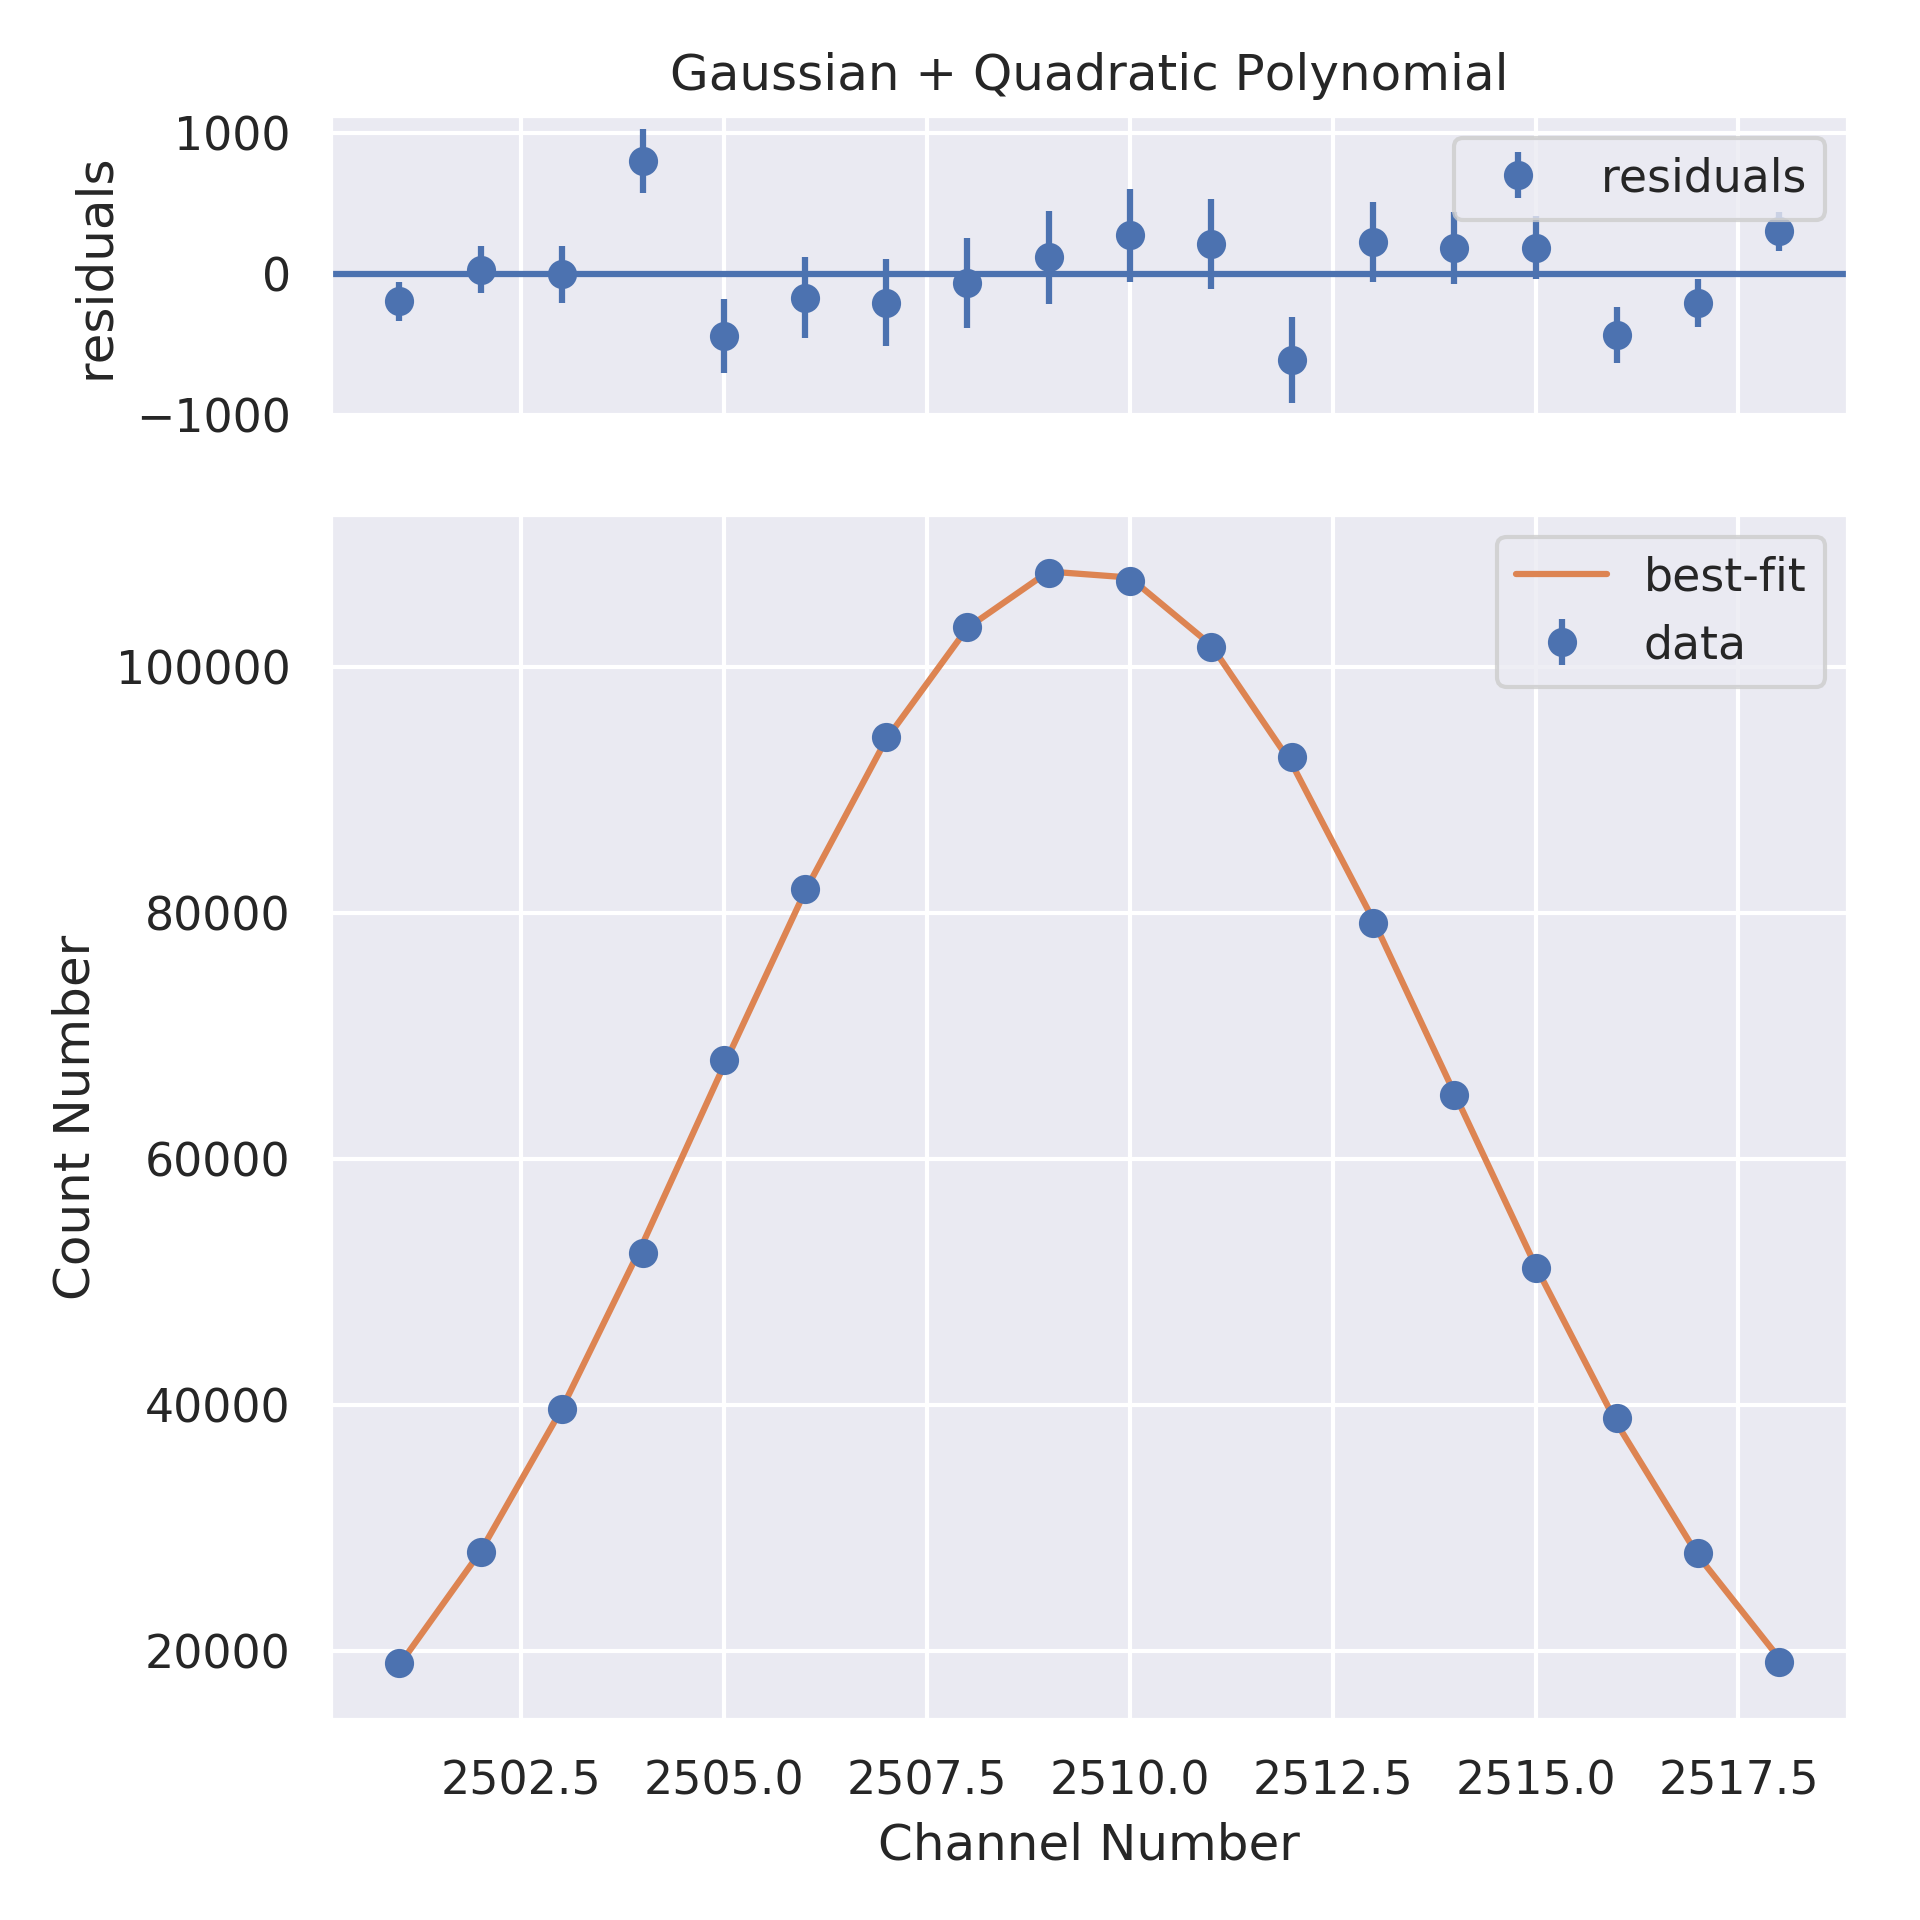
\includegraphics[width=\linewidth]{./Images/Barium133/Quad/Quad_6_Zoom.png}
    \caption{Zoomed in peak with fit. $\chi^2 = 3.14$, $\chi^2_\nu = 2.26$, \\ Prob = 0.28\%, $\mu = 2509.38$, $\sigma = 4.65$}
    %\label{fig:sub2}
  \end{subfigure}
  \caption{Fit of full \& zoomed in peak of \element{Ba}{133} 356 keV peak}
  %\label{fig:test}
\end{figure}
\begin{figure}[H]
  \centering
  \begin{subfigure}{.5\linewidth}
    \centering
    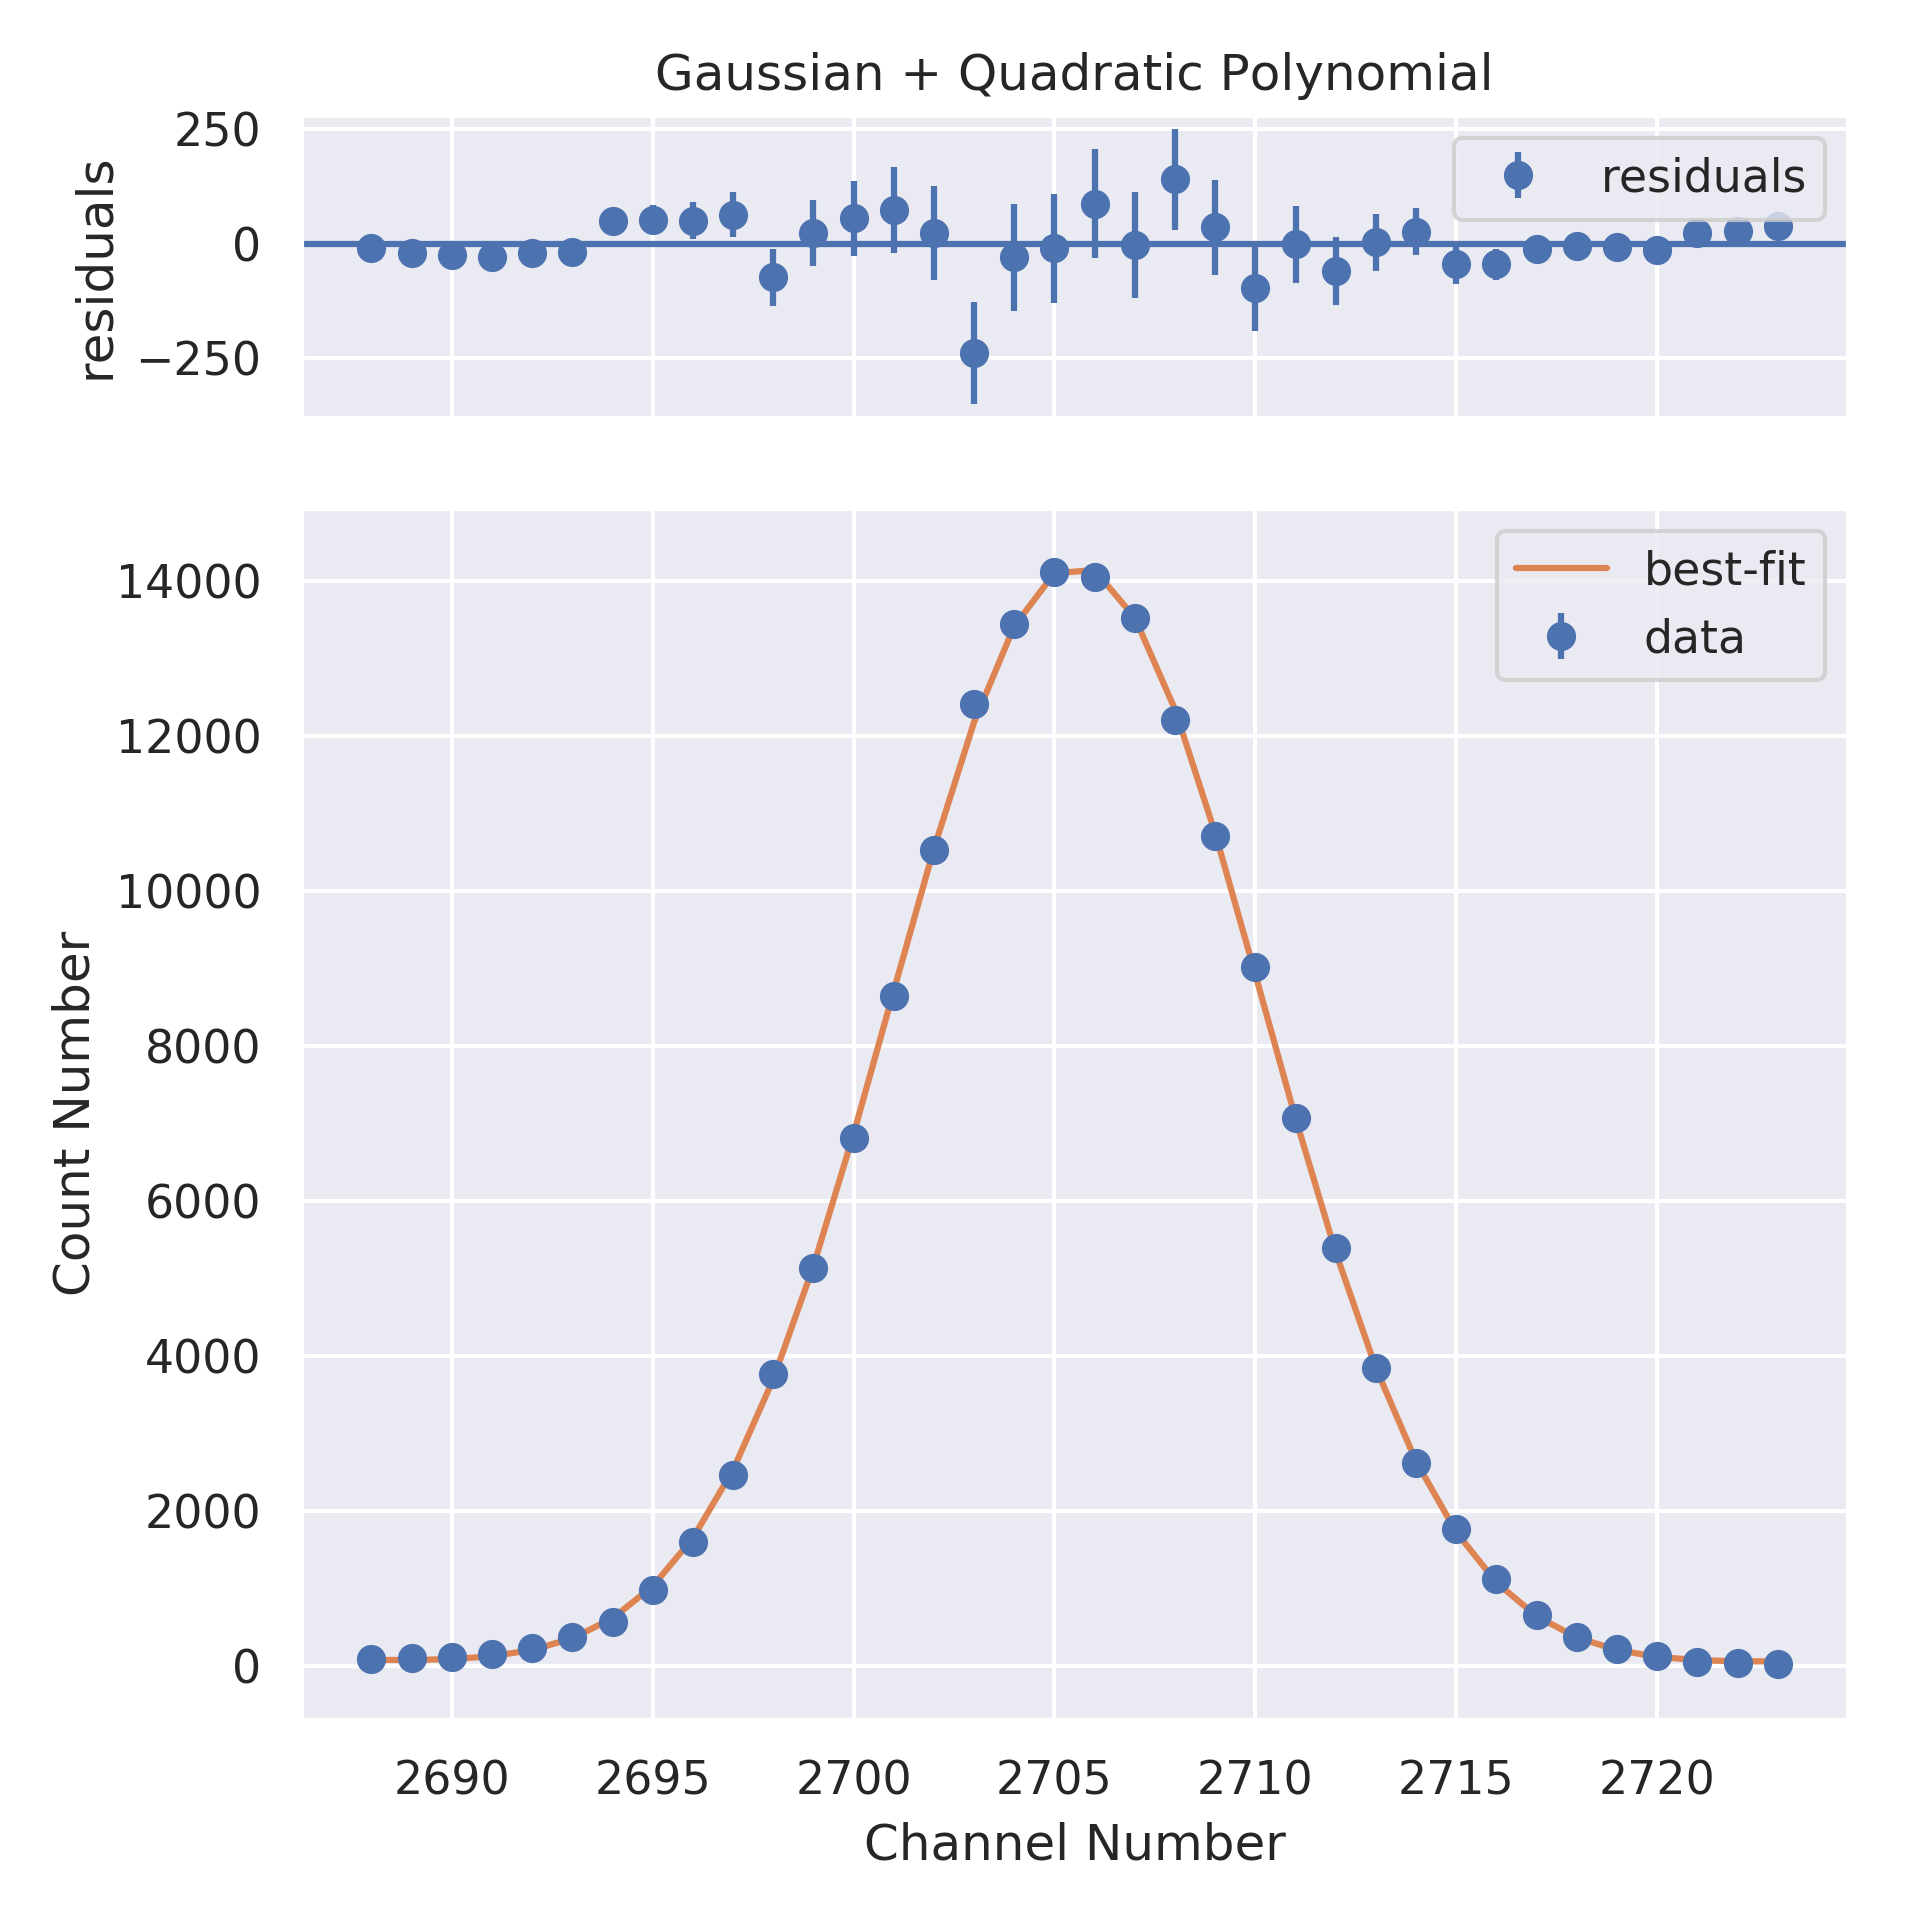
\includegraphics[width=\linewidth]{./Images/Barium133/Quad/Quad_7_Full.png}
    \caption{Full peak with fit. $\chi^2 = 119.72$, $\chi^2_\nu = 3.52$, \\ Prob = 0.00\%, $\mu = 2705.56$, $\sigma = 4.62$}
    %\label{fig:sub1}
  \end{subfigure}%
  \begin{subfigure}{.5\linewidth}
    \centering
    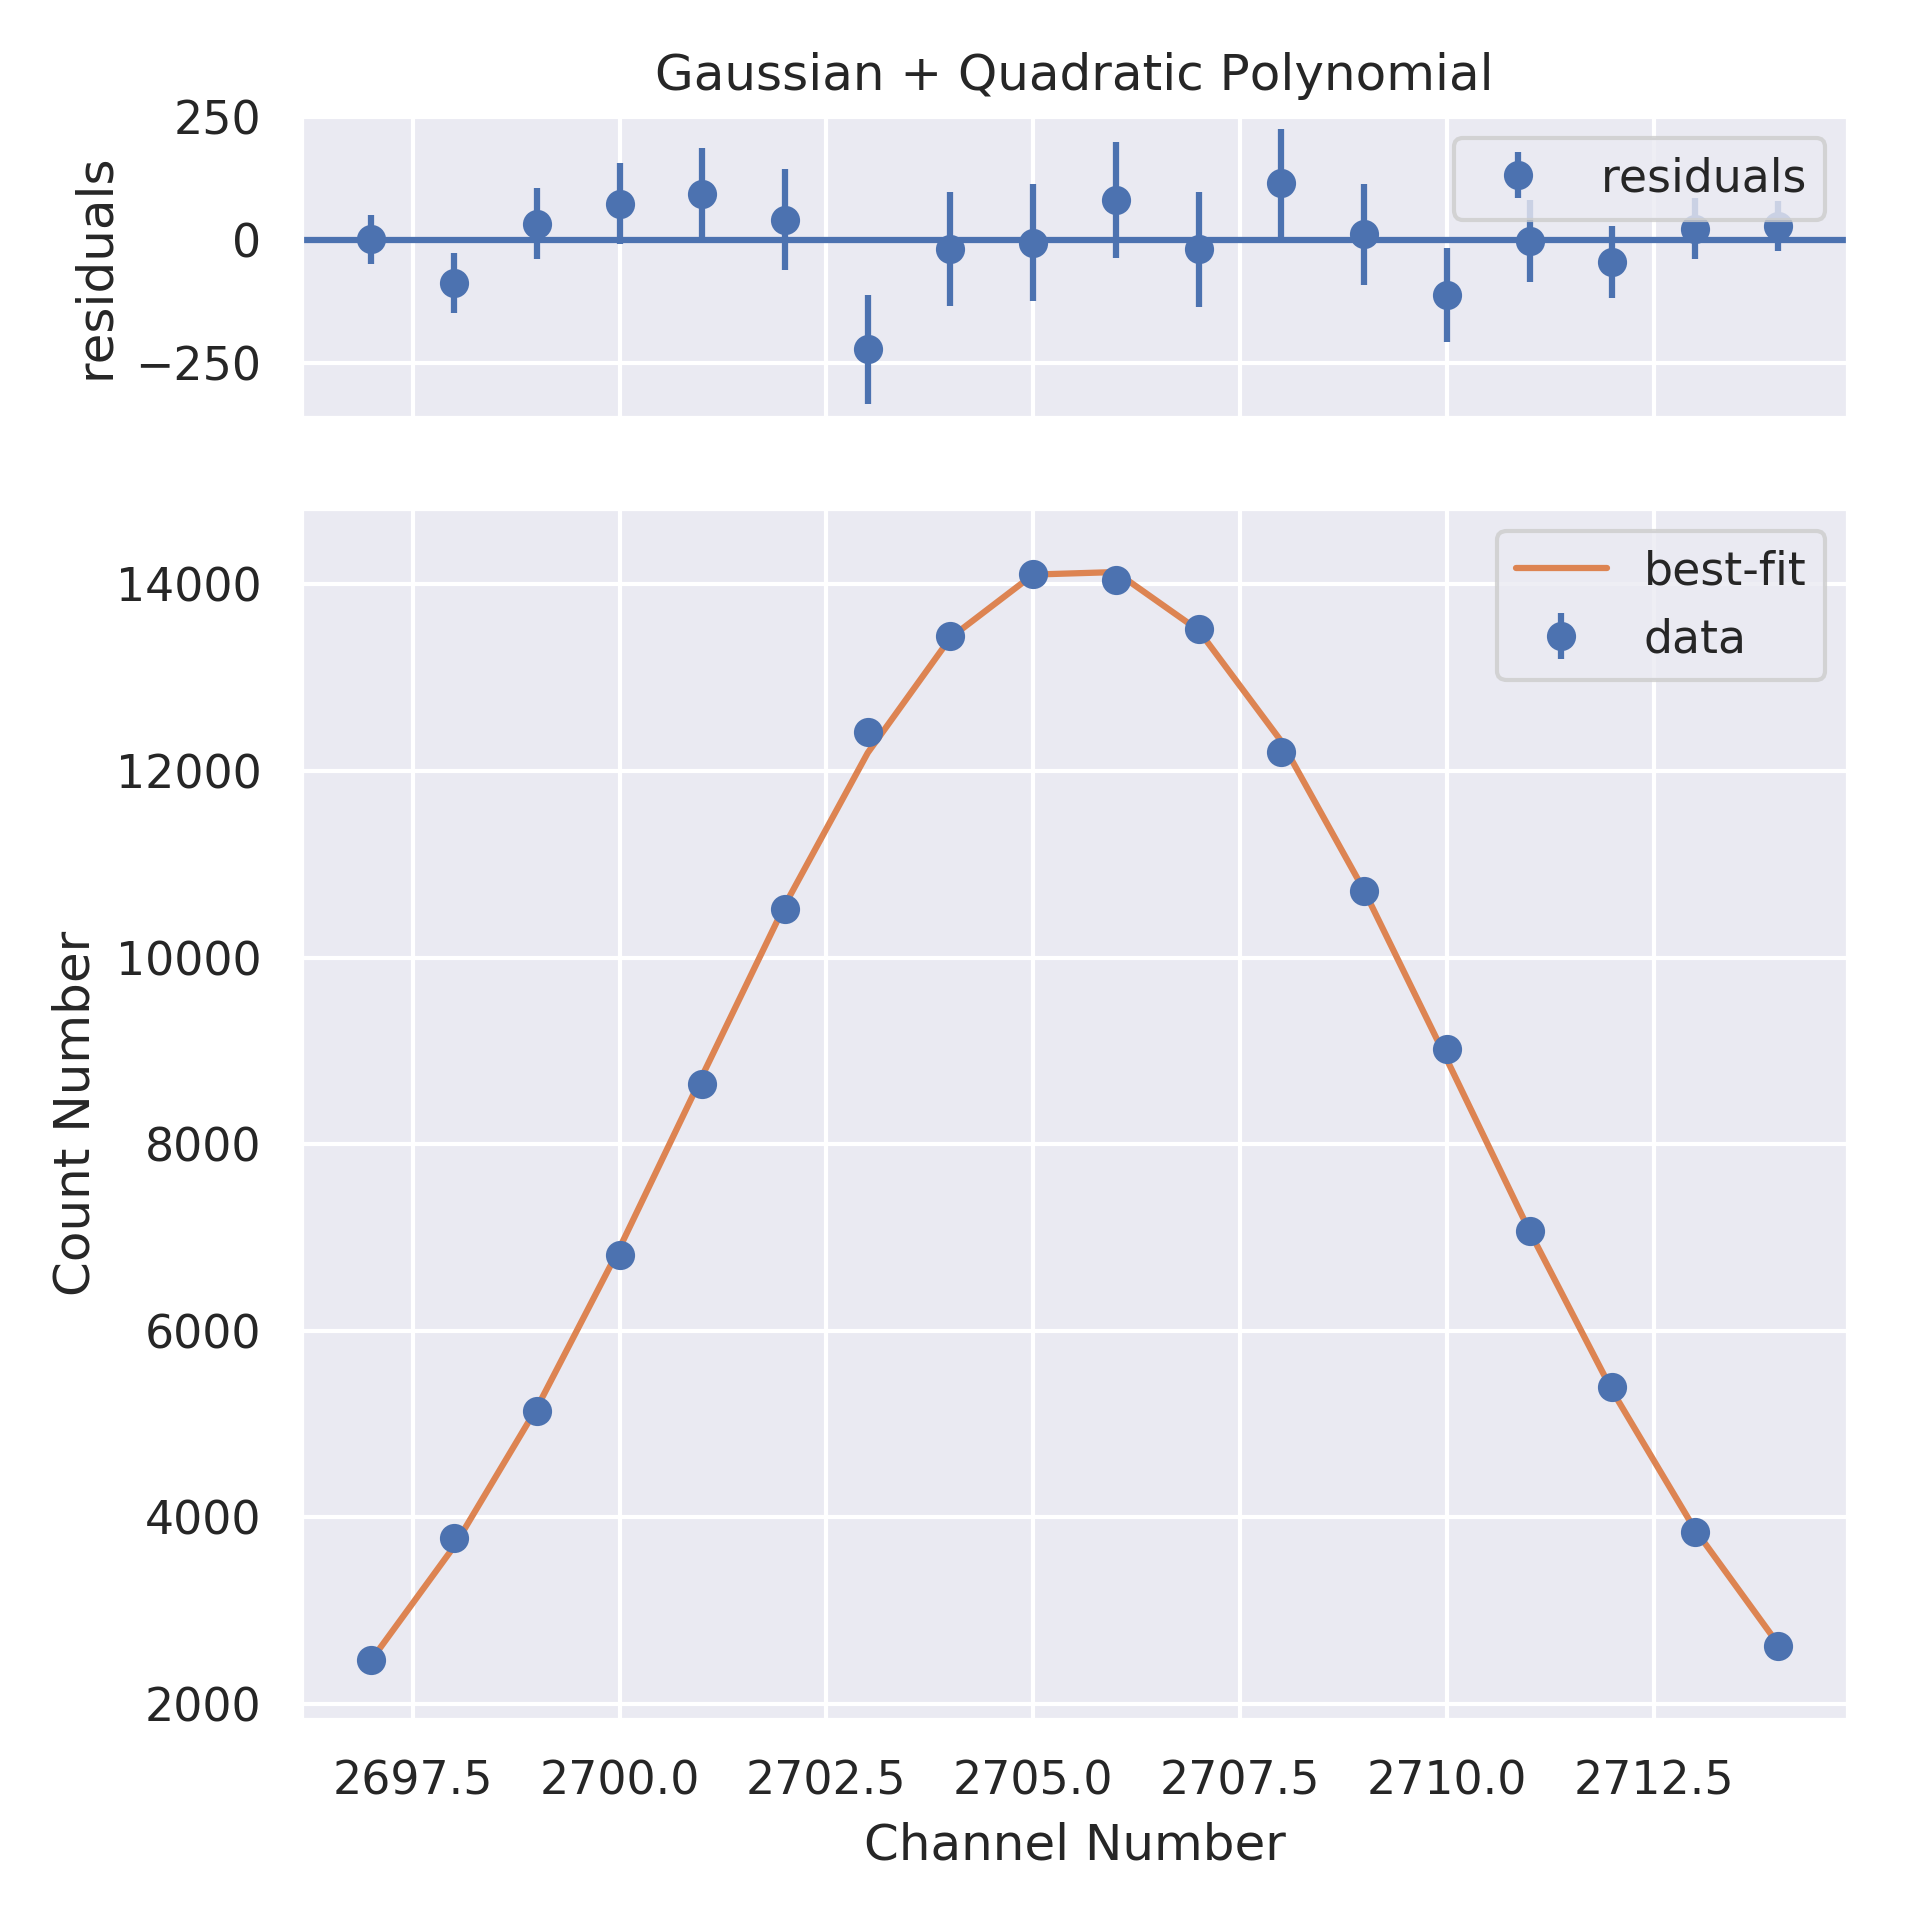
\includegraphics[width=\linewidth]{./Images/Barium133/Quad/Quad_7_Zoom.png}
    \caption{Zoomed in peak with fit. $\chi^2 = 12.07$, $\chi^2_\nu = 0.75$, \\ Prob = 73.93\%, $\mu = 2705.53$, $\sigma = 4.50$}
    %\label{fig:sub2}
  \end{subfigure}
  \caption{Fit of full \& zoomed in peak of \element{Ba}{133} 384 keV peak}
  %\label{fig:test}
\end{figure}
\clearpage

\subsection{Cobalt-60}
The \element{Co}{60} source had two high-energy peaks which were very distinctive, and so quite easy to fit for all functions.
\begin{figure}[H]
  \centering
  \includegraphics[width=0.95\linewidth]{./Images/Cobalt60/Final_Cobalt24hr.png}
  \caption{The final spectrum obtained for the \element{Co}{60} source run for 24 hours. This has been converted to energies by using the quadratic energy calibration.}
\end{figure} 
\subsubsection{Gaussian + Offset Fit}
\begin{figure}[H]
  \centering
  \begin{subfigure}{.5\linewidth}
    \centering
    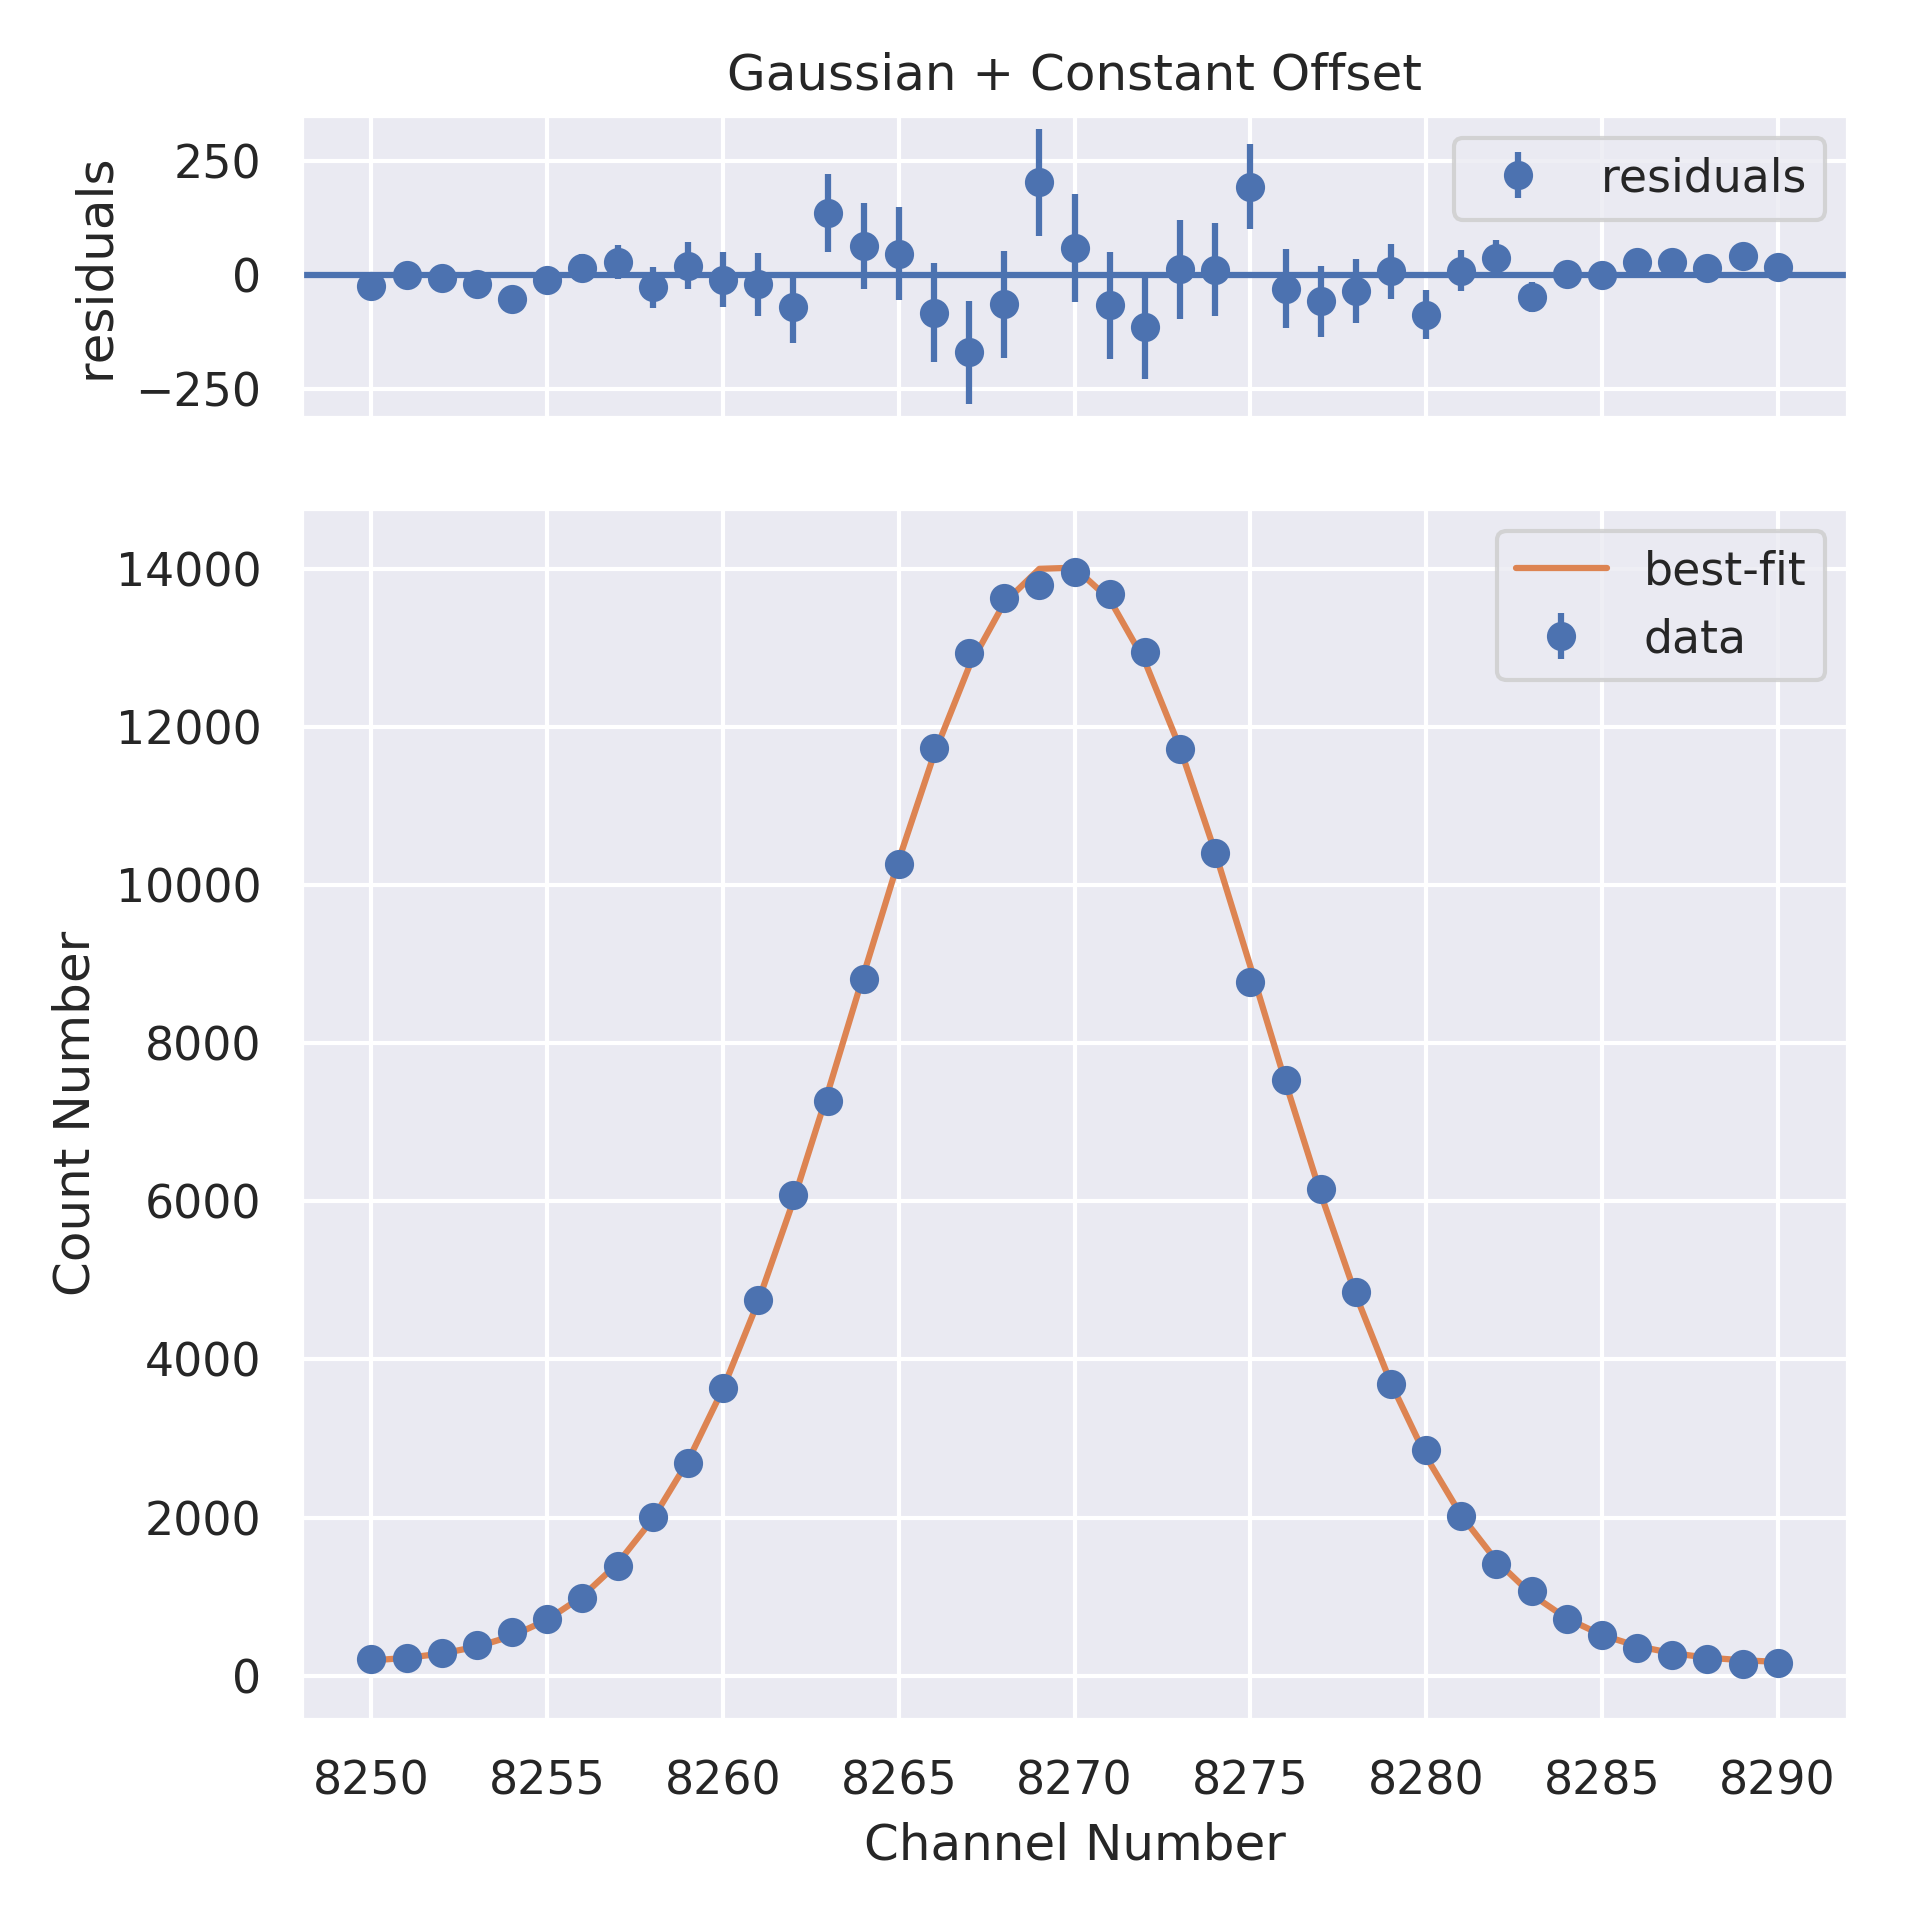
\includegraphics[width=\linewidth]{./Images/Cobalt60/Gauss/Gauss_1_Full.png}
    \caption{Full peak with fit. $\chi^2 = 54.04$, $\chi^2_\nu = 1.39$, \\ Prob = 5.52\%, $\mu = 8269.53$, $\sigma = 5.73$}
    %\label{fig:sub1}
  \end{subfigure}%
  \begin{subfigure}{.5\linewidth}
    \centering
    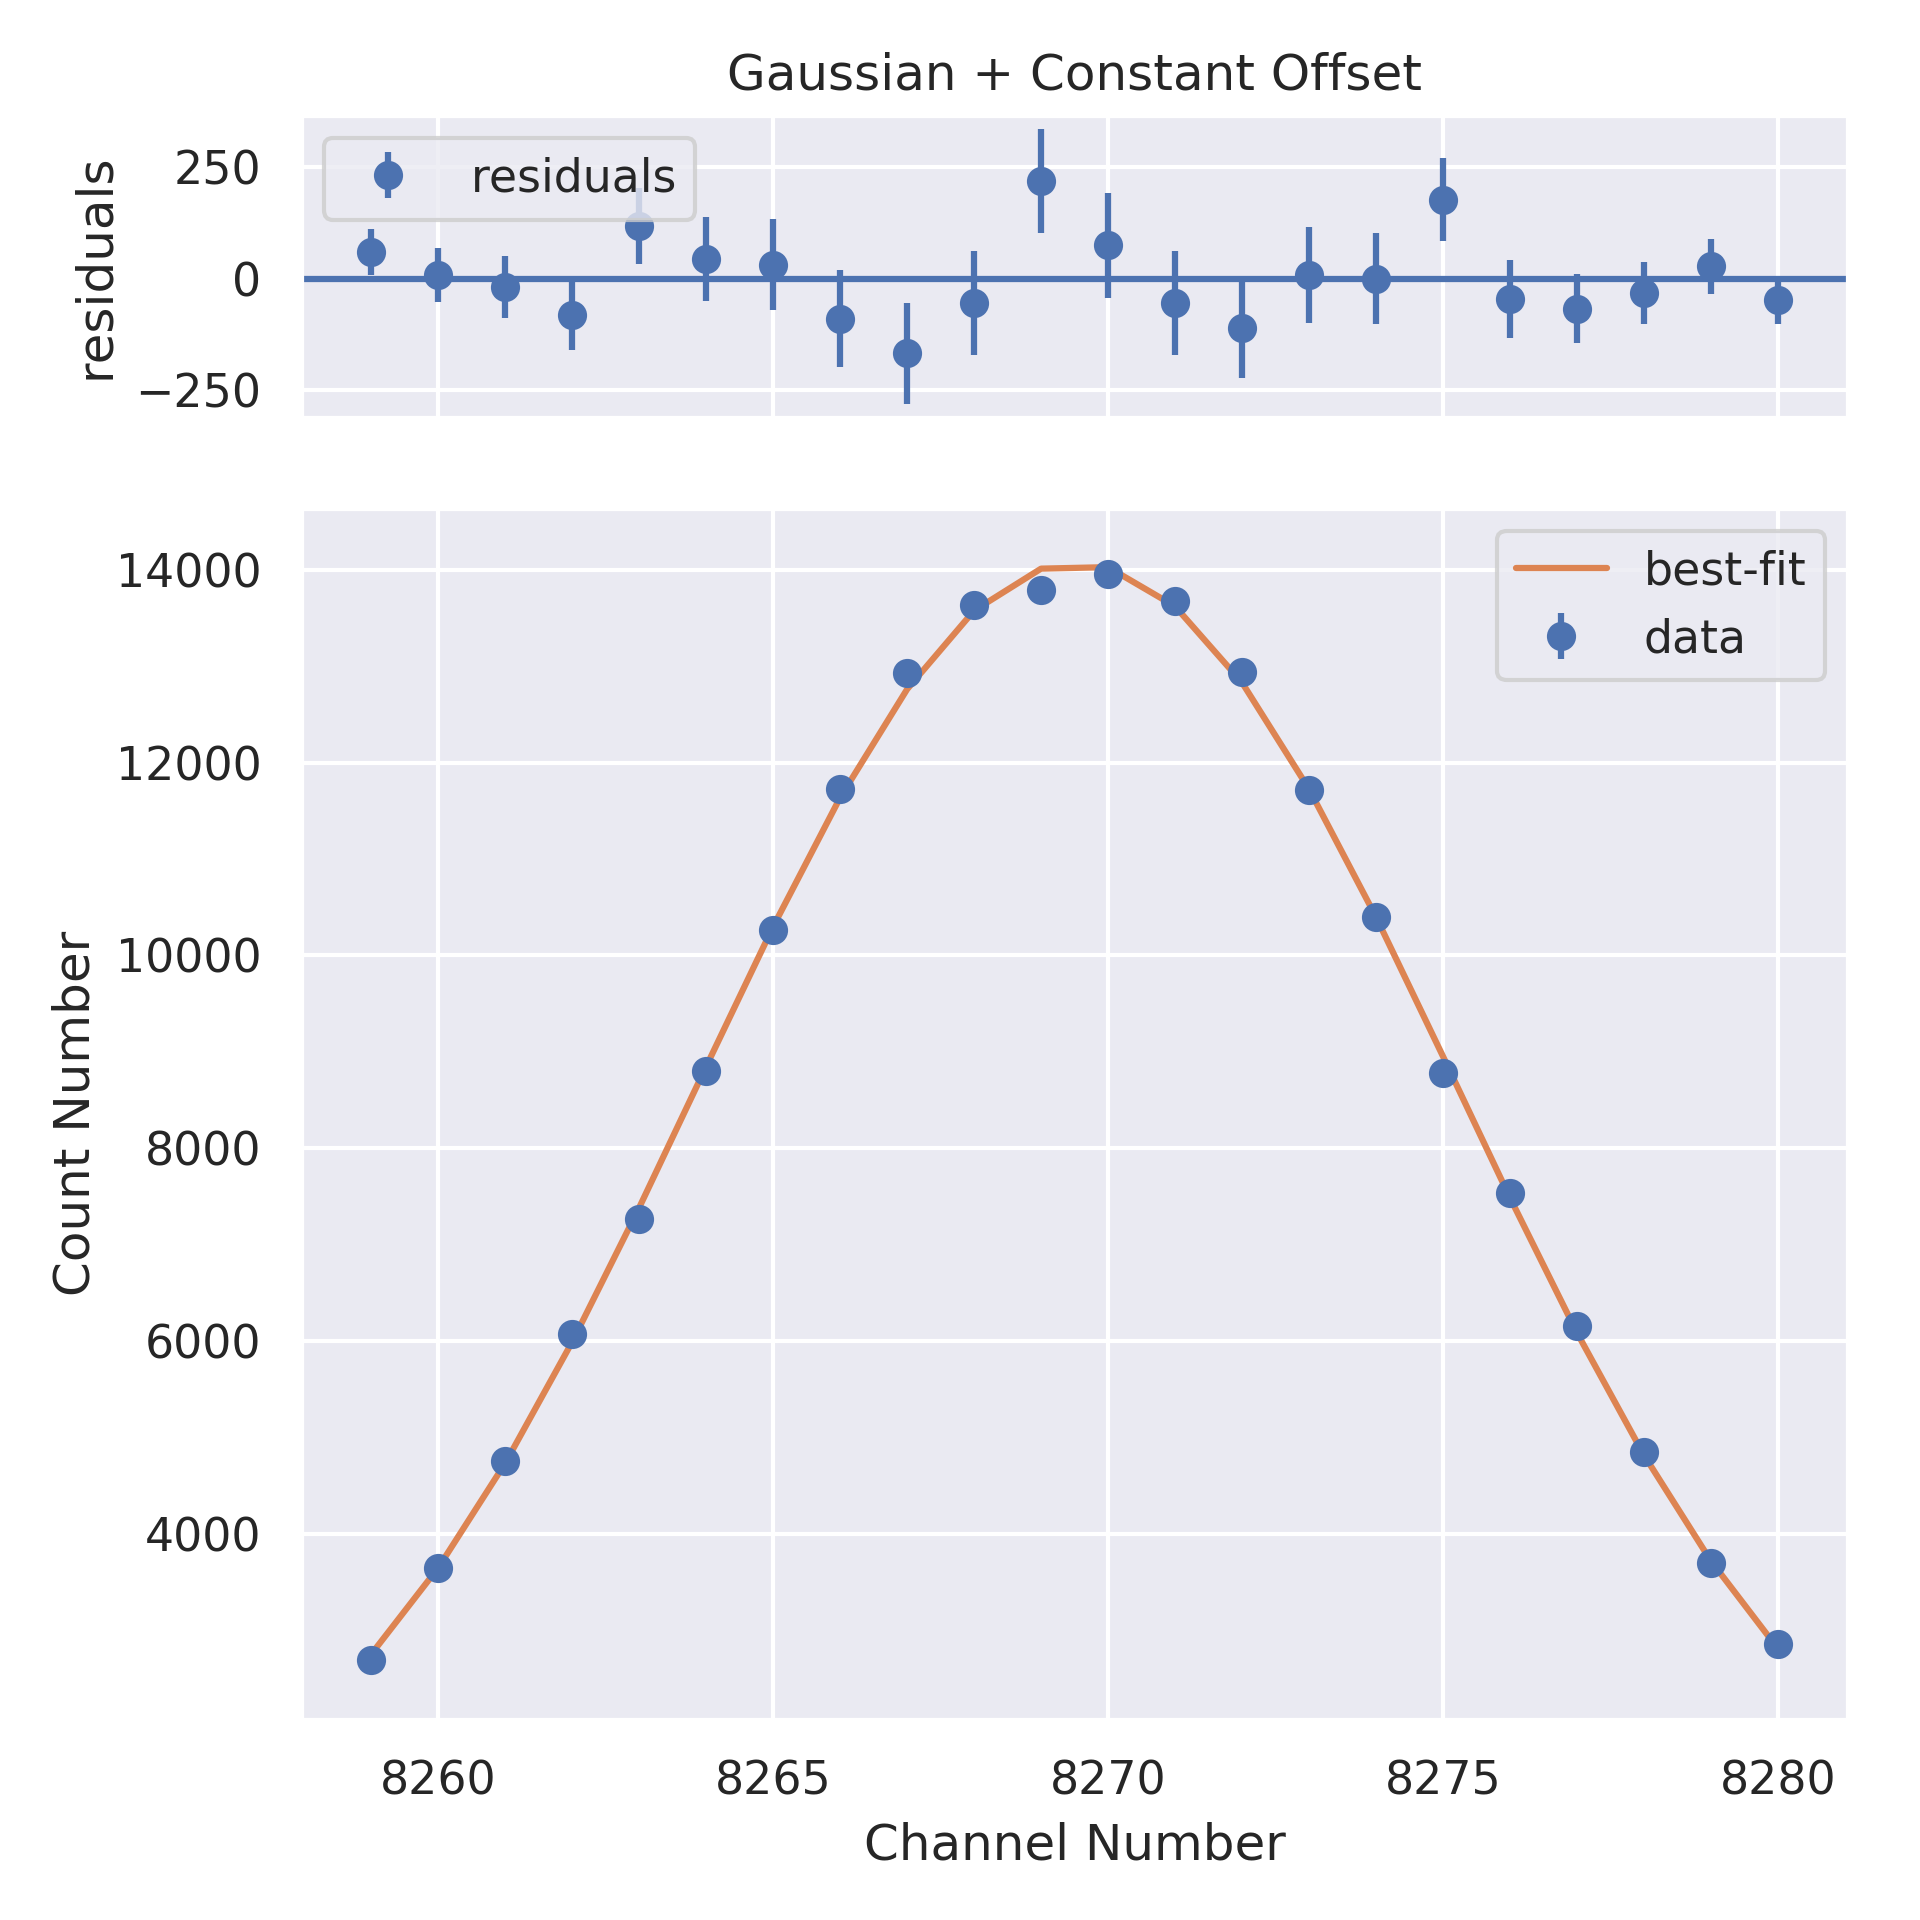
\includegraphics[width=\linewidth]{./Images/Cobalt60/Gauss/Gauss_1_Zoom.png}
    \caption{Zoomed in peak with fit. $\chi^2 = 18.66$, $\chi^2_\nu = 0.93$, \\ Prob = 54.42\%, $\mu = 8269.54$, $\sigma = 5.67$}
    %\label{fig:sub2}
  \end{subfigure}
  \caption{Fit of full \& zoomed in peak of \element{Co}{60} 1173 keV peak}
  %\label{fig:test}
\end{figure}
\begin{figure}[H]
  \centering
  \begin{subfigure}{.5\linewidth}
    \centering
    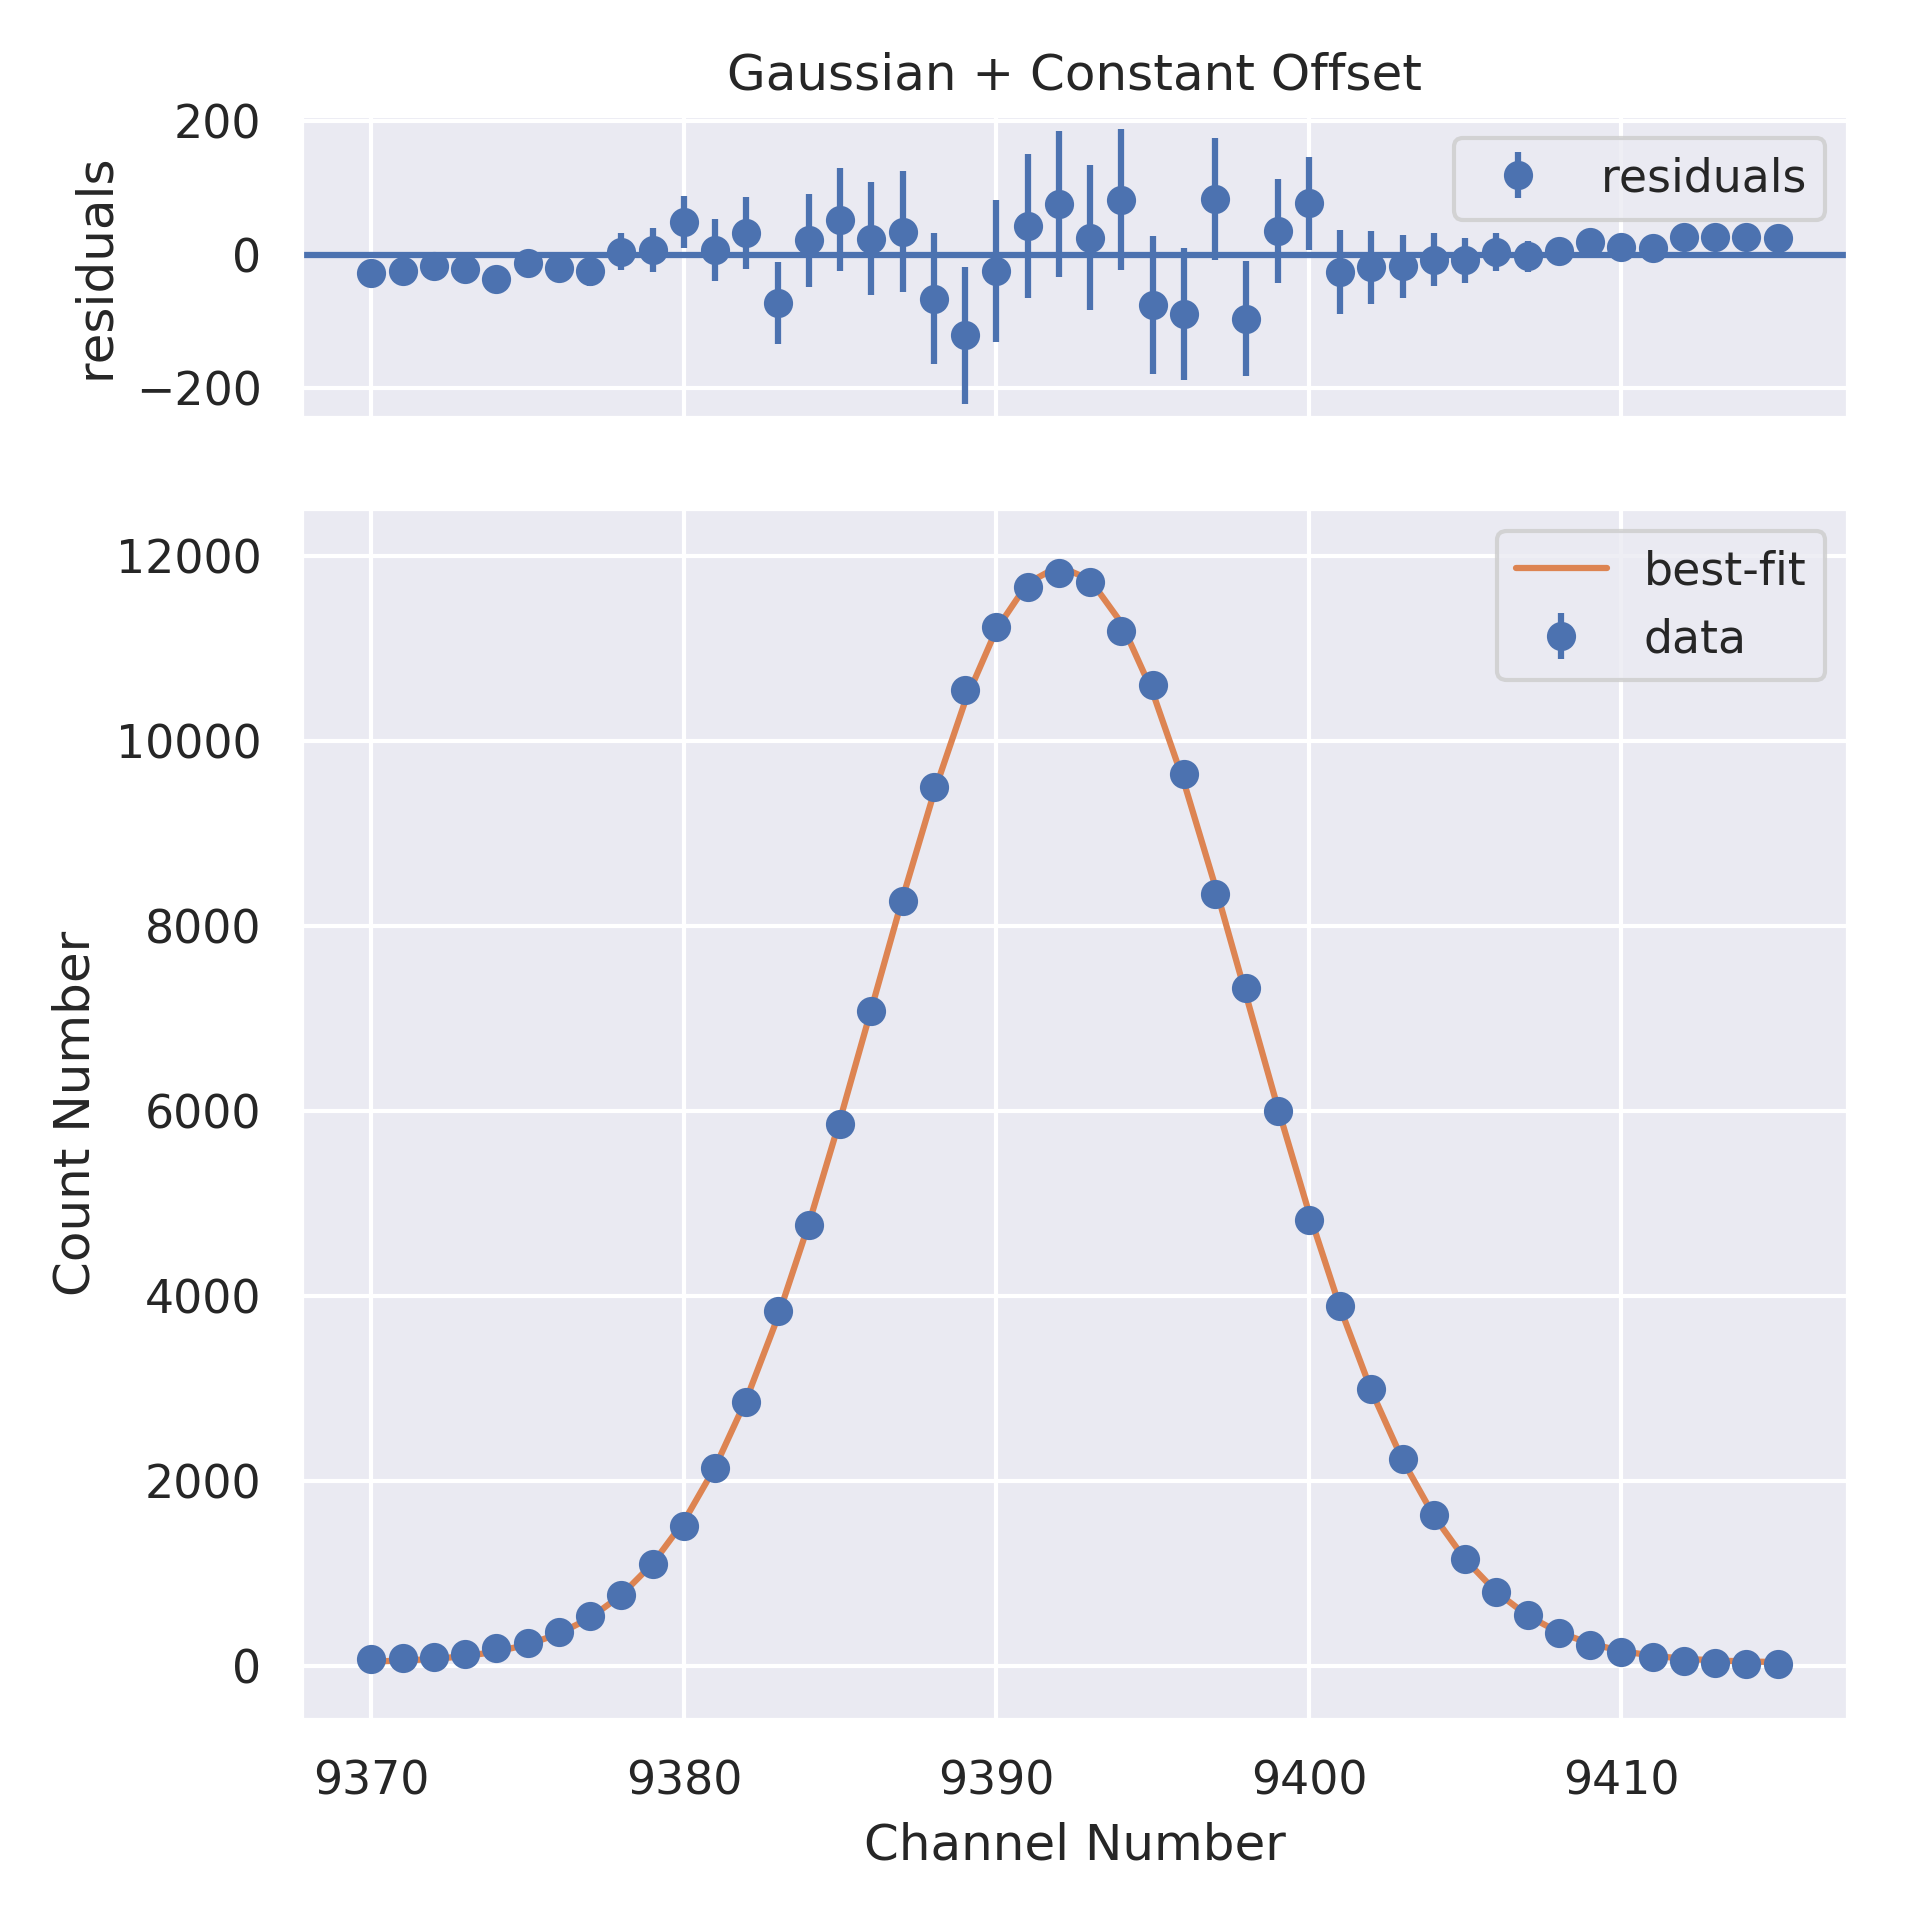
\includegraphics[width=\linewidth]{./Images/Cobalt60/Gauss/Gauss_2_Full.png}
    \caption{Full peak with fit. $\chi^2 = 173.52$, $\chi^2_\nu = 3.94$, \\ Prob = 0.00\%, $\mu = 9392.05$, $\sigma = 5.95$}
    %\label{fig:sub1}
  \end{subfigure}%
  \begin{subfigure}{.5\linewidth}
    \centering
    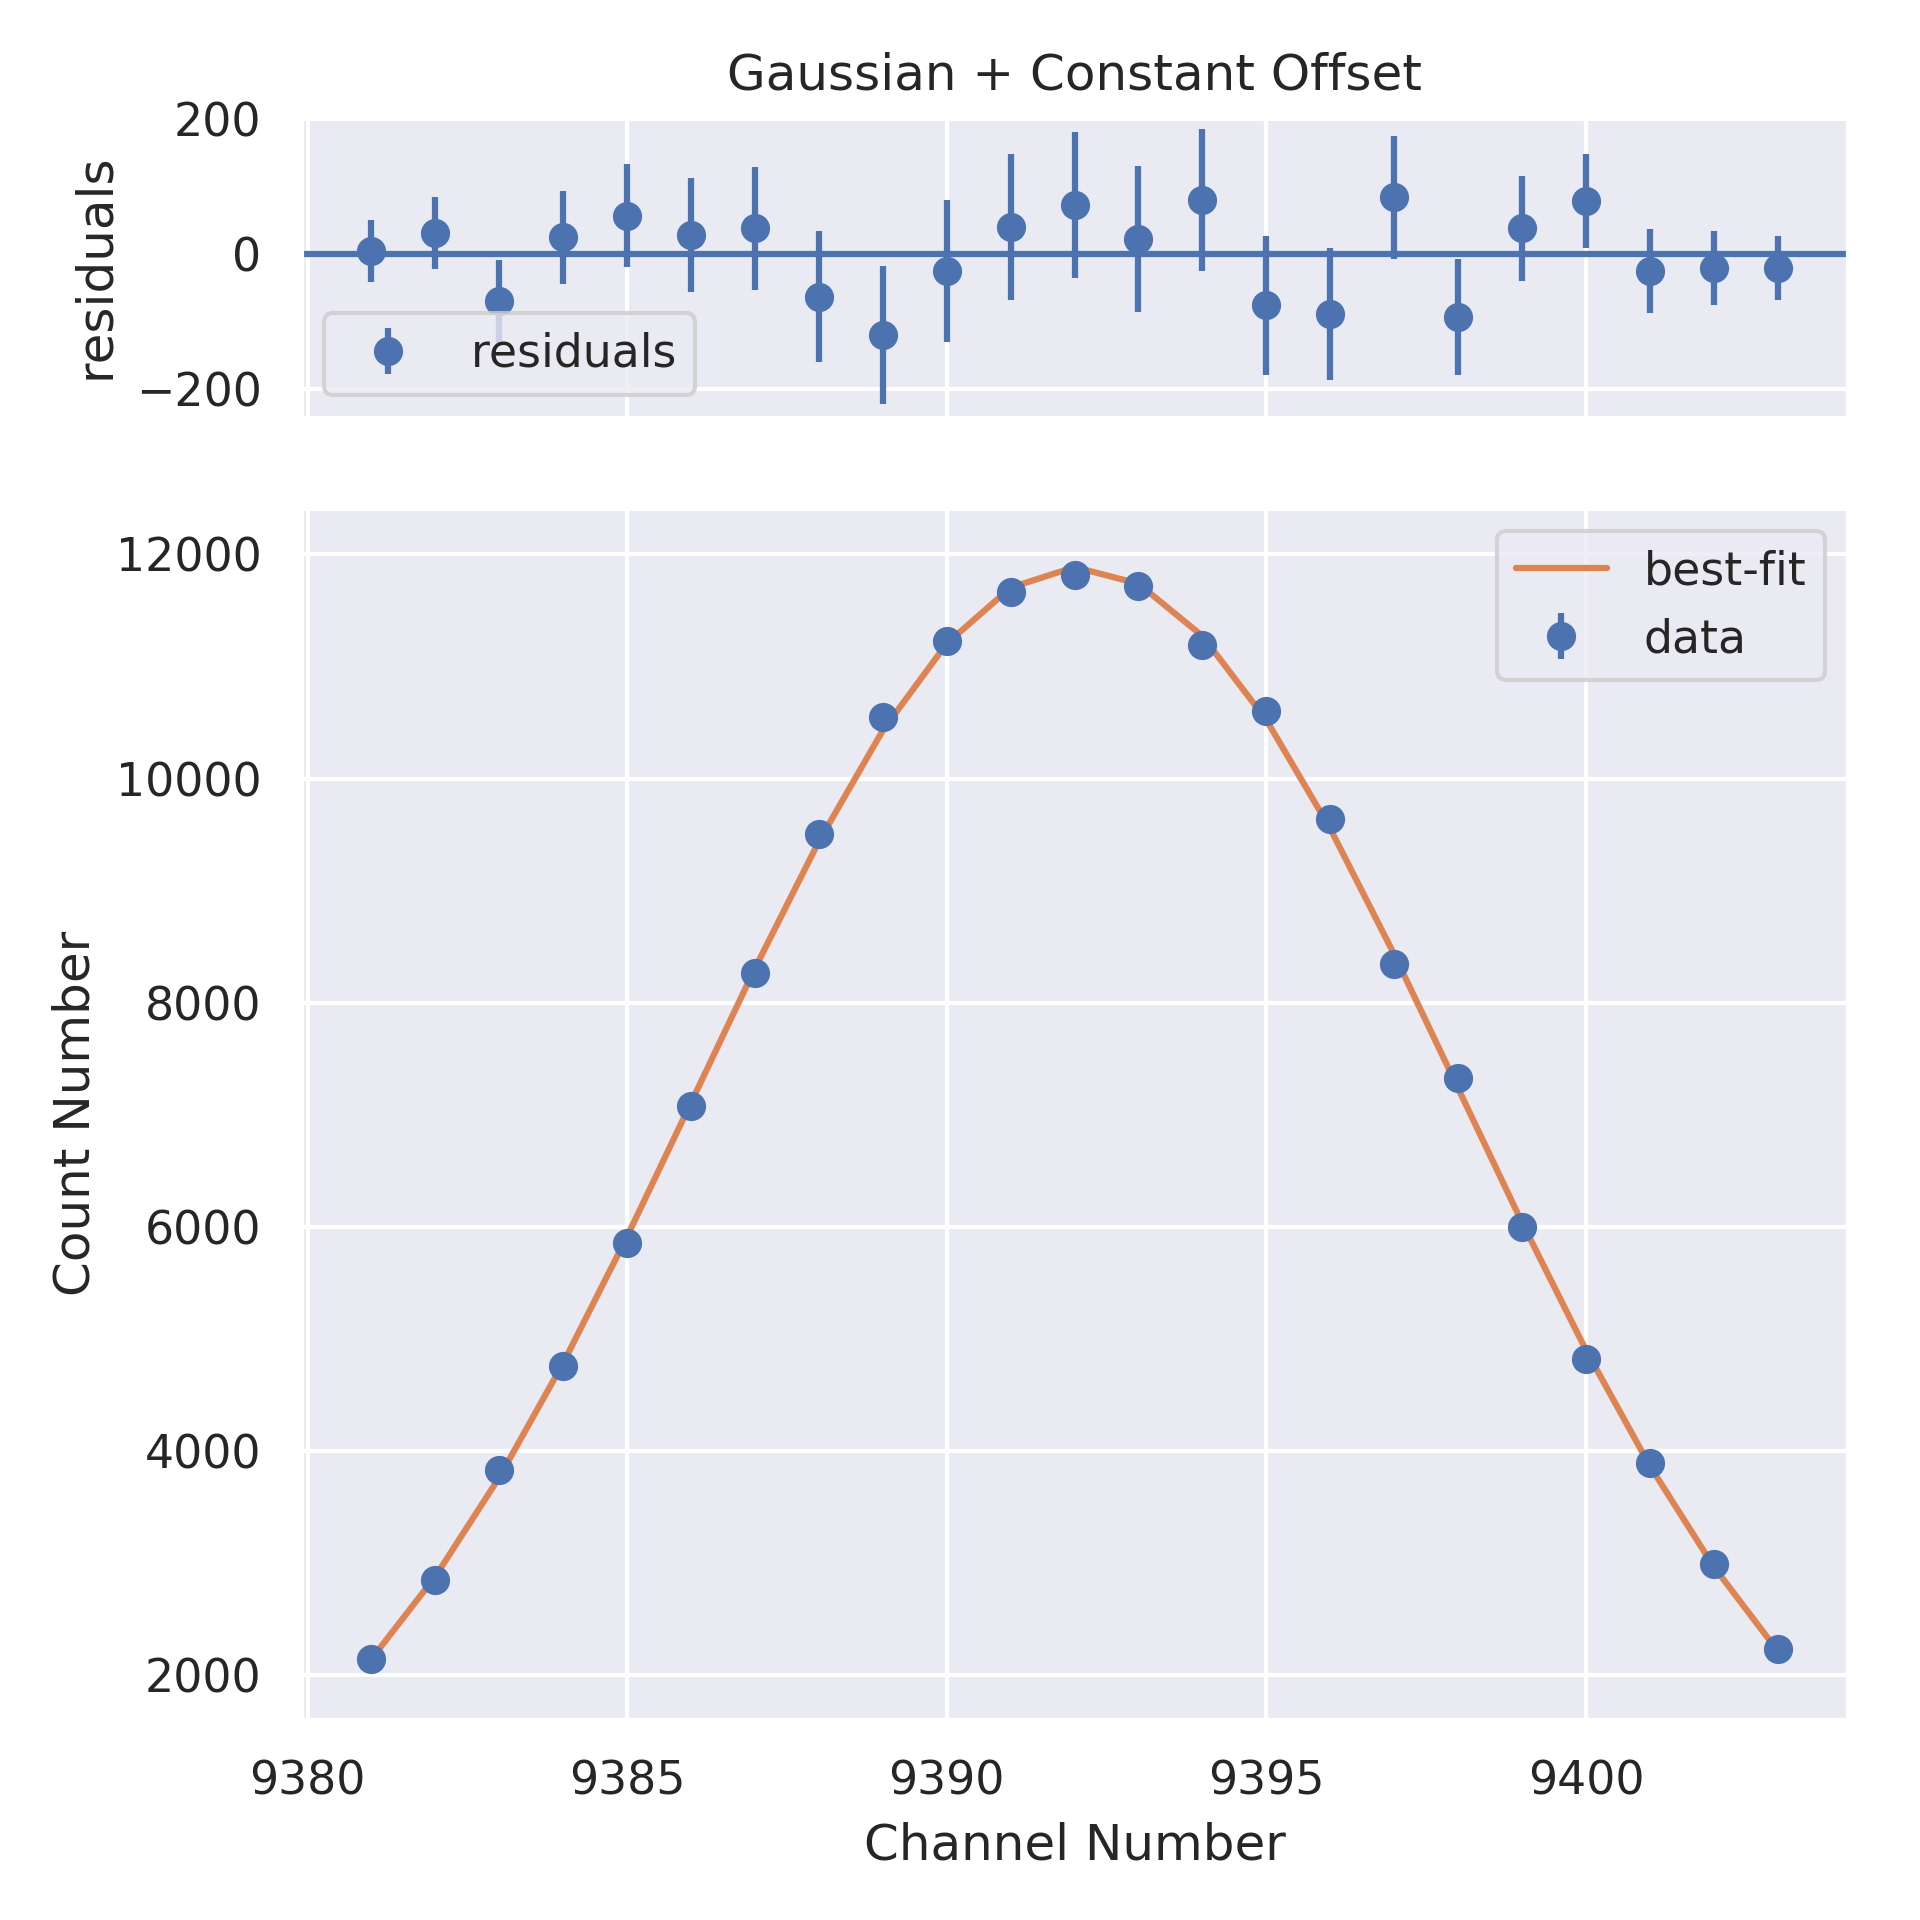
\includegraphics[width=\linewidth]{./Images/Cobalt60/Gauss/Gauss_2_Zoom.png}
    \caption{Zoomed in peak with fit. $\chi^2 = 11.12$, $\chi^2_\nu = 0.53$, \\ Prob = 96.04\%, $\mu = 9392.05$, $\sigma = 5.96$}
    %\label{fig:sub2}
  \end{subfigure}
  \caption{Fit of full \& zoomed in peak of \element{Co}{60} 1332 keV peak}
  %\label{fig:test}
\end{figure}
\clearpage
\subsubsection{Gaussian + Linear Fit}
\begin{figure}[H]
  \centering
  \begin{subfigure}{.5\linewidth}
    \centering
    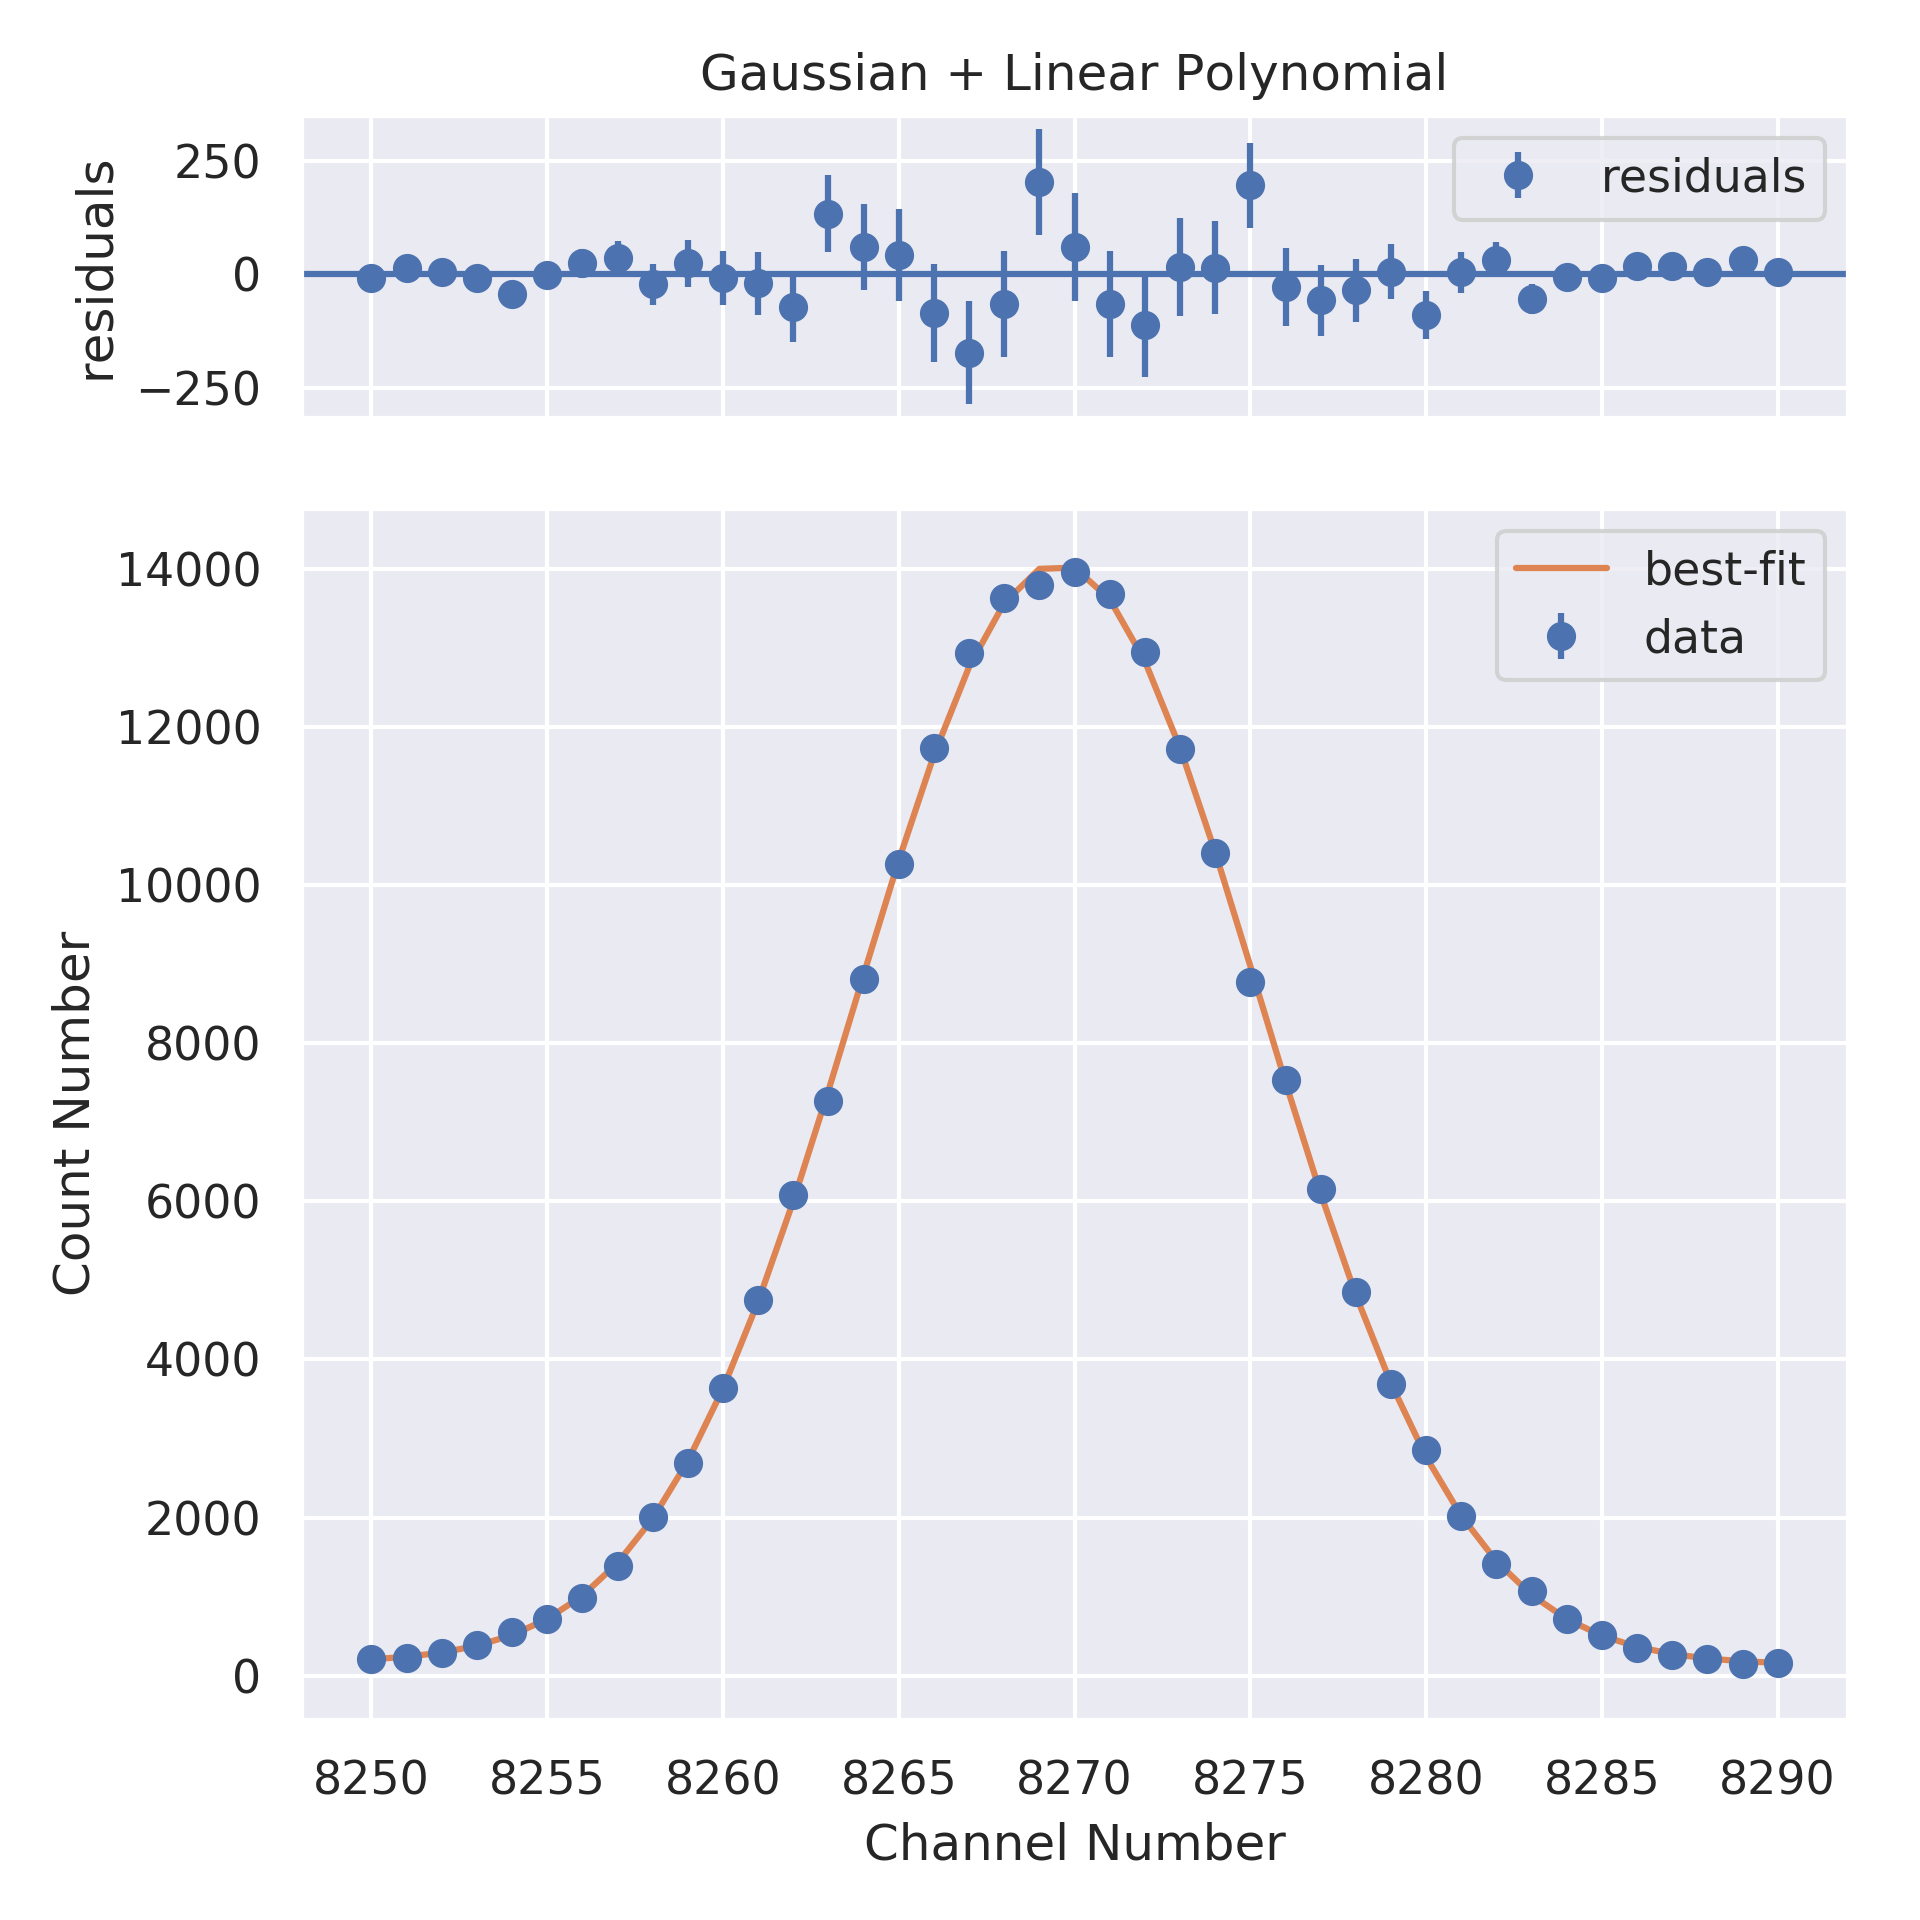
\includegraphics[width=\linewidth]{./Images/Cobalt60/Linear/Linear_1_Full.png}
    \caption{Full peak with fit. $\chi^2 = 39.06$, $\chi^2_\nu = 1.00$, \\ Prob = 46.72\%, $\mu = 8269.54$, $\sigma = 5.73$}
    %\label{fig:sub1}
  \end{subfigure}%
  \begin{subfigure}{.5\linewidth}
    \centering
    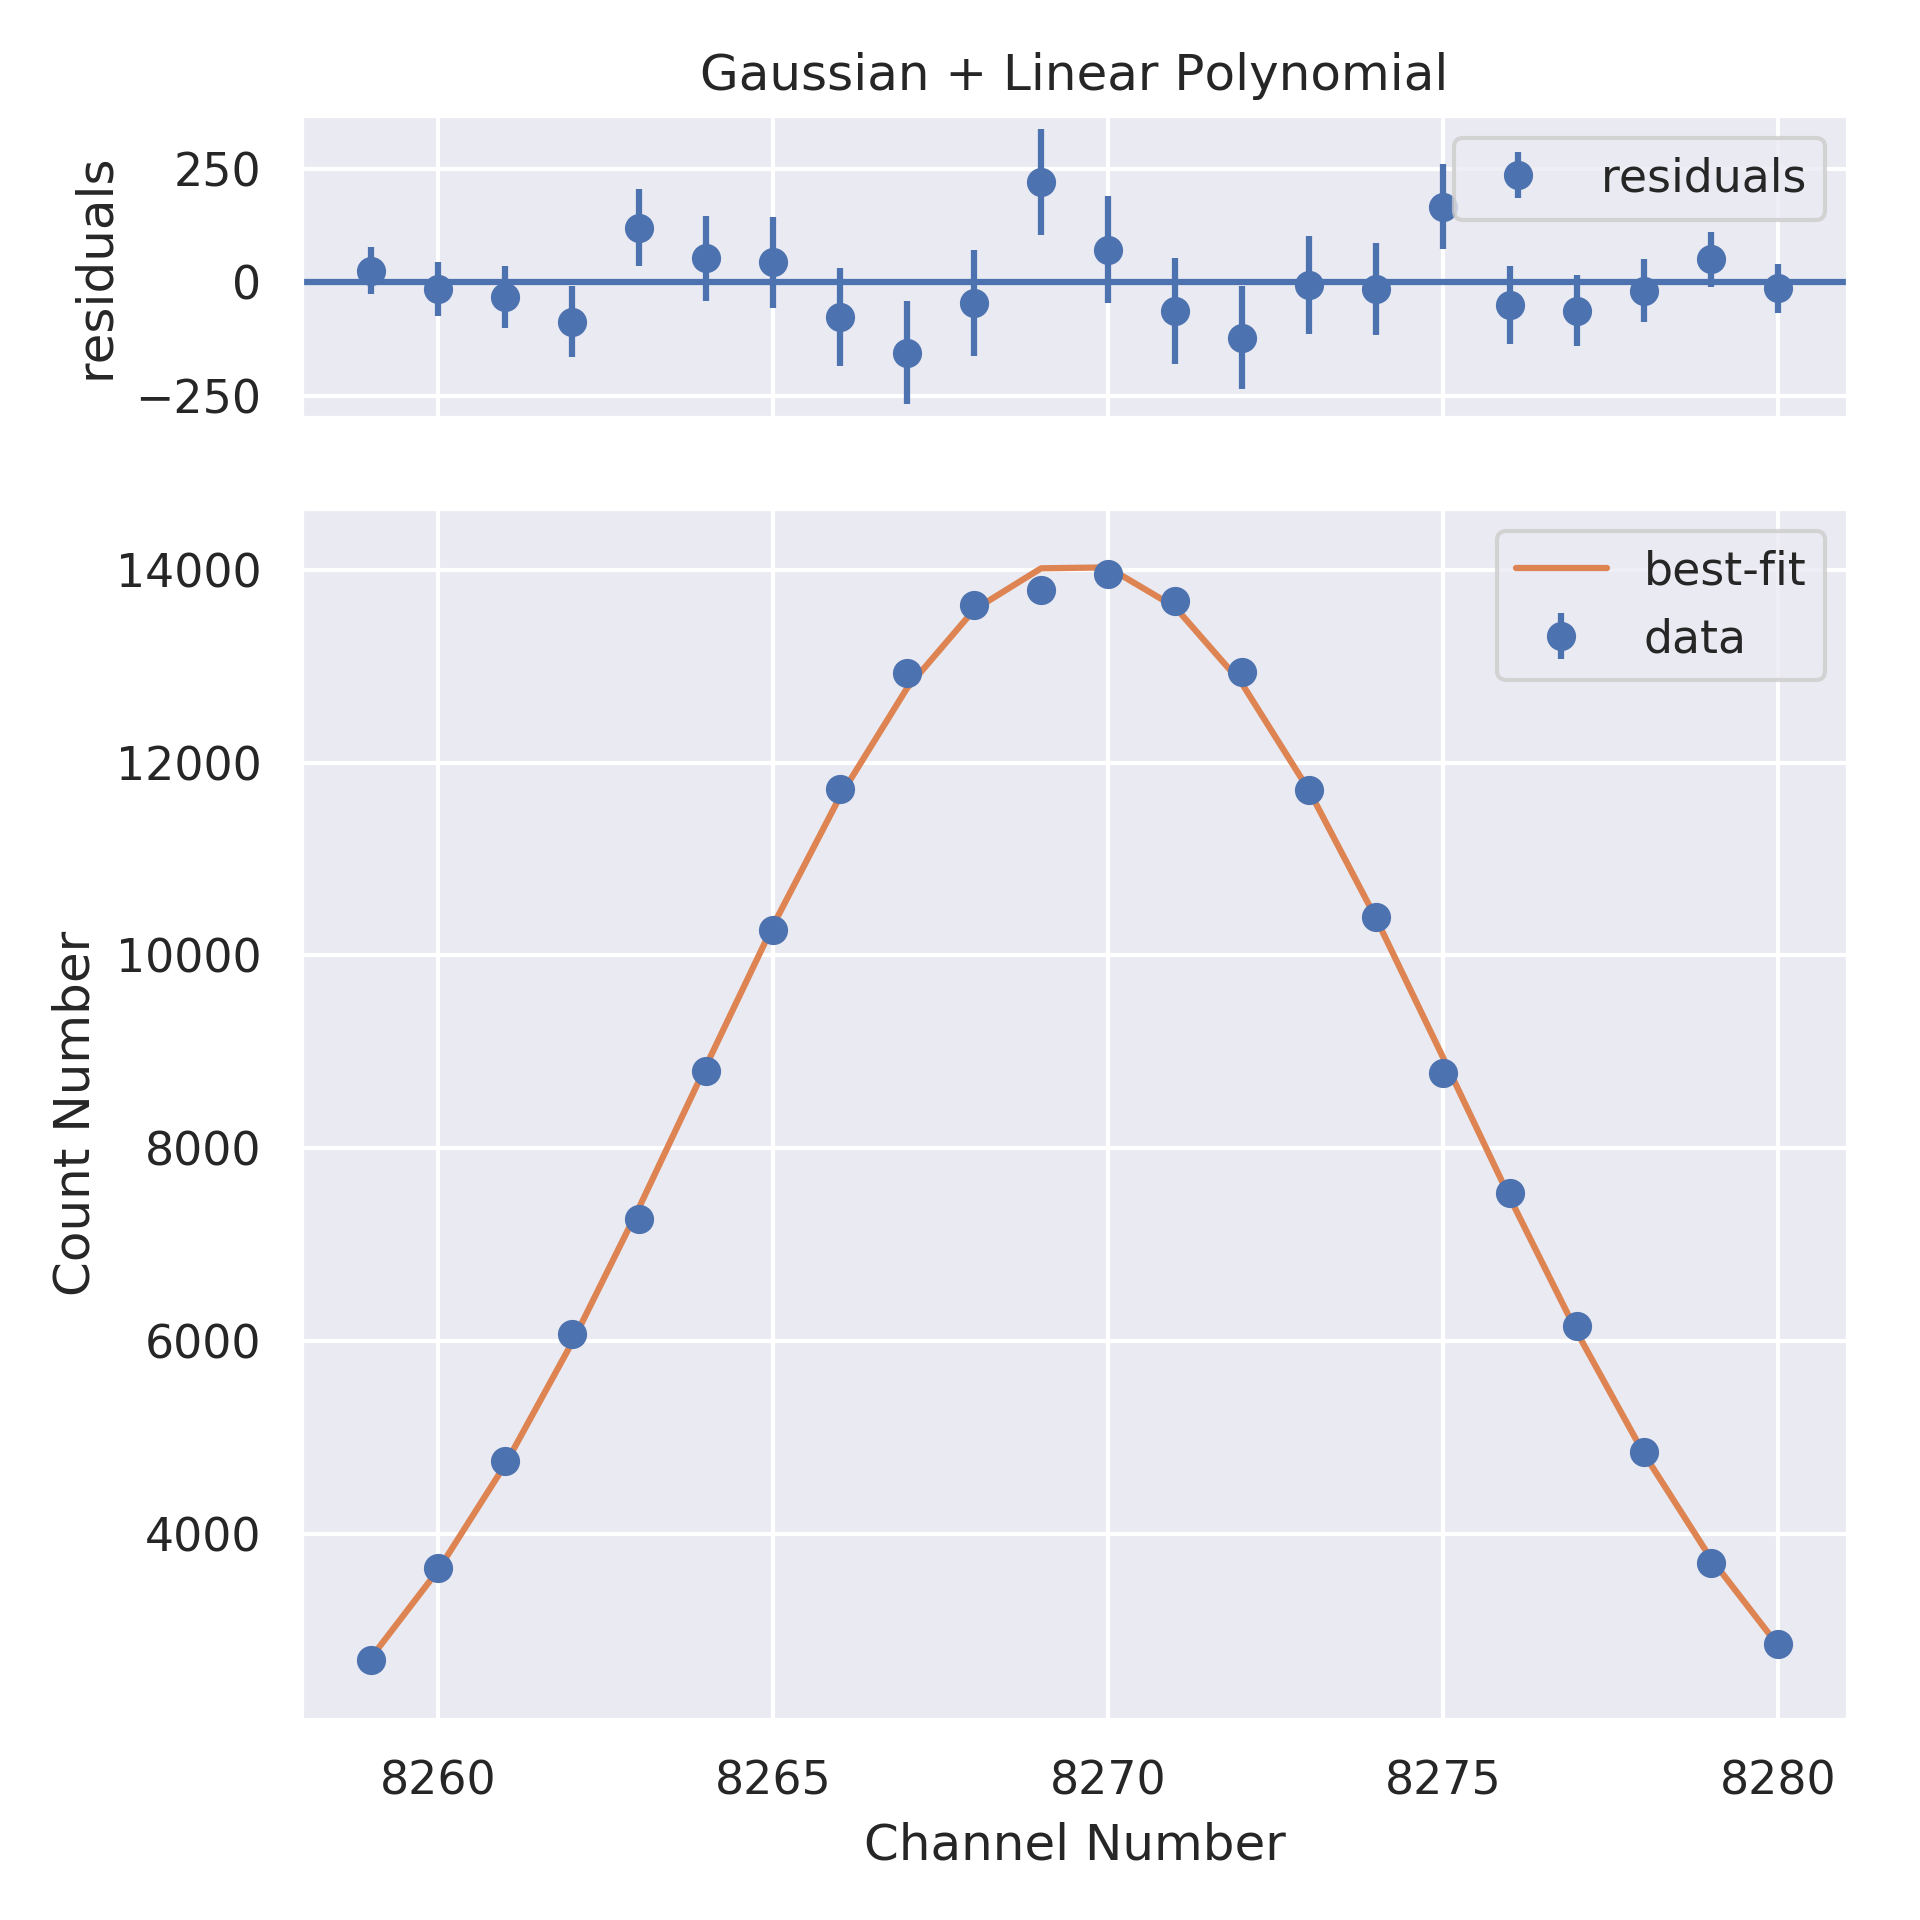
\includegraphics[width=\linewidth]{./Images/Cobalt60/Linear/Linear_1_Zoom.png}
    \caption{Zoomed in peak with fit. $\chi^2 = 17.24$, $\chi^2_\nu = 0.86$, \\ Prob = 63.72\%, $\mu = 8269.51$, $\sigma = 5.66$}
    %\label{fig:sub2}
  \end{subfigure}
  \caption{Fit of full \& zoomed in peak of \element{Co}{60} 1173 keV peak}
  %\label{fig:test}
\end{figure}
\begin{figure}[H]
  \centering
  \begin{subfigure}{.5\linewidth}
    \centering
    \includegraphics[width=\linewidth]{./Images/Cobalt60/Linear/Linear_2_Full.png}
    \caption{Full peak with fit. $\chi^2 = 36.11$, $\chi^2_\nu = 0.82$, \\ Prob = 79.53\%, $\mu = 9392.06$, $\sigma = 5.95$}
    %\label{fig:sub1}
  \end{subfigure}%
  \begin{subfigure}{.5\linewidth}
    \centering
    \includegraphics[width=\linewidth]{./Images/Cobalt60/Linear/Linear_2_Zoom.png}
    \caption{Zoomed in peak with fit. $\chi^2 = 10.89$, $\chi^2_\nu = 0.52$, \\ Prob = 96.49\%, $\mu = 9392.04$, $\sigma = 5.96$}
    %\label{fig:sub2}
  \end{subfigure}
  \caption{Fit of full \& zoomed in peak of \element{Co}{60} 1332 keV peak}
  %\label{fig:test}
\end{figure}
\clearpage
\subsubsection{Gaussian + Quadratic Fit}
\begin{figure}[H]
  \centering
  \begin{subfigure}{.5\linewidth}
    \centering
    \includegraphics[width=\linewidth]{./Images/Cobalt60/Quad/Quad_1_Full.png}
    \caption{Full peak with fit. $\chi^2 = 37.65$, $\chi^2_\nu = 0.97$, \\ Prob = 53.14\%, $\mu = 8269.54$, $\sigma = 5.71$}
    %\label{fig:sub1}
  \end{subfigure}%
  \begin{subfigure}{.5\linewidth}
    \centering
    \includegraphics[width=\linewidth]{./Images/Cobalt60/Quad/Quad_1_Zoom.png}
    \caption{Zoomed in peak with fit. $\chi^2 = 17.02$, $\chi^2_\nu = 0.85$, \\ Prob = 65.16\%, $\mu = 8269.51$, $\sigma = 5.57$}
    %\label{fig:sub2}
  \end{subfigure}
  \caption{Fit of full \& zoomed in peak of \element{Co}{60} 1173 keV peak}
  %\label{fig:test}
\end{figure}
\begin{figure}[H]
  \centering
  \begin{subfigure}{.5\linewidth}
    \centering
    \includegraphics[width=\linewidth]{./Images/Cobalt60/Quad/Quad_2_Full.png}
    \caption{Full peak with fit. $\chi^2 = 36.03$, $\chi^2_\nu = 0.82$, \\ Prob = 79.80\%, $\mu = 9392.06$, $\sigma = 5.95$}
    %\label{fig:sub1}
  \end{subfigure}%
  \begin{subfigure}{.5\linewidth}
    \centering
    \includegraphics[width=\linewidth]{./Images/Cobalt60/Quad/Quad_2_Zoom.png}
    \caption{Zoomed in peak with fit. $\chi^2 = 10.95$, $\chi^2_\nu = 0.52$, \\ Prob = 96.37\%, $\mu = 9392.04$, $\sigma = 6.32$}
    %\label{fig:sub2}
  \end{subfigure}
  \caption{Fit of full \& zoomed in peak of \element{Co}{60} 1332 keV peak}
  %\label{fig:test}
\end{figure}
\clearpage


\subsection{Sodium-22}
The \element{Na}{22} source had one medium energy peak, and one high-energy peak. Both of which were very distinctive, and so quite easy to fit for all functions.
\begin{figure}[H]
  \centering
  \includegraphics[width=0.95\linewidth]{./Images/Sodium22/Final_Sodium24hr.png}
  \caption{The final spectrum obtained for the \element{Na}{22} source run for 24 hours. This has been converted to energies by using the quadratic energy calibration.}
\end{figure} 
\subsubsection{Gaussian + Offset Fit}
\begin{figure}[H]
  \centering
  \begin{subfigure}{.5\linewidth}
    \centering
    \includegraphics[width=\linewidth]{./Images/Sodium22/Gauss/Gauss_1_Full.png}
    \caption{Full peak with fit. $\chi^2 = 202.42$, $\chi^2_\nu = 3.43$, \\ Prob = 0.00\%, $\mu = 3601.60$, $\sigma = 8.18$}
    %\label{fig:sub1}
  \end{subfigure}%
  \begin{subfigure}{.5\linewidth}
    \centering
    \includegraphics[width=\linewidth]{./Images/Sodium22/Gauss/Gauss_1_Zoom.png}
    \caption{Zoomed in peak with fit. $\chi^2 = 24.72$, $\chi^2_\nu = 0.82$, \\ Prob = 73.83\%, $\mu = 3601.60$, $\sigma = 7.88$}
    %\label{fig:sub2}
  \end{subfigure}
  \caption{Fit of full \& zoomed in peak of \element{Na}{22} 511 keV peak}
  %\label{fig:test}
\end{figure}
\begin{figure}[H]
  \centering
  \begin{subfigure}{.48\linewidth}
    \centering
    \includegraphics[width=\linewidth]{./Images/Sodium22/Gauss/Gauss_2_Full.png}
    \caption{Full peak with fit. $\chi^2 = 26.26$, $\chi^2_\nu = 0.80$, \\ Prob = 79.09\%, $\mu = 8983.57$, $\sigma = 5.79$}
    %\label{fig:sub1}
  \end{subfigure} 
  \begin{subfigure}{.48\linewidth}
    \centering
    \includegraphics[width=\linewidth]{./Images/Sodium22/Gauss/Gauss_2_Zoom.png}
    \caption{Zoomed in peak with fit. $\chi^2 = 9.38$, $\chi^2_\nu = 0.45$, \\ Prob = 98.59\%, $\mu = 8983.58$, $\sigma = 5.65$}
    %\label{fig:sub2}
  \end{subfigure}
  \caption{Fit of full \& zoomed in peak of \element{Na}{22} 1274 keV peak}
  %\label{fig:test}
\end{figure}
\clearpage
\subsubsection{Gaussian + Linear Fit}
\begin{figure}[H]
  \centering
  \begin{subfigure}{.5\linewidth}
    \centering
    \includegraphics[width=\linewidth]{./Images/Sodium22/Linear/Linear_1_Full.png}
    \caption{Full peak with fit. $\chi^2 = 197.63$, $\chi^2_\nu = 3.35$, \\ Prob = 0.00\%, $\mu = 3601.60$, $\sigma = 8.18$}
    %\label{fig:sub1}
  \end{subfigure}%
  \begin{subfigure}{.5\linewidth}
    \centering
    \includegraphics[width=\linewidth]{./Images/Sodium22/Linear/Linear_1_Zoom.png}
    \caption{Zoomed in peak with fit. $\chi^2 = 22.76$, $\chi^2_\nu = 0.76$, \\ Prob = 82.51\%, $\mu = 3601.55$, $\sigma = 7.88$}
    %\label{fig:sub2}
  \end{subfigure}
  \caption{Fit of full \& zoomed in peak of \element{Na}{60} 511 keV peak}
  %\label{fig:test}
\end{figure}
\begin{figure}[H]
  \centering
  \begin{subfigure}{.5\linewidth}
    \centering
    \includegraphics[width=\linewidth]{./Images/Sodium22/Linear/Linear_2_Full.png}
    \caption{Full peak with fit. $\chi^2 = 26.34$, $\chi^2_\nu = 0.80$, \\ Prob = 78.77\%, $\mu = 8983.58$, $\sigma = 5.79$}
    %\label{fig:sub1}
  \end{subfigure}%
  \begin{subfigure}{.5\linewidth}
    \centering
    \includegraphics[width=\linewidth]{./Images/Sodium22/Linear/Linear_2_Zoom.png}
    \caption{Zoomed in peak with fit. $\chi^2 = 9.41$, $\chi^2_\nu = 0.45$, \\ Prob = 98.56\%, $\mu = 8983.53$, $\sigma = 5.67$}
    %\label{fig:sub2}
  \end{subfigure}
  \caption{Fit of full \& zoomed in peak of \element{Na}{22} 1274 keV peak}
  %\label{fig:test}
\end{figure}
\clearpage
\subsubsection{Gaussian + Quadratic Fit}
\begin{figure}[H]
  \centering
  \begin{subfigure}{.5\linewidth}
    \centering
    \includegraphics[width=\linewidth]{./Images/Sodium22/Quad/Quad_1_Full.png}
    \caption{Full peak with fit.$\chi^2 = 90.05$, $\chi^2_\nu = 1.53$, \\ Prob = 0.57\%, $\mu = 3601.61$, $\sigma = 7.99$}
    %\label{fig:sub1}
  \end{subfigure}%
  \begin{subfigure}{.5\linewidth}
    \centering
    \includegraphics[width=\linewidth]{./Images/Sodium22/Quad/Quad_1_Zoom.png}
    \caption{Zoomed in peak with fit. $\chi^2 = 21.24$, $\chi^2_\nu = 0.71$, \\ Prob = 88.01\%, $\mu = 3601.55$, $\sigma = 7.04$}
    %\label{fig:sub2}
  \end{subfigure}
  \caption{Fit of full \& zoomed in peak of \element{Na}{60} 511 keV peak}
  %\label{fig:test}
\end{figure}
\begin{figure}[H]
  \centering
  \begin{subfigure}{.5\linewidth}
    \centering
    \includegraphics[width=\linewidth]{./Images/Sodium22/Quad/Quad_2_Full.png}
    \caption{Full peak with fit. $\chi^2 = 14.77$, $\chi^2_\nu = 0.45$, \\ Prob = 99.74\%, $\mu = 8983.58$, $\sigma = 5.62$}
    %\label{fig:sub1}
  \end{subfigure}%
  \begin{subfigure}{.5\linewidth}
    \centering
    \includegraphics[width=\linewidth]{./Images/Sodium22/Quad/Quad_2_Zoom.png}
    \caption{Zoomed in peak with fit. $\chi^2 = 9.55$, $\chi^2_\nu = 0.45$, \\ Prob = 98.41\%, $\mu = 8983.52$, $\sigma = 5.28$}
    %\label{fig:sub2}
  \end{subfigure}
  \caption{Fit of full \& zoomed in peak of \element{Na}{22} 1274 keV peak}
  %\label{fig:test}
\end{figure}

\clearpage

\section{Fit Comparisons}

Since there were three types of function fitted to the data, it is important that we identify which function both matched the data the best, and that is the simplest function. From functional analysis, we know that any function can be represented as an arbitrary sum of polynomials, and so by increasing the order of the fitted function will naturally cause better fit statistics, even though there is less physical reason to do so. Therefore, to find the ideal fitting function, we wanted to identify the lowest-order polynomial that correctly fitted the data, by showing that when we increase the order the fit remains the same, within errors.

This can be represented graphically by plotting the means produced for the same peaks of the different fits, with the error bars representing the standard deviation on the mean from the fit. If two error bars from different fits are overlapping with the means, then this shows that these fits are compatible with each other, and so the lowest order should be taken as the true fit. However, if they do not overlap, then this shows that they are not compatible, and so the higher order fit should be taken. 

\subsection{Barium-133}

\begin{figure}[H]
  \centering
  \includegraphics[width=0.95\linewidth]{./Images/Barium133/FitComparison_Peak1.png}
  \caption{Fit comparisons for \element{Ba}{133} 81 keV peak. Here is clear evidence that a simple Gaussian + offset fit is not sufficient, as the mean from the fit is significantly outside the acceptable area of the other two fits. This also shows that the linear polynomial provides no additional gain over the quadratic polynomial as both of their means coincide with each others error-bars, and so are statistically insignificant from each other. }
\end{figure}

\begin{figure}[H]
  \centering
  \includegraphics[width=0.95\linewidth]{./Images/Barium133/FitComparison_Peak2.png}
  \caption{Fit comparisons for \element{Ba}{133} 161 keV peak. Here, this shows all three means coincide with each other, and so for this particular peak going to anything above an offset has no advantage, however as other plots show that Gaussian + linear polynomial is best, that is what was used throughout.}
\end{figure}

\begin{figure}[H]
  \centering
  \includegraphics[width=0.95\linewidth]{./Images/Barium133/FitComparison_Peak3.png}
  \caption{Fit comparisons for \element{Ba}{133} 223 keV peak}
\end{figure}

\begin{figure}[H]
  \centering
  \includegraphics[width=0.95\linewidth]{./Images/Barium133/FitComparison_Peak4.png}
  \caption{Fit comparisons for \element{Ba}{133} 276 keV peak}
\end{figure}

\begin{figure}[H]
  \centering
  \includegraphics[width=0.95\linewidth]{./Images/Barium133/FitComparison_Peak5.png}
  \caption{Fit comparisons for \element{Ba}{133} 303 keV peak}
\end{figure}

\begin{figure}[H]
  \centering
  \includegraphics[width=0.95\linewidth]{./Images/Barium133/FitComparison_Peak6.png}
  \caption{Fit comparisons for \element{Ba}{133} 356 keV peak}
\end{figure}

\begin{figure}[H]
  \centering
  \includegraphics[width=0.95\linewidth]{./Images/Barium133/FitComparison_Peak7.png}
  \caption{Fit comparisons for \element{Ba}{133} 384 keV peak}
\end{figure}
\clearpage

\subsection{Cobalt-60}

\begin{figure}[H]
  \centering
  \includegraphics[width=0.95\linewidth]{./Images/Cobalt60/FitComparison_Peak1.png}
  \caption{Fit comparisons for \element{Co}{60} 1173 keV peak}
\end{figure}

\begin{figure}[H]
  \centering
  \includegraphics[width=0.95\linewidth]{./Images/Cobalt60/FitComparison_Peak2.png}
  \caption{Fit comparisons for \element{Co}{60} 1332 keV peak}
\end{figure}
\clearpage

\subsection{Sodium-22}
\begin{figure}[H]
  \centering
  \includegraphics[width=0.95\linewidth]{./Images/Sodium22/FitComparison_Peak1.png}
  \caption{Fit comparisons for \element{Na}{22} 511 keV peak}
\end{figure}

\begin{figure}[H]
  \centering
  \includegraphics[width=0.95\linewidth]{./Images/Sodium22/FitComparison_Peak2.png}
  \caption{Fit comparisons for \element{Na}{22} 1274 keV peak}
\end{figure}
\clearpage

\section{Python Code}
Below is the complete collection of our Python codes that we wrote during the four weeks of our experiment to run various data analysis tools on the raw data, including curve fitting, energy calibration and detector resolution finding. They are included in this appendix so that way we have them on records, in case something tragic happens to the digital copies stored on the central university file system. 

However, we have also mitigated against file loss by uploading our Python files, raw data, and this appendix to a GitHub repository that is hosted externally. In addition to being used as a version tracker tool helping us identify changes made to the codes over time (as we add, change \& remove features), it also provides mitigation against file loss as the current builds can simply be downloaded from the repo again. This also provides an easy way for others to double check figures or results, if they so desire -- improving transparency for our experiment, which is something that all scientists should be striving to do. 

GitHub: \texttt{https://github.com/AlexMaraio/HPGeDetector}


\subsection{GaussianFit.py}
This file is the file responsible for the fitting of the individual Gaussians to the peaks in the data. Here, we also add various order polynomials in addition to the Gaussian, starting from a simple offset to a quadratic order polynomial. This adjusts the way the fit works in subtle ways and we needed to see how fitting the various functions worked. Of course any arbitrary function can be approximated as a linear polynomial of arbitrary degree, so naturally going to a higher order polynomial will increase the goodness of fit, however detract from what can be extracted from the fit. 

By looking how the mean changes between the different fit types we can determine if we are justified in increasing the order of the polynomial, and after our analysis thanks to the following code, we can not justify going beyond a linear polynomial in addition to the Gaussian function.

\begin{minted}[linenos,tabsize=2,breaklines,breakanywhere]{python}
import numpy as np
import matplotlib.pylab as plt
import seaborn as sns
sns.set()
import scipy.optimize as sciopt
import scipy.stats as scistats
from lmfit import Model, Parameters
import pandas as pd

def ChiSqFunc(Measured,Fitted,Errors):
  ChiSquared = 0
  for i in range(len(Measured)):
    ChiSquared += ((Measured[i] - Fitted[i])**2.0) / ((Errors[i])**2.0)
  ReducedChiSq = ChiSquared/(len(Measured)-2)
  ProbChiSq = (1.0 - scistats.chi2.cdf(ChiSquared,len(Measured)-2) )  * 100.0
  return ChiSquared, ReducedChiSq, ProbChiSq

def Gauss(x,A,mean,sigma,a):
  return (A/(np.sqrt(2*np.pi) * sigma )) *np.exp(-((x-mean)**2.0)/(2.0*(sigma**2.0))) + a

def GaussLinear(x,A,mean,sigma,a,b):
  return (A/(np.sqrt(2*np.pi) * sigma ))*np.exp(-((x-mean)**2.0)/(2.0*(sigma**2.0))) + a + b*x

def GaussQuad(x,A,mean,sigma,a,b,c):
  return (A/(np.sqrt(2*np.pi) * sigma ))*np.exp(-((x-mean)**2.0)/(2.0*(sigma**2.0))) + a + b*x + c*x**2.0    

def ChToEnergy(Ch,a,b,c):
  Energy = np.sqrt( ( (Ch - c + (b**2.0 / (4*a))) )/a ) - (b / (2*a))
  return Energy

SetSigma = 2

BariumList = [ [[550,585,570,81],[1125,1140,1132,161],[1565,1582,1574,223],[1935,1960,1948,276],[2118,2150,2135,303],[2493,2526,2509,356],[2688,2723,2705,384]] , [] ]
SodiumList = [ [ [3570,3630,3600,511] , [8966,9000,8984,1274]] , [] ]
CobaltList = [ [ [8250,8290,8270,1173] , [9370,9415,9392,1332]] , [] ]

SourceList = ["Barium133-24HrRun_006_eh_1","Sodium22-24HrData_002_eh_1","Cobalt60-24HrData_004_eh_1"]

PlotResolution = 300

PeakNo = int(1)

datadict = {'Element':[],'Fit type':[], 'Peak number':[], 'Peak type':[], 'Energy (keV)': [], 'Resolution':[], 'Min of range':[], 'Max of range':[], 'Mean':[], 'A':[], 'Sigma':[], 'Error on mean':[], 'a':[], 'b':[], 'c':[], 'chisq':[], 'Reduced chisq':[], 'Probchisq':[]}

# Fit parameters
a = 2.63977565e-06
b = 7.04767648
c = -1.91414134e-01

for source in SourceList:
  if source == "Barium133-24HrRun_006_eh_1":
    ElementList = BariumList
    Element = "Barium133"
  elif source == "Sodium22-24HrData_002_eh_1":
    ElementList = SodiumList
    Element = "Sodium22"
  else:
    ElementList = CobaltList
    Element = "Cobalt60"

  for item in ElementList:
    for peak in item:
      #! Initialises the source and ranges for run

      if item == ElementList[0]:
        PeakType = "Full"
      else:
        PeakType = "Zoom"

      df = pd.read_csv(source + ".dat", sep = r"\s+", names = ['channel number','count number'])

      df['count errors'] = np.sqrt(df['count number'])
      df['count errors'] = df['count errors'].replace(0,1)

      MinValue = peak[0]
      MaxValue = peak[1]
      MeanValue = peak[2]
      PeakEnergy = peak[3]

      data = df[(MinValue<=df['channel number']) & (df['channel number']<=MaxValue)]
      #-----------------------------------------------------------------------------
      #! Gaussian + Offset model only

      GaussModel = Model(Gauss)
      Params = Parameters()

      Params.add('A',value=max(data['count number']),vary=True,min=0)
      Params.add('mean',value=MeanValue,vary=True)
      Params.add('sigma',value=1,vary=True)
      Params.add('a',value=1,vary=True)

      FitResult = GaussModel.fit(data['count number'],params=Params,x=data['channel number'])
      TempList = [ FitResult.best_values['mean'] - SetSigma *FitResult.best_values['sigma'] , FitResult.best_values['mean'] + SetSigma *FitResult.best_values['sigma'] , FitResult.best_values['mean'] , PeakEnergy ] 
      if item == ElementList[0]:
        ElementList[1].append(TempList)
      #print(FitResult.best_values)
      FitResult.plot(yerr=data['count errors'],xlabel='Channel Number',ylabel='Count Number',title='Gaussian + Constant Offset')

      ChiStats = ChiSqFunc(list(data['count number']),list(FitResult.best_fit),list(data['count errors']))

      plt.tight_layout()
      plt.savefig(f'Plots/{Element}/Gauss/Gauss_{PeakNo}_{PeakType}.png', format='png', dpi=PlotResolution)
      plt.close('all')

      CountMax1 = FitResult.best_values['A'] / ( FitResult.best_values['sigma'] * np.sqrt(2 * np.pi ) ) + FitResult.best_values['a']
      ErrorOnMean1 = FitResult.best_values['sigma'] / np.sqrt(CountMax1)

      datadict['Element'].append(Element)
      datadict['Fit type'].append('Gauss')
      datadict['Energy (keV)'].append(PeakEnergy)
      FWHM_Energy = 2 * np.sqrt(2*np.log(2)) * ChToEnergy(FitResult.best_values['sigma'],a,b,c)
      datadict['Resolution'].append( FWHM_Energy / PeakEnergy)
      #datadict['Resolution'].append( ( (2 * np.sqrt(2*np.log(2))*FitResult.best_values['sigma'] - b ) / a ) / PeakEnergy)
      datadict['Peak number'].append(PeakNo)
      datadict['Peak type'].append(PeakType)
      datadict['Min of range'].append(MinValue)
      datadict['Max of range'].append(MaxValue)
      datadict['Mean'].append(FitResult.best_values['mean'])
      datadict['A'].append(FitResult.best_values['A'])
      datadict['Sigma'].append(FitResult.best_values['sigma'])
      datadict['Error on mean'].append(1)
      datadict['a'].append(FitResult.best_values['a'])
      datadict['b'].append(0)
      datadict['c'].append(0)
      datadict['chisq'].append(ChiStats[0])
      datadict['Reduced chisq'].append(ChiStats[1])
      datadict['Probchisq'].append(ChiStats[2])

      
      #-----------------------------------------------------------------------------
      #! Gaussain + Linear model 

      GaussModel2 = Model(GaussLinear)
      Params2 = Parameters()

      Params2.add('A',value=max(data['count number']),vary=True,min=0)
      Params2.add('mean',value=MeanValue,vary=True)
      Params2.add('sigma',value=1,vary=True)
      Params2.add('a',value=1,vary=True)
      Params2.add('b',value=1,vary=True)

      FitResult2 = GaussModel2.fit(data['count number'],params=Params2,x=data['channel number'])
      FitResult2.plot(yerr=data['count errors'],xlabel='Channel Number',ylabel='Count Number',title='Gaussian + Linear Polynomial')

      ChiStats2 = ChiSqFunc(list(data['count number']),list(FitResult2.best_fit),list(data['count errors']))

      plt.tight_layout()
      plt.savefig(f'Plots/{Element}/Linear/Linear_{PeakNo}_{PeakType}.png', format='png', dpi=PlotResolution)
      plt.close('all')

      CountMax2 = FitResult2.best_values['A'] / ( FitResult2.best_values['sigma'] * np.sqrt(2 * np.pi ) ) + FitResult2.best_values['a'] + FitResult2.best_values['b'] * FitResult2.best_values['mean']
      ErrorOnMean2 = FitResult2.best_values['sigma'] / np.sqrt(CountMax2)
      
      datadict['Element'].append(Element)
      datadict['Fit type'].append('Linear')
      datadict['Energy (keV)'].append(PeakEnergy)
      FWHM_Energy = 2 * np.sqrt(2*np.log(2)) * ChToEnergy(FitResult2.best_values['sigma'],a,b,c)
      datadict['Resolution'].append( FWHM_Energy / PeakEnergy)
      datadict['Peak number'].append(PeakNo)
      datadict['Peak type'].append(PeakType)
      datadict['Min of range'].append(MinValue)
      datadict['Max of range'].append(MaxValue)
      datadict['Mean'].append(FitResult2.best_values['mean'])
      datadict['A'].append(FitResult2.best_values['A'])
      datadict['Sigma'].append(FitResult2.best_values['sigma'])
      datadict['Error on mean'].append(1)
      datadict['a'].append(FitResult2.best_values['a'])
      datadict['b'].append(FitResult2.best_values['b'])
      datadict['c'].append(0)
      datadict['chisq'].append(ChiStats2[0])
      datadict['Reduced chisq'].append(ChiStats2[1])
      datadict['Probchisq'].append(ChiStats2[2])

      #-----------------------------------------------------------------------------
      #! Gaussain + Quadratic model 

      GaussModel3 = Model(GaussQuad)
      Params3 = Parameters()

      Params3.add('A',value=max(data['count number']),vary=True,min=0)
      Params3.add('mean',value=MeanValue,vary=True)
      Params3.add('sigma',value=1,vary=True)
      Params3.add('a',value=1,vary=True)
      Params3.add('b',value=1,vary=True)
      Params3.add('c',value=1,vary=True)

      FitResult3 = GaussModel3.fit(data['count number'],params=Params3,x=data['channel number'])
      FitResult3.plot(yerr=data['count errors'],xlabel='Channel Number',ylabel='Count Number',title='Gaussian + Quadratic Polynomial')

      ChiStats3 = ChiSqFunc(list(data['count number']),list(FitResult3.best_fit),list(data['count errors']))

      plt.tight_layout()
      plt.savefig(f'Plots/{Element}/Quad/Quad_{PeakNo}_{PeakType}.png', format='png', dpi=PlotResolution)
      plt.close('all')

      CountMax3 = FitResult3.best_values['A'] / ( FitResult3.best_values['sigma'] * np.sqrt(2 * np.pi ) ) + FitResult3.best_values['a'] + FitResult3.best_values['b'] * FitResult3.best_values['mean'] + FitResult3.best_values['c'] * (FitResult3.best_values['mean'])** 2.0
      ErrorOnMean3 = FitResult3.best_values['sigma'] / np.sqrt(CountMax3)

      datadict['Element'].append(Element)
      datadict['Fit type'].append('Quad')
      datadict['Energy (keV)'].append(PeakEnergy)
      FWHM_Energy = 2 * np.sqrt(2*np.log(2)) * ChToEnergy(FitResult3.best_values['sigma'],a,b,c)
      datadict['Resolution'].append( FWHM_Energy / PeakEnergy)
      datadict['Peak number'].append(PeakNo)
      datadict['Peak type'].append(PeakType)
      datadict['Min of range'].append(MinValue)
      datadict['Max of range'].append(MaxValue)
      datadict['Mean'].append(FitResult3.best_values['mean'])
      datadict['A'].append(FitResult3.best_values['A'])
      datadict['Sigma'].append(FitResult3.best_values['sigma'])
      datadict['Error on mean'].append(1)
      datadict['a'].append(FitResult3.best_values['a'])
      datadict['b'].append(FitResult3.best_values['b'])
      datadict['c'].append(FitResult3.best_values['c'])
      datadict['chisq'].append(ChiStats3[0])
      datadict['Reduced chisq'].append(ChiStats3[1])
      datadict['Probchisq'].append(ChiStats3[2])
      

      Delta12 = np.abs(FitResult.best_values['mean'] - FitResult2.best_values['mean'])
      ErrorDelta12 = np.sqrt( ErrorOnMean1**2.0 + ErrorOnMean2**2.0 )

      Delta23 = np.abs(FitResult2.best_values['mean'] - FitResult3.best_values['mean'])
      ErrorDelta23 = np.sqrt( ErrorOnMean2**2.0 + ErrorOnMean3**2.0 )


      if PeakType == "Zoom":
        if abs(ErrorDelta23) > abs(Delta23):
          print('best fit')
        else:
          print('not best fit')
            
        TitleFont = {'size':'24', 'color':'black', 'weight':'bold'} 
        AxTitleFont = {'size':'16'}
        plt.figure(figsize=(10,6))
        plt.errorbar(FitResult.best_values['mean'],1,xerr=ErrorOnMean1,elinewidth=6,capsize=10,capthick=5,marker='o',markersize=20,label="Gauss")
        plt.errorbar(FitResult2.best_values['mean'],1.25,xerr=ErrorOnMean2,elinewidth=6,capsize=10,capthick=5,marker='o',markersize=20,label="GaussLinear")
        plt.errorbar(FitResult3.best_values['mean'],1.5,xerr=ErrorOnMean3,elinewidth=6,capsize=10,capthick=5,marker='o',markersize=20,label="GaussQuad")
        plt.legend(fontsize=16,markerscale=0.33)
        plt.title(str(Element) + ' Peak Number ' + str(PeakNo),**TitleFont)
        plt.xlabel('Channel Numbers',**AxTitleFont)
        plt.yticks([1,1.25,1.5],['Guass','GuassLinear','GaussQuad'],**AxTitleFont)
        plt.tight_layout()
        plt.savefig(f'Plots/{Element}/FitComparison_Peak{PeakNo}.png', format='png', dpi=PlotResolution)
        plt.close('all')
      
      PeakNo +=1

    PeakNo = 1

Fitdf = pd.DataFrame(datadict)
Fitdf.to_csv('Gamma_Peak_Stats_and_Params.csv')
\end{minted}

\clearpage
\subsection{Calibration.py}

This Python file was responsible for reading in the fitted Gaussians that were generated by \texttt{GaussainFit.py} and turning them into the fit between channel number and energy. First, we used a linear fit as it was assumed that the equipment would have a linear response, however, it was observed that for large energies, there was a large discrepancy between our measured value and the predicted value for the peaks. This lead us to believe that the energy calibration might have to be done with a quadratic function, not just a simple straight line. 

When we performed this new quadratic fit, we found that the energies matched much more closely to what we expected them to be, and so we can determine that the system overall has a non-linear response between energy and channel number.


\begin{minted}[linenos,tabsize=2,breaklines,breakanywhere]{python}
import numpy as np
import matplotlib.pyplot as plt
import scipy.optimize as sciopt
import seaborn as sns
import pandas as pd
sns.set()
import scipy.stats as scistats

TitleFont = {'size':'25', 'color':'black', 'weight':'bold'} 
AxTitleFont = {'size':'22'}

def Linear(E,a,b):
    return E*a + b

def Quadratic(E,a,b,c):
    return a*E**2.0 + E*b + c

def ChiSqFunc(Measured,Fitted,Errors,Params):
    ChiSquared = 0
    for i in range(len(Measured)):
        ChiSquared += ((Measured[i] - Fitted[i])**2.0) / ((Errors[i])**2.0)
    ReducedChiSq = ChiSquared/(len(Measured)-len(Params))
    ProbChiSq = (1.0 - scistats.chi2.cdf(ChiSquared,len(Measured)-len(Params)) )  * 100.0
    return ChiSquared, ReducedChiSq, ProbChiSq

#? Imports the csv to a Pandas DataFrame
FitDF = pd.read_csv('Gamma_Peak_Stats_and_Params.csv', names=['Element', 'Fit type', 'Peak number',	'Peak type', 'Energy (keV)', 'Resolution', 'Min', 'Max', 'Mean', 'A', 'Sigma', 'Error' ,'a', 'b', 'chisq', 'Reduced chisq', 'Probchisq'],usecols=list(range(1,18)))
#? Ensures that only the linear and zoomed peaks are fitted
FitDF = FitDF[FitDF['Fit type'] == 'Linear']
FitDF = FitDF[FitDF['Peak type'] == 'Zoom']
#? Puts the DF as floats otherwise it crashes
FitDF['Mean'] = FitDF['Mean'].astype(float)
FitDF['Error'] = FitDF['Error'].astype(float)
FitDF['Energy (keV)'] = FitDF['Energy (keV)'].astype(float)

DataBa = FitDF[FitDF['Element'] == 'Barium133']
DataCo = FitDF[FitDF['Element'] == 'Cobalt60']
DataNa = FitDF[FitDF['Element'] == 'Sodium22']

#? Fits the quadratic to the data
ParamsLinear, ErrorsLinear = sciopt.curve_fit(Quadratic,FitDF['Energy (keV)'],FitDF['Mean'])
print(ParamsLinear)

a = ParamsLinear[0]
b = ParamsLinear[1]
c = ParamsLinear[2]

Energies = np.sqrt( (FitDF['Mean'] - c + (b**2.0/ (4 * a)))/a ) - (b/(2*a))
#Energies = (FitDF['Mean'] - b)/(a) # keV

#? Calibration Plot
plt.errorbar(DataBa['Energy (keV)'],DataBa['Mean'], fmt='ro',label="Barium-133", markersize=10.5,yerr=DataBa['Error'].values)
plt.errorbar(DataCo['Energy (keV)'],DataCo['Mean'],fmt='bo',label="Cobalt-60", markersize=10.5,yerr=DataCo['Error'].values)
plt.errorbar(DataNa['Energy (keV)'],DataNa['Mean'],fmt='yo',label="Sodium-22", markersize=10.5,yerr=DataNa['Error'].values)
plt.plot(Energies,Quadratic(Energies,*ParamsLinear),label='Fit')
plt.title('Energy calibration plot with fit',**TitleFont)
plt.xlabel('Gamma Energy [keV]',**AxTitleFont)
plt.ylabel('Channel Number',**AxTitleFont)
plt.legend()
plt.show()

#? Residual plot
plt.errorbar(DataBa['Energy (keV)'],[(DataBa['Mean'].iloc[i] - Quadratic(DataBa['Energy (keV)'].iloc[i],*ParamsLinear)) for i in range(len(DataBa['Energy (keV)']))],fmt='ro',label="Barium-133", markersize=7.5,yerr=DataBa['Error'].values)
plt.errorbar(DataCo['Energy (keV)'],[(DataCo['Mean'].iloc[i] - Quadratic(DataCo['Energy (keV)'].iloc[i],*ParamsLinear)) for i in range(len(DataCo['Energy (keV)']))],fmt='bo',label="Cobalt-60", markersize=7.5,yerr=DataCo['Error'].values)
plt.errorbar(DataNa['Energy (keV)'],[(DataNa['Mean'].iloc[i] - Quadratic(DataNa['Energy (keV)'].iloc[i],*ParamsLinear)) for i in range(len(DataNa['Energy (keV)']))],fmt='yo',label="Sodium-22", markersize=7.5,yerr=DataNa['Error'].values)
plt.title('Energy calibration residual plot',**TitleFont)
plt.xlabel('Gamma Energy [keV]',**AxTitleFont)
plt.ylabel('Channel Number Residual',**AxTitleFont)
plt.legend()
plt.show()

ChiStats = ChiSqFunc(list(FitDF['Mean']),list(Quadratic(FitDF['Energy (keV)'],*ParamsLinear)),list(FitDF['Error']),ParamsLinear)
print(ChiStats)
\end{minted}
\clearpage

\subsection{Subtraction.py}

This Python script was resopnsible for reading in the data files for the three known sources and the mystery source and subtracting the background that was there in all spectra. This background had to be correctly normalised to the same time period as the sources were taken for, so that way the correct amount of background is subtracted. 


\begin{minted}[linenos,tabsize=2,breaklines,breakanywhere]{python}
import numpy as np
import matplotlib.pyplot as plt
import seaborn as sns
sns.set()
import scipy as sc
import pandas as pd

# If statements that control what the code does! 
PlotMysterySource = True
PlotKnownSources = True

# Plot controlls
TitleFont = {'size':'23', 'color':'black', 'weight':'bold'} 
AxTitleFont = {'size':'20'}

if PlotMysterySource:
  BgWithShield = "WeekendBgWithShield_003_eh_1"
  BgWithShieldDF = pd.read_csv(BgWithShield+ ".dat", sep=r"\s+",names = ['channel number','count number'])
  
  MysterySource = "MysterySource-24HrRun_001_eh_1"
  MysterySourceDF = pd.read_csv(MysterySource+ ".dat", sep=r"\s+",names = ['channel number','count number'])
  
  # Normalises the timings of the two runs to 24 hours each
  BgWithShieldDF['count number2'] = BgWithShieldDF['count number'] 
  BgWithShieldDF['count number'] = BgWithShieldDF['count number'] / ( 239068  ) * 86400
  
  MysterySourceDF['count number'] = MysterySourceDF['count number'] - BgWithShieldDF['count number']
  
  # Fit parameters
  a = 2.63977565e-06
  b = 7.04767648
  c = -1.91414134e-01

  # Old fit params for comparison
  aold = 7.012
  bold = 8.170

  MysterySourceDF['Energies'] =  np.sqrt( (MysterySourceDF['channel number'] - c + (b**2.0/ (4 * a)))/a ) - (b/(2*a))
  MysterySourceDF['Energies2'] = (MysterySourceDF['channel number'] -bold)/aold

  BgWithShieldDF['Energies'] =  np.sqrt( (BgWithShieldDF['channel number'] - c + (b**2.0/ (4 * a)))/a ) - (b/(2*a))

  # Plotting the mystery source on a log-y axis with nice formatting
  plt.semilogy(MysterySourceDF['Energies'],MysterySourceDF['count number'],label="Mystery Source")
  plt.semilogy(BgWithShieldDF['Energies'],BgWithShieldDF['count number2'],label="Background With Shield")
  plt.xlabel('Gamma Energy [keV]',**AxTitleFont)
  plt.ylabel('Log-10 of count number',**AxTitleFont)
  plt.title('Mystery Source With Background Subtracted',**TitleFont)
  plt.xlim(0,2216)
  plt.ylim(1)
  plt.legend()
  plt.show()

if PlotKnownSources:
  BgWithShield = "WeekendBgWithShield_003_eh_1"
  BgWithShieldDF = pd.read_csv(BgWithShield+ ".dat", sep=r"\s+",names = ['channel number','count number'])
  
  Sodium = 'Sodium22-24HrData_002_eh_1'
  SodiumDF = pd.read_csv(Sodium+ ".dat", sep=r"\s+",names = ['channel number','count number'])
  
  Barium = 'Barium133-24HrRun_006_eh_1'
  BariumDF = pd.read_csv(Barium+ ".dat", sep=r"\s+",names = ['channel number','count number'])
  
  Cobalt = 'Cobalt60-24HrData_004_eh_1'
  CobaltDF = pd.read_csv(Cobalt+ ".dat", sep=r"\s+",names = ['channel number','count number'])
  
  # Normalises the background to the correct timings
  BgWithShieldDFCobalt = BgWithShieldDF.copy()
  BgWithShieldDF['count number'] = BgWithShieldDF['count number'] / ( 239068  ) * 86400
  BgWithShieldDFCobalt['count number'] = BgWithShieldDF['count number'] / ( 239068  ) * (86400/12.0)
  
  # Subtracts the background from the original data
  SodiumDF['count number'] = SodiumDF['count number'] - BgWithShieldDF['count number']
  BariumDF['count number'] = BariumDF['count number'] - BgWithShieldDF['count number']
  CobaltDF['count number'] = CobaltDF['count number'] - BgWithShieldDFCobalt['count number']
    
  # Fitting parameters
  a = 2.63977565e-06
  b = 7.04767648
  c = -1.91414134e-01

  # Converting channel numbers to energies
  SodiumDF['Energies'] = np.sqrt( (SodiumDF['channel number'] - c + (b**2.0/ (4 * a)))/a ) - (b/(2*a))
  BariumDF['Energies'] = np.sqrt( (BariumDF['channel number'] - c + (b**2.0/ (4 * a)))/a ) - (b/(2*a))
  CobaltDF['Energies'] = np.sqrt( (CobaltDF['channel number'] - c + (b**2.0/ (4 * a)))/a ) - (b/(2*a))
  
  # Now plotting the different elements on different log-y plots.
  plt.figure(1)
  plt.semilogy(SodiumDF['Energies'],SodiumDF['count number'],label="Sodium 22 data",color='yellow')
  TitleFont = {'size':'25', 'color':'black', 'weight':'bold'} 
  AxTitleFont = {'size':'22'}
  plt.xlabel('Gamma Energy [keV]',**AxTitleFont)
  plt.ylabel('Log-10 of count number',**AxTitleFont)
  plt.title('Sodium 22, no background, energies',**TitleFont)
  plt.xlim(0)
  plt.ylim(1)
  plt.legend()

  plt.figure(2)
  plt.semilogy(BariumDF['Energies'],BariumDF['count number'],label="Barium 133 data",color='green')
  TitleFont = {'size':'25', 'color':'black', 'weight':'bold'} 
  AxTitleFont = {'size':'22'}
  plt.xlabel('Gamma Energy [keV]',**AxTitleFont)
  plt.ylabel('Log-10 of count number',**AxTitleFont)
  plt.title('Barium 133, no background, energies',**TitleFont)
  plt.xlim(0)
  plt.ylim(1)
  plt.legend()

  plt.figure(3)
  plt.semilogy(CobaltDF['Energies'],CobaltDF['count number'],label="Cobalt 60 data",color='blue')
  TitleFont = {'size':'25', 'color':'black', 'weight':'bold'} 
  AxTitleFont = {'size':'22'}
  plt.xlabel('Gamma Energy [keV]',**AxTitleFont)
  plt.ylabel('Log-10 of count number',**AxTitleFont)
  plt.title('Cobalt 60, no background, energies',**TitleFont)
  plt.xlim(0)
  plt.ylim(1)
  plt.legend()
  plt.show()
\end{minted}
\clearpage

\subsection{Resolution.py}

This Python file was responsible for plotting, and fitting, the energy resolution of each peak as a function of that peaks energy. 

\begin{minted}[linenos,tabsize=2,breaklines,breakanywhere]{python}
import numpy as np
import matplotlib.pyplot as plt
import scipy.optimize as sciopt
import seaborn as sns
import pandas as pd
sns.set()
import scipy.stats as scistats

def ResolutionFit(E,a,b):
  return a/np.sqrt(E) + b

FitDF = pd.read_csv('Gamma_Peak_Stats_and_Params.csv', names=['Element', 'Fit type', 'Peak number',	'Peak type', 'Energy (keV)', 'Resolution', 'Min', 'Max', 'Mean', 'A', 'Sigma', 'Error' ,'a', 'b', 'chisq', 'Reduced chisq', 'Probchisq'],usecols=list(range(1,18)))

FitDF = FitDF[FitDF['Fit type'] == 'Linear']
FitDF = FitDF[FitDF['Peak type'] == 'Zoom']

FitDF['Energy (keV)'] = FitDF['Energy (keV)'].astype(float)
FitDF['Resolution'] = FitDF['Resolution'].astype(float).multiply(100)
SodiumDF = FitDF[(FitDF['Energy (keV)'] == 511)]
FitDF = FitDF[~(FitDF['Energy (keV)'] == 511)]

DataBa = FitDF[FitDF['Element'] == 'Barium133']
DataCo = FitDF[FitDF['Element'] == 'Cobalt60']
DataNa = FitDF[FitDF['Element'] == 'Sodium22']

Fit, Errors = sciopt.curve_fit(ResolutionFit,FitDF['Energy (keV)'],FitDF['Resolution'])
print(Fit)

TitleFont = {'size':'20', 'color':'black', 'weight':'bold'} 
AxTitleFont = {'size':'18'}

plt.figure(1)
Energies = np.linspace(55,1400,14000)
plt.plot(Energies,ResolutionFit(Energies,*Fit),label="Fit")
plt.errorbar(DataBa['Energy (keV)'],DataBa['Resolution'],fmt="o",color='red',label="Barium-133",markersize=7,yerr=(7.05/DataBa['Energy (keV)']),elinewidth=3,capsize=5,capthick=3,marker='o')
plt.errorbar(DataCo['Energy (keV)'],DataCo['Resolution'],fmt="o",color='blue',label="Cobalt-60",markersize=7,yerr=(7.05/DataCo['Energy (keV)']),elinewidth=3,capsize=5,capthick=3,marker='o')
plt.errorbar(DataNa['Energy (keV)'],DataNa['Resolution'],fmt="o",color='yellow',label="Sodium-22",markersize=7,yerr=(7.05/DataNa['Energy (keV)']),elinewidth=3,capsize=5,capthick=3,marker='o')
plt.errorbar(SodiumDF['Energy (keV)'],SodiumDF['Resolution'],fmt="o",color='yellow',label="",markersize=7,yerr=(7.05/SodiumDF['Energy (keV)']),elinewidth=3,capsize=5,capthick=3,marker='o')
plt.xlabel('Peak Energy [keV]',**AxTitleFont)
plt.ylabel('Energy Resolution [%]',**AxTitleFont)
plt.title('Energy Resolution as a Function of Gamma Energy',**TitleFont)
plt.legend(fontsize=16,fancybox=True,shadow=False)

plt.figure(2)
plt.errorbar(DataBa['Energy (keV)'],DataBa['Resolution']-ResolutionFit(DataBa['Energy (keV)'],*Fit),fmt="o",color='red',label="Barium-133",markersize=7,yerr=(7.05/DataBa['Energy (keV)']),elinewidth=3,capsize=5,capthick=3,marker='o')
plt.errorbar(DataCo['Energy (keV)'],DataCo['Resolution']-ResolutionFit(DataCo['Energy (keV)'],*Fit),fmt="o",color='blue',label="Cobalt-60",markersize=7,yerr=(7.05/DataCo['Energy (keV)']),elinewidth=3,capsize=5,capthick=3,marker='o')
plt.errorbar(DataNa['Energy (keV)'],DataNa['Resolution']-ResolutionFit(DataNa['Energy (keV)'],*Fit),fmt="o",color='yellow',label="Sodium-22",markersize=7,yerr=(7.05/DataNa['Energy (keV)']),elinewidth=3,capsize=5,capthick=3,marker='o')
plt.errorbar(SodiumDF['Energy (keV)'],SodiumDF['Resolution']-ResolutionFit(SodiumDF['Energy (keV)'],*Fit),fmt="o",color='yellow',label="",markersize=7,yerr=(7.05/SodiumDF['Energy (keV)']),elinewidth=3,capsize=5,capthick=3,marker='o')
plt.xlabel('Peak Energy [keV]',**AxTitleFont)
plt.ylabel('Energy Resolution Residual [%]',**AxTitleFont)
plt.title('Energy Resolution Residuals',**TitleFont)
plt.legend(fontsize=16,fancybox=True,shadow=False)
plt.show()

def ChiSqFunc(Measured,Fitted,Errors,Params):
  ChiSquared = 0
  for i in range(len(Measured)):
    ChiSquared += ((Measured[i] - Fitted[i])**2.0) / ((Errors[i])**2.0)
  ReducedChiSq = ChiSquared/(len(Measured)-len(Params))
  ProbChiSq = (1.0 - scistats.chi2.cdf(ChiSquared,len(Measured)-len(Params)) )  * 100.0
  return ChiSquared, ReducedChiSq, ProbChiSq


MeasuredRes = list(DataBa['Resolution'])+list(DataCo['Resolution']) + list(DataNa['Resolution'])
FittedRed = list(ResolutionFit(DataBa['Energy (keV)'],*Fit)) + list(ResolutionFit(DataCo['Energy (keV)'],*Fit)) + list(ResolutionFit(DataNa['Energy (keV)'],*Fit))
ErrorRes = list(7.05/DataBa['Energy (keV)']) + list(7.05/DataCo['Energy (keV)']) + list(7.05/DataBa['Energy (keV)'])

ChiStats = ChiSqFunc(MeasuredRes, FittedRes, ErrorRes,Fit)
print(ChiStats)
\end{minted}


\end{document}
